%----------------------------------------------------------------------------------------
%	PACKAGES AND OTHER DOCUMENT CONFIGURATIONS
%----------------------------------------------------------------------------------------
\documentclass[11pt,fleqn]{book} % Default font size and left-justified equations

%----------------------------------------------------------------------------------------
\usepackage[usenames, dvipsnames]{color}
 %%%%%%%%%%%%%%%%%%%%%%%%%%%%%%%%%%%%%%%%%
% The Legrand Orange Book
% Structural Definitions File
% Version 2.0 (9/2/15)
%
% Original author:
% Mathias Legrand (legrand.mathias@gmail.com) with modifications by:
% Vel (vel@latextemplates.com)
% 
% This file has been downloaded from:
% http://www.LaTeXTemplates.com
%
% License:
% CC BY-NC-SA 3.0 (http://creativecommons.org/licenses/by-nc-sa/3.0/)
%
%%%%%%%%%%%%%%%%%%%%%%%%%%%%%%%%%%%%%%%%%

%----------------------------------------------------------------------------------------
%	VARIOUS REQUIRED PACKAGES AND CONFIGURATIONS
%----------------------------------------------------------------------------------------

\usepackage[top=3cm,bottom=3cm,left=3cm,right=3cm,headsep=10pt,a4paper]{geometry} % Page margins

\usepackage{graphicx} % Required for including pictures
\graphicspath{{Pictures/}} % Specifies the directory where pictures are stored

\usepackage{lipsum} % Inserts dummy text

\usepackage{tikz} % Required for drawing custom shapes

\usepackage[spanish]{babel} % English language/hyphenation

\usepackage{enumitem} % Customize lists
\setlist{nolistsep} % Reduce spacing between bullet points and numbered lists

\usepackage{booktabs} % Required for nicer horizontal rules in tables

\usepackage{xcolor} % Required for specifying colors by name
\definecolor{ocre}{RGB}{243,102,25} % Define the orange color used for highlighting throughout the book

%----------------------------------------------------------------------------------------
%	FONTS
%----------------------------------------------------------------------------------------

\usepackage{avant} % Use the Avantgarde font for headings
%\usepackage{times} % Use the Times font for headings
\usepackage{mathptmx} % Use the Adobe Times Roman as the default text font together with math symbols from the Sym­bol, Chancery and Com­puter Modern fonts

\usepackage{microtype} % Slightly tweak font spacing for aesthetics
\usepackage[utf8]{inputenc} % Required for including letters with accents
\usepackage[T1]{fontenc} % Use 8-bit encoding that has 256 glyphs

%----------------------------------------------------------------------------------------
%	BIBLIOGRAPHY AND INDEX
%----------------------------------------------------------------------------------------

\usepackage[style=alphabetic,citestyle=numeric,sorting=nyt,sortcites=true,autopunct=true,babel=hyphen,hyperref=true,abbreviate=false,backref=true,backend=biber]{biblatex}
\addbibresource{bibliography.bib} % BibTeX bibliography file
\defbibheading{bibempty}{}

\usepackage{calc} % For simpler calculation - used for spacing the index letter headings correctly
\usepackage{makeidx} % Required to make an index
\makeindex % Tells LaTeX to create the files required for indexing

%----------------------------------------------------------------------------------------
%	MAIN TABLE OF CONTENTS
%----------------------------------------------------------------------------------------

\usepackage{titletoc} % Required for manipulating the table of contents

\contentsmargin{0cm} % Removes the default margin

% Part text styling
\titlecontents{part}[0cm]
{\addvspace{20pt}\centering\large\bfseries}
{}
{}
{}

% Chapter text styling
\titlecontents{chapter}[1.25cm] % Indentation
{\addvspace{12pt}\large\sffamily\bfseries} % Spacing and font options for chapters
{\color{ocre!60}\contentslabel[\Large\thecontentslabel]{1.25cm}\color{ocre}} % Chapter number
{\color{ocre}}  
{\color{ocre!60}\normalsize\;\titlerule*[.5pc]{.}\;\thecontentspage} % Page number

% Section text styling
\titlecontents{section}[1.25cm] % Indentation
{\addvspace{3pt}\sffamily} % Spacing and font options for sections
{\contentslabel[\thecontentslabel]{1.25cm}} % Section number
{}
{\ \titlerule*[.5pc]{.}\;\thecontentspage} % Page number
{\hfill\color{black}\thecontentspage} % Page number
[]


% Subsection text styling
\titlecontents{subsection}[1.25cm] % Indentation
{\addvspace{1pt}\sffamily} % Spacing and font options for subsections
{\contentslabel[\thecontentslabel]{1.25cm}} % Subsection number
{}
{\ \titlerule*[.5pc]{.}\;\thecontentspage} % Page number
[]

% List of figures
\titlecontents{figure}[0em]
{\addvspace{-5pt}\sffamily}
{\thecontentslabel\hspace*{1em}}
{}
{\ \titlerule*[.5pc]{.}\;\thecontentspage}
[]

% List of tables
\titlecontents{table}[0em]
{\addvspace{-5pt}\sffamily}
{\thecontentslabel\hspace*{1em}}
{}
{\ \titlerule*[.5pc]{.}\;\thecontentspage}
[]

%----------------------------------------------------------------------------------------
%	MINI TABLE OF CONTENTS IN PART HEADS
%----------------------------------------------------------------------------------------

% Chapter text styling
\titlecontents{lchapter}[0em] % Indenting
{\addvspace{15pt}\large\sffamily\bfseries} % Spacing and font options for chapters
{\color{ocre}\contentslabel[\Large\thecontentslabel]{1.25cm}\color{ocre}} % Chapter number
{}  
{\color{ocre}\normalsize\sffamily\bfseries\;\titlerule*[.5pc]{.}\;\thecontentspage} % Page number

% Section text styling
\titlecontents{lsection}[0em] % Indenting
{\sffamily\small} % Spacing and font options for sections
{\contentslabel[\thecontentslabel]{1.25cm}} % Section number
{}
{}

% Subsection text styling
\titlecontents{lsubsection}[.5em] % Indentation
{\normalfont\footnotesize\sffamily} % Font settings
{}
{}
{}

%----------------------------------------------------------------------------------------
%	PAGE HEADERS
%----------------------------------------------------------------------------------------

\usepackage{fancyhdr} % Required for header and footer configuration

\pagestyle{fancy}
\renewcommand{\chaptermark}[1]{\markboth{\sffamily\normalsize\bfseries\chaptername\ \thechapter.\ #1}{}} % Chapter text font settings
\renewcommand{\sectionmark}[1]{\markright{\sffamily\normalsize\thesection\hspace{5pt}#1}{}} % Section text font settings
\fancyhf{} \fancyhead[LE,RO]{\sffamily\normalsize\thepage} % Font setting for the page number in the header
\fancyhead[LO]{\rightmark} % Print the nearest section name on the left side of odd pages
\fancyhead[RE]{\leftmark} % Print the current chapter name on the right side of even pages
\renewcommand{\headrulewidth}{0.5pt} % Width of the rule under the header
\addtolength{\headheight}{2.5pt} % Increase the spacing around the header slightly
\renewcommand{\footrulewidth}{0pt} % Removes the rule in the footer
\fancypagestyle{plain}{\fancyhead{}\renewcommand{\headrulewidth}{0pt}} % Style for when a plain pagestyle is specified

% Removes the header from odd empty pages at the end of chapters
\makeatletter
\renewcommand{\cleardoublepage}{
\clearpage\ifodd\c@page\else
\hbox{}
\vspace*{\fill}
\thispagestyle{empty}
\newpage
\fi}

%----------------------------------------------------------------------------------------
%	THEOREM STYLES
%----------------------------------------------------------------------------------------

\usepackage{amsmath,amsfonts,amssymb,amsthm} % For math equations, theorems, symbols, etc

\newcommand{\intoo}[2]{\mathopen{]}#1\,;#2\mathclose{[}}
\newcommand{\ud}{\mathop{\mathrm{{}d}}\mathopen{}}
\newcommand{\intff}[2]{\mathopen{[}#1\,;#2\mathclose{]}}
\newtheorem{notation}{Notation}[chapter]

% Boxed/framed environments
\newtheoremstyle{ocrenumbox}% % Theorem style name
{0pt}% Space above
{0pt}% Space below
{\normalfont}% % Body font
{}% Indent amount
{\small\bf\sffamily\color{ocre}}% % Theorem head font
{\;}% Punctuation after theorem head
{0.25em}% Space after theorem head
{\small\sffamily\color{ocre}\thmname{#1}\nobreakspace\thmnumber{\@ifnotempty{#1}{}\@upn{#2}}% Theorem text (e.g. Theorem 2.1)
\thmnote{\nobreakspace\the\thm@notefont\sffamily\bfseries\color{black}---\nobreakspace#3.}} % Optional theorem note
\renewcommand{\qedsymbol}{$\blacksquare$}% Optional qed square

\newtheoremstyle{blacknumex}% Theorem style name
{5pt}% Space above
{5pt}% Space below
{\normalfont}% Body font
{} % Indent amount
{\small\bf\sffamily}% Theorem head font
{\;}% Punctuation after theorem head
{0.25em}% Space after theorem head
{\small\sffamily{\tiny\ensuremath{\blacksquare}}\nobreakspace\thmname{#1}\nobreakspace\thmnumber{\@ifnotempty{#1}{}\@upn{#2}}% Theorem text (e.g. Theorem 2.1)
\thmnote{\nobreakspace\the\thm@notefont\sffamily\bfseries---\nobreakspace#3.}}% Optional theorem note

\newtheoremstyle{blacknumbox} % Theorem style name
{0pt}% Space above
{0pt}% Space below
{\normalfont}% Body font
{}% Indent amount
{\small\bf\sffamily}% Theorem head font
{\;}% Punctuation after theorem head
{0.25em}% Space after theorem head
{\small\sffamily\thmname{#1}\nobreakspace\thmnumber{\@ifnotempty{#1}{}\@upn{#2}}% Theorem text (e.g. Theorem 2.1)
\thmnote{\nobreakspace\the\thm@notefont\sffamily\bfseries---\nobreakspace#3.}}% Optional theorem note

% Non-boxed/non-framed environments
\newtheoremstyle{ocrenum}% % Theorem style name
{5pt}% Space above
{5pt}% Space below
{\normalfont}% % Body font
{}% Indent amount
{\small\bf\sffamily\color{ocre}}% % Theorem head font
{\;}% Punctuation after theorem head
{0.25em}% Space after theorem head
{\small\sffamily\color{ocre}\thmname{#1}\nobreakspace\thmnumber{\@ifnotempty{#1}{}\@upn{#2}}% Theorem text (e.g. Theorem 2.1)
\thmnote{\nobreakspace\the\thm@notefont\sffamily\bfseries\color{black}---\nobreakspace#3.}} % Optional theorem note
\renewcommand{\qedsymbol}{$\blacksquare$}% Optional qed square
\makeatother

% Defines the theorem text style for each type of theorem to one of the three styles above
\newcounter{dummy} 
\numberwithin{dummy}{section}
\theoremstyle{ocrenumbox}
\newtheorem{theoremeT}[dummy]{Theorem}
\newtheorem{problem}{Problem}[chapter]
\newtheorem{exerciseT}{Exercise}[chapter]
\theoremstyle{blacknumex}
\newtheorem{exampleT}{Example}[chapter]
\theoremstyle{blacknumbox}
\newtheorem{vocabulary}{Vocabulary}[chapter]
\newtheorem{definitionT}{Definition}[section]
\newtheorem{corollaryT}[dummy]{Corollary}
\theoremstyle{ocrenum}
\newtheorem{proposition}[dummy]{Proposition}

%----------------------------------------------------------------------------------------
%	DEFINITION OF COLORED BOXES
%----------------------------------------------------------------------------------------

\RequirePackage[framemethod=default]{mdframed} % Required for creating the theorem, definition, exercise and corollary boxes

% Theorem box
\newmdenv[skipabove=7pt,
skipbelow=7pt,
backgroundcolor=black!5,
linecolor=ocre,
innerleftmargin=5pt,
innerrightmargin=5pt,
innertopmargin=5pt,
leftmargin=0cm,
rightmargin=0cm,
innerbottommargin=5pt]{tBox}

% Exercise box	  
\newmdenv[skipabove=7pt,
skipbelow=7pt,
rightline=false,
leftline=true,
topline=false,
bottomline=false,
backgroundcolor=ocre!10,
linecolor=ocre,
innerleftmargin=5pt,
innerrightmargin=5pt,
innertopmargin=5pt,
innerbottommargin=5pt,
leftmargin=0cm,
rightmargin=0cm,
linewidth=4pt]{eBox}	

% Definition box
\newmdenv[skipabove=7pt,
skipbelow=7pt,
rightline=false,
leftline=true,
topline=false,
bottomline=false,
linecolor=ocre,
innerleftmargin=5pt,
innerrightmargin=5pt,
innertopmargin=0pt,
leftmargin=0cm,
rightmargin=0cm,
linewidth=4pt,
innerbottommargin=0pt]{dBox}	

% Corollary box
\newmdenv[skipabove=7pt,
skipbelow=7pt,
rightline=false,
leftline=true,
topline=false,
bottomline=false,
linecolor=gray,
backgroundcolor=black!5,
innerleftmargin=5pt,
innerrightmargin=5pt,
innertopmargin=5pt,
leftmargin=0cm,
rightmargin=0cm,
linewidth=4pt,
innerbottommargin=5pt]{cBox}

% Creates an environment for each type of theorem and assigns it a theorem text style from the "Theorem Styles" section above and a colored box from above
\newenvironment{theorem}{\begin{tBox}\begin{theoremeT}}{\end{theoremeT}\end{tBox}}
\newenvironment{exercise}{\begin{eBox}\begin{exerciseT}}{\hfill{\color{ocre}\tiny\ensuremath{\blacksquare}}\end{exerciseT}\end{eBox}}				  
\newenvironment{definition}{\begin{dBox}\begin{definitionT}}{\end{definitionT}\end{dBox}}	
\newenvironment{example}{\begin{exampleT}}{\hfill{\tiny\ensuremath{\blacksquare}}\end{exampleT}}		
\newenvironment{corollary}{\begin{cBox}\begin{corollaryT}}{\end{corollaryT}\end{cBox}}	

%----------------------------------------------------------------------------------------
%	REMARK ENVIRONMENT
%----------------------------------------------------------------------------------------

\newenvironment{remark}{\par\vspace{10pt}\small % Vertical white space above the remark and smaller font size
\begin{list}{}{
\leftmargin=35pt % Indentation on the left
\rightmargin=25pt}\item\ignorespaces % Indentation on the right
\makebox[-2.5pt]{\begin{tikzpicture}[overlay]
\node[draw=ocre!60,line width=1pt,circle,fill=ocre!25,font=\sffamily\bfseries,inner sep=2pt,outer sep=0pt] at (-15pt,0pt){\textcolor{ocre}{R}};\end{tikzpicture}} % Orange R in a circle
\advance\baselineskip -1pt}{\end{list}\vskip5pt} % Tighter line spacing and white space after remark

%----------------------------------------------------------------------------------------
%	SECTION NUMBERING IN THE MARGIN
%----------------------------------------------------------------------------------------

\makeatletter
\renewcommand{\@seccntformat}[1]{\llap{\textcolor{ocre}{\csname the#1\endcsname}\hspace{1em}}}                    
\renewcommand{\section}{\@startsection{section}{1}{\z@}
{-4ex \@plus -1ex \@minus -.4ex}
{1ex \@plus.2ex }
{\normalfont\large\sffamily\bfseries}}
\renewcommand{\subsection}{\@startsection {subsection}{2}{\z@}
{-3ex \@plus -0.1ex \@minus -.4ex}
{0.5ex \@plus.2ex }
{\normalfont\sffamily\bfseries}}
\renewcommand{\subsubsection}{\@startsection {subsubsection}{3}{\z@}
{-2ex \@plus -0.1ex \@minus -.2ex}
{.2ex \@plus.2ex }
{\normalfont\small\sffamily\bfseries}}                        
\renewcommand\paragraph{\@startsection{paragraph}{4}{\z@}
{-2ex \@plus-.2ex \@minus .2ex}
{.1ex}
{\normalfont\small\sffamily\bfseries}}

%----------------------------------------------------------------------------------------
%	PART HEADINGS
%----------------------------------------------------------------------------------------

% numbered part in the table of contents
\newcommand{\@mypartnumtocformat}[2]{%
\setlength\fboxsep{0pt}%
\noindent\colorbox{ocre!20}{\strut\parbox[c][.7cm]{\ecart}{\color{ocre!70}\Large\sffamily\bfseries\centering#1}}\hskip\esp\colorbox{ocre!40}{\strut\parbox[c][.7cm]{\linewidth-\ecart-\esp}{\Large\sffamily\centering#2}}}%
%%%%%%%%%%%%%%%%%%%%%%%%%%%%%%%%%%
% unnumbered part in the table of contents
\newcommand{\@myparttocformat}[1]{%
\setlength\fboxsep{0pt}%
\noindent\colorbox{ocre!40}{\strut\parbox[c][.7cm]{\linewidth}{\Large\sffamily\centering#1}}}%
%%%%%%%%%%%%%%%%%%%%%%%%%%%%%%%%%%
\newlength\esp
\setlength\esp{4pt}
\newlength\ecart
\setlength\ecart{1.2cm-\esp}
\newcommand{\thepartimage}{}%
\newcommand{\partimage}[1]{\renewcommand{\thepartimage}{#1}}%
\def\@part[#1]#2{%
\ifnum \c@secnumdepth >-2\relax%
\refstepcounter{part}%
\addcontentsline{toc}{part}{\texorpdfstring{\protect\@mypartnumtocformat{\thepart}{#1}}{\partname~\thepart\ ---\ #1}}
\else%
\addcontentsline{toc}{part}{\texorpdfstring{\protect\@myparttocformat{#1}}{#1}}%
\fi%
\startcontents%
\markboth{}{}%
{\thispagestyle{empty}%
\begin{tikzpicture}[remember picture,overlay]%
\node at (current page.north west){\begin{tikzpicture}[remember picture,overlay]%	
\fill[ocre!20](0cm,0cm) rectangle (\paperwidth,-\paperheight);
\node[anchor=north] at (4cm,-3.25cm){\color{ocre!40}\fontsize{220}{100}\sffamily\bfseries\@Roman\c@part}; 
\node[anchor=south east] at (\paperwidth-1cm,-\paperheight+1cm){\parbox[t][][t]{8.5cm}{
\printcontents{l}{0}{\setcounter{tocdepth}{1}}%
}};
\node[anchor=north east] at (\paperwidth-1.5cm,-3.25cm){\parbox[t][][t]{15cm}{\strut\raggedleft\color{white}\fontsize{30}{30}\sffamily\bfseries#2}};
\end{tikzpicture}};
\end{tikzpicture}}%
\@endpart}
\def\@spart#1{%
\startcontents%
\phantomsection
{\thispagestyle{empty}%
\begin{tikzpicture}[remember picture,overlay]%
\node at (current page.north west){\begin{tikzpicture}[remember picture,overlay]%	
\fill[ocre!20](0cm,0cm) rectangle (\paperwidth,-\paperheight);
\node[anchor=north east] at (\paperwidth-1.5cm,-3.25cm){\parbox[t][][t]{15cm}{\strut\raggedleft\color{white}\fontsize{30}{30}\sffamily\bfseries#1}};
\end{tikzpicture}};
\end{tikzpicture}}
\addcontentsline{toc}{part}{\texorpdfstring{%
\setlength\fboxsep{0pt}%
\noindent\protect\colorbox{ocre!40}{\strut\protect\parbox[c][.7cm]{\linewidth}{\Large\sffamily\protect\centering #1\quad\mbox{}}}}{#1}}%
\@endpart}
\def\@endpart{\vfil\newpage
\if@twoside
\if@openright
\null
\thispagestyle{empty}%
\newpage
\fi
\fi
\if@tempswa
\twocolumn
\fi}

%----------------------------------------------------------------------------------------
%	CHAPTER HEADINGS
%----------------------------------------------------------------------------------------

\newcommand{\thechapterimage}{}%
\newcommand{\chapterimage}[1]{\renewcommand{\thechapterimage}{#1}}%
\def\@makechapterhead#1{%
{\parindent \z@ \raggedright \normalfont
\ifnum \c@secnumdepth >\m@ne
\if@mainmatter
\begin{tikzpicture}[remember picture,overlay]
\node at (current page.north west)
{\begin{tikzpicture}[remember picture,overlay]
\node[anchor=north west,inner sep=0pt] at (0,0) {\includegraphics[width=\paperwidth]{\thechapterimage}};
\draw[anchor=west] (\Gm@lmargin,-9cm) node [line width=2pt,rounded corners=15pt,draw=ocre,fill=white,fill opacity=0.5,inner sep=15pt]{\strut\makebox[22cm]{}};
\draw[anchor=west] (\Gm@lmargin+.3cm,-9cm) node {\huge\sffamily\bfseries\color{black}\thechapter. #1\strut};
\end{tikzpicture}};
\end{tikzpicture}
\else
\begin{tikzpicture}[remember picture,overlay]
\node at (current page.north west)
{\begin{tikzpicture}[remember picture,overlay]
\node[anchor=north west,inner sep=0pt] at (0,0) {\includegraphics[width=\paperwidth]{\thechapterimage}};
\draw[anchor=west] (\Gm@lmargin,-9cm) node [line width=2pt,rounded corners=15pt,draw=ocre,fill=white,fill opacity=0.5,inner sep=15pt]{\strut\makebox[22cm]{}};
\draw[anchor=west] (\Gm@lmargin+.3cm,-9cm) node {\huge\sffamily\bfseries\color{black}#1\strut};
\end{tikzpicture}};
\end{tikzpicture}
\fi\fi\par\vspace*{270\p@}}}

%-------------------------------------------

\def\@makeschapterhead#1{%
\begin{tikzpicture}[remember picture,overlay]
\node at (current page.north west)
{\begin{tikzpicture}[remember picture,overlay]
\node[anchor=north west,inner sep=0pt] at (0,0) {\includegraphics[width=\paperwidth]{\thechapterimage}};
\draw[anchor=west] (\Gm@lmargin,-9cm) node [line width=2pt,rounded corners=15pt,draw=ocre,fill=white,fill opacity=0.5,inner sep=15pt]{\strut\makebox[22cm]{}};
\draw[anchor=west] (\Gm@lmargin+.3cm,-9cm) node {\huge\sffamily\bfseries\color{black}#1\strut};
\end{tikzpicture}};
\end{tikzpicture}
\par\vspace*{270\p@}}
\makeatother

%----------------------------------------------------------------------------------------
%	HYPERLINKS IN THE DOCUMENTS
%----------------------------------------------------------------------------------------

\usepackage{hyperref}
\hypersetup{hidelinks,backref=true,pagebackref=true,hyperindex=true,colorlinks=false,breaklinks=true,urlcolor= ocre,bookmarks=true,bookmarksopen=false,pdftitle={Title},pdfauthor={Author}}
\usepackage{bookmark}
\bookmarksetup{
open,
numbered,
addtohook={%
\ifnum\bookmarkget{level}=0 % chapter
\bookmarksetup{bold}%
\fi
\ifnum\bookmarkget{level}=-1 % part
\bookmarksetup{color=ocre,bold}%
\fi
}
}% Insert the commands.tex file which contains the majority of the structure  behind the template


%%agregué

\usepackage{titlesec}
\usepackage[spanish, activeacute]{babel}
\usepackage[utf8]{inputenc}


\decimalpoint
\usepackage[hang, small,labelfont=bf,up,textfont=it,up]{caption} % Custom captions under/above floats in tables or figures
\usepackage{booktabs} % Horizontal rules in tables
\usepackage{float} % Required for tables and figures in the multi-column environment - they
\usepackage{multirow}
\usepackage{setspace} % para el espacio de las filas de la tabla


\usepackage{graphicx} % paquete que permite introducir imágenes

\usepackage{booktabs} % Horizontal rules in tables
\usepackage{float} % Required for tables and figures in the multi-column environment - they

\usepackage{colortbl}
\usepackage{amsmath}

\numberwithin{equation}{section} % Number equations within sections (i.e. 1.1, 1.2, 2.1, 2.2 instead of 1, 2, 3, 4)
\numberwithin{figure}{section} % Number figures within sections (i.e. 1.1, 1.2, 2.1, 2.2 instead of 1, 2, 3, 4)
\numberwithin{table}{section} % Number tables within sections (i.e. 1.1, 1.2, 2.1, 2.2 instead of 1, 2, 3, 4)


\setlength\parindent{0pt} % Removes all indentation from paragraphs - comment this line for an assignment with lots of text

%%hasta aquí


\begin{document}



%----------------------------------------------------------------------------------------
%	TITLE PAGE
%----------------------------------------------------------------------------------------

\begingroup
\thispagestyle{empty}
\begin{tikzpicture}[remember picture,overlay]
\coordinate [below=12cm] (midpoint) at (current page.north);
\node at (current page.north west)
{\begin{tikzpicture}[remember picture,overlay]
\node[anchor=north west,inner sep=0pt] at (0,0) {
\includegraphics[width=\paperwidth]{background}}; % Background image
\draw[anchor=north] (midpoint) node [fill=ocre!30!white,fill opacity=0.6,text opacity=1,inner sep=1cm]{\Huge\centering\bfseries\sffamily\parbox[c][][t]{\paperwidth}{\centering Guía de Ingeniería Económica\\[15pt] % Book title
{\Large Versión 2017-3}\\[20pt] % Subtitle
{\huge }}}; % Author name
\end{tikzpicture}};
\end{tikzpicture}
\vfill
\endgroup


%----------------------------------------------------------------------------------------
%	COPYRIGHT PAGE
%----------------------------------------------------------------------------------------



%\newpage
%~\vfill
%\thispagestyle{empty}

%\noindent Copyright \copyright\ 2013 John Smith\\ % Copyright notice

%\noindent \textsc{Published by Publisher}\\ % Publisher

%\noindent \textsc{book-website.com}\\ % URL

%\noindent Licensed under the Creative Commons Attribution-NonCommercial 3.0 Unported License (the ``License''). You may not use this file except in compliance with the License. You may obtain a copy of the License at \url{http://creativecommons.org/licenses/by-nc/3.0}. Unless required by applicable law or agreed to in writing, software distributed under the License is distributed on an \textsc{``as is'' basis, without warranties or conditions of any kind}, either express or implied. See the License for the specific language governing permissions and limitations under the License.\\ % License information

%\noindent \textit{First printing, March 2013} % Printing/edition date

%----------------------------------------------------------------------------------------
%	TABLE OF CONTENTS
%----------------------------------------------------------------------------------------

\newpage
~\vfill
\thispagestyle{empty}

\noindent Derechos de autor \copyright\\ % Copyright notice

\noindent \textsc{GUÍA INGENIERÍA ECONÓMICA}\\ % Publisher

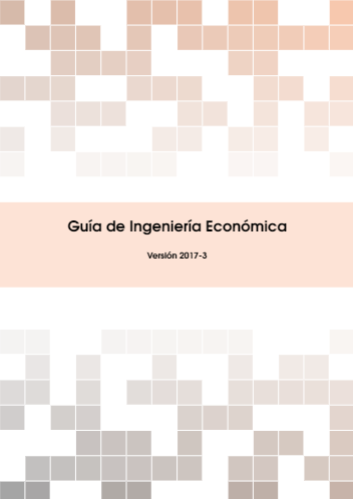
\includegraphics[height=9cm]{img/chAnexos/gingeco.PNG}

\vspace{4mm}
\\ \hline \\
\vspace{2mm}

\noindent Esta guía fue realizada basada en el libro 'Ingeniería Económica' Octava Edición de Guillermo Baca Currea con el propósito de promover el aprendizaje de los temas pertinentes tratados en este texto en cualquier individuo que desee formarse en ellos.\\ \hline \\
\vspace{2mm} La protección del derecho de autor abarcará las expresiones pero no las ideas, procedimientos, métodos de operación o conceptos matemáticos en sí.\\% License information

\noindent \textit{Edición 2017-3}


\clearpage

\chapterimage{ima1} % Table of contents heading image

%\chapterimage{chapter_head_1.pdf} % Table of contents heading image

\pagestyle{empty} % No headers

 \tableofcontents % Print the table of contents itself

\cleardoublepage % Forces the first chapter to start on an odd page so it's on the right

\pagestyle{fancy} % Print headers again


\graphicspath{ {img/} }%imagenes de los capitulos, encabezado y background 

 %-----------------------------------------------------------
 %              TABLA DE NOMENCLATURA
 %------------------------------------------------------
\graphicspath{ {img/tablas}, {img/} }
\begin{center}
\section*{i. Tabla de nomenclatura }
\addcontentsline{toc}{section}{i. Tabla de nomenclaturas }
\end{center}

\begin{spacing}{1}
\begin{center}
\begin{tabular}{ |p{2.5cm}|p{9.5cm}|}
\hline 
\rowcolor{orange!50}
\begin{center} \textbf{Siglas} \end{center} & \begin{center}

\textbf{Nombre}\end{center} \\ \hline     

EA & Efectivo Anual (tasa de referencia SuperFinanciera-nominal anual año vencido- naav)  \\ \hline

g & Gradiente geométrico   \\ \hline

H & Valor incremento escalón monetario  \\ \hline

I & Monto de interés  \\ \hline

IPC & Índice de precios al consumidor \\ \hline

L &  Gradiente aritmético monetario \\ \hline

$i$ & Tasa de interés periódico  \\ \hline

$j$ & Tasa de interés nominal anual (período) vencido  \\  \hline 

i$_{d}$ & Tasa periódica de devaluación \\ \hline
i$_{f}$ & Tasa periódica de la inflación \\ \hline
i$_{r}$ & Tasa periódica real \\ \hline

m$_{1}$ & Número de períodos anuales para  i$_{1}$\\ \hline

m$_{2}$ & Número de períodos anuales para  i$_{2}$\\ \hline

n  & Número de periodos asociados a una i\\ \hline

na(120d)v & Nominal anual (120 días) vencido  \\ \hline

naaa & Nominal anual (año) anticipado\\ \hline  

naav & Nominal anual (año) vencido \\ \hline 

nasa & Nominal anual (semestre) anticipado\\\hline 

nasv & Nominal anual (semestre) vencido\\\hline  

nata & Nominal anual (trimestre) anticipado \\ \hline 

natv & Nominal anual (trimestre) vencido \\ \hline    

na(5a)a & Nominal anual (5 años) anticipado \\ \hline

na(5a)v & Nominal anual (5 años) vencido \\ \hline

na(120d)a & Nominal anual (120 días) anticipado  \\ \hline 

p(120d)v & Periódico (120 días) vencido\\ \hline

paa & Periódico (año)  anticipado \\ \hline

pav & Periódico (año) vencido  \\ \hline 

psa & Periódico (semestre) anticipado \\\hline 

psv & Periódico (semestre) vencido \\\hline

pta & Periódico (trimestre) anticipado \\ \hline 

ptv & Periódico (trimestre) vencido \\ \hline      

p(5a)a & Periódico (5 años) anticipado \\ \hline 

p(5a)v & Periódico (5 años) vencido \\ \hline 

p(120d)a & Periódico (120 días) anticipado  \\ \hline  

R & Cuotas seriales fijas  \\ \hline

SPREAD & Tasa de interés que se adiciona a una tasa de referencia \\ \hline




 
\end{tabular}
\end{center}
\end{spacing}
\ \ \
%\begin{center}
%\section*{Aceptaciones Bancarias}
%\addcontentsline{toc}{section}{Tabla resumen de fórmulas }
%\end{center}
\\ \\ \\ \\ \\ \\ \\
\begin{center} \textbf {Aceptaciones Bancarias (capítulo 3)}\\ \end{center} 

\begin{spacing}{1}
\begin{center}
\begin{tabular}{ |p{2.5cm}|p{9.5cm}|}
\hline 
\rowcolor{orange!50}
\begin{center}\textbf{Siglas} \end{center} & \begin{center} \textbf{Nombre} \end{center} \\ \hline     
 

COM$_{v}$ & Comisión de Venta del Corredor\\ \hline 
i$_{c}$ & Tasa de compra\\ \hline 
i$_{R}$ & Tasa de registro en Bolsa de Valores\\ \hline
i$_{v}$ & Tasa de venta\\ \hline  
P$_{c}$ & Precio del comprador\\ \hline  
P$_{R}$ & Precio de registro\\ \hline  
P$_{v}$ & Precio de venta\\ \hline  
$*$ & Para las ecuaciones de valor el * es un operador que multiplica o desplaza un flujo y/o el resultado del flujo de series uniformes y/o gradiantes diferidos y/o con tiempo muerto (único caso de uso de este operador en esta guía.\\ \hline
 

 
\end{tabular}
\end{center}
\end{spacing}

\\ \\ \\

\begin{center} \textbf {Operadores lógicos}\\ \end{center} 

\begin{spacing}{1}
\begin{center}
\begin{tabular}{ |p{2.5cm}|p{9.5cm}|}
\hline 
\rowcolor{orange!50}
\begin{center}\textbf{Siglas} \end{center} & \begin{center} \textbf{Nombre} \end{center} \\ \hline 

$ Q \Leftarrow P $ & "Q dado que P", "Q si P", "Q siempre que P" \\ \hline

$ P \Rightarrow Q $ & "P implica Q", "Si P, entonces Q", "P sólo si Q" \\ \hline

$ P \Leftrightarrow Q $ & "P si y sólo si Q", "P es necesario y suficiente para Q", 
     "P es equivalente con Q"\\ \hline

$ \therefore P $ &  "Porque P" \\ \hline

$ \therefore  P $ & "Por lo tanto, P" \\ \hline

$\equiv$ & Equivalente \\ \hline

\end{tabular}
\end{center}
\end{spacing}
\newpage
 %-----------------------------------------------------------
 %              TABLA DE FORMULAS
 %------------------------------------------------------

\begin{center}
\section*{ii. Tabla resumen de fórmulas}
\addcontentsline{toc}{section}{ii. Tabla resumen de fórmulas trabajadas en la guía}
\end{center}

\begin{spacing}{1}
\begin{center}
\begin{tabular}{ |p{7cm}|p{7cm}|}
\hline 
\rowcolor{orange!50}

\begin{center}\textbf{Fórmula} \end{center} & \begin{center} \textbf{Nombre} \end{center}  \\ \hline

$(1 + i_{1})^{m_1} = (1 + i_{2})^{m_2}$ & Equivalencia de tasas periódicas\\\hline 

$i_{r} = i_{1} + i_{2} + i_{1}i_{2}$ & Tasa de interés periódica real\\ \hline
$i_r = \frac{i - i_f}{1 + i_f}$ & Tasa de interés real\\ \hline 

$j = im$  &  Tasa interés nominal anual vencida\\ \hline   
 

$i_a = \frac{i}{1 + i}$  & Tasa de interés periódica anticipada\\ \hline   

 $i = \frac{i_a}{1 - i_a}$ & Tasa de interés periódica vencida\\ \hline   
$D = Fdn$ & Valor de descuento dado un flujo (F)\\ \hline
  
 $F = P(1 + i)^n$ & Valor futuro\\ \hline 

 $VP = R  \frac{1-(1 + i)^{-n}}{i} $ & Valor presente serie uniforme vencida\\ \hline 

$VP_{a} = R  \frac{1-(1 + i)^{-n}}{i}  (1 + i) $ & Valor presente serie uniforme anticipada\\ \hline 

$VF = R  \frac{(1 + i)^n-1}{i} $ & Valor futuro serie uniforme vencida\\ \hline   
$VF_{a} = R  \frac{(1 + i)^n-1}{i}(1 + i) $ & Valor futuro serie uniforme anticipada\\ \hline 

$VP = \frac{R}{i}$ & Valor presente serie perpetua vencida\\ \hline 
$VP = R  \frac{1-(1 + i)^{-n}}{i} + \frac{L}{i}[ \frac{1-(1 + i)^{-n}}{i} - n(1 + i)^{-n} ]$ & Valor presente de gradiente aritmético\\ \hline 
 $VF = R  \frac{(1 + i)^{n} - 1}{i} + \frac{L}{i}[ \frac{(1 + i)^n - 1}{i} - n ]$ &  Valor futuro de gradiente aritmético\\ \hline 
$VP = \frac{R}{i} + \frac{L}{i^2}$ & Valor presente gradiente aritmético infinito\\ \hline 
$VP = R  \frac{(1 + g)^n  (1 + i)^{-n}-1}{g - i} $ & Valor presente de gradiente geométrico, si $g \neq i$\\ \hline 
$VP = \frac{Rn}{1 + i}$ & Valor presente gradiente geométrico si $g = i$\\ \hline 
$VF = R  \frac{(1 + g)^n - (1 + i)^n}{g - i} $ & Valor futuro gradiente geométrico si $g \neq i$\\ \hline 
$VF = Rn(1 + i)^{n-1} $ & Valor futuro gradiente geométrico si $g = i$\\ \hline 
$VP = \frac{R}{1 - g} $ & Valor presente gradiente geométrico infinito si $g < i$\\ \hline
 $VP = \infty $ & Valor presente gradiente geométrico infinito si $g \geq i$ &\\ \hline 
 
\end{tabular}

\clearpage
		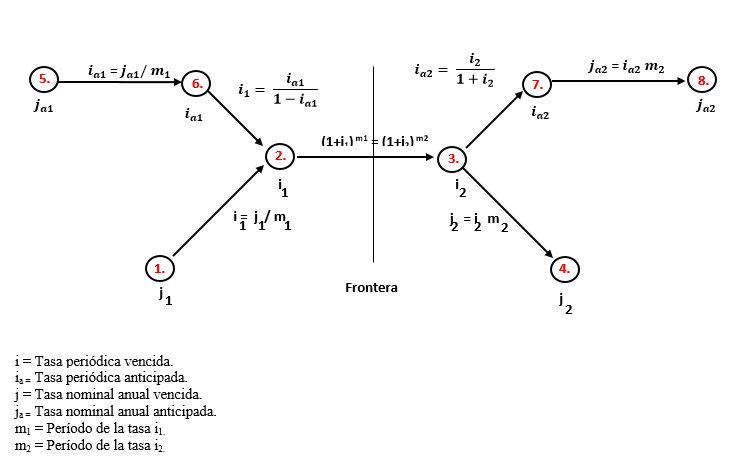
\includegraphics[width = 10.0 cm]{general}\\
		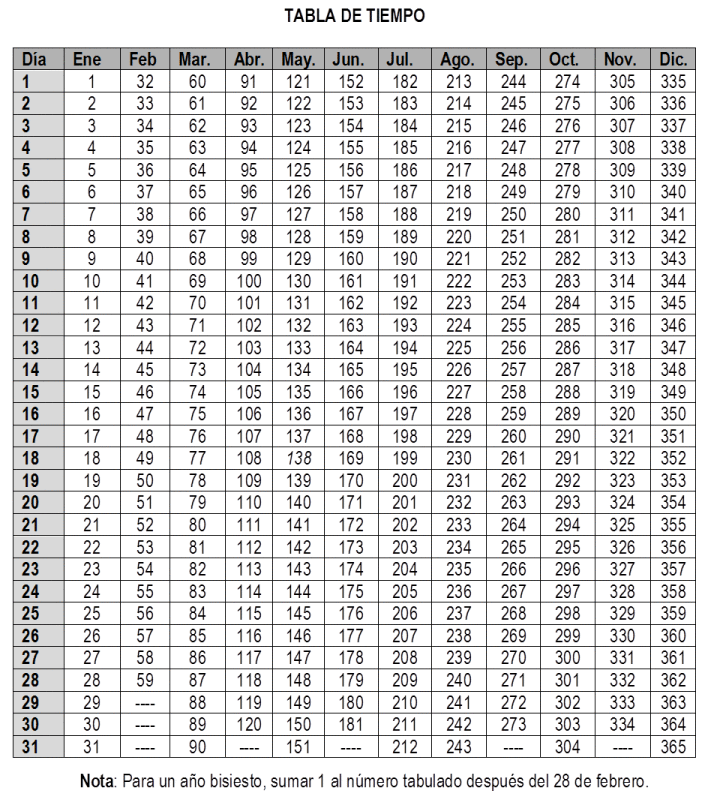
\includegraphics[height=15cm]{TTime}
\end{center}
\end{spacing}

\clearpage

\begin{center}
\section*{iii. Tabla resumen de fórmulas}
\addcontentsline{toc}{section}{iii. Tabla funciones de Excel}
\end{center}

\vspace{2cm}

\begin{spacing}{1}
\begin{center}
\begin{tabular}{ |p{7cm}|p{5.5cm}|}
\hline 
\rowcolor{orange!50}

\begin{center}\textbf{Nombre} \end{center}  & \begin{center} \textbf{Función Financiera en Excel} \end{center}  \\ \hline

Equivalencia de tasas periódicas &  TASA(m;;-1;1+i)\\\hline 

Tasa interés nominal anual vencida & TASA.NOMINAL(i;m) \\ \hline

Tasa interés periódica año vencido & INT.EFECTIVO(j;m) \\ \hline

Valor futuro & VF(i;n;;VA,0)\\ \hline 

Valor presente & VA(i;n;;VF,0)\\ \hline 

Valor presente serie uniforme vencida & VNA(i;R1;R2;R3;...) \\ \hline  

Valor futuro serie uniforme vencida &  VF(i;n;;VA,0)\\ \hline

Valor futuro serie uniforme anticipada & VF(i;n;;VA,1)\\ \hline 

Valor presente serie perpetua vencida & VA(i;n;R;0) \\ \hline

Valor presente gradiente aritmético & VNA(i;R1;R2;R3;...) \\ \hline

Valor presente gradiente geométrico & VNA(i;R1;R2;R3;...) \\ \hline

Valor cuota serie uniforme vencida & PAGO(i;n;P;F;0) \\ \hline

Valor cuota serie uniforme anticipada & PAGO(i;n;P;F;1) \\ \hline

Ecuación de valor & Función Buscar Objetivo\\ \hline


\end{tabular}
\end{center}
\end{spacing}

\clearpage
\graphicspath{ {img/ch0/}, {img/} }

\section*{\textcolor{Blue}{iii. Guía para resolver ejercicios de Ingeniería Económica a partir de la evaluación conceptual}}
\addcontentsline{toc}{section}{iii. Guía para resolver ejercicios de Ingeniería Económica}
\begin{enumerate}
    \item Leer y precisar el enunciado del ejercicio, resaltando las variables independientes, dependientes y los elementos constitutivos para el flujo de caja o diagrama de equivalencia.
    \item Volver a leer para determinar los bloques conceptuales(ejemplo: serie  uniforme proyectada y diferida)
    \item A partir de los bloques determinar primero los subindices de n, luego determinar subindices de valores o series que corresponden a las n.
    \item Estructurar la solución en forma ordenada en 5 pasos: Diagrama de flujo de caja o de equivalencia, declaración de variables, declaración de fórmulas, desarrollo matemático (ECUACIÓN DE VALOR o de equivalencia), respuesta (justificación).
    \textcolor{Blue}{\item \textbf{Construir el diagrama de flujo de caja, mediante:}}
    \begin{itemize}
        \color{Blue}
        \item Un plano cartesiano, para n períodos vencidos o anticipados según el caso y para el actor de referencia (prestamista o prestatario).
        \item El dibujo de los egresos en sentido negativo del eje y, y los ingresos en sentido positivo del eje y.
        \item A la existencia de egresos habrá un ingreso o varios ingresos para poder existir una ecuación de valor.
        \item Una línea horizontal u oblicua que una el flujo final al flujo inicial de la serie uniforme o serie escalonada o gradiente.
        \item Una fecha focal (ff) al final o al comienzo o al intermedio del eje x, que permita visualizar y registrar la ECUACIÓN DE VALOR en el desarrollo matemático.
        \item Los bucles que direccione el sentido positivo (valor futuro) o negativo (valor presente) del valor de equivalencia con respecto a la fecha focal.
        \item Los bucles, en su interior, indicar el n (número de períodos positivos - valor futuro-, negativos - valor presente) a \underline{trasladar a la derecha o izquierda} el componente de la ecuación de valor. Ante la existencia de ``períodos muertos'' en series, gradientes, cambios de tasas u otros, no olvidar ``trasladar'' el VP o VF de la serie, gradiente, etc, a la ff mediante el operador fundamental $P=F(1+i)^{-n}$, según el caso.
        \item La tasa periódica porcentual (i\%) o la tasa periódica anualizada (j\%) de los bucles vencida o anticipada según la modalidad de los períodos. IMPORTANTE: la periodicidad y modalidad de la tasa de interés (i\%) debe ser igual a las de los períodos (n). En su defecto, utilizar la fórmula de conversión de tasas (i\%) y/o de cambio de modalidad (ia\% a i\%).
    \end{itemize}
    \item Declarar las variables, mediante el registro de:
    \begin{itemize}
        \item Las variables independientes, indicando las unidades de cada una, la periodicidad y modalidad de liquidación de intereses y períodos.
        \item La variable o variables dependientes, indicando las unidades y el signo de interrogación.
        \item La verificación de las variables necesarias para la aplicación de las fórmulas.
    \end{itemize}
    \item Declarar las fórmulas, indicando:
    \begin{itemize}
        \item Las fórmulas transitorias y las fundamentales a utilizar, acompañadas del NOMBRE de la misma. 
    \end{itemize}
    \textcolor{Blue}{\item \textbf{Desarrollar el procedimiento matemático, efectuando:}}
    \begin{itemize}
        \color{Blue}
        \item El remplazo matemático de las fórmulas e indicando las unidades correspondientes. 
        \item El registro de la expresión de ECUACIÓN DE VALOR o equivalencia al remplazo matemático correspondiente.
        \item El proceso matemático en forma ordenada, clara y precisa. \\
    \end{itemize}
    \item Registrar la respuesta (justificación), indicando:
    \begin{itemize}
        \item La variable independiente o variables independientes, su respuesta y unidades. \\
    \end{itemize}
\end{enumerate}

\textcolor{Blue}{\textbf{IMPORTANTE 1:}} Volver a leer el enunciado del ejercicio para reconfirmar la respuesta y la justificación. \textbf{\textcolor{ForestGreen}{VALIDAR}} el ejercicio utilizando las fórmulas \textcolor{ForestGreen}{ALGEBRÁICAS} de \textcolor{ForestGreen}{EXCEL}, \textbf{\textcolor{ForestGreen}{FÓRMULAS FINANCIERAS}} de \textcolor{ForestGreen}{EXCEL} y \textbf{\textcolor{ForestGreen}{CRYSTAL BALL}}.\\

\textcolor{Blue}{\textbf{IMPORTANTE 2:}} Aplicar los conceptos de la guía INGECO para articular los formatos y herramientas financieras que requiere fondo emprender en sus convocatorias para financiar planes de negocios como modalidad de grado emprendimiento (Acuerdo 38 de 2015 consejo Académico U Distrital)

\section*{\textcolor{ForestGreen}{iv. Guía para resolver ejercicios de Ingeniería Económica a partir de Excel financiero}}
\addcontentsline{toc}{section}{iv. Guía para resolver ejercicios a partir de Excel financiero}

\begin{enumerate}
    \item Leer y precisar el enunciado del ejercicio, resaltando las variables independientes, dependientes y los elementos constitutivos para el flujo de caja o diagrama de equivalencia. 
    \item Volver a leer para determinar los bloques conceptuales (ejemplo: serie uniforme proyectada y diferida).
    \item A partir de los bloques determinar primero los subíndices de n, luego determinar subíndices de valores o series que corresponden a las n.
    \item Estructurar la solución en forma ordenada en 5 pasos: Declaración de variables, tabla de flujo de caja o tabla de amortización o capitalización de ser necesario, aplicación de fórmulas financieras en Excel, respuesta (justificación) y gráfica.
    \textcolor{ForestGreen}{\item \textbf{Declarar variables mediante el registro de:}}
    \begin{itemize}
        \color{ForestGreen}
        \item Las variables independientes, indicando las unidades de cada una, la periodicidad y modalidad de liquidación de intereses y períodos.
        \item La variable o variables dependientes, indicando las unidades y dejando la celda de estas con un 0.
        \item La verificación de las variables necesarias para la aplicación de la formula.
    \end{itemize}
    \textcolor{ForestGreen}{\item \textbf{Realizar la tabla de flujo de caja de la siguiente forma:}}
    \begin{itemize}
        \color{ForestGreen}
        \item Definir en la columna [1] el número de períodos correspondientes al ejercicio.
        \item En la columna [2] rellenar con el flujo correspondiente a cada período en la columna [1]. 
    \end{itemize}
    \begin{center}
    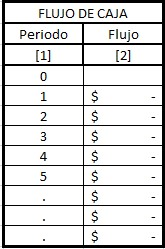
\includegraphics[height=6cm]{0_1}
    \end{center}
    
    En el caso de ser una tabla de amortización se debe rellenar de la siguiente forma: 
    \begin{itemize}
        \color{ForestGreen}
        \item Para todos los valores de [3], [4], [5], [6] en el período 0 se les asignara un valor de \$0.
        \item Definir en la columna [1] el número de períodos correspondientes al ejercicio.
        \item Definir en la columna [2] para el período 1 el valor es igual al rezagado de [6] y arrastrar para todos los períodos.
        \item Definir en la columna [3] para el período 1 el valor de [1] multiplicado por la celda fija en la que se encuentran los intereses y arrastrar para todos los períodos.
        \item Definir en la columna [4] para el período 1 el valor de [5] menos el valor de [6] y arrastrar para todos los períodos.
        \item Definir en la columna [5] el valor de la cuota correspondiente para cada [1] y arrastrar para todos los períodos.
        \item Definir en la columna [6] el valor de [1] menos el valor de [4] y arrastrar para todos los períodos.
    \end{itemize}
    \begin{center}
    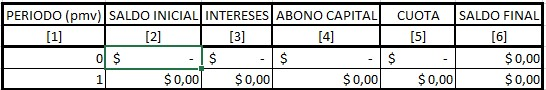
\includegraphics[height=2.35cm]{0_2}
    \end{center}
    
    En el caso de tener una tabla de capitalización de debe rellenar de la siguiente forma:
    \begin{itemize}
        \color{ForestGreen}
        \item Para todos los valores de [1], [2], [3], [4], [5], [6] en el período 0 se les asignara un valor de \$0.
        \item Definir en la columna [1] el número de períodos correspondientes al ejercicio.
        \item Definir en la columna [2] para el período 1 el valor es igual al rezagado de [5] y arrastrar para todos los períodos.
        \item Definir en la columna [3] para el período 1 el valor de la cuota correspondiente para cada [1] y arrastrar para todos los períodos.
        \item Definir en la columna [4] para el período 1 el valor de [2] más el valor [3] multiplicando por la celda fija en la que se encuentran los intereses y arrastrar para todos los períodos.
        \item Definir en la columna [5] para el período 1 la suma de [2], [3] y [4].
    \end{itemize} 
    \begin{center}
    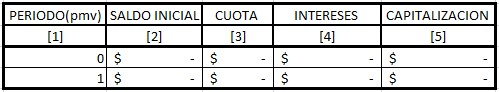
\includegraphics[height=2.5cm]{0_3}
    \end{center}
    \textcolor{ForestGreen}{\textbf{NOTA:} Es una buena idea referenciar todos los valores que se apliquen en el flujo de caja desde la declaración de variables, así al cambiar un valor de la declaración de variables cambiará toda la tabla del flujo de caja y de esta forma se puede aplicar análisis de sensibilidad al ejercicio.} \\ \\ 
    
    \textcolor{ForestGreen}{\item \textbf{Para la aplicación de fórmulas financieras en Excel se deberá tener en cuenta cuál fórmula deberá usarse a partir de las siguientes:}} \\
    

    \begin{enumerate}
    \renewcommand{\labelenumi}{\roman{enumi}}
        \item \textcolor{ForestGreen}{PAGO:} Calcula el pago de un préstamo basado en pagos y tasa de interés constante.
        \begin{center}
        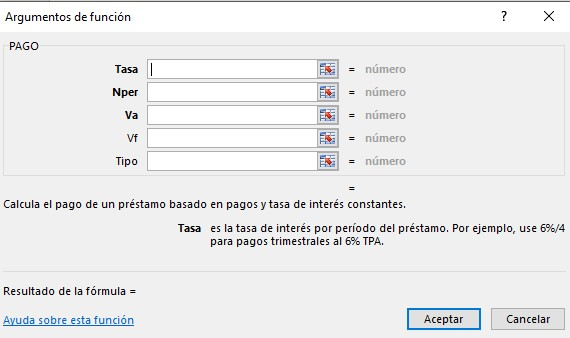
\includegraphics[height=6cm]{0_4} \\
        \end{center}
        \begin{center}
        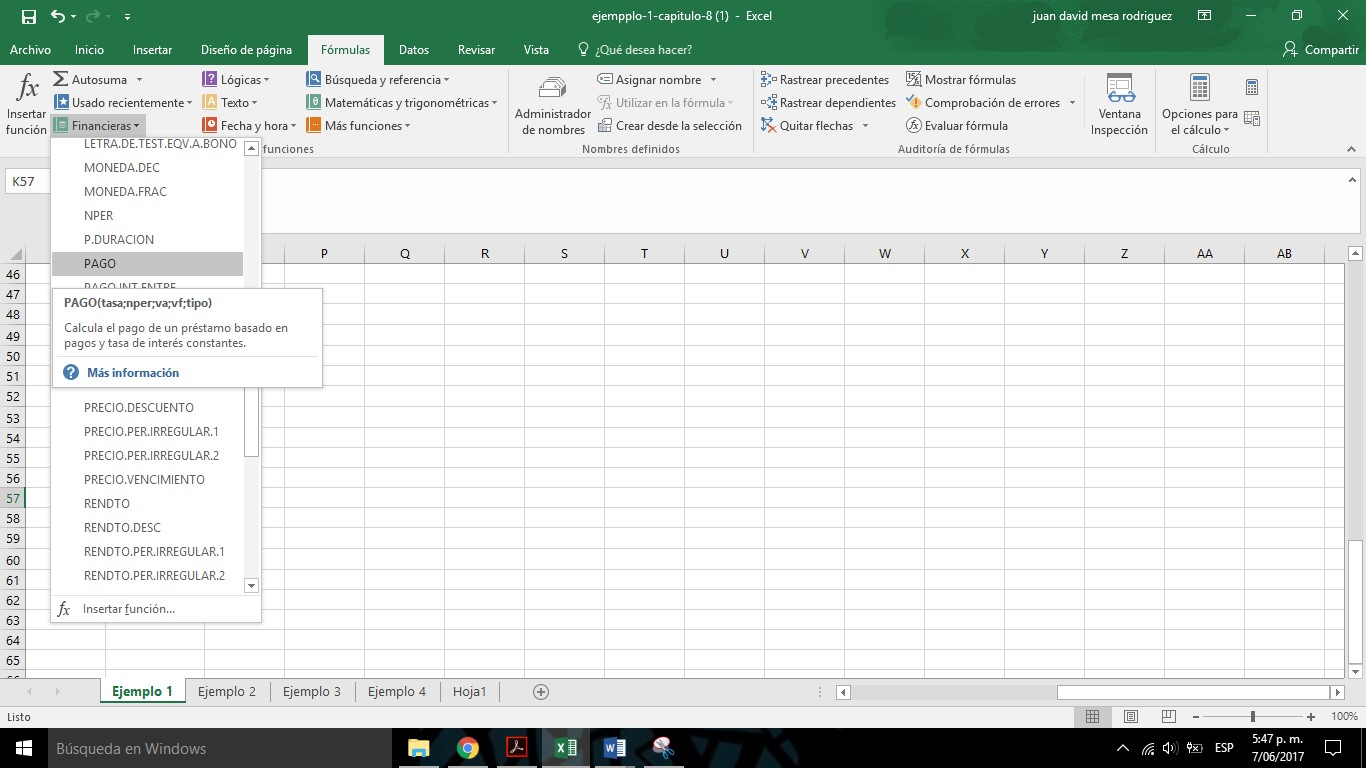
\includegraphics[height=7.41cm]{0_5} 
        \end{center}
        \item \textcolor{ForestGreen}{VA (Valor actual):} Devuelve el valor presente de una inversión; la suma total del valor actual de una serie de pagos futuros.
        \begin{center}
        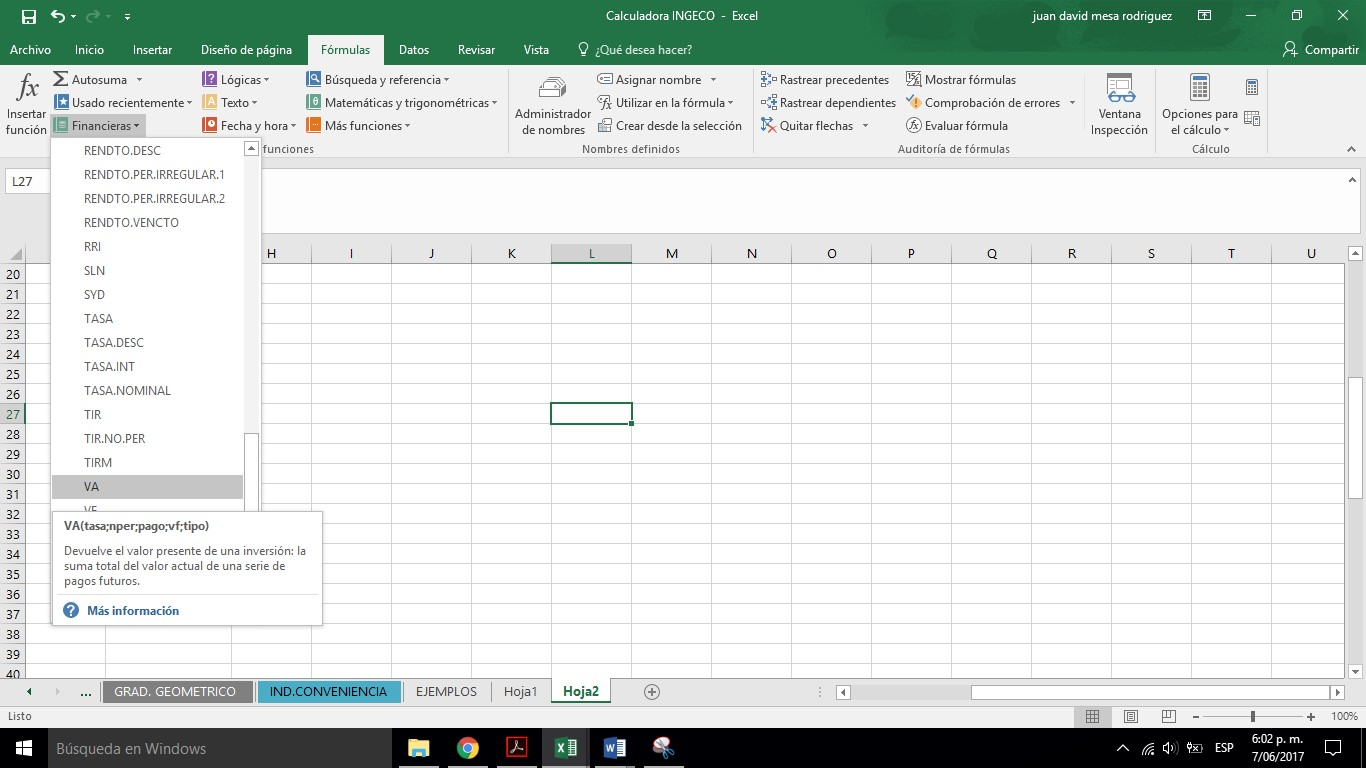
\includegraphics[height=7.41cm]{0_6} \\
        \end{center}
        \begin{center}
        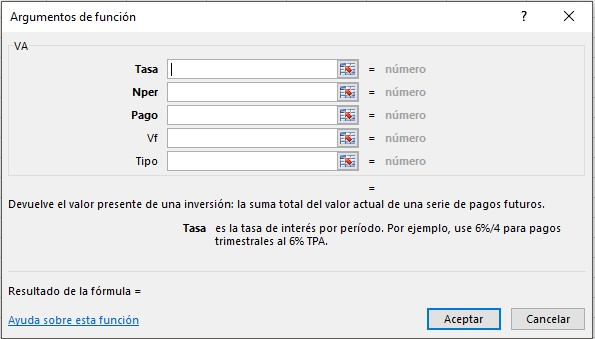
\includegraphics[height=6cm]{0_7}
        \end{center}
        \item \textcolor{ForestGreen}{VF (Valor futuro):} Devuelve el valor futuro de una inversión basado en pagos periódicos y constantes, y una tasa de interés también constante.
        \begin{center}
        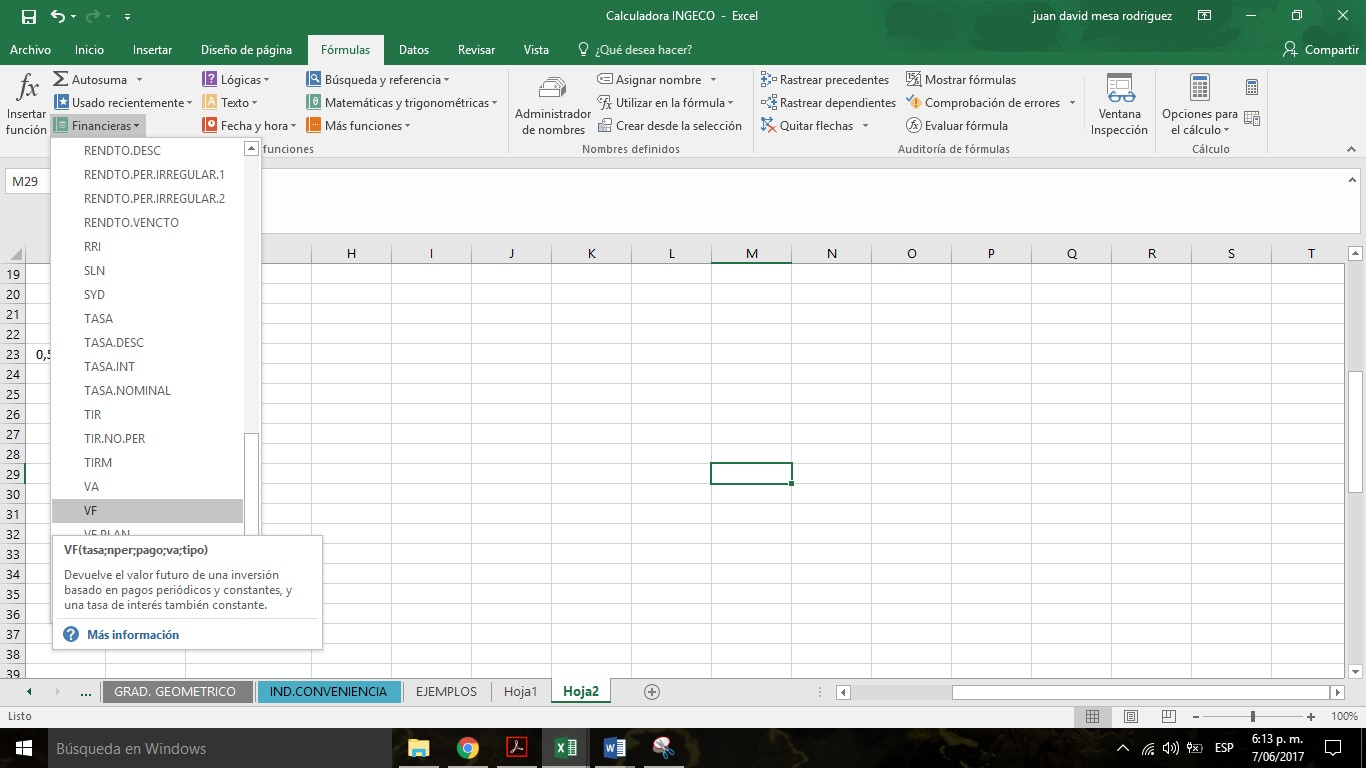
\includegraphics[height=7.15cm]{0_8} \\
        \end{center}
        \begin{center}
        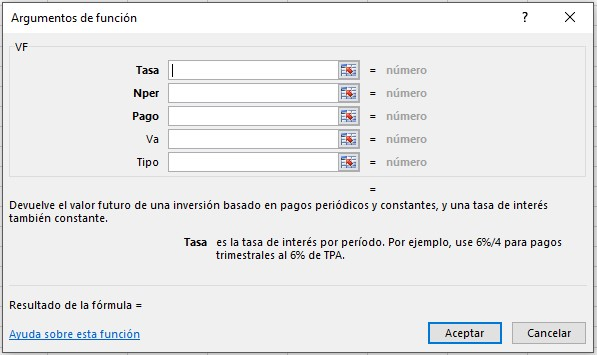
\includegraphics[height=6cm]{0_9}
        \end{center}
        \item \textcolor{ForestGreen}{TASA:} Devuelve el valor de la tasa de interés por período de un préstamo o una inversión.
        \begin{center}
        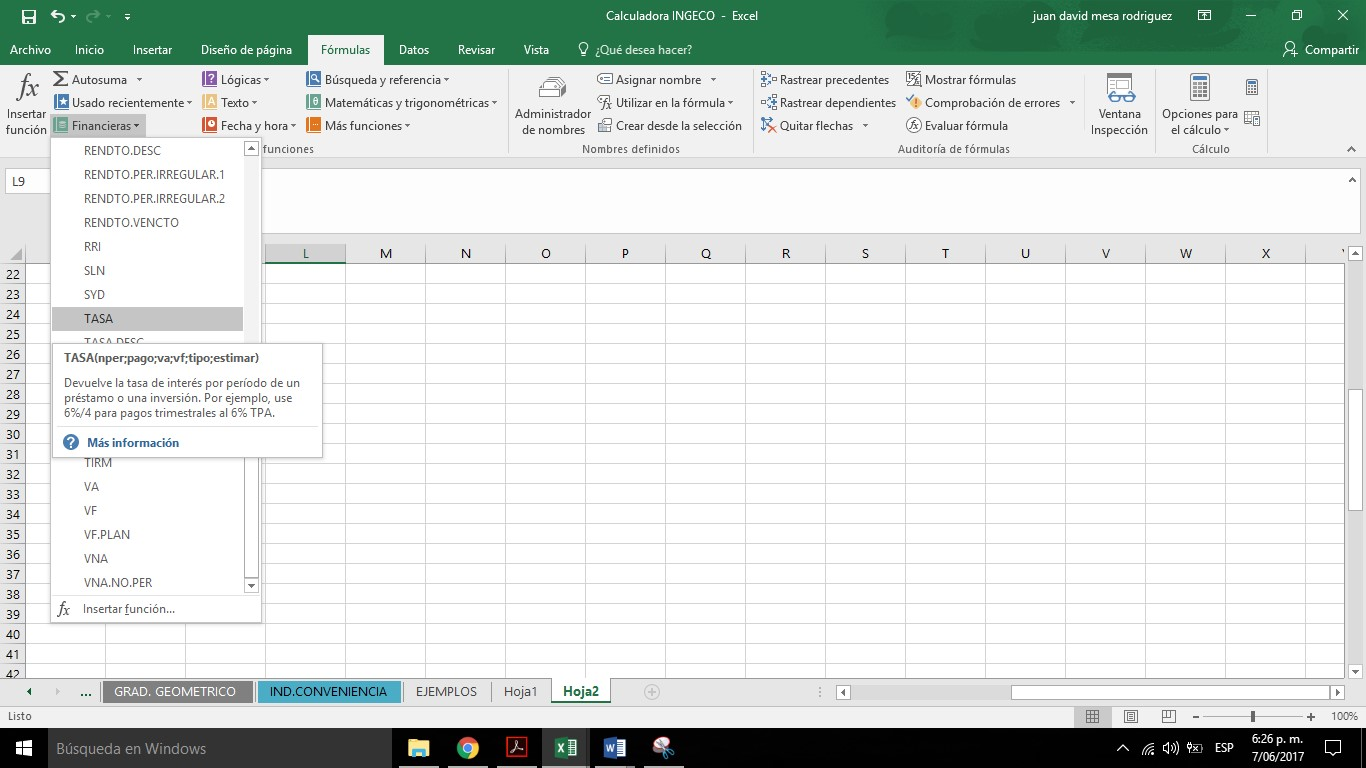
\includegraphics[height=7.15cm]{0_10} \\
        \end{center}
        \begin{center}
        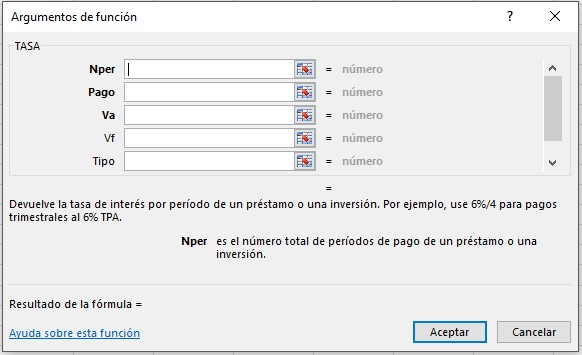
\includegraphics[height=6cm]{0_11}
        \end{center}
        \item \textcolor{ForestGreen}{NPER (Numero de períodos):} Devuelve el número de pagos de una inversión, basado en pagos constantes y periódicos y una tasa de interés constante.
        \begin{center}
        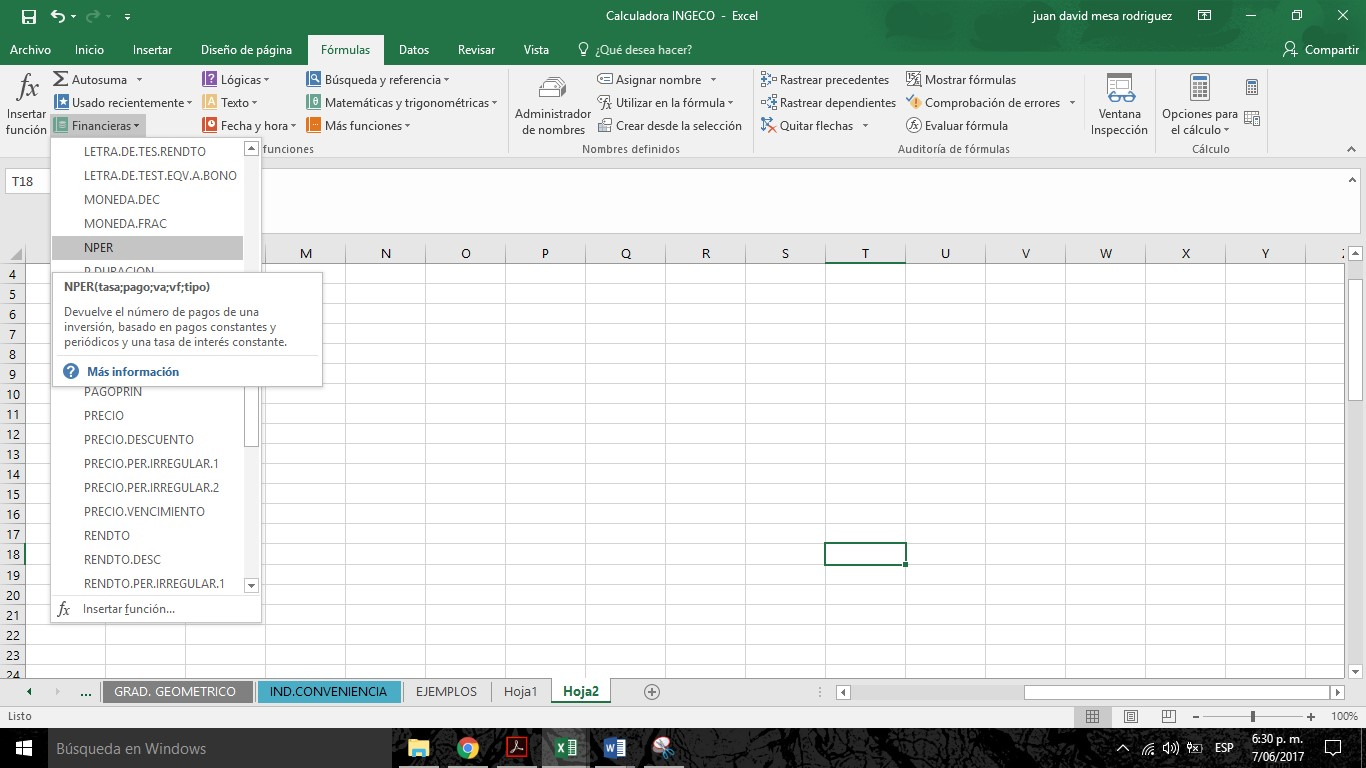
\includegraphics[height=7.15cm]{0_12} \\
        \end{center}
        \begin{center}
        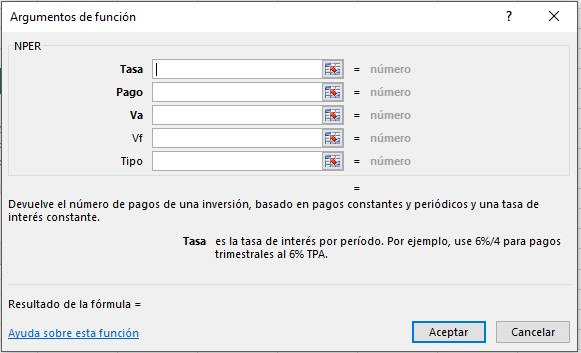
\includegraphics[height=6cm]{0_13}
        \end{center}
        \item \textcolor{ForestGreen}{INT. EFECTIVO (Interés efectivo):} Devuelve la tasa de interés anual efectiva.
        \begin{center}
        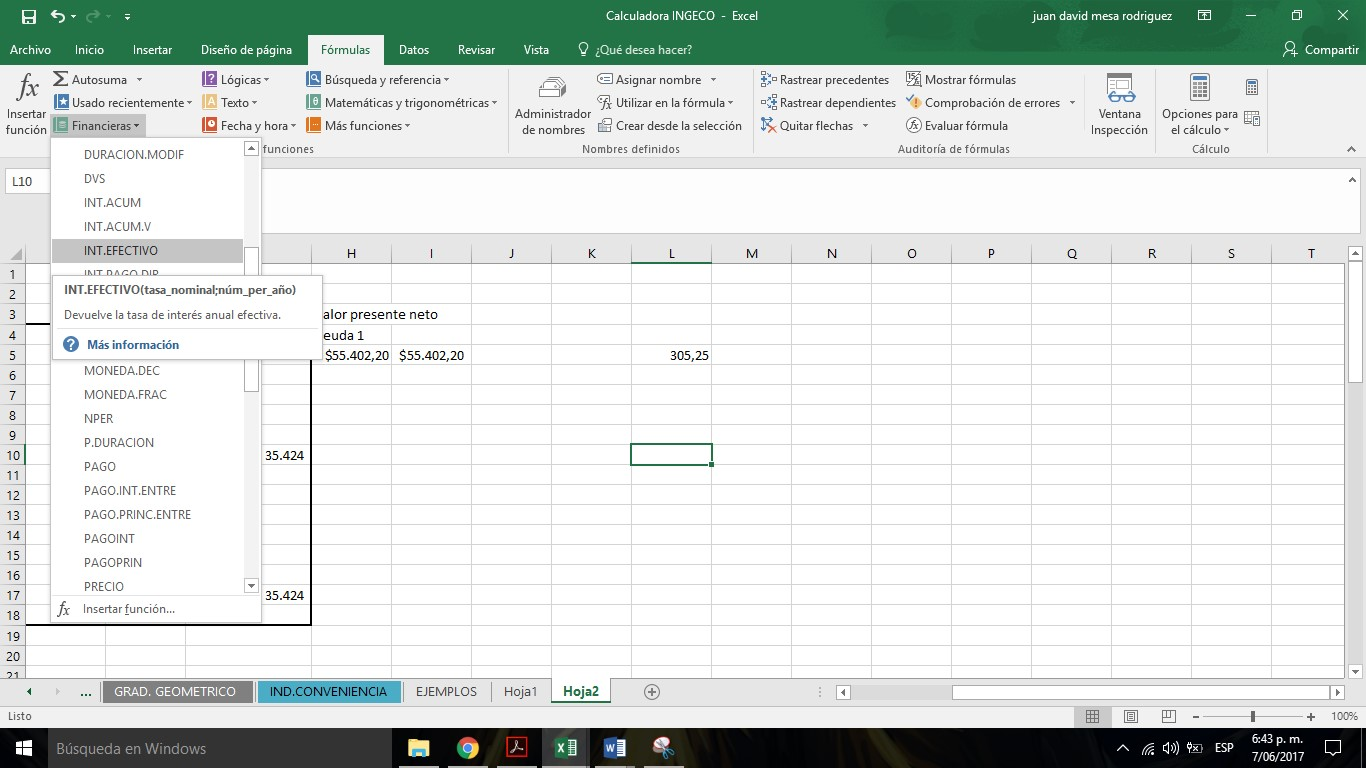
\includegraphics[height=7.15cm]{0_14} \\
        \end{center}
        \begin{center}
        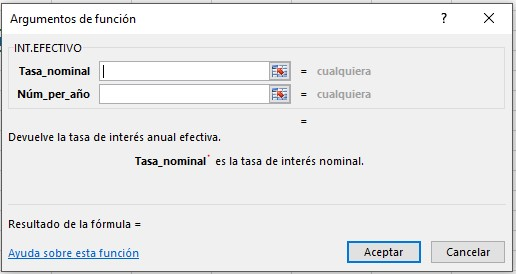
\includegraphics[height=6cm]{0_15}
        \end{center}
        \item \textcolor{ForestGreen}{TASA.NOMINAL:} Devuelve la tasa de interés nominal anual. 
        \begin{center}
        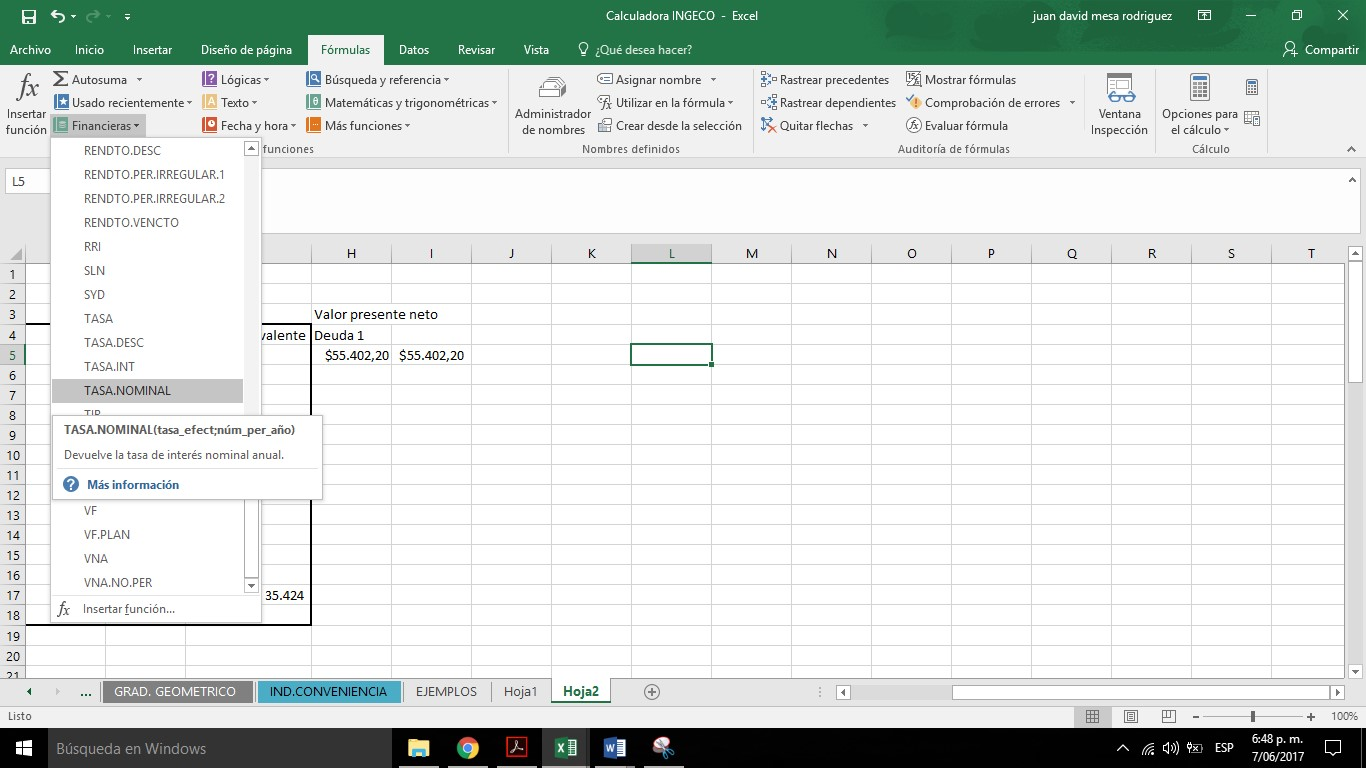
\includegraphics[height=7.15cm]{0_16} \\
        \end{center}
        \begin{center}
        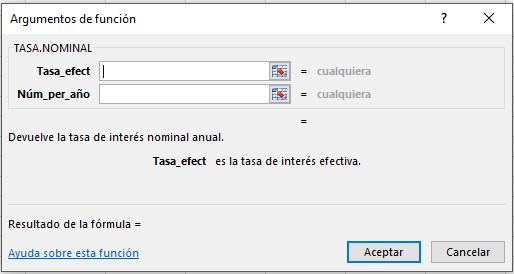
\includegraphics[height=6cm]{0_17}
        \end{center}
        \item \textcolor{ForestGreen}{BUSCAR OBJETIVO:} Encuentra la entrada adecuada para el valor que desee. 
        \begin{center}
        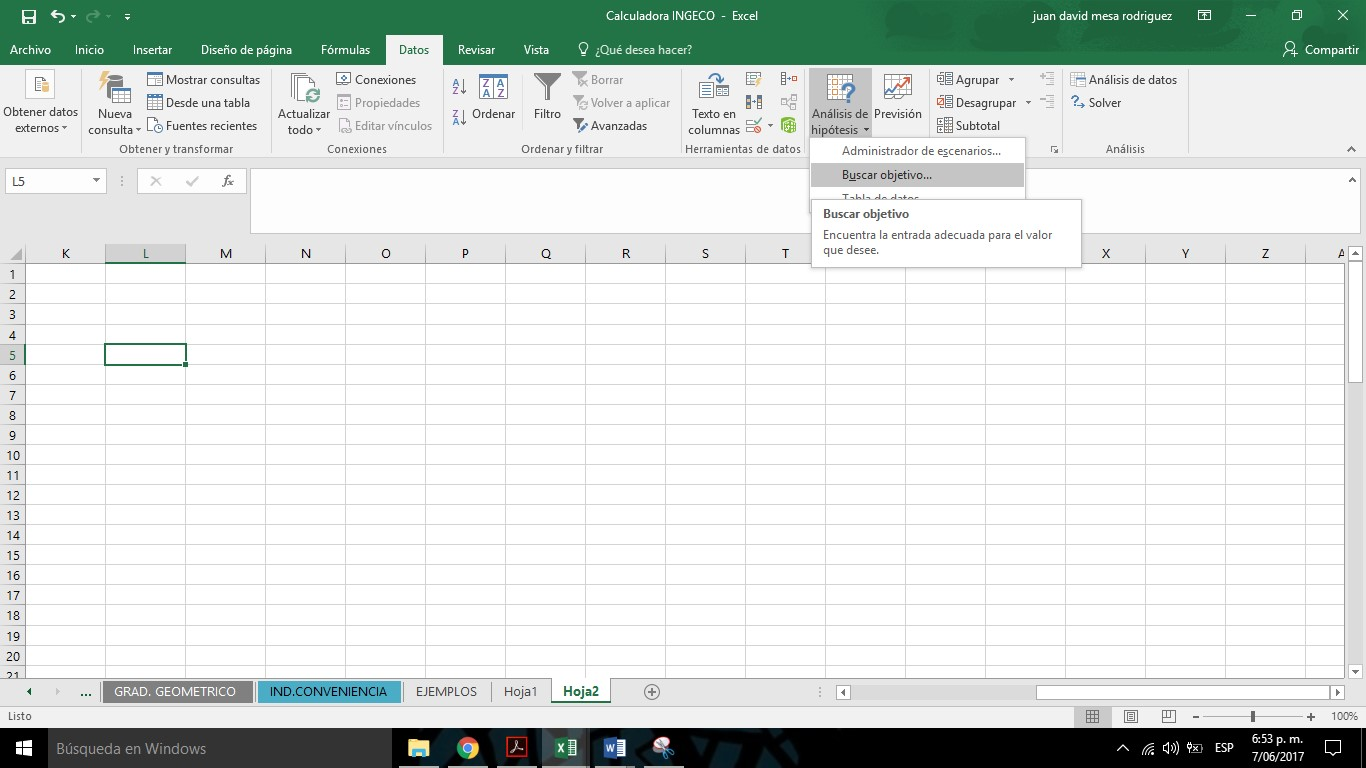
\includegraphics[height=7.15cm]{0_18} \\
        \end{center}
        En la opción de \textcolor{ForestGreen}{“Definir la celda”} se debe colocar la celda sobre la que se encuentra la variable sobre la que se conoce el valor que se desea obtener. \\
        En la opción de \textcolor{ForestGreen}{“Con el valor”} se debe colocar el valor que se desea obtener sobre la variable presente en la opción “Definir la celda”. \\
        En la opción de \textcolor{ForestGreen}{“Cambiando la celda”} se debe colocar la celda que posee la variable que se desea cambiar para llegar al valor que se encuentra en la opción \textcolor{ForestGreen}{“Con el valor”}. \\
        Una vez definidas las opciones Excel realizará los cálculos necesarios y devolverá los valores encontrados sobre las celdas colocadas en la fórmula. \\ \\ 
    
        \begin{center}
        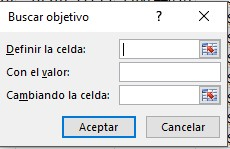
\includegraphics[height=5cm]{0_19}
        \end{center}
    \end{enumerate}
    
    \textcolor{ForestGreen}{\item \textbf{Registrar la respuesta (justificación) indicando:}}
    \begin{itemize}
        \color{ForestGreen}
        \item La variable independiente o variables independientes, su respuesta y unidades.
    \end{itemize}

    \textcolor{ForestGreen}{\item \textbf{Realizar la gráfica correspondiente de la siguiente forma:}}
    \begin{itemize}
        \color{ForestGreen}
        \item La gráfica debe mostrar el comportamiento de los ingresos o egresos a través del número de períodos que posea el problema (Dinero vs Períodos).
        \item Este debe poseer el título del gráfico, los títulos de los ejes y líneas de cuadrícula. 
        \item Se debe especificar las unidades que posee cada eje.
    \end{itemize}


\end{enumerate}



\part{Capítulo uno}
%\graphicspath{ {img/} }

%----------------------------------------------------------------------------------------
%	CHAPTER 1
%----------------------------------------------------------------------------------------

\chapterimage{ima2} % Chapter heading image



\chapter{Interés simple}


\section{Fórmulas de capítulo }

\begin{spacing}{1.5}
\begin{center}
\begin{tabular}{ |p{6cm}|p{5cm}| p{4cm}|}
\hline 
\rowcolor{orange!50}
\begin{center}\textbf{Fórmula} \end{center} & \begin{center} \textbf{Nombre}\end{center} & \begin{center} \textbf{Excel} \end{center} \\ \hline                        

I = Pin & Valor interés simple & TASA.INT(ni;nf;P)\\ \hline

F = P+I & Valor futuro &  - \\ \hline 

P= $\frac{F}{1+ni }$ & Valor presente & - \\ \hline

F= P(1+in) & Valor futuro  & - \\ \hline

P= F(1-dn) & Valor presente de un flujo futuro & - \\ \hline

F= P/(1-dn) & Valor futuro de un flujo presente & - \\ \hline

VL= F(1-dn) & Valor líquido dado un flujo futuro & - \\ \hline

 
\end{tabular}
\end{center}
\end{spacing}

\section{Introducción}
En este capítulo daremos definiciones y conceptos básicos utilizados en las finanzas, los cuales serán indispensables para el desarrollo de la guía. Este enfoque analítico nos permite la optimización de los recursos económicos, lo cual viene a ser el objetivo final de esta guía.

\section{Valor del dinero a través del tiempo}
No es lo mismo tener hoy \$100.000 que tener \$100.000 dentro de un año, porque lo que hoy se puede hacer con ese dinero es más de lo que se podrá hacer dentro de un año debido a que normalmente todos los artículos suben de precio, por tal motivo cuando se habla de una suma de dinero debe especificarse la fecha o de lo contrario la información es incompleta. Lo anterior se puede expresar en una forma muy simple: El dinero cambia de valor a través del tiempo.
\\\\
El concepto anterior está íntimamente ligado con el concepto de equivalencia que consiste en que, sumas de dinero diferentes en épocas distintas tienen el mismo poder adquisitivo, así por ejemplo si dentro de un año necesito \$120.000 para hacer lo que hoy hago con \$100.000 entonces diré que estas sumas son equivalentes en el tiempo.

\section{Interés (I)}

Todos los bienes son susceptibles de ser entregados a otra persona en arriendo y por ello cobrar un canon de arrendamiento, por lo que es posible dar una casa en arriendo y cobrar una suma mensual por el uso de esa casa, también es posible entregar en arriendo un vehículo o una máquina etc. De la misma forma es posible entregar en arriendo un dinero y el canon del arrendamiento del dinero recibe el nombre de interés el cual representaremos por I.
\\\\
Otra forma de ver el concepto de interés es como la retribución económica que devuelve el capital inicial por período transcurrido, de forma tal que compense la desvalorización de la moneda, que cubra el riesgo y que pague el alquiler del dinero como premio al dueño por no haberlo consumido.

\section{Tasa de interés periódico (i)}
Es el porcentaje (\%) que se paga por el alquiler del dinero, lo representaremos por i . Por ejemplo si tengo que pagar \$4 de interés por un préstamo de \$100 en un año, entonces la tasa de interés será del 4 \% período anual vencido que se puede escribir como 4\% pav y si tengo que pagar 3 centavos por el préstamo de \$1 la tasa será  3\% pav o equivalente a 0,03 pav.

\section{Tiempo (t)}
Es la duración de la inversión; y lo representaremos por $t$ y no por $n$ que corresponde al período de ingreso o pago de interés. % el período de liquidación de los intereses. En interés simple la unidad de tiempo es el año.

\section{Período (n)}
Tiempo unitario de liquidación de intereses, puede ser diario, semanal, mensual, bimensual, trimestral, semestral, anual, bianual, entre otros. %El periodo es equivalente = Días de liquidación de Intereses/ Días del año 

\section{Capital inicial (P)}
Es la cantidad de dinero que se invierte, también se le conoce con el nombre de principal, valor actual, valor inicial o valor presente y lo representaremos por P.

\section{Postulado básico de las finanzas}
El postulado básico de las finanzas establece que el interés es una función directa que depende de 3 variables: el capital inicial (\textit{mientras más grande sea el capital mayor deberá ser el interés) la tasa (la tasa depende de las fuerzas del mercado, cuando hay escasez de dinero o cuando los precios en general están al alza la tasa será mayor) y del tiempo (mientras más tiempo dure la inversión mayor será el interés}). Ver la tasa EA de la SuperFinanciera.

\section{Fórmula de interés (I)}
De acuerdo con el postulado anterior podemos establecer la siguiente ecuación:
\begin{equation}
I = Pin \hspace{35pt} \textit{Valor interés simple (I)}
\end{equation}

\section{Gráfica de flujo de caja}
\textit{A fin de facilitar la comprensión de los problemas mediante una gráfica, se ha adoptado la siguiente convención: la línea horizontal representa el tiempo y allí escribiremos las fechas y los períodos de tiempo; de esta línea salen unas flechas hacia arriba y otras hacia abajo, las que están hacia arriba representan ingresos y las que están hacia abajo representan egresos}.
\\\\
\textit{Nota.} En este texto las fechas las daremos en la forma:  AAAA-MM-DD (Año-mes-día) por ejemplo, el día 15 de septiembre de 1998 1o representaremos así:         15-09-98

\section{Capital final (F, i, n, P)}
Es el capital inicial más los intereses, también se le denomina monto, valor final, valor futuro, la suma o acumulado y lo representaremos por $F$. De acuerdo a la definición la fórmula será:

\begin{align*}
    F=P+I \hspace{35pt} \textit{Valor futuro de un flujo (P)}\\
    F= P(1+in)\hspace{35pt} \textit{Valor futuro de un flujo (p)}\\
\end{align*}

\textbf{Ejemplo 1}\\
Calcular el valor futuro de \$30.000 desde el 23 de agosto de 1999 hasta el 27 de octubre del mismo año al 35\% periodo vencido. Utilice año de 365 días. \\

\textbf{Solución}\\
El problema consiste en invertir \$30.000 el di a 23 de agosto (implica una flecha hacia abajo por ser un egreso) y recuperar F=\$? el día 27 de octubre (flecha hacia arriba por ser un ingreso).
\\\\
a. Diagrama de Flujo

\begin{center}
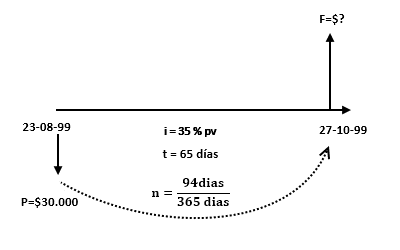
\includegraphics[height=5cm]{1_2}
\end{center}

b. Declaración de variables

%\begin{align*}
F=\$? \\ P=\$30.000 \\ i=35\% pdv \\ t=65 días\\ $n=\frac{65}{365}$ pdv
%\end{align*}

c. Declaración de fórmulas

\begin{align*}
F=P(1+in) \hspace{35 pt} \textit{Valor futuro}
\end{align*}

d. Desarrollo matemático

\begin{align*}
F=\$30.000(1 + 0,35\frac{65}{365})= \$31.869,86 \hspace{35 pt} \textit{Ecuación de valor}
\end{align*} \hspace{35 pt} 

e. Respuesta:
\\
Luego el valor final (F) es de \$31.869,86

\section{Capital inicial (P, i, n, F)}
Si despejamos P de la fórmula del monto se tiene una fórmula equivalente que nos permite calcular el valor inicial o valor presente:

\begin{align*}
	P=\frac{F}{1+in} \hspace{35 pt} \textit{Valor presente}
\end{align*}

\textbf{Ejemplo 2}
\\
¿Cuánto dinero debo depositar hoy 25 de abril en una cuenta que paga el 23\% período año vencido para que el 28 de julio pueda retirar \$60.000? Utilice año de 365 días.
\\\\
\textbf{Solución:}
\\
\textbf{a.}	Diagrama de flujo
\begin{center}
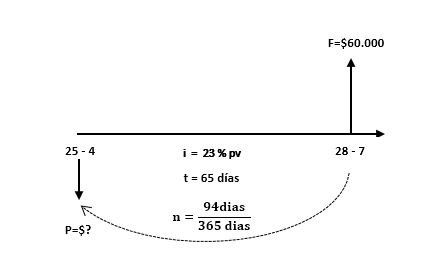
\includegraphics[height=5.1cm]{1_3}
\end{center}

\textbf{b.} Declaración de variables: \\
%\begin{align*}
P=\$?\\
F=\$60.000\\ 
$n=\frac{(94)}{(365}$pdv \\
i=23\% pdv
%\end{align*}

\textbf{c.} Declaración de formulas
\begin{align*}
P=\frac{F}{1+in} \hspace{35 pt} \textit{Valor presente de un flujo futuro (F)}
\end{align*}

\textbf{d.} Desarrollo matemático
\begin{align*}
P=\frac{\$60.000}{1+0,23  \frac{94}{365}} \hspace{35 pt} \textit{Ecuación de valor}
\end{align*}

\textbf{e.} Respuesta
El dinero que se debe depositar (P) es de \$56.644,77, \\
Justifiación: el valor Presente (p) es menor, en  valor absoluto, que el valor F de \$60.000, sin embargo estas dos sumas son equivalentes en el tiempo. 
\\\\
\textbf{Ejemplo 3}
\\
¿A qué tasa perió dica vencida, \$30.000 se convertirán en \$35.000 en 6 meses?
\\\\
\textbf{Solución:}
\\
\textbf{a.} Diagrama de flujo
\begin{center}
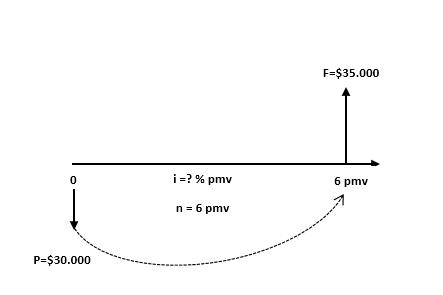
\includegraphics[height=5.1cm]{1_4}
\end{center}

\textbf{b.} Declaración de variables: \\

F=\$35.000\\
P=\$30.000 \\
i=\%? pmv\\
n=6 pmv\\


\textbf{c.} Declaración de formulas
\begin{align*}
F=P(1+in) \hspace{35 pt} \textit{Valor futuro }
\end{align*}

\textbf{d.} Desarrollo matemático
\\
despejando i:
\begin{align*}
i=\frac{F}{nP}-\frac{1}{n}=\frac{\$35.000}{(6 x \$30.000)}-\frac{1}{6}=0,3333 \Leftrightarrow 33,33\% pmv \  \hspace{35 pt} \textit{Ecuación de valor}
\end{align*}

\textbf{e.} Respuesta \\
Los \$30.000 se convertirán en \$35.000 a los 6 meses con una tasa periódica vencida de 33,33\% pmv. 

\section{Interés anticipado (I$_{a}$)}
El Interés anticipado consiste en cobrar los intereses al principio del período.

\section{Tasa anticipada (d)}
La tasa anticipada es la que genera el interés anticipado y la representaremos por $"d"$, como veremos más adelante también se le denomina tasa de descuento.

\section{Descuento simple (D)}
El descuento simple consiste en cobrar intereses por anticipado calculados sobre el valor final.
\\\\
Ya vimos que la fórmula del interés simple vencido es $I= P i n$ y por similitud, la fórmula del descuento que corresponde al interés simple anticipado será:
\begin{center}
$D=Fdn$ \hspace{35 pt} \textit{Valor de descuento}
\end{center}
Donde $D$ es la cantidad descontada.

\section{Valor líquido (VL)}
Se denomina valor líquido, valor de transacción, valor presente, valor actual o monto al valor nominal menos el descuento. De acuerdo con esta definición la fórmula del valor líquido será:
\begin{center}
$VL=F(1-dn)$ \hspace{35 pt} \textit{Valor líquido dado un flujo futuro (F)}
\end{center}

\textbf{Ejemplo 4}
\\
Supongamos que el 17 de abril de 1999 una persona necesita comprar mercancías por valor de \$800.000 para surtir su almacén y además solicita a la fábrica un plazo de 3 meses para el pago de la factura. Naturalmente que la fábrica está interesada en hacer la venta y para ello le otorgará un crédito pero le exige un documento como seguridad del pago de la deuda a su vencimiento; éste puede ser una letra que quedará en poder de la fábrica y será cobrada a su vencimiento.
\\\\
Los \$800.000 constituyen el valor nominal de la letra que tendrá por vencimiento el 17 de julio del mismo año.
\\\\
Ahora supongamos que el 20 de junio a la fábrica se le presentó un gasto inesperado y que necesita dinero en efectivo para cubrir esta contingencia; la fábrica puede ir al banco ABC a ofrecerle en venta la letra, pero es obvio que el banco no le pagará \$800.000 por el documento sino que sobre el valor nominal hará un descuento, es decir que cobrará una tasa de descuento (d).
\\\\
Ahora supongamos que el banco ABC en este tipo de operaciones cobra una tasa de descuento (d) del 36\% simple anticipado.
\\\\
¿Cuál es el valor presente de la letra, esto es cual es valor que el banco paga a la fábrica? Utilice año de 360 días.
\\\\
\clearpage
\textbf{Solución:}
\\
Entonces el primer paso para calcular el descuento será hallar los días de diferencia entre esas dos fechas.
\begin{center}
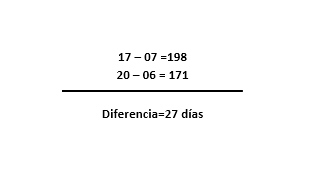
\includegraphics[height=4cm]{1_5}
\end{center}
Continuando con el problema, la gráfica de flujo de caja se presenta a continuación:
\\\\
\textbf{a. }Diagrama de flujo (del banco):
\begin{center}
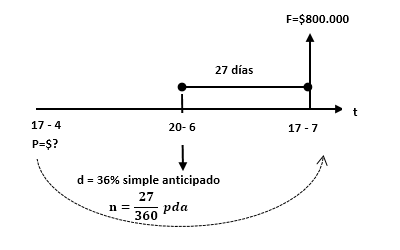
\includegraphics[height=5.1cm]{1_6}
\end{center}

\textbf{b.} Declaración de variables: \\
%\begin{align*}
P=\$?\\
F=\$800.000\\
d = 36\% simple anticipado\\
$n=\frac{27}{360}$ pda
%\end{align*}

\textbf{c.} Declaración de formulas:
\begin{align*}
VL= F(1-dn) \hspace{35 pt} \textit{Valor líquido dado un flujo futuro (F)}\\
\end{align*}

\textbf{d. }Desarrollo matemático
\begin{align*}
VL=\$800.000(1-\frac{0.36x27}{360})  = \$778.400 \hspace{35 pt} \textit{Ecuación de valor}
\end{align*}

\textbf{e.} Respuesta, el banco pagará a la fábrica la suma de \$778.400
\\\\
\textbf{Ejemplo 5}
¿Cuál debe ser el valor nominal de un documento que va a ser descontado (d) por un banco al 38\% simple anticipado entre el 17 de diciembre de 1998 y el 25 de enero de 1999 si el valor de negociación (P) es de \$637.437? Utilice año de 360 días.
\\\\
\textbf{Solución:}
calculamos los días que hay entre esas dos fechas los cuales vienen a ser 39 días.
\\
\textbf{a.} Diagrama de flujo
\begin{center}
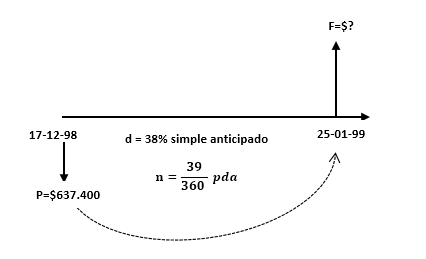
\includegraphics[height=6cm]{1_7}
\end{center}

\textbf{b. }Declaración de variables \\
%\begin{align*}
F=\$?\\
P=\$637.400\\
d=38\%\ pda\\
$n=\frac{39}{360}$pda
%\end{align*}

\textbf{c.} Declaración de formulas
\begin{align*}
P=F(1-dn) \hspace{35 pt} \textit{Valor presente de un flujo futuro (F)}\\
F=P/(1-dn) \hspace{35 pt} \textit{Valor futuro de un flujo presente (P)}\\
\end{align*}

\textbf{d.} Desarrollo matemático
\begin{align*}
F=\frac{\$637.437}{(1-0.37  \frac{39}{360})} \hspace{35 pt} \textit{Ecuación de valor}
\end{align*}

\textbf{e.} Respuesta
\\
En consecuencia el valor nominal del documento debe ser 
\$664.804,80


\section{Tasa realmente cobrada en una operación de descuento (i\%)}$(Equivalencia\  con\ la\  tasa\  de\  descuento\  [d]\  a\  la\  tasa\  de\  inter\acute{e}s\  (i\%))$


La tasa de descuento se aplica al valor final del documento, pero la tasa de interés (i\%) se aplica al valor inicial. Para calcular la tasa que realmente se cobra en una operación de descuento se aplica la fórmula del valor futuro (F).

\begin{center}
$F=P(1+in)$ \hspace{35 pt} \textit{Valor futuro}
\end{center}

\textbf{Ejemplo 6}
Una letra por valor de \$600.000 va a ser descontada por un banco 35 días antes del vencimiento al 38\%  simple anticipado. Calcular la tasa de interés periódica vencida. Utilice año de 360 días.
\\\\
\textbf{Solución}\\
\textbf{a.} Diagrama de flujo
\begin{center}
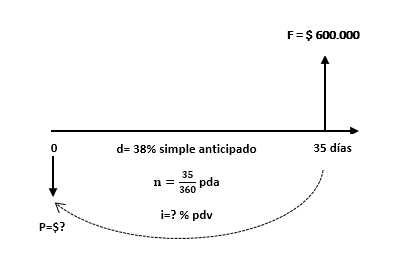
\includegraphics[height=6cm]{1_8}
\end{center}
\textbf{b.} Declaración de variables \\
%\begin{align*}
F=\$600.000\\
P=\$ ?\\
d=38\% \ da
%\end{align*}

\textbf{c.} Declaración de formulas\\
\begin{align*}
P=F(1-dn) \hspace{35 pt} \textit{Valor presente} \\
F=P(1+in)\hspace{35 pt} \textit{Valor futuro}\\
\end{align*}

\textbf{d.} Desarrollo matemático\\
\\
Igualando P de las fórmulas declaradas en el item anterior se tiene que:
P 
\begin{align*}
P=VL=\$600.000(1-0.38  \frac{35}{360})=\$577.833,33
\end{align*}
Observamos que hoy el banco invierte \$577.833,33 y a los  35 días obtiene \$600.000

\textbf{e.} Respuesta
\\
Despejando se tiene que i = 39,46\% p(35)dv
\\\\
\textbf{f.} Justificación
\\
La tasa de interés periódica y la tasa de descuento simple son equivalentes porque parten del mismo valor presente y valor futuro. Sin embargo, en términos absolutos la tasa de interés real es mayor que la tasa de descuento porque parte del valor presente (P), valor absoluto inferior del valor futuro (F).

\section{Descuentos en cadena}
Es usual que sobre una misma factura ocurran varios descuentos, tal es el caso cuando una fábrica vende mercancía a un almacén, en este caso la fábrica ofrece una serie de descuentos que son aplicables a la misma factura. Tales descuentos pueden ser:


\subsection{Descuento por volumen}
Consiste en otorgar un descuento que será progresivo conforme al valor de la factura, (en ocasiones el descuento se otorga con base en el número de unidades vendidas).

Este tipo de descuento intenta incentivar al comprador para que haga un pedido mayor con lo cual sus ganancias aumentarán al tener un mayor descuento Un ejemplo de tabla de descuento al por mayor puede ser la siguiente:

\begin{table}[H]
\fontsize{11}{9}\selectfont
\centering
\label{Descuento por volumen}
\begin{tabular}{|l|l|c|l|}
\hline
\multicolumn{2}{|c|}{Valor de la factura}                 & \multicolumn{2}{c|}{Descuento} \\ \hline
\multicolumn{2}{|c|}{Menor de \$100.000}                  & \multicolumn{2}{c|}{0\%}       \\ 
\multicolumn{2}{|c|}{Más de \$100.000 y menos de \$200.000} & \multicolumn{2}{c|}{10\%}      \\ 
\multicolumn{2}{|c|}{Más de \$200.000 y menos de \$300.000} & \multicolumn{2}{c|}{15\%}      \\
\multicolumn{2}{|c|}{Más de \$300.000 y menos de \$400.000} & \multicolumn{2}{c|}{20\%}      \\ 
\multicolumn{2}{|c|}{Más de \$400.000 y menos de \$500.000} & \multicolumn{2}{c|}{25\%}      \\
\multicolumn{2}{|c|}{Más de \$500.000}                    & \multicolumn{2}{c|}{30\%}      \\ \hline
\end{tabular}
\caption{Descuentos por volumen}
\end{table}

\subsection{Descuento por pronto pago}
Tiene por objeto incentivar al comprador a que pague lo más pronto posible, el descuento estará en relación inversa con el plazo para pagar la factura, un ejemplo de tabla puede ser:

\begin{table}[H]
\fontsize{11}{9}\selectfont
\centering
\label{Descuento por pronto pago}
\begin{tabular}{|c|l|c|l|}
\hline
\multicolumn{2}{|c|}{Plazo}      & \multicolumn{2}{c|}{Descuento} \\ \hline
\multicolumn{2}{|c|}{Al contado} & \multicolumn{2}{c|}{10\%}      \\ 
\multicolumn{2}{|c|}{30 días}    & \multicolumn{2}{c|}{6\%}       \\ 
\multicolumn{2}{|c|}{60 días}    & \multicolumn{2}{c|}{3\%}       \\ 
\multicolumn{2}{|c|}{90 días}    & \multicolumn{2}{c|}{0\%}       \\ \hline
\end{tabular}
\caption{Descuento por pronto pago}
\end{table}

\subsection{Descuento por no embalaje}
Hay almacenes que venden la mercancía empacada con el logotipo del fabricante; en ocasiones hacen el pedido y solicitan que llegue sin empacar, entonces la fábrica concede un descuento adicional igual al costo del empaque, otras veces puede ser que la mercancía llegue con un empaque más económico que el normal, o con un empaque de lujo el cual tendrá un recargo.

\subsection{Descuento por temporada}
A fin de incentivar las ventas en épocas de baja demanda las fábricas ofrecen un descuento adicional para los pedidos que sean cancelados dentro de ciertas fechas. 

\subsection{Descuento por fidelidad}
También se conoce con el nombre de descuento por antigüedad, es un pequeño porcentaje que se otorga a los clientes más leales.
\\\
Las anteriores son las principales razones para otorgar descuentos, sin embargo estos nunca se suman unos con otros sino que una vez que se aplicó el primero al saldo de la factura se le aplica el siguiente descuento y así sucesivamente hasta agotarlos todos; la respuesta final no varía si se cambia el orden de aplicar los descuentos según se puede deducir del siguiente análisis.

El descuento total será el valor nominal de la factura menos el valor de cancelación de la factura, esto es:

\begin{center}
$D=F-F(1-d_{1} )(1-d_{2} )...(1-d_{n})$

\end{center}

Esta fórmula se demuestra a través de la siguiente tabla: \\ \\

\begin{center}
\begin{table}[H]
\fontsize{11}{9}\selectfont
\centering
\begin{tabular}{@{}|c|c|c|c|@{}}
\toprule
\textbf{\begin{tabular}[c]{@{}c@{}}Valor de la Factura\\ antes del Descuento\\ {[}F{]}\\ (1)\end{tabular}} & \textbf{\begin{tabular}[c]{@{}c@{}}Tasa de \\ Descuento\\ {[}d{]}\\ (2)\end{tabular}} & \textbf{\begin{tabular}[c]{@{}c@{}}Valor del\\ Descuento\\ {[}D=Fd{]}\\ (3)\end{tabular}} & \textbf{\begin{tabular}[c]{@{}c@{}}Valor de la factura\\ después del descuento\\ {[}P = F-D = F - F  d{]}\\ (4)\end{tabular}} \\ \midrule
F                                                                                                          & $d_1$                                                                                  & $Fd_1$                                                                                      & $F-Fd_1 = F(1-d_1)$                                                                                                            \\
$F(1-d_1)$                                                                                                  & $d_2$                                                                                 & $F(1-d_1)d_2$                                                                              & \begin{tabular}[c]{@{}c@{}}$F(1-d_1) - F(1-d_1)d_2 \\= F(1-d_1)(1-d_2)$\end{tabular}
                                                                                  \\
$F(1-d_1)(1-d_2)$                                                                                          & $d_3$                                                                                  & $F(1-d_1)(1-d_2)d_3$                                                                     & \begin{tabular}[c]{@{}c@{}}$F(1-d_1)(1-d_2)-F(1-\\d_1)(1-d_2)d_3 =  F(1-d_1)(1-\\d_2)(1-d_3)$\end{tabular}                 \\
|                                                                                                          & |                                                                                     & |                                                                                          & |                                                                                                                              \\
|                                                                                                          & |                                                                                     & |                                                                                          & |                                                                                                                              \\
|                                                                                                          & |                                                                                     & |                                                                                          & |                                                                                                                              \\
|                                                                                                          & |                                                                                     & |                                                                                          & |                                                                                                                              \\

\begin{tabular}[c]{@{}c@{}}$F(1-d_1)(1-d_2)...(1-\\d_{n-1})$  \end{tabular}& $d_n$                                                                                  & \begin{tabular}[c]{@{}c@{}}$F(1-d_1)(1-d_2)...(1-\\d_{n-1})d_n$  \end{tabular}
                                                       & $F(1-d_1)(1-d_2)...(1-d_n)$                                                                                                   \\ \bottomrule
\end{tabular}
\end{table}
\end{center}


%----------------------------------------------------------------------------------------
%	INDEX
%----------------------------------------------------------------------------------------

\cleardoublepage
\phantomsection
\setlength{\columnsep}{0.75cm}
\printindex


%----------------------------------------------------------------------------------------




\part{Capítulo dos}
\graphicspath{ {img/ch2/}, {img/} }

%----------------------------------------------------------------------------------------
%	CHAPTER 2
%----------------------------------------------------------------------------------------

\chapterimage{ima2} % Chapter heading image

\chapter{Interés compuesto}
%---------------------------------
%Tabla de fòrmulas
%------------------------------------------

\section{{Fórmulas del capítulo}}

\begin{spacing}{1.5}
\begin{center}
\begin{tabular}{ |p{6cm}|p{5cm}| p{4cm}|}
\hline 
\rowcolor{orange!50}
\begin{center}\textbf{Fórmula} \end{center} & \begin{center} \textbf{Nombre}\end{center} &  \begin{center} \textbf{Excel} \end{center} \\ \hline                       



F = $P(1+i)^n$ & Valor futuro & VF(i;n;;VA,0)\\ \hline

j = im & Tasa nominal anual & TASA.NOMINAL(i;m) \\ \hline

P = $\frac{F}{(1 + i)^{n}}$ &   Valor presente & VA(i;n;;VF,0)\\ \hline

${(1 + i_{1})^{n}}$ = ${(1 + i_{2})^{n}}$ &   Equivalencia de tasas & TASA(m;;-1;1+i)\\ \hline
 
\end{tabular}
\end{center}
\end{spacing}
\section{Interés compuesto}
Es el retorno de una inversión producto de la capitalización o acumulación de intereses generados por un capital en un período determinado de tiempo.\\

\textbf{Ejemplo 1:}\\
Supongamos que tenemos un capital de \$1.000 que será invertido al 10\% periódico trimestre vencido, durante un año. Use año de 360 días.\\

A. Calcular el valor total de los intereses simples si son cancelados cada trimestre\\
B. Si son capitalizados y cancelados al final del tiempo de la inversión.\\

\textbf{Solución:}\\

A. Cálculo de interés simple, pagado trimestre vencido.\\
\begin{itemize}
	\item a. Diagrama de flujo de caja:\\
	
	\begin{center}
		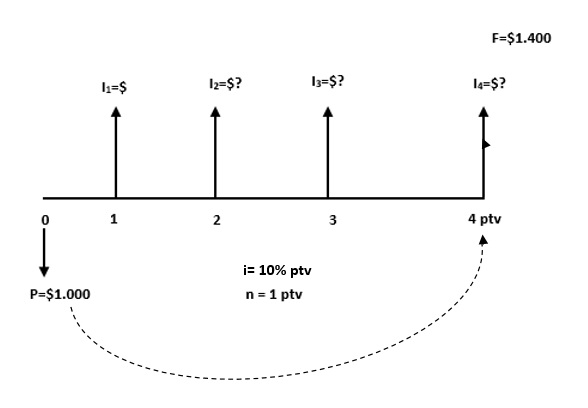
\includegraphics[height = 5.1 cm]{2_1}\\
	\end{center}
	
	\begin{table}[]
\centering
\label{my-label}
\begin{tabular}{|c|c|c|c|}
\hline
\begin{tabular}[c]{@{}c@{}}Periodo\\ {[}1{]}\end{tabular} & \begin{tabular}[c]{@{}c@{}}Capital Inicial (P) \\ {[}2{]}\end{tabular} & \begin{tabular}[c]{@{}c@{}}Interes simple (I)\\ {[}3{]}\end{tabular} & \begin{tabular}[c]{@{}c@{}}Capital final (F) \\ {[}4{]}\end{tabular} \\ \hline
0                                                         & \$1.000                                                                & 0                                                                    & \$1.000                                                              \\ \hline
1                                                         & \$1.000                                                                & \$100                                                                & \$1.100                                                              \\ \hline
2                                                         & \$1.000                                                                & \$100                                                                & \$1.200                                                              \\ \hline
3                                                         & \$1.000                                                                & \$100                                                                & \$1.300                                                              \\ \hline
4                                                         & \$1.000                                                                & \$100                                                                & \$1.400                                                              \\ \hline
\end{tabular}
\end{table}
	
    \item b. Declaración de variables:\\
	
	i= 10\% ptv\\
	n = $\frac{90\ d\acute{i}as}{90\ d\acute{i}as} = 1 ptv $\\
	
	\item c. Declaración de fórmulas:\\
	I=Pin \hspace{35 pt}  \textit{Interés monetario simple}\\
	
	\item d. Desarrollo matemático:\\
	I$_{1}$ = \$1.000x0,1x1\\
	I$_{1}$ = \$100\\
	
	I = 4x\$100\\
	I = \$400\\
	
	VF = P + 4I\\
	VF = \$1.400\\
	
	\item e. Respuesta\\
El valor de los intereses simples es:	I = \$400\\
	
\end{itemize}

B. Calculo de I al final del tiempo de la inversión capitalizando los intereses.\\


\begin{itemize}
	\item a. Diagrama de flujo de caja:
	
	\begin{center}
		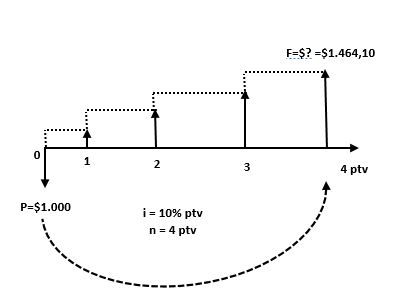
\includegraphics[height = 5.1 cm]{2_2}\\
	\end{center}
	
	\item b. Declaración de variables:\\
	
	i = 10\% ptv\\
	t = 360 días\\
	n = $\frac{360\ dias}{90\ dias} = 4 ptv$ \\
	
	\item c. Declaración de fórmulas:\\
	I= Pin \hspace{35 pt}  \textit{Interés monetario simple}\\
	Calculando para n= 1 ptv y capitalizando los intereses.\\
	
	\item d. Desarrollo matemático:
	
    \begin{table}[]
\centering
\label{my-label}
\begin{tabular}{|c|c|c|c|}
\hline
\begin{tabular}[c]{@{}c@{}}Periodo\\ {[}1{]}\end{tabular} & \begin{tabular}[c]{@{}c@{}}Capital Inicial (P) \\ {[}2{]}\end{tabular} & \begin{tabular}[c]{@{}c@{}}Interes simple (I)\\ {[}3{]}\end{tabular} & \begin{tabular}[c]{@{}c@{}}Capital final (F ó S) \\ {[}4{]}\end{tabular} \\ \hline
0                                                         & \$1.000                                                                & 0                                                                    & \$1.000                                                                  \\ \hline
1                                                         & \$1.000                                                                & \$100                                                                & \$1.100                                                                  \\ \hline
2                                                         & \$1.100                                                                & \$110                                                                & \$1.210                                                                  \\ \hline
3                                                         & \$1.210                                                                & \$121                                                                & \$1.331                                                                  \\ \hline
4                                                         & \$1.331                                                                & \$133,10                                                             & \$1.464,10                                                               \\ \hline
\end{tabular}
\end{table}
	
	\item e. Respuesta:\\
	
	I= \$ 464,10\\
\end{itemize}

\textbf{Generalizando se tiene que:}\\

Algebráicamente se puede representar el resultado anterior de la siguiente forma:\\


Con lo que llegamos a concluir que la fórmula del interés compuesto es:

	$F = P(1+i)^n$ \hspace{35 pt} \textit{Valor futuro}\\ 

\begin{table}[]
\centering
\label{my-label}
\begin{tabular}{|c|c|c|c|}
\hline
\textbf{\begin{tabular}[c]{@{}c@{}}Período (n)\\ {[}1{]}\end{tabular}}    & \textbf{\begin{tabular}[c]{@{}c@{}}Capital inicial (P)\\ {[}2{]}\end{tabular}}                     & \textbf{\begin{tabular}[c]{@{}c@{}}Interés (I)\\ {[}3{]}\end{tabular}}                                  & \textbf{\begin{tabular}[c]{@{}c@{}}Capital final (F)\\ {[}4{]}\end{tabular}}                                                                                                                                                       \\ \hline
\begin{tabular}[c]{@{}c@{}}0\\ 1\\ 2\\ 3\\ 4\\ .\\ .\\ .\\ n\end{tabular} & \begin{tabular}[c]{@{}c@{}}0\\ P\\ P(1+i)\\ $P(1+i)^{2}$\\ $P(1+i)^{3}$\\ .\\ .\\ .\\ $P(1+i)^{n-1}$\end{tabular} & \begin{tabular}[c]{@{}c@{}}0\\ Pi\\ P(1+i)i\\ $P(1+i)^{2}i$\\ $P(1+i)^{3}i$\\ .\\ .\\ .\\ $P(1+i)^{n-1}i$\end{tabular} & \begin{tabular}[c]{@{}c@{}}$F_{0}$ = P\\ $F_{1}$ = P + Pi = P(1+i)\\ $F_{2}$ = P(1+i) + P(1+i)i = $P(1+i)^{2}$\\ $F_{3}$ = $P(1+i)^{2}$ +$P(1+i)^{2}i$ = $P(1+i)^{3}$\\ $F_{4}$ = $P(1+i)^{3} + P(1+i)^{3}i = P(1+i)^{4}$\\ .\\ .\\ .\\ $F_{n} = P(1+i)^{n-1} + P(1+i)^{n-1}i = P(1+i)^{n}$\end{tabular} \\ \hline
\end{tabular}
\end{table}

\textbf{Volviendo al ejemplo 1:}\\

$F = P(1+i)^n$\\ 
$F = \$1.000 (1+0,1)^4$\\
$F = \$1.460,10$\\

C. ¿A qué tasa de interés periódica año vencido [$i_{2}$] es equivalente la tasa de interés del 10\% periódica trimestre vencido [$i_{1}$], del ejemplo anterior? Y calcule la tasa efectiva anual vencido de referencia.\\

\begin{itemize}
	\item a. Diagrama de flujo de caja:\\
	\begin{center}
		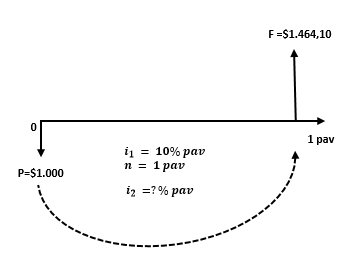
\includegraphics[height = 5.5 cm]{2_5}\\
	\end{center}
	
	\item b. Declaración de variables:\\
	
	i = ? \% pav\\
	t = 360 días\\
	P = \$1.000\\
	F = \$1.464,10\\
	n = $\frac{360 d\acute{i}as}{360 d\acute{i}as}$ = 1 pav\\
	
	\item c. Declaración de fórmulas:\\
	
	$VF = P(1+i)^n$ \hspace{35 pt} \textit{Valor futuro}
	
	\item d. Desarrollo matemático:\\
	
	\$1.464,10 = $\$1.000(1+i)^1$ \hspace{35 pt} \textit{Ecuación de valor}\\
	
	$\frac{\$1.464,10}{\$1.000} - 1 = i$\\
	
	i = 0,4641 pav\\
	
	\item e. Respuesta:\\
	
	i=46,41\%  pav\\
	j = im Tasa nominal anual\\
    $j = 46,41$ \%$ x 1 $pav $= 46,41$\ naav\Leftrightarrow  $46,41$\% EA\ 
	
	\textbf{Equivalente a:}\\
	j = i  m\\
	j = 10\% ptv x 4 ptv = 40\% natv\\
	j = 40\% natv\\
	
	\textbf{IMPORTANTE:} $40\% natv \equiv 46,4\% naav \equiv 46,4\% EA$\\
	
\end{itemize}

\textbf{Equivalencias de tasa de interés de 40\% natv con 46\% EA:}\\

%\usepackage{multirow}
\begin{table}[]
\centering
\label{my-label}
\begin{tabular}{|c|c|c|c|}
\hline
\textbf{Período trimestral} & \textbf{Capital} & \textbf{Interés} & \textbf{Tasa nominal}                            \\ \hline
0                           & \$100,0          & \$0,0            & \multirow{5}{*}{\textit{\textbf{j = 40\% natv}}} \\ \cline{1-3}
1                           & \$110,0          & \$10,0           &                                                  \\ \cline{1-3}
2                           & \$121,0          & \$11,0           &                                                  \\ \cline{1-3}
3                           & \$133,1          & \$12,1           &                                                  \\ \cline{1-3}
4                           & \textbf{\$146,4} & \$13,3           &                                                  \\ \hline
\end{tabular}
\end{table}

% \usepackage{multirow}
\begin{table}[]
\centering
\label{my-label}
\begin{tabular}{|c|c|c|c|}
\hline
\textbf{Período anual} & \textbf{Capital} & \textbf{Interés} & \textbf{\begin{tabular}[c]{@{}c@{}}Tasa nominal \equiv EA \\ \equiv Efectiva anual\end{tabular}} \\ \hline
0                      & \$100,0          & \$0,0            & \multirow{2}{*}{\textit{\textbf{j = 46,4\% naav}}}                                     \\ \cline{1-3}
1                      & \$146,4          & \$46,4           &                                                                                        \\ \hline
\end{tabular}
\end{table}

\section{Tasa de interés periódica (i)}

Es la expresión porcentual del interés aplicada a un capital en un período (por ejemplo diario, mensual, bimestral, trimestral, semestral, anual, bianual, etc..). Se representa por i.\\

\textbf{Tasa de interés nominal anual [j]}\\

Corresponde a la anualización de tasa periódica (i):\\

j = im ; En donde m = número de períodos de la tasa periódica.\\

$i = \frac{j}{m}$ \hspace{2 cm} \\

\textbf{Del ejemplo 1:}\\

i = 10\%  ptv\\
m = 4 ptv\\
j = i  m\\
j = 10\% x 4 ptv\\
j = 40\% natv\\

\textbf{Ejemplo 2}\\

Calcular la tasa periódica semestral vencida a partir del 28\% nominal anual semestre vencido. \\
\begin{itemize}
	
	\item a. Declaración de variables:\\
	
	j = 28\% nasv\\
	i = ?\% psv\\
	
	\item b. Declaración de fórmulas:\\
	
	j = im  \hspace{35 pt} \textit{Tasa de interés nominal}
	
	\item c. Desarrollo matemático:\\
	
	$i = \frac{28\%}{2} psv = 14\% $ psv\\
	
	\item e. Respuesta:\\
	
	i = 14\% psv\\
	
\end{itemize}

\textbf{Ejemplo 3}\\

Se invierte \$200.000 en un depósito a término fijo de 6 meses en un banco que paga el 28,8\% namv determinar el monto de la entrega al vencimiento.\\

\begin{itemize}
	\item a. Diagrama de flujo de caja:\\
	
	\begin{center}
		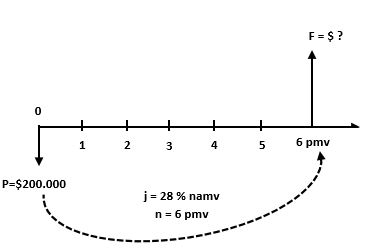
\includegraphics[height = 5.5 cm]{2_7}\\
	\end{center}
	
	\item b. Declaración de variables\\
	
	n = 6 pmv\\
	j = 28,8\% namv\\
	m = 12 pmv\\
	P = \$200.000\\
	F = \$?\\
	\item c.Declaración de fórmulas:\\
	
	$j = im$ \hspace{35 pt} \textit{Tasa de interés nominal anual vencida}\\
	
	$F = P(1+i)^n$ \hspace{35 pt} \textit{Valor futuro dado un valor presente}\\
	
	\item d. Desarrollo matemático:\\
	
	$i = \frac{28\%}{12} = 0,024$ pmv\\	
	$F = \$200.000 (1+0,024)^6$ \hspace{35 pt} \textit{Ecuación de valor} \\
	$F = \$230.584,30$\\
	
	\item e. Respuesta: \\
	
	$F = \$230.584,30$\\
	
\end{itemize}

\textbf{Ejemplo 4}\\

Una persona debe cancelar la suma de \$ 2'000.000 al cabo 18 meses. ¿Cuál debe ser el valor del ahorro que debe hacer hoy en una cuenta que paga el equivalente al 32\% nominal anual trimestre vencido para poder cancelar la deuda?\\

\begin{itemize}
	\item a. Diagrama de flujo de caja de la persona:\\
	\begin{center}
		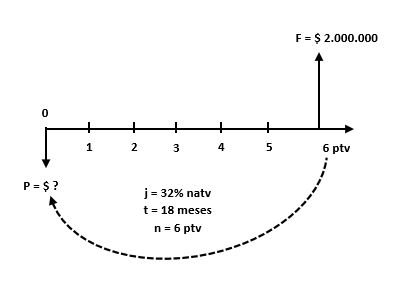
\includegraphics[height = 5.3 cm]{2_8}\\
	\end{center}
	
	\item b. Declaración de variables:\\
	
	t = 18 meses\\
	\\
	$n = \frac{18 meses}{3 meses}$ = 6 ptv\\
	\\
	j=32\% natv\\
	\\
	i=  $\frac{32\% natv}{4 ptv}$\\
	\\
	i = 8\% ptv\\
	\\
	F = \$ 2'000.000\\
	\\
	P = \$?\\
	
	\item c. Declaración de fórmulas:\\	
	F = $ P(1 + i)^n$ \hspace{35 pt} \textit{Valor futuro dado un valor presente}
	
	P = $\frac{F}{(1 + i)^{n}}$ \hspace{35 pt} \textit{Valor presente dado un valor futuro}\\	
	\item d. Desarrollo matemático:\\
	
	P = $\frac{\$2'000.000}{(1 + 0,08)^6}$ \hspace{35 pt} \textit{Ecuación de valor}\\
	
	P =  \$1'260.339,25\\
	
	\item e. Respuesta:\\
	
	P =  \$1'260.339,25\\ 
\end{itemize}

\textbf{Ejemplo 5}\\

¿A qué tasa nominal anual mes vencido se triplica un capital en $2^{\frac{1}{2}}$ años?\\

\begin{itemize}
	\item a. Diagrama de flujo de caja:\\
	\begin{center}
		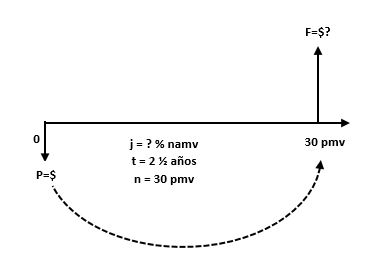
\includegraphics[height = 5.3 cm]{2_9}\\
	\end{center}
	
	\item b.Declaración de variables\\
	
	t = $2^{\frac{1}{2}}$ años\\
	n = 30 pmv\\
	j = ? \% namv \\
	m = 12 pmv\\
	P = ? \\
	F = ? \\
	
	\item c. Declaración de fórmulas:\\
	
	F = $ P(1 + i)^n$ \hspace{35 pt} \textit{Valor futuro}\\
	
	j = im \hspace{35 pt} \textit{Tasa nominal anual}\\
	
	\item d. Desarrollo matemático:\\
	
	\$3 = \$1 $(1 + i)^{30}$ \hspace{35 pt} \textit{Ecuación de valor}\\
	
	$\frac{\$3}{\$1}^{\frac{1}{30}} - 1$ = i\\
	
	i = 0,0373 pmv\\
	i = 3,73\% pmv\\
	
	Equivalente a:\\
	
	j = 3,73\%pmv x 12\%pmv\\
	j = 44,76\% namv\\
	
	\item e. Respuesta:
	
	j = 44,76\% namv\\
	
\end{itemize}

\textbf{Ejemplo 6}

¿En cuánto tiempo se duplica un capital a una tasa del 24\% nominal anual mes vencido?\\

\begin{itemize}
	\item a. Diagrama de flujo de caja:\\
	\begin{center}
		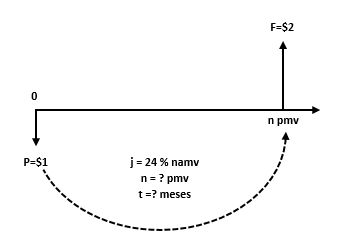
\includegraphics[height = 5.3 cm]{2_10}\\
	\end{center}
	\item b. Declaración de variables:\\
	
	j = 24\% namv\\ % \hspace{1 cm} i = 2\% pmv\\
	n = ? pmv\\
	P = 1\$\\
	F = 2\$\\
	t = ?\$ meses\\
	
	\item c. Declaración de fórmulas:\\
	
	j = im \hspace{35 pt} \textit{Tasa nominal anual}\\
	
	F = $ P(1 + i)^n$ \hspace{35 pt} \textit{Valor futuro}\\
	
	\item d. Desarrollo matemático:\\
	
	$i= \frac{0,24 namv}{12 pmv}$\\

	i= 0,02 pmv\\
	
	\$2 = \$1 $(1+0,02)^n$ \hspace{35 pt} \textit{Ecuación de valor}\\
	log2 = nlog(1,02)\\
	
	n = $\frac{log2}{log(1,02)} = 35$ pmv\\
	
	$n = 35 pmv \equiv t=35 meses$\\
	
	
	\item e. Respuesta:\\
	
	n = 35 pmv\\
	t = 35 meses\\
	
\end{itemize}

\section{Equivalencia de tasas ($i_{1} \equiv i_{2}$)}

Tasas equivalentes de interés son aquellas que teniendo diferente periodicidad y/o modalidad de liquidación de intereses producen el mismo monto al final o al comienzo del flujo.\\

\textbf{Ejemplo 7}\\

¿A qué tasa de interés periódica semestre vencido se debe invertir un capital para que el valor al vencimiento de un año sea igual a la misma inversión a una tasa periódica del 10\% periodo trimestre vencido?¿Cuál es el valor final  de \$100 al 10\% ptv= ? 
\begin{itemize}
	\item a. Diagrama de flujo de caja:
	
	\begin{center}
		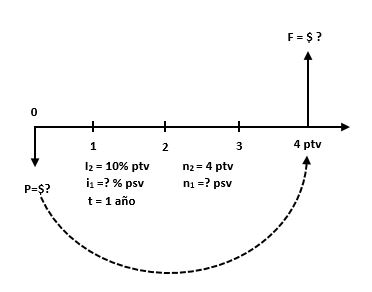
\includegraphics[height = 5.3 cm]{2_11}\\
	\end{center}
	
	\item b. Declaración de variables:\\ \\
	
	
	
	$i_{2}$ = 10\% ptv \\
	$m_{2}$ = 4 ptv\\
	t = 1 año\\
	$i_{1}$ = ? \% psv \\
	$m_{1}$ = 2 psv\\
	P = \$100\\
	F = \$?\\
	 
	
	\item c. Declaración de fórmulas:\\
	
	
	$(1+i_{1})^{m_{1}}$ = $(1+i_{2})^{m_{2}}$ \hspace{35 pt} \textit{Equivalencia de tasas}\\
    F = $ P(1 + i)^n$ \hspace{70 pt} \textit{Valor futuro dado un valor presente}\\
	\item d. Desarrollo matemático:\\
	
    $(1+i_{1})^{2} = (1+0,1)^{4}$\\
    
    $i_{1} = 21$ \% psv \\  
	 	
	
	   F= $\$100 (1 + 0,1)^{4}$ \\
       F = \$146,41
       
 \item e. Respuesta:\\
	
	i$_{1}$ = 21 \% psv \\
	F = \$146,41 \\\\
	
	
\end{itemize}

\textbf{Ejemplo 8}\\

Dado el 5\% período bimestre vencido, calcular una tasa periódica trimestral vencido.\\

\begin{itemize}
	\item a. Declaración de variables:\\
	
	$i_{1}$ = 5\% pbv\\
	$m_{1}$ = 6 pbv\\
	$i_{2}$ = ?\% ptv\\
	$m_{2}$ = 4 ptv\\
	
	\item b. Declaración de fórmulas:\\
	
	$(1+i_1)^{m_1} = (1+i_2)^{m_2}$ \hspace{35 pt} \textit{Equivalencia de tasas}\\
	
	\item c. Desarrollo matemático:\\
	
	Reemplazando: $(1+0,05)^{6} = (1+i_{2})^{4}$ \hspace{35 pt} \textit{Ecuación de valor}\\
	
	\item d. Respuesta:\\
	
	$i_{2} = 7,59\% ptv  \equiv j_{2} = 30,37$\% natv\\
	
	
	\item f. Justificación:\\
	
	\begin{table}[H]
\centering
\begin{tabular}{|c|c|}
\hline
$i_{1} = 5$\% pbv    & $$\equiv j_{1} =  5x6 = 30$$\% nabv\\ \hline
$i_{2} = 7,59$\% ptv & $$\equiv j_{2} = 30,37$$\% natv\\ \hline
\end{tabular}
\end{table}
	
	En tasas nominales anuales vencidas a medida que aumenta el tiempo del período, aumenta el valor absoluto de la tasa.\\
	
\end{itemize}

\textbf{Ejemplo 9}\\

Dado el 36\% nominal anual mes vencido, hallar una tasa nominal anual semestre equivalente.\\

\begin{itemize}
	\item a. Diagrama de equivalencia de tasas:\\
	\begin{center}
		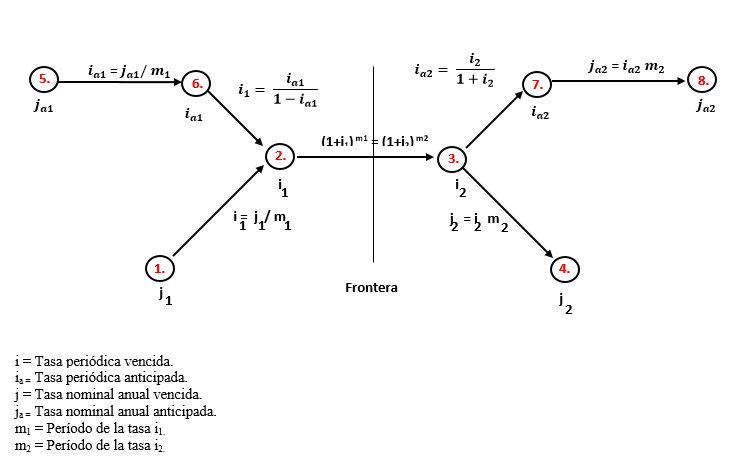
\includegraphics[height = 9.0 cm]{general}\\
	\end{center}
	
	\item b. Declaración de variables:\\
	
	${j_1}$ = 36 \% namv \\	
	${i_1}$ = $\frac{36\% namv}{12 pmv} = 3\% $ pmv\\
	
	$m_{1} $= 12 pmv \\
	${j_2}$ = ? \% nasv\\
	$m_{2} $= 2 psv\\
	
	
	\item c. Declaración de fórmulas:\\
	
	$(1+i)^{m_1} = (1+i)^{m_2}$ \hspace{35 pt} \textit{Equivalencia de tasas}\\
	$j_{1} = i m$\hspace{35 pt} \textit{Tasa nominal anual }\\
	
	\item d. Desarrollo matemático:\\
	Reemplazando\\
	$(1+0,03)^{12} = (1+i_2)^{2}$\\
	$i_{2}$ = 19,405229653\% psv\\
	$j_{2} = i_{2} x m_{2}$\\
	$j_{2} = 19,405229653$\%nasv x 2 psv\\
    $j_{2} = 38,81$\%nasv\\
	\item e. Respuesta\\
	
	$j_{2}$ = 38,81\%nasv\\
\end{itemize}

La solución del problema anterior implicó partir del punto 1 y llegar al punto 4, pasando por los puntos intermedios 2 y 3 De acuerdo con la siguiente gráfica:

\begin{center}
		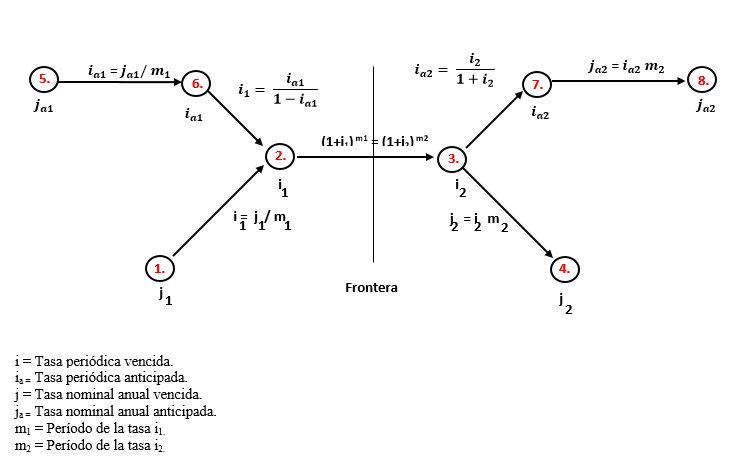
\includegraphics[height = 9.0 cm]{general}\\
\end{center}

En el punto 1 $j_{1}$ = 36\% nasv, en el punto 2 $i_{1} = 3\%$ pmv, en el punto 3 $i_{2} = 19,052$\% psv y en el punto 4 $j_{2} = 38,81\%$ nasv.\\

\textbf{Ejemplo 10}\\

Dado el i=2,5\% periódica mes vencido, hallar una tasa nominal anual trimestral vencida equivalente.\\

\begin{itemize}
	\item a. Diagrama de equivalencia de tasas:\\
	
	\begin{center}
	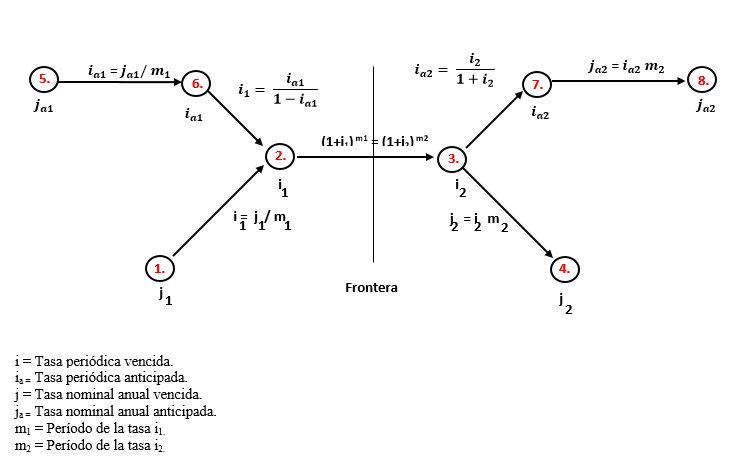
\includegraphics[height = 9.0 cm]{general}\\		
	\end{center}
	
	\item b. Declaración de variables:\\
	
	De la gráfica, se trata de pasar por los puntos 2, 3 y 4.\\
	
	$i_{1}$ = 2,5\% pmv\\
	$m_{1}$ = 12 pmv\\
	$i_{2}$ = ?\% ptv\\
	$m_{2}$ = 4 ptv\\
	
	
	\item c. Declaración de fórmulas:\\
	
	$(1+i)^{m_1} = (1+i)^{m_2}$ \hspace{35 pt} \textit{Equivalencia de tasas}\\
	$j_{2} = i_{2}$  m$_{2}$\hspace{35 pt} \textit{tasa nominal anual}\\
	
	\item d. Desarrollo matemático:\\
	$(1+0,025)^{12} = (1+i_{2})^{4}$\\
	$(1,025)^{\frac{12}{4}}-1 = i_{2}$ \\
	i$_{2}$ = 7,6890625\% ptv\\
	\\
	j$_{2}$ = 7,6890625\% ptv x 4 ptv \\
	
	\item e. Respuesta:\\
	
	j$_{2}$ = 30.756\% natv\\
\end{itemize}

\section{Tasa de interés nominal anual (j) y tasa efectiva anual (EA)}

Según la Superintendencia Financiera de Colombia, SuperFinanciera, la tasa de interés nominal anual es la tasa que el emisor paga al inversionista por un título valor. Las tasas nominales anuales corresponden a la anualización de una tasa periódica, que puede ser diaria, mensual, trimestral, semestral, anual o cualquier otro que se establezca. De igual forma, pueden tener modalidad vencida o anticipada para la liquidación de intereses.\\

\textbf{Tasa de interés efectiva anual:} La tasa de interés efectiva anual, es el instrumento apropiado para medir y comparar, el rendimiento de distintas alternativas de inversión según la Superintendencia Financiera. Según el profesor Javier Serrano, en el libro “Matemáticas financieras y evaluación de proyectos”, la tasa de interés efectiva anual corresponde a aquella tasa de interés que paga de una sola vez al final del año, permite acumular la misma cantidad de dinero que una tasa nominal pagado por período vencido cuando los intereses se reinvierte.\\

Para calcular la tasa efectiva anual, se parte de la fórmula de equivalencia de tasas en donde el periodo es anual vencido.\\ 

	$(1+i)^{m_1} = (1+i)^{m_2}$,
en donde i$_{1}$ = tasa periódica, que anualizada (j$_{1}$) es equivalente a la tasa efectiva anual, para un m$_{1}$ = 1 pav.\\ \\ \\


\textbf{Ejemplo 11}

¿Cuál es la tasa efectiva anual de una tasa del 36\% nominal anual mes vencido?\\

\begin{itemize}
    \item a. Diagrama de equivalencia de tasas:\\
	
	\begin{center}
	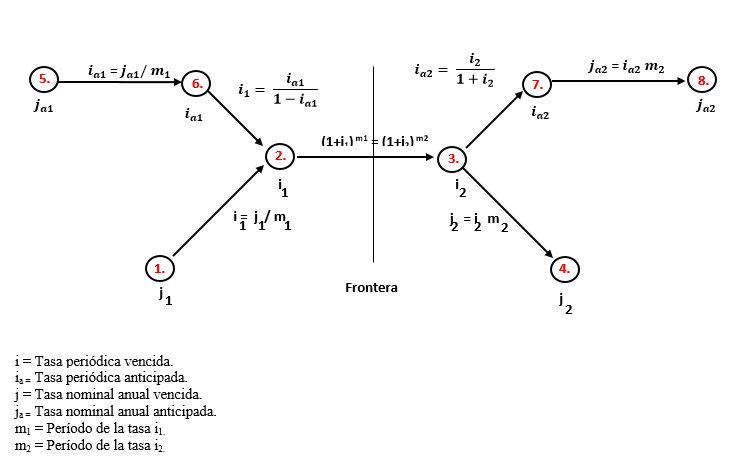
\includegraphics[height = 9.0 cm]{general}\\		
	\end{center}
	
	\item b. Declaración de variables:\\
	$j_{1}$ = 36\% namv \\ 
	m$_{1}$= 12 pmv \\
	$j_{2}$ = ?\% EA\\
	m$_{2}$= 1 pav \\
	\item c. Declaración de fórmulas:\\
		$(1+i)^{m_1} = (1+i)^{m_2}$  \hspace{35 pt} \textit{Equivalencia de tasas}\\
     j= i  m    \hspace{70 pt}\textit{Tasa nominal anual vencida}   \\
	
	\item d. Desarrollo matemático:\\
	
	i$_{2}$ = $\frac{36\%namv}{12 pmv }= 3\% pmv $\\ \\
	
		$(1+i)^{1} = (1+0,03)^{12}$ \\

i$_{2}$ = 42,675 \% pav\\
j$_{2} = 42,675 \% pav x 1 pav = 42,675 \% naav  \equiv
   42,675 \% EA$ \\
	
	\item e. Respuesta:\\

    j$_{2} = 42,675 \% pav\equiv
   42,675 \% EA$ \\
	

\end{itemize}


\textbf{Ejemplo 12}\\

¿Cuál es el interés efectivo anual equivalente a un $j=32\%$ nominal anual trimestre vencido?\\

\begin{itemize}
	\item a. Diagrama de equivalencia de tasas:\\
	
	\begin{center}
	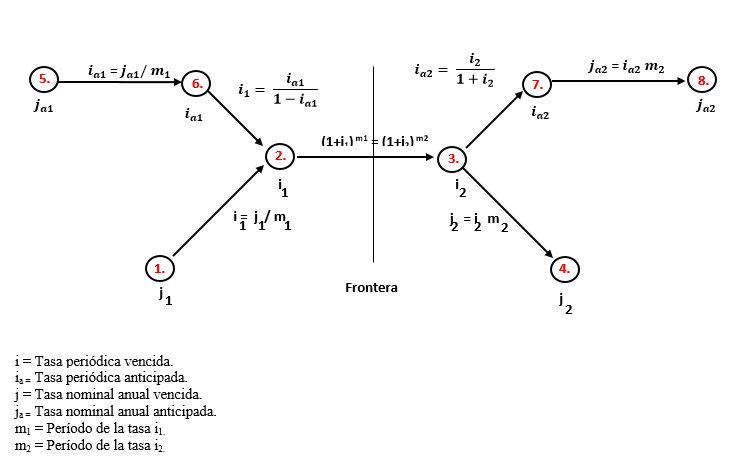
\includegraphics[height = 9.0 cm]{general}\\		
	\end{center}
	
	\item b. Declaración de variables:\\
	
%	Al año se tienen 4 trimestres de forma\\
	$j_{1} = 32$\% natv \Rightarrow $i_{1} = 8$\% ptv\\
	$m_{1}$ = 4 ptv\\	
	$j_{2} = ?\%\ EA$\\ 
	m$_{2}$ =  1 pav\\
	
	
	\item c. Declaración de fórmulas:\\
	$(1+i1)^{m_1} = (1+i2)^{m_2}$ \hspace{35 pt} \textit{Equivalencia de tasas}\\
	j = i m \hspace{35 pt} \textit{Tasa nominal  anual vencida}\\
	
	\item d. Desarrollo matemático\\
	$(1+0,08)^{4} = (1+i_{2})^{1}$\\
	$i_{2}$= 36.05\% pav \Rightarrow $j_{2} = 36$ \% $x 1$ pav $= 36$\% naav \equiv $36$\% EA\\
	
	\item e. Respuesta:\\
	$j_{2} = 36,05$ \% naav  \equiv $36,05$ \% EA\\
	
\end{itemize}

\textbf{Ejemplo 13}\\

¿ Cuál es la tasa efectiva anual equivalente al 36\% nominal anual semestre vencido?\\

\begin{itemize}
    \item a. Diagrama de equivalencia de tasas\\
    
	\item b. Declaración de variables:\\
	$j_{1} = 36$\%nasv \Rightarrow $i_{1} =$\frac{$36$\%nasv}{$2$} $= 18$\% psv \\
	$m_{1} = 2$ psv\\
	
   
    $j_{2}$ = ? \% EA \\
    $m_{2}$ = 1 pav \\
	
	\item c. Declaración de fórmulas:\\
	$(1+i)^{m_1} = (1+i)^{m_2}$ \hspace{35 pt} \textit{Equivalencia de tasas}\\
	j = i m \hspace{35 pt} \textit             {Tasa nominal anual}\\
	
	\item d. Desarrollo matemático:\\
	
		$(1+0,18)^{2} = (1+i_{2})^{1}$ \\
		$i_{2} = 0,39240$  pav\\
		$j_{2} = 39,24$\% $x1$ pav $= 39,24$\% naav \equiv $39,24$\% EA
	
	\item e. Respuesta:\\
	
	$j_{2}$ = 39, 224 \% EA\\
	
\end{itemize}


\textbf{Ejemplo 14}\\

Suponga que una cuenta de ahorros de un banco le paga una tasa efectiva anual del 19\%, ¿Cuál sería la tasa periódica diaria? Asuma un año de 365 días.\\

\begin{itemize}
    \item a. Diagrama de equivalencia de tasas:\\
\begin{center}
	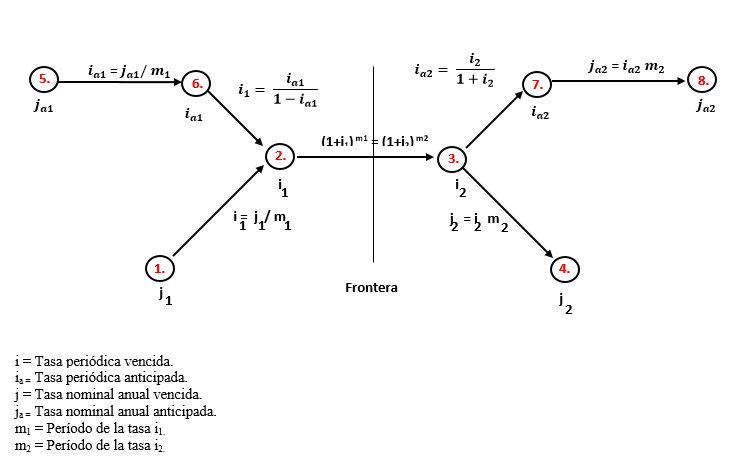
\includegraphics[height = 9.0 cm]{general}\\
\end{center}   
	\item b. Declaración de variables:\\
	
	
	$j_{1} = 19$\% EA \equiv $19$\% naav \Rightarrow $i_{1} = 19$\% pav\\
	m$_{1}$= 1 pav\\
    $i_{2}$ = ? \% pdv \\
    $m_{2}$ = 365 pdv \\
	
	\item c. Declaración de fórmulas:\\
	 $(1+i)^{m1} = (1+i)^{m2}$ \hspace{70 pt}\textit{Equivalencia de tasas:}\\
	j = i m \hspace{15 pt}\textit{Tasa nominal anual}\\
	
	\item d. Desarrollo matemático:\\
	
   
    $(1+0,19)^{1} = (1+i2)^{365}$ \\
	Despejando se obtiene:\\
	
	$i = 1,19 ^{\frac{1}{365}} = 0,00498$ pdv \Rightarrow 0,498\% pdv\\
	
	\item e. Respuesta:\\
	
	i$_{2}$ = 0,498\% pdv\\
	j$_{2}$ = 0,498\% pdv x 365 pdv = 181,77\% nadv\\
	
\end{itemize}



\textbf{Ejemplo 15}\\

¿Cuál es la tasa de interés nominal anual trimestre vencido, equivalente al 18\% nominal anual mes vencido?

\begin{itemize}
    \item a. Diagrama de equivalencia de tasas:\\
\begin{center}
	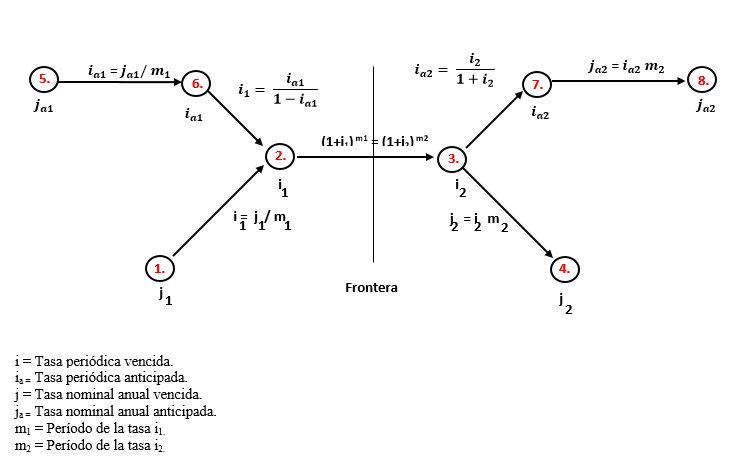
\includegraphics[height = 9.0 cm]{general}\\
\end{center}    
	\item b. Declaración de variables: \\
	$j_{1} = 18$\% namv \Rightarrow $:{i1} =$ \frac{$18$\% namv}{$12$ pmv} $= 1,5$\% pmv\\
	$m_{1}$ = 12 pmv \\
	$j_{2}$ = ? \% natv \\
    $m_{2}$ = 4 ptv \\
   
	

	\item b. Declaración de fórmulas:\\
	
	$(1+i)^{m_1} = (1+i)^{m_2}$\hspace{35 pt}\textit{Equivalencia de tasas}\\
	j = i m \hspace{90 pt}\textit{Tasa nominal anual}\\
	
	\item c. Desarrollo matemático:\\
	
	Primero se calcula el interés mes vencido equivalente a un interés nominal mes vencido del 18\% namv:\\
	
	i$_{1}$= 18\% namv / 12 = 1,5\% pmv
	$(1+0.015)^{12} = (1+i_{2})^{4}$ \\
	
	Despejando:\\
	
	$i_{2} = (1,015)^{\frac{12}{4}} - 1 = 0,04567$ ptv\\
	
	Por lo tanto el interés nominal anual que, pagadero trimestre vencido, es equivalente a un interés del 18\% nominal anual pagadero mes vencido, sería igual a:\\
	
	j = 4 * $i_{2} = 4 * 0,0456 = 0,18271 = 18,271$\% natv\\
	
	Por ello, un interés nominal anual del 18,271\% natv, es equivalente a un interés del 18\% namv.\\
	
	$j_{tv} $=  $18,271$\% natv \equiv 18\% namv\\
	
	\item e. Respuesta:\\
	
	j= 18,271\% natv\\
	
\end{itemize}

\section{Relación entre una tasa de interés anticipada(i$_{a}$) y una tasa vencida(i)}

Para $n = 1$, se tiene 
$i = \frac{I}{P}$ \\
Si \\
$I = F  d$ \\
y \\
$P = F (1 -d)$, \hspace{35 pt}\textit{Tasa nominal anual}\\
remplazando en i \\
$i = \frac {F d} {F (1-d)}$,\hspace{35 pt}\textit{Tasa nominal anual.}\\
factorizando F, tenemos: \\
$i = \frac{d}{(1 - d)}$ \hspace{35 pt}\textit{Tasa nominal anual.}\\
Remplazando $d = i_{a} $,tenemos: \\
$i = \frac{ia}{(1 - ia)}$, \hspace{35 pt}\textit{Tasa nominal anual.}\\
despejando $i_{a}$: \\
$i_{a} = \frac{i}{(1+i)}$ \\

$i = \frac{I}{P} = \frac{F d}{F(1-d)}$\\

$i = \frac{d}{1-d}$\\

Reemplazando d = $i_{a}$\\

Despejando $i_{a}$ = ?\\

$i_{a} = \frac{i}{1+i}$  Tasa periódica anticipada\\

Tasa nominal anual anticipada\\

$j_{a} = i_{a}  m$\\


\section{Gráfica de equivalencia de tasas}

Los puntos que se han colocado del 1 al 8 solo sirven de identificación y no es más que una ampliación de la gráfica mostrada en el ejemplo 9.\\

\begin{center}
	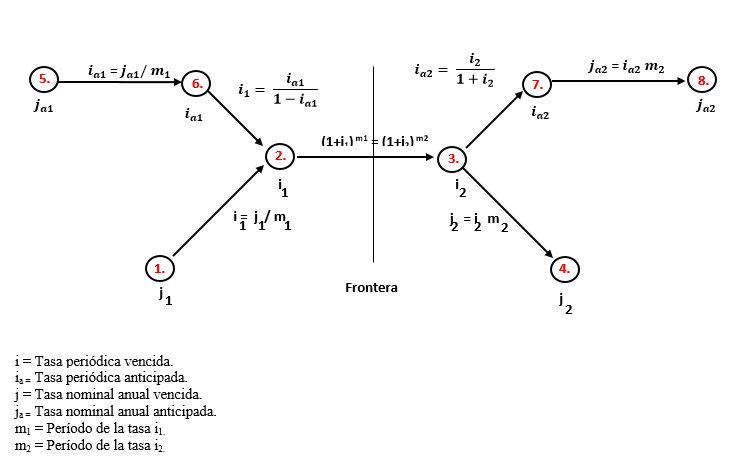
\includegraphics[height = 9.0 cm]{general}\\
\end{center}


\textbf{Observación:} La gráfica equivalencia de tasas, siempre se debe comenzar de un punto de la izquierda y seguir la trayectoria hasta llegar a otro punto situado en la parte derecha.\\

\textbf{Ejemplo 16}\\

Dado el 36\% nominal anual mes vencido hallar:\\

a. Una tasa efectiva anual. \\ 
b. Una tasa nominal anual semestre vencido. \\
c. Una tasa periódica bimensual vencida. \\
d. Una tasa nominal periódica semestre anticipado. \\

a. Diagrama de equivalencia de tasas:\\
\begin{center}
	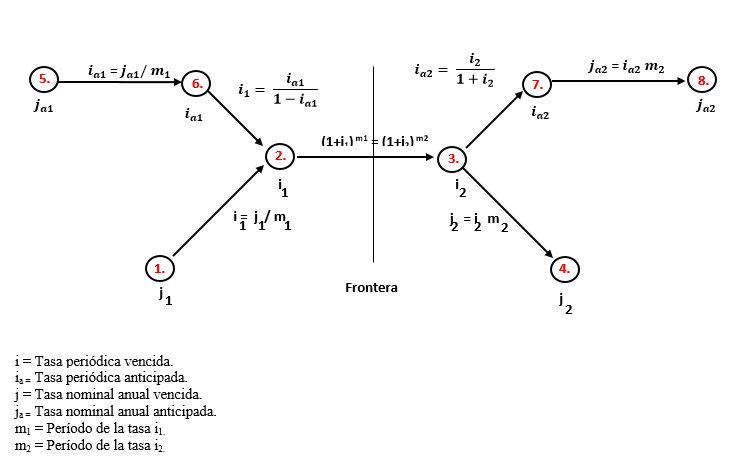
\includegraphics[height = 9.0 cm]{general}\\
\end{center}

\textbf{Solución}\\

\textbf{Parte a.}\\
En el punto (1). j = 36\%namv\\
En el punto (2) $i=\frac{j}{m} = \frac{36\%namv}{12 pmv} = 3$\% pmv\\
Para el paso (2) a (3) planteamos la ecuación $(1+0,03)^{12}= (1+i_{2})^1$ obsérvese que el primer paréntesis se eleva a la potencia 12 porque la tasa del 3\% tiene periodicidad mensual y en un año hay 12 períodos; el segundo paréntesis se eleva a la potencia 1 por que la tasa debe tener una periodicidad anual, es decir es una tasa periodica año vencido; al despejar $i_{2}$ de esta ecuación se tiene:\\

$i_{2}$ = 42,576088685\%  \\j = 42,576\%x1 pav\\
$j = 42,576$\%naav $$\equiv  42,576$$\% EA\\

\textbf{Parte b}.\\
El punto de partida es el punto (1) y el punto de llegada debe ser el punto (4).\\
En el punto (1)  j=36\%namv\\
En el punto (2)  $i=\frac{j}{m} = \frac{36\% namv}{12 pmv} = 3\%$ pmv\\
Para el paso (2) a (3) planteamos la ecuación $(1+i_{1})^{m_{1}}= (1+i_{2})^{m_{2}}$\\
Remplazando $m_{1}$ = 12 pmv y m$_{2}$ = 2 pmv\\

$(1 + 0,03)^{12} = (1 + i2)^2$\\

Obsérvese que el segundo paréntesis se elevó a la potencia 2 por que la tasa debe tener una periodicidad semestral y en un año hay 2 semestres: Al despejar $i_{2}$ de esta ecuación se obtendrá: $i_{2}$ = 19,405229653\% psv.\\


Para el paso de (3) a (4) simplemente multiplicamos el resultado anterior por 2 porque en el lado derecho de la frontera los períodos son semestres y así tenemos:\\ 

j = 19,405229653\%psv\\ x 2 = 38.81\%psv\\
j = 38,81\% nasv\\

\textbf{Parte c}.\\

El punto de partida es el punto (1) y el punto de llegada es el punto 3 del diagrama de conversión de tasas.\\

En los puntos 1 y 2 se tienen los mismos resultados de la parte a o de la parte b por consiguiente en punto 2 i=3\% pmv\\

En el punto 2 al 3 implica el planteo de la ecuación:\\

$(1+i_{1})^{m_{1}} =(1+i_{2})^{m_{2}}$\\
$(1 + 0,03)^{12} = (1 + i)^6$\\

Obsérvese que el exponente del segundo paréntesis debe ser 6 por que en la parte derecha de la frontera los períodos son bimestres y en un año hay 6 bimestres. Al despejar se obtiene:\\ 
i=6,09\% pbv\\

j = 6,09 x 6 = 36,54 nabv\\

\textbf{Parte d.}\\

El punto inicial es el 1- y el punto de llegada debe ser el punto (8).\\ 
En los puntos 1 y 2 los resultados son los mismos que los mostrados en las partes a b o c.\\
El punto 2 al 3 implica planteamiento de la ecuación\\ 

$(1+i_{1})^{m_{1}} =(1+i_{2})^{m_{2}}$\\
$(1+0,03)^{12} = (1+ i2)^2$\\

Y al despejar se tiene que: i2 = 19,405229653 \% psv \\ 
El paso del 3 al 7 implica plantear la ecuación:\\ 

$i_{a} = \frac{i}{1+i}$ \hspace{35 pt} \textit{Tasa periódica anticipada}\\

$\frac{0,19405229653}{1+0,19405229653}$ = 16,2515743317\% psa\\

El paso (7) al (8) implica multiplicar el resultado anterior por 2 y se tiene:\\

$j_{a} = 16,2515743317 x 2 = 32,5\% nasa$\\

Resumen:\\

% \usepackage{multirow}
\begin{table}[]
\centering
\caption{My caption}
\label{my-label}
\begin{tabular}{|c|c|c|c|c|}
\hline
\multicolumn{4}{|c|}{\textbf{\begin{tabular}[c]{@{}c@{}}Equivalencia de tasas nominales anuales (j) con \\ periodicidad y modalidad diferente\end{tabular}}} & \textbf{\%EA}                                                                                 \\ \hline
                                           & Valor                              & Período                        & \textbf{Modalidad}                        & \multirow{6}{*}{\begin{tabular}[c]{@{}c@{}}j = 42,576\% naav\\ \\ = 42,576\% EA\end{tabular}} \\ \cline{1-4}
\multirow{2}{*}{d}                         & 32,5\% na                          & s                              & a                                         &                                                                                               \\ \cline{2-4}
                                           & 36,0\% na                          & m                              & v                                         &                                                                                               \\ \cline{1-4}
c                                          & 36,54\% na                         & b                              & v                                         &                                                                                               \\ \cline{1-4}
b                                          & 38,81\% na                         & s                              & v                                         &                                                                                               \\ \cline{1-4}
a                                          & 42,576\% na                        & a                              & v                                         &                                                                                               \\ \hline
\end{tabular}
\end{table}

\textbf{Ejemplo 17}\\

¿Cuál es la tasa periodica mes anticipada equivalente a una tasa 30\% nominal anual trimestre anticipada?\\

a. Diagrama de equivalencia de tasas:\\

\begin{center}
		\includegraphics[height = 9.0cm]{general}\\
\end{center}

\textbf{Solución:}

Nos situamos en el punto 5 como punto de partida que corresponde a una tasa anual trimestre anticipado y nuestro destino final será el punto 7 que corresponde a una tasa periódica mensual anticipada.\\

En el punto 5 $ j_{a} =30\%$ nata\\
En el punto 6 $i = \frac{i_{a}}{1-i_{a}} = \frac{0,075}{1-0,075}$ = 8,108108\% ptv\\

El paso de 2 a 3 implica el planteo de la ecuación.\\


$(1+i_{1})^{m_{1}} =(1+i_{2})^{m_{2}}$ \hspace{35 pt} \textit{Equivalencia de tasas}\\
$(1+0,08108108)^4 = (1 + i2)^{12}$\\

Obsérvese que en el primer paréntesis quedo elevado a la potencia 4 por que la tasa es periódica trimestre vencido y el segundo paréntesis quedó elevado a la potencia 12 porque los nuevos períodos deben ser mes vencido así:\\

i2 = 2,632779103\% pmv\\

El paso 3 al 7 implica el planteo de la ecuación\\ 


$i_{a} = \frac{i}{1-i}$ \hspace{35 pt} \textit{tasa periódica anticipada}\\

i$_{a}$ = $\frac{0,0263277910}{1+0,0263277910}$ = 2,565\% pma\\

$j_{a} $= 30\% nama\\

\textbf{Ejemplo 18}\\

¿Cuál es la tasa efectiva anual equivalente a una tasa 28\% nominal (258 días) vencido? Asuma el año de 365 días.\\

a. Diagrama de equivalencia de tasas:

\begin{center}
	\includegraphics[height = 9.0 cm]{general}\\
\end{center}

\textbf{Solución:}\\

Iniciamos en el punto 1 y vamos al punto 3.\\
En el punto 1 j = n(258)dv\\

Para llegar al punto 2 sabemos que i = $\frac{j}{m}$ como el período tiene 258 días, entonces en un año habrá $\frac{365}{258}$ = 1.414729 períodos vencidos y al reemplazar en la formula anterior tenemos:\\

$i=\frac{0,28}{1.414729} = 0.197918 = 19.7918\%$ p258dv\\

i = 19.7918\% p258dv


Para el paso de 2. a 3.\\

$(1 + i_{1})^{m_{1}} = (1+ i_{2})^{m_{2}}$ \hspace{35 pt}\textit{Equivalencia de tasas}\\
$(1 + 0.197918)^{\frac{365}{258}} = (1 + i)^1$ \\
Despejando se tiene que i=29,10797\% pav\\
j=im\\
=29,10797\%x1 pav\\
$j=29,10797\%naav \equiv 29,10797$\% EA\\

\textbf{Ejemplo 19}\\

¿Cuál es la tasa nominal anual (150 días) vencido equivalente a una tasa del 20\% nominal anual (200 días) anticipada? Asumir el año de 365 días.\\

\textbf{Solución}\\

a. Diagrama de equivalencia de tasas:

\begin{center}
	\includegraphics[height = 9.0 cm]{general}\\
\end{center}

Una tasa con período 200 días anticipada es representada con $i_{a}$.\\

Por lo tanto salimos del punto 5 y vamos al punto 4.\\

En el punto 6 $i_{a}$ = 20\% período  (200 días) anticipada.\\

En el punto 2- $i = \frac{i_{a}}{1-i_{a}} = \frac{0,2}{1-0,2} $= 0,25 p(200 días) a\\

Para ir del punto 2 al punto 3 debemos tener en cuenta que si un período tiene 200 días entonces en 1 año habrá $\frac{365}{200}$ períodos, de igual forma, si un período tiene 150 días en un año habrá $\frac{365}{150}$ períodos por tanto podemos plantear la siguiente ecuación:\\

$m_{1}= \frac{365dias}{200dias}$\\

$m_{2} = \frac{365dias}{150dias}$\\

$(1 + 0.25)^{\frac{365}{200)}} = (1 + i2)^{\frac{365}{150}}$\\


Para despejar la i es necesario deshacer el paréntesis de la derecha y para ello es necesario que quede elevado a la potencia 1, por tanto habrá que multiplicar los exponentes de la ecuación anterior por $\frac{150}{365}$, entonces la ecuación queda así:\\ 

$(1 + 0,25)^{\frac{365}{200}\frac{150}{365}} = (1+i)^{\frac{365}{150}\frac{150}{365}}$\\

$(1 + 0,25)^{\frac{150}{200}} = (1 + i)^1 $\\

1.1821770 = 1 + i\\

Despejando se tiene i=18.2177\% período 150 días que corresponde al punto 3.
Para llegar al punto 4 se aplica la formula j = i m\\

Entonces $j = 18.2177 x \frac{365}{150} = 44.33 \%na 150$dv\\

$j = 20\%\ (200dias)\ a\ \equiv 44.33\%na\ 150dv$

\section{Ecuaciones de valor}

Es muy frecuente cambiar una o varias obligaciones por otra u otras nuevas obligaciones. La solución de este problema es elemental y para solucionarlo es necesario usar ecuación de valor, que es una igualdad de valores ubicados en una sola fecha denominada fecha focal.\\

La fecha focal se representa gráficamente por una línea a trazos y por las letras ff y es la fecha en que debe hacerse la igualdad entre ingresos y egresos. La ubicación de la fecha focal no altera la respuesta final, por tal motivo la ubicación de la fecha focal se deja a libre elección de la persona que va a resolver el problema. (En interés simple, la posición de la fecha focal sí causa variación en la respuesta final y por esta razón normalmente es el acreedor quien decide donde ubicarla).\\

El principio fundamental de una ecuación de valor, que viene a ser el mismo principio fundamental de las finanzas, establece que la sumatoria de los ingresos debe ser igual a la sumatoria de los egresos ubicados ambos en la fecha focal, esto es:

\begin{center}
	$\sum ingresos = \sum egresos(en la ff)$\\
\end{center}
Naturalmente que el traslado a la fecha focal de cada una de las cantidades debe hacerse usando la fórmula del valor futuro o la fórmula del valor presente, segun el caso, utilizando una tasa de interés llamada el rendimiento normal del dinero que es la tasa que en promedio cobra el sistema financiero.\\

El enunciado de una ecuación de valor también puede ser expresado así:

\begin{center}
	$\sum deudas = \sum pagos(en la ff)$\\
\end{center}

Mirando un balance el principio puede ser expresado así:\\

\begin{center}
	$\sum activos = \sum pasivos + capital(en la ff)$\\
\end{center}

Como en cualquier proyecto los ingresos se representan por flechas hacia arriba y los egresos se representan por flechas hacia abajo entonces, mirando la gráfica de flujo de caja podemos expresar el principio fundamental de una ecuación de valor de esta otra forma:\\

\begin{center}
	$\sum de\ lo\ que\ esta\ para\ arriba = \sum de\ lo\ que\ esta\ para\ abajo(en\ la\ ff)$\\
\end{center}

La sumatoria de los ingresos en pesos de hoy menos la sumatoria de los egresos en pesos de hoy recibe el nombre de valor presente neto o valor actual neto (en la calculadora se representa por VAN y en EXCEL se representa por VNA).\\

La tasa a la cual la sumatoria de los ingresos es igual a la sumatoria de los egresos se denomina tasa interna de retorno que en el texto se representará por TIR.\\

En capitulo posterior analizaremos más en detalle los conceptos de VPN: valor presente neto y TIR, estos conceptos son de suma importancia en la evaluacion de proyectos.\\

\textbf{Ejemplo 20}\\

Una persona se comprometió a pagar \$250.000 en 3 meses, \$300.000 en 8 meses y \$130.000 en 15 meses. Ante la dificultad de cumplir con las obligaciones tal como están pactadas solicita una nueva forma de pago así: \$60.000 hoy, \$500.000 en 12 meses y el saldo en 18 meses. Suponiendo que el rendimiento normal de la moneda es del 36\% nominal anual mes vencido, determinar el valor del saldo.\\

\begin{itemize}
	\item a. Diagrama de flujo de caja.\\
	\begin{center}
		\includegraphics[height = 6.0 cm]{2_17_1}\\
	\end{center}
	
	\begin{center}
		\includegraphics[height =6 cm]{2_17_2}\\
	\end{center}
	
	\item b. Declaración de variables:\\
	
	
	$j = 36\%namv$
	\\$ i = \frac{36\%}{12}$pmv = 3\% pmv
	\\
	$P_{1} = \$250.000; \hspace{35 pt}$n_{1} = +5 pmv;\\
	P_{2} = \$300.000;$\hspace{37 pt}n_{2} = 0 $ pmv\\
	P_{3} = \$130.000$; \hspace{30 pt} 	$n_{3} = -7 pmv;\\
	$P_{4} = \$60.000; \hspace{40 pt}n_{4} = +8 $ pmv;\\
	P_{5} = \$500.000$; \hspace{32 pt}	$n_{5} = -4 pmv;\\ \\ P$_{6}$=\$?\\ 
	n_{6} = -10 $ pmv;\\
	   Fecha focal (ff): en el mes 8.\\    
  	
	
	\item c. Declaración de fórmulas:\\
	
	$F = P(1+i)^n$ \hspace{35 pt} \textit{Valor futuro dado un valor presente}\\
	$P = F(1 +i)^{-n}$\hspace{33 pt} \textit{Valor presente dado un valor futuro}\\
	
	\item d. Procedimiento matemático\\
	
	$F_{1} + F_{2} + P_{3} = F_{4} + P_{5} + P_{6}$ \hspace{35 pt}\textit{Ecuacion de valor.}\\
	
	La ecuación de valor puede ser escrita, en la fecha focal ff 8 para el período octavo, así:\\
	
	$\$250.000(1+0,03)^5 + \$300.000(1+0,03)^0 + \$130.000(1+0,03)^{-7} = \$60.000(1+0,03)^8 + \$500.000(1+0,03)^{-4} + P_{6}(1+0,03)^{-10}$\hspace{33 pt} \textit{Ecuación de valor}\\
	
	Al despejar 	$P_{6}$ de esta ecuación se tiene:
	
	$P_{6} = \$235.549.16$\\
	
	\item e. Respuesta:\\
	
	La solución será: $P_{6}$ = \$235,549.16\\
	
	
\end{itemize}

\textbf{Ejemplo 21}\\

Una deuda de \$15.000 fue contraída hace 2 meses con fecha de vencimiento en 4 meses, esta posee un interés del 24\% nominal anual trimestre vencido y otra deuda de \$25.000 contraída hace un mes con vencimiento de 8 meses e intereses del 28\% nominal anual semestre vencido, se van a cancelar mediante dos pagos de igual valor, efectuados el primero el día de hoy y el segundo en 6 meses. Con un interés del 30\% nominal anual mes vencido y el segundo en 6 meses, con un interés del 30\% nominal anual mes vencido, determinar el valor de los pagos.\\

\begin{itemize}
	\item a. Diagrama de flujo de caja:
	\begin{center}
		\includegraphics[height = 6.0 cm]{2_18_1}\\
	\end{center}
	
	\begin{center}
		\includegraphics[height = 7.0 cm]{2_18_2}\\
	\end{center}
	
		\begin{center}
		\includegraphics[height = 7.0 cm]{2_18_3}\\
	\end{center}
	
	\item b. Declaración de variables:\\
	
	Deuda 1:\\
	$j_{1}$ = 24\% natv\\	
	$i_{1}$ = 6\% ptv\\	
	$n_{1}$ = 2 ptv\\
	
	$P_{1}$ = \$15.000    \\
    $F_{1}$ = \$?
	
	Deuda 2\hspace{5 pt}:\\
	
	$j_{2}$ = 28\% nasv\\	
	$i_{2}$ = 14 \% psv\\	
	$n_{2}$ = 1,5 psv 
	
	$P_{2}$ = \$25.000   \\ 
    $F_{2}$ = \$? \\
	
	Deuda equivalente:\\
	
	$j_{3}$ = 30\% namv\\	
	$i_{3}$  = 2.5\% pmv\\
	
	$ff$ = fecha focal: mes 6\\
    
    $P_{3} = F1$\\    
    $F_{3} = F2$\\
    
	
	\item c. Declaración de fórmulas:\\
	
	$F = P(1+i)^n$\hspace{35 pt} \textit{Valor futuro dado un valor presente}\\
	$P = F(1+i)^{-n}$\hspace{35 pt} \textit{Valor presente dado un valor futuro}\\
	
	\item d. Procedimiento matemático:\\
	
	Primero debemos liquidar el valor de cada deuda en la fecha de su vencimiento\\
	
	$F_{1} = \$15.000(1 + 0,06)^2 = \$16.854$\\
	$F_{2} = \$25.000(1 + 0,14)^{1.5} = \$30.429,67$\\
	
	A continuación el planteamiento de la ecuación de valor será:\\ 
	
	\$ 16.854(1 +0,025)^2 + \$30.429,67(1 + 0,025)^{-2} = X(1 + 0,025)^6 + X$ \hspace{35}\textit{Ecuación de valor}\\
	
	\item e. Respuesta:\\
	
	La solución será: X = \$21.609,84\\
	
	
\end{itemize}

\textbf{Ejemplo 22}\\

Una persona debe pagar \$10.000 con vencimiento en 3 meses, \$15.000 a 10 meses y \$20.000 con vencimiento en un año. Si hace un pago único de \$45.000, hallar la fecha en que debe hacerse, suponga una tasa del 18\% nominal anual mes vencido.\\
Si consideramos la fecha focal (ff) en el mes 12:\\

\begin{itemize}
	\item a. Diagrama de flujo de caja:\\
	\begin{center}
		\includegraphics[height = 6.0 cm]{2_19_1}\\
	\end{center}
	
	\begin{center}
		\includegraphics[height = 5.5 cm]{2_19_2}\\
	\end{center}
	
	\item b. Declaración de variables:\\
	$j$ = 18\% namv\\ i = 1,5\%pmv\\
	
	$P_{1} = \$10.000; \hspace{35 pt}$n_{1}$ = +9pmv ;\\ P_{2} = \$15.000; \hspace{35 pt}$n_{2} = 2$ pmv\\
	
 $P_{3} = \$20.000$ \hspace{35 pt}	$n_{3}$ = 0 pmv \\  $P_{4} = \$45.000$ \hspace{35 pt} $n_{4}$ =12-n$\\
	
	
	
	\item c. Declaración de fórmulas:\\
	
	$F = P(1+i)^n$ \hspace{35 pt} \textit{Valor futuro }\\
	$P = F(1+i)^{-n}$ \hspace{35 pt} \textit{Valor presente}\\
	
	\item d. Procedimiento matemático:\\
	
	El planteamiento de la ecuación de valor será:\\
	
	$\$10.000(1+0,15)^9 + \$15.000(1 + 0.015)^2 + \$20.000(1 + 0,015)^0 = \$45.000(1+0.015)^{12-n}$ \hspace{35 pt} \textit{Ecuacion de valor}\\ 
	
	$\$46.887,27 = \$45.000(1,015)^{12-n}$\\
	
	$\frac{\$46.887,27}{\$45.000} = (1,015)^{12-n}$\\
	
	$1,00419394 = (1,015)^{12-n}$\\
	
	$log1,00419394= (12-n)log1,015$\\
	
	$(12 - n) = \frac{log1,00419394}{log1,015}$\\
	
	$(12 - n) = 2,759409869$\\
	
	$n = 9,240959 pm$\\
	
	\item e. Respuesta:\\
	
	El pago único de \$45.000 lo debe hacer a los 9,240959 meses.\\
	
	En la respuesta anterior existen 9 meses + 0,24059 de mes, y mediante una proporción se puede establecer el número de días que hay en la fracción de mes así:\\
	Un mes tiene 30 días, en 0,24059 de mes, ¿Cuántos días hay?\\
	
\begin{table}[]
\centering
\label{my-label}
\begin{tabular}{|c|c|}
\hline
\textbf{MES} & \textbf{DÍAS} \\ \hline
1            & 30            \\ \hline
0,24         & x             \\ \hline
\end{tabular}
\end{table}

	Despejando se tiene que X = 7,2177 días.\\
	
	La fecha exacta sería 9 meses con 7,2177 días.\\
	
\end{itemize}

\textbf{Ejemplo 23}\\

Una persona debe pagar \$70.000 en 3 meses y \$85.000 en 8 meses; ante la imposibilidad de cancelar las deudas en las fechas previstas le ofrece al acreedor que le cancelara \$50.000 en 4 meses y \$130.000 en 12 meses. Si el acreedor acepta esta nueva forma de pago ¿Qué tasa de interés periódica mes vencido estará pagando?\\

\begin{itemize}
	\item a. Diagrama de flujo de caja:\\
	
	\begin{center}
		\includegraphics[height = 6.0 cm]{2_21_1}\\
	\end{center}
	
	\begin{center}
		\includegraphics[height = 6.0 cm]{2_21_2}\\
	\end{center}
	
	\item b.Declaración de variables:\\
	
	i=?\% pmv\\
	$F_{1} = \$70.000$ ; \hspace{25}$n1 = -3$ pmv\\
    $F_{2} = \$ 85.000$; \hspace{25}$n2 = -8$pmv \\
    $F_{3} = \$ 50.000$; \hspace{25}$n3 = -4$ pmv\\
    $F_{4} = \$130.000$; \hspace{22}$n4= -12$pmv \\
	
	\item c. Declaración de fórmulas:\\
	
	$F = P(1 + i)^n$ \hspace{35}\textit{Valor futuro}\\
	$P = F(1 + i)^{-n}$\hspace{35}\textit{Valor presente}\\
	$P_{1} + P_{2} = P_{3} + P_{4}$\hspace{35}\textit{Ecuación de valor}\\
	
	\item d. Procedimiento matemático:\\
	
	La incógnita es la tasa i, en consecuencia el planteo de la ecuación de valor será:\\ \\
	$\$70.000(1+i)^{-3}+\$85.000(1+i)^{-8} = \$50.000(1+i)^{-4} + \$130.000(1+i)^{-12}$
	
	El procedimiento para resolver este problema de forma manual es el siguiente:\\
	
	\begin{itemize}
		\item Se iguala toda la ecuación a cero, y se simplifica por mil:\\
		
		$70(1 + i)^{-3} + 85(1 + i)^{-8} - 50(1 + i)^{-4} - 130(1 + i)^{-12} = 0$\\
		
		\item  Para resolver esta ecuación utilizaremos el método de ensayo y error combinado con una interpolación, el método consiste en escoger una tasa $i_{1}$ y calcular el valor que toma la función $f_{1}$, luego haremos lo mismo con una tasa $i_{2}$ y calculamos el valor que toma la función $f_{2}$, lo importante es que el valor de las funciones $f_{1} y f_{2}$ sean de signo diferente, si al hacer los ensayos las funciones salen del mismo signo, habrá que hacer nuevos ensayos hasta que obtengamos las funciones con signo diferente.\\
		
		\item 	De acuerdo a lo anterior hacemos un primer ensayo con $i_{1}$ = 2\% pmv , entonces al remplazar en la ecuación esta ya no va a ser igual a 0 y su resultado será:\\
		
		$70(1 + 0,02)^{-3} + 85(1 + 0,02)^{-8} - 50(1 + 0,02)^{-4} - 130(1 + 0,02)^{-12} = -10,18714$\\
		
		\item 	Ahora procederemos con el ensayo de $i_{2} =3\% pmv$ y la ecuación con su resultado será:\\
		
		$70(1 + 0,03)^{-3} + 85(1 + 0,03)^{-8} - 50(1 + 0,03)^{-4} - 130(1 + 0,03)^{-12} = -4,44404$\\
		
		\item Como el valor de la función en ambos casos es negativo entonces tenemos que hacer un nuevo intento con otra tasa de interés hasta que cambie de signo, por eso ensayamos con $i_{3} = 4\%$ pmv y la ecuación será:\\
		
		$70(1 + 0,04)^{-3} + 85(1 + 0,04)^{-8} - 50(1 + 0,04)^{-4} - 130(1 + 0,04)^{-12} = -0,40058$\\
		
		\item Tomamos los resultados correspondientes al 3\% y a 4\% por ser los más cercanos y los que presentan diferente signo y los colocaremos de la siguiente forma:\\
		
		\begin{center}
			\includegraphics[height = 3.0 cm]{2_22}\\
		\end{center}
		
		\item Ahora planteamos una proporción, teniendo en cuenta las diferencias mostradas en los corchetes y siempre manteniendo el mismo orden, por ejemplo: la diferencia pequeña es a la diferencia grande del lado izquierdo igual que la diferencia pequeña es a la diferencia grande del lado de la derecha.\\
		
		\begin{center}
			$\frac{3-i}{3-4} = \frac{-4.44404 - 0}{-4.44404 - 0.40058}$\\
		\end{center}
		
		
		
	\end{itemize}
	
	\item e. Respuesta:\\
	
	Al despejar i de la ecuación anterior tenemos: i= 3,91735 pmv.\\
	
\end{itemize}

\textbf{Observación:} La interpolación produce un error que es despreciable siempre y cuando el intervalo que se toma para interpolar no sea muy grande, en la práctica financiera un punto porcentual es el máximo permitido para que el error sea despreciable, en este caso hemos usado un punto porcentual porque hemos interpolado entre el 3\% y el 4\%. La respuesta exacta con 7 decimales es: 3.9104765\% pmv.



\cleardoublepage
\phantomsection
\setlength{\columnsep}{0.75cm}
\printindex


%----------------------------------------------------------------------------------------




\part{Capítulo tres}
\graphicspath{ {img/ch3/}, {img/} }

%----------------------------------------------------------------------------------------
%	CHAPTER 3
%----------------------------------------------------------------------------------------

\chapterimage{ima2} % Chapter heading image


\chapter{Aplicaciones de interés compuesto}
\section{Fórmulas del capítulo}
\begin{spacing}{1.5}
\begin{center}
\begin{tabular}{ |p{6cm}|p{7cm}| p{2cm}|}
\hline 
\rowcolor{orange!50}
\begin{center}\textbf{Fórmula} \end{center} & \begin{center} \textbf{Nombre}\end{center} & \begin{center} \textbf{Excel} \end{center} \\ \hline                       

$i =i_{1} + i_{2} + (i_{1})(  i_{2})$ & Equivalencia de tasas de referencia & - \\ \hline 

$ i_{R} = \frac{i-i_{f}}{1+i_{f}} $ &   Tasa de interés real & - \\ \hline

 
\end{tabular}
\end{center}
\end{spacing}


Muchas son las aplicaciones que tiene la fórmula de interés compuesto, aquí solo daremos algunas, las que consideramos están más de acuerdo con el plan del texto. Para empezar examinaremos los depósitos a término fijo y certificados de depósito a término.\\



\section{Depósito a término fijo}


La misión de un intermediario financiero consiste en conseguir dinero prestado generalmente del público y volverlo a prestar a otras personas, pero a una tasa más alta. Para conseguir el dinero del público debe ofrecer una tasa de interés e incentivar a los inversionistas a que le traigan sus ahorros, a esta tasa se le denomina tasa de captación. Cuando va a prestar estos dineros lo hace a una tasa mayor denominada tasa de colocación.\\

\subsection{Certificado de depósito a término}
Es el certificado que se recibe por depósitos de sumas de dinero. Los plazos pueden ser de 30 días en adelante siendo los más comunes los de 30, 60, 90, 180 y 360 días. Pueden emitirlos los bancos comerciales, corporaciones financieras y compañías de financiamiento comercial. La tasa de interés por su depósito está determinada por el monto, el plazo y las condiciones existentes en el mercado al momento de su constitución. Son nominativos y no se pueden redimir antes de su vencimiento.\\ 



\textbf{Ejemplo 1}\\

Supongamos que una persona invierte \$600.000 en un depósito a término fijo en 6 meses, si le garantizan una tasa del 24\% nominal anual mes vencido, determinar la tasa efectiva anual y el valor del documento suponiendo una retención en la fuente sobre utilidades del 7\% sobre las utilidades.\\

\begin{itemize}
	\item a. Diagrama de flujo :\\
	
	%%imagen 1
	
	\begin{center}
		\includegraphics[height=5.0cm]{3_1}
	\end{center}
	
	\item b. Declaración de variables :\\
	F=\$?\\
	VP = \$600.000 \\	
	j a encontrar=? \%EA\\
	j dada= 24\% namv \\	
	n = 6 pmv \\
	RF= 7\% I
	
	\item c. Declaración de formulas :\\ 
	$VF=P(1+i)^n$ \hspace{35}\textit{Valor futuro dado un valor presente}\\
	j = im \hspace{35} \textit{        Tasa nominal anual}\\
	$(1+i_{1})^{m_{1}} = (1+i_{2})^{m_{2}}$\hspace{35} \textit{Equivalencia de tasas}\\
	$RF = 7\%\ I$     \textit{        Retención en la fuente} \\ 
    $I = F - P$      \textit{Monto del interés}\\ 
    $F\ neto = F - R$     \textit{         Valor futuro neto}\\
	
	\item d. Desarrollo matemático:\\
    Despejando:\\
    De la formula de equivalencia de tasas\\
    $ (1+0,02)^{12} = (1+i)^{1} $\\
    $i = (1 + 0,02)^{12} -1 = 0,26824179$\\
    $j = 0,26824179 x1 = 0,26824179 EA$\\
    $j = 26,824179\% EA$\\
    $i = 26,48\%$ pav\\
    $j = 26,48\% x1= 26,48\%\ naav = 26,48\%\ EA$\\
	VF= \$$600.000(1+0,02)^6$\\
	VF= \$675.697,45\\
	I = F - VP = \$675.697,45 - \$600.000\\
	I = F - VP = \$75.697,45\\
	RF = 0,07 x \$75.697,45 = \$5.298,82\\
	F$_{final}$ = \$675.697 - \$5.299 = \$670.398\\
	
	\item e. Respuesta:\\
	El valor del documento después de impuestos es de \$675.697,45 que es menor que F = \$675.697,45 y obviamente se reduce la tasa de nominal anual mes vencido j = 24,84\% naav .\\
	
	Observación
	\begin{itemize}
		\item La rentabilidad después de impuestos se puede calcular así:\\ \$670.398 = \$$600.000(1+i)^6$
		\item De donde se obtiene\\
		$i$ = 1,866232288 \% pmv\\
		$j$ = 1,866232288 \% x 12 = 22,3947874\% namv \\
		$(1 + i_1)^{m_1} = (1 + i_2)^{m_2}$\\
        para la EA, $m_2$\ = 1 y luego \\
        $j = i m$\\
        $j = 24,84\%\ EA,\ inferior\ al\ 26,82\%\ EA$\\
		\item Por equivalencia de tasas: 
		$i$ = 24,84\% EA (después de impuestos)\\
	\end{itemize}
	
\end{itemize}
De lo visto hasta el momento podemos concluir que si el depósito a término fijo gana el 26,84\% EA antes de impuestos, después de impuestos se reduce al 24,84\% EA, sin embargo esto no es más que una utopía porque el inversionista entregó al principio \$600.000 los cuales tenían un cierto poder adquisitivo y cuando le devuelven el dinero su poder de compra se ha disminuido por efectos de la inflación y se pregunta cuál sería la rentabilidad del depósito a término después de impuestos e inflación en términos de EA? (pendiente a retornar más adelante).\\

\subsection{Inflación (i_f)}
Mide el crecimiento del nivel general de precios de la economía. La inflación es calculada mensualmente por el DANE sobre los precios de una canasta básica de bienes y servicios de consumo para familias de ingresos medios y bajos. Con base en éstas calcula un índice denominado Índice de Precios al Consumidor (IPC). La inflación corresponde a la variación periódica de ese índice.\\
\\
Hacemos énfasis en que la inflación y la deflación son fenómenos internos a un país. (La devaluación si es un fenómeno económico externo a un país).\\


\subsection{Índice}
Es un indicador que tiene por objeto medir las variaciones de un fenómeno económico o de otro orden referido a un valor que se toma como base en un momento dado. Relación de precios, de cantidades, de valores entre dos períodos dados.

\subsection{Índice de precios al consumidor (IPC)}
Variación que entre un mes y otro presentan los precios de bienes y servicios de consumo final correspondientes a una canasta típica, donde se incluyen los servicios educativos, de salud, de alimentos y combustible, entre otros.

\subsection{Tasa promedio de captaciones Básica de Superfinanciera (TBS)}
Es la tasa promedio de captación a través de CDT y CDAT de las entidades financieras, calculada diariamente por la Superintendencia Financiera para diferentes plazos.	

\section{Devaluación (idev)}	
La pérdida de valor de una moneda frente a otra moneda se denomina devaluación, por ejemplo, habrá devaluación si inicialmente hay que pagar \$1500 por un dólar y un año más tarde hay que pagar \$2000 por el mismo dólar. En este caso la devaluación del año es igual a la variación de precio sobre el precio inicial, esto es: \\

devaluación = $\frac{\$2000-\$1500}{\$1500} = 0,333333 $ = 33,33\% pav \\

Lo contrario de la devaluación se denomina revaluación que significa que habrá que pagar menos pesos por el mismo dólar, por ejemplo, si al principio del año hay que pagar \$1500 por un dólar y al final del año hay que pagar \$1200 entonces la revaluación será variación de precio sobre el precio inicial así: \\

revaluación = $\frac{\$1200-\$1500}{\$1500} = -0,2$ = -20\% pav \\



\subsection{LIBOR (London Interbank Offer Rate)}
Tasa de interés anual vigente para los préstamos interbancarios de primera clase en Londres y Europa.\\ \\



\textbf{Ejemplo 2}\\
Un inversionista residente en Colombia adquiere un documento que vale U\$300, gana un interés del 6\% nominal anual año vencido (naav) en dólares a un plazo de un año. El tipo de cambio actual es US\$ 1 = \$1500 y se estima una devaluación del peso con respecto al dólar durante ese año del 20\% efectivo anual. Calcular la rentabilidad que se podía obtener. ¿Cuál es la rentabilidad neta, una vez descontada la retención en la fuente del 7\%?

\begin{itemize}
	\item a. Diagrama de flujo de caja:
	
	%imagen 2
	\begin{center}
		\includegraphics[height=5.0cm]{3_2}
	\end{center}
	
	
	\item b. Declaración de variables en dólares:\\
	j= 6\% naav en US$\\
    n=1 pav\\
    Dólar: 1US$=$1500\\
    j dev= 20\% EA
	
	
	\item c. Declaración de fórmulas\\        
		
		$ F = {P(1+i)^{n} $\hspace{35}\textit{ Valor futuro}\\     
	
	\item d. Desarrollo matemático:\\
	Las condiciones iniciales son: US\$300 y en pesos $300 x 1500 = \$450.000$\\
	\\ %imagen3
	
	
	
	Las condiciones finales en dólares son:\\
	$F = P(1+i)^n $\hspace{35}\textit{ Valor futuro dado un valor presente}\\
	$F = US\$300(1 + 0,06)^1 = US\$318$\\\\
	Para calcular las condiciones finales en pesos primero debemos calcular el tipo de cambio que regirá dentro de un año. \\
	
	Declaración de variables en pesos:\\
	Como la devaluación es del 20\% EA, dentro de un año un dólar valdrá\\ $VF = \$1.500(1+0,2)^ {1} = \$1.800$ y los US\$318 valdrán US\$ $318\textbf{x}\frac{\$1.800}{US\$1} = \$572.400$ tal como se aprecia en la gráfica.\\

		US$\$318 \textbf{x}\frac{\$1.800}{US\$1} = \$572.400 $ \hspace{35}\textit{ Ecuación de valor}\\

	%imagen 4
	\begin{center}
		\includegraphics[height=4.0cm]{3_4}
	\end{center}
	
	
\end{itemize}
Como el inversionista reside en Colombia la rentabilidad que él necesita conocer se obtiene aplicando la fórmula del interés compuesto a los valores iniciales y finales en pesos (si el inversionista fuera residente en E.E.U.U la rentabilidad se obtendrá entre valores iniciales y finales, pero en dólares).  \\

\begin{itemize}
	\item a. Diagrama de flujo de caja:\\
	%imagen 5
	\begin{center}
		\includegraphics[height=5.0cm]{3_5}
	\end{center}
	
	\item b. Declaración de variables en pesos:\\
	Pc= \$450.000\\ F = \$572.400\\ 
	j=?\% naav\\
	n = 1 pav\\
	\item c. Declaración de fórmulas:\\
	$F = P(1+i)^n$\hspace{35} \textit{Valor futuro}\\
	\item d. Desarrollo matemático:\\
	$\$572.400 = \$450.000(1+i)^1$\hspace{35} \textit{Ecuación de valor}\\
	$i=27,2\% pav,\ \rightarrow \ j = 27,2 x1 = 27,2 \%\ EA$ \\
	$I = \$572.400 - \$450.000 = \$122.400$ \\
    $RF = 0,07 x \$122.400= \$8.568$ \\
    $F neto = \$572.400 - \$8.568 = \$563.832$ \\\\
    Aplicando la fórmula del valor futuro: \\
    $\$563.832 = \$450.000(1+i)^1$ , despejando $i = ?$ \\
    $i = 0,25296$naav \equiv  $j = 25,296\% EA$ \\
	\item e. Resultado:\\
    
    La rentabilidad que se podía obtener es 27,2\%\ EA. y la rentabilidad neta, una vez descontada la retención en la fuente del 7\%\ es 25,296 \%\ EA\\

\end{itemize}

\section{Tasas combinadas o tasas equivalentes de referencia}
En el caso anterior el inversionista ganará dos tasas, una tasa la de interés en dólares 6\% (naav) y otra la tasa de devaluación 20\% EA equivalente a 20\% (naav) (porque al final del año va a recibir más pesos por el mismo dólar).\\

Cuando se combina una tasa $i_{1}$ con una tasa $i_{2}$, con el objetivo de facilitar los cálculos se puede utilizar la tasa combinada i. Para este fin se usa la siguiente fórmula.\\
\centerline{$ i = i_{1} +i_{2} + (i_{1})( i_{2})$ \hspace{15}\textit{ Tasas combinadas}\\}
\textbf{Nota} Se utiliza únicamente para el cálculo de tasas de interés anuales\\




\textbf{Ejemplo 3}\\
Resolver el ejemplo 2 usando la tasa combinada\\

\textbf{Solución:}\\

\begin{itemize}
	\item a.Diagrama de flujo:\\
	
	%imagen 6
	\begin{center}
		\includegraphics[height=3.5cm]{3_6}
	\end{center}
	
	
	\item b.Declaración de variables:\\
	$j_{1} = 6\%\ naav$\\
	$j_{2} = 20\%\  naav$\\
	\item c. Declaración de fórmulas:\\
	$i =i_{1} + i_{2} + i_{1}  i_{2}$\hspace{35}\textit{ Tasas combinadas}\\
	$j =i  m$\hspace{35}\textit{ Tasa nominal anual}\\
	\item d.Desarrollo matemático:\\
	$i_{1}= \frac{6 \%\ naav}{1} = 6\% $pav \\
	$i_{2}= \frac{20 \%\ naav}{1} = 20\% $pav \\
	$i= 0,06 + 0,2 + 0,06 x 0,2 = 0,272 = 27,2\% pav,\\ j = 27,2\% x1 = 27,2\ \%\ naav$ \hspace{35}\textit{ Ecuación de valor}\\
	\item e.Respuesta:\\
	Usando la tasa combinada obtenemos que el resultado es 27,2\% EA\\
	
\end{itemize}


\section{Tasa deflactada o tasa real}
Al hacer el análisis sobre proyectos de inversión es necesario tener en cuenta que la inflación afecta la rentabilidad real del proyecto y que siempre se desea obtener una rentabilidad superior a la inflación. Para calcular la rentabilidad real podemos hacer uso de la fórmula asumiendo que la inflación $i_{f} = i_ {1} $, que la rentabilidad $i_{R} = i_ {2} $ y que la rentabilidad que en total paga es i, por tanto se tiene:\\
\begin{align*}
	i= i_{f} + i_{R} + i_{f} i_{R}
\end{align*}

Despejando $i_{R}$ se tiene 
\begin{align*}
	i_{R} = \frac{i-i_{f}}{1+i_{f}}\hspace{35}\textit{ Tasa de interés real}
\end{align*}



\textbf{Ejemplo 4:}\\
Calcular la rentabilidad que gana el inversionista del ejemplo 2 teniendo en cuenta que la inflación para el año en el que se hizo la inversión fue del 18\% efectivo anual. ¿Cuál es la rentabilidad neta una vez descontada la Retención en la fuente y la inflación? \\\\

\textbf{Solución:}\\

\begin{itemize}
	\item a. Diagrama de flujo:\\
		%imagen 6
	\begin{center}
		\includegraphics[height=5cm]{3_4_1}
	\end{center}
	\item b. Declaración de variables:\\
    
    $i=27,2\% pav $\\
	$i_{f} = 18\%$  EA \equiv 18\%naav \\
    $i_{f} = \frac{j}{m} = \frac{18\%}{1} = 18\%$ pav \\
    $i_{RF} = 25,296\% pav$\\ 
	\item c. Declaración de fórmulas:\\
	$ i_{R} = \frac{i-i_{f}}{1+i_{f}} $\hspace{35}\textit{ Tasa de interés real}\\
	\item d. Desarrollo matemático:\\
	
	$i_{R} = \frac{0,272-0,18}{1+0,18} = 0,077966 = 7,8\% $pav\\
	$i^{*}_{R} = \frac{(0,25296-0,18)}{(1 + 0,18)}$ \hspace{35}\textit{ Tasa de interés luego de retencion en la fuente}\\
    $i^{*}_{R} = 6,18305085\%$ pav \\
    $j^{*}_{R} = 6,18305085\%$ EA \\
	\item e. Respuesta.\\
	La rentabilidad sin descontar la retención en la fuente  fue del 7,8\% pav.\\
	\end {itemize}
	
	
	Retomando el ejemplo 3 podemos concluir que si el depósito a término fijo gana el 26,84\% EA antes de impuestos, después de impuestos se reduce al 24,84\% EA, sin embargo esto no es más que una utopía porque el inversionista entregó al principio \$600.000 los cuales tenían un cierto poder adquisitivo y cuando le devuelven el dinero su poder de compra se ha disminuido por efectos de la inflación ($i_{f}= 18\% $pav$ $) y se pregunta cuál sería la rentabilidad del depósito a término después de impuestos e inflación en términos de 7,8\%pav y una vez descontada la retención en la fuente queda en 6,18\%.\\
	
	
	\section{Combinación de tasas}
	Hay muchos créditos atados a una tasa principal, por ejemplo a la inflación más unos puntos adicionales, estos puntos adicionales se denomina el spread, suponiendo que la inflación fuera del 10\% efectivo anual y que el spread sea de 5 puntos, entonces la tasa a la cual se cancelará el crédito se puede calcular aplicando la fórmula de las tasas combinadas: \\
	
	$i= 0,1 pav + 0,05 pav + 0,1 x 0,05 = 0,155 pav \equiv 15,5\% pav $ \rightarrow  $j = 15,5\% pav x1 pav = 15,5\%naav \equiv 15,5 \%EA$ \\
	
	Cuando la tasa principal viene dada en forma efectivo anual para agregarle el spread se usa la fórmula de combinación de tasas, pero si el spread se le adiciona a una tasa nominal entonces el spread simplemente se suma a la tasa principal, por ejemplo: \\
	
	Si un préstamo para vivienda se otorga a la tasa de los depósitos a término fijo-DTF (tasa principal) más 8 puntos y suponiendo que la tasa de depósito a término fijo -DTF lo mismo que la sea del 17\% nominal anual trimestre anticipado, entonces la tasa del crédito será: \\
	
	$i = i_{1} + i_{2}
i = 17\%nata + 8\%nata = 25\% nata$\\\\ Las tasas equivalente nominales se suma en igual periodo y modalidad, en tasas efectivas anuales se aplica la equivalencia de tasas de referencia.\\
	
	Por equivalencia de tasas se concluye que es equivalente al 29,45\% efectivo anual.\\
	
	\textbf{Observación:} Para créditos es costumbre que la tasa de depósito a término fijo -DTF lo mismo que la tasa de captación de las corporaciones-TCC se expresan en nominal anual trimestre anticipado y en tasa de captación de la tasa de depósito a término fijo -DTF y de la tasa de captación de las corporaciones-TCC se expresa en efectivo anual.\\
	
	
	
	\textbf{Ejemplo 5}\\
	
	Supongamos que una persona tiene un préstamo hipotecario al IPC + 4 puntos ¿Cuál debe ser el spread si se cambia a otro plan cuya tasa es la DTF +X? Suponga que el IPC = 8\% efectiva anual y que la DTF = 18,67\% nominal anual trimestre vencido, en donde
IPC: Tasa del Índice de Precios al Consumidor
DTF: Tasa de Depósito a Término Fijo promedio \\
	
	\textbf{Solución:}\
	\\
	
	\begin{itemize}
		\item a. Diagrama de flujo\\
		No se Requiere \\
		\item b. Declaración de variables\\\\
		$j_{1}= 8\% EA \\ j_{2} = 18,67\% nata$\\
		\item c.Declaración de fórmulas:\\\\
		IPC + 4 = DTF + X  Ecuación de valor\\
		ECUACION DE EQUIVALENCIA \\
        
        Tasa del crédito = IPC + 4 puntos efectivos anuales = DTF + X (spread en \% nata) \\
        $i = i_1 + i_2 +i_1 * i_2$ \\
		$i_{a}= \frac{i}{1+i}$\\
		$(1 + i_{1})^{m_{1}} = (1 +i_{2})^{m_{2}}$\\
		$j_{a} = i m$\\
		\item d. Desarrollo matemático:\\\\
		IPC+4 = 0,08 + 0,04 + 0,08 x0,04\\
		Tasa del crédito = IPC + 4 puntos\\
        Tasa de crédito inicial= 0,08 + 0,04 + 0,08x0,04 EA\\
		IPC+4 = 12,32\% pav equivalente a 12,32\% EA \\
		$(1 + 0,1232)^1 = (1 + i) ^4$ Fórmula de equivalencia de tasas para convertir la tasa de crédito del 12,32\% EA a una periódica trimestre vencido y a su vez a la tasa nominal anual trimestre anticipada.\\
		i= 2,947137112\% ptv\\
		
		$i_{a}= \frac{0,02947137112}{1+0,02947137112} = 0,0286275\%$ pta\\
		$j_{a} = 2,86875\% * 4 = 11,451\%$ nata\\
		
		Tasa de crédito equivalente= DTF + 4 (\%nata) \\
        Tasa de crédito equivalente = 11,45 \% nata = 18,67\% nata + X \%nata \\
        Entonces X = 11,451\% nata - 12,32\% nata = -7,219\% nata \\
		DTF + X = 0,1867 + X nata \\
		0,11451 = 0,1867 + X; de donde X = -0,07219 \\
		X = -7,219\% nata\\
		
		\item e. Respuesta\\
		
		Finalmente podemos concluir que si se cambia de plan tendrá que ser la DTF menos 	7,219\%	nata\\
		
	\end{itemize}
	
	\textbf{Observación 1:}En Colombia el spread se da en puntos que son adicionales a la tasa principal, en Europa y Estados Unidos el spread se acostumbra a dar en puntos básicos. Un punto básico es igual al 0,01\% de forma que 400 puntos básicos corresponden a un spread de 4 puntos.\\
	
	\textbf{Observación 2:}A pesar de que la Libor es una tasa efectiva, es costumbre que el spread simplemente se sume a la Libor sin hacer uso de la tasa combinada, La razón es que éstas tasas son muy pequeñas y la diferencia de resultados entre un método y otro es prácticamente nula.\\
	
	\textbf{Ejemplo 8}\\
	Una industria tiene actualmente contratado un préstamo con una corporación financiera a la tasa del TCC+3 puntos. ¿Cuál debe ser el spread en puntos básicos de forma tal que financieramente sea indiferente el préstamo en la corporación financiera o en el mercado de Londres? Suponga los siguientes índices: \\
	
	TCC = 15,3 \% nata \\
    $i_{dev}$ = 22\% EA. Interés devaluación del peso Colombiano con respecto a la libra esterlina. \\
    Libor = 5,2\% EA. Tasa de interés del mercado europeo \\
	
	Solución:
	\begin{itemize}
		\item a. Diagrama de flujo:\\
		No se requiere
		\item b. Declaración de variables:\\
		
		TCC = 15,3\% nata\\
		$i_{dev} = 22\%$ EA\\
		Libor = 5,2\% EA\\
		\item c. Declaración de formulas:\\
		
		$i_{dev} + Libor + X = TCC + 3$  Ecuación de valor\\
		\item d. Desarrollo matemático:\\
		
		TCC + 3 puntos= 15,3\%nata + 3\%nata = 18,3\%nata\\
		j crédito = TCC + 3 puntos nata = 15,3\% nata + 3\% nata = 18,3\% nata, tasas nominales sumas los dígitos. En tasas efectiva anual aplicamos la formula de las tasas combinadas: $i = i_{1} + i_{2} + i_{1} i_{2}$ \hspace{35}\textit{  Equivalencia de tasas de referencia} \\
        
        $j_{c} = 18,3\% nata$ \\
        $j_{c} = ?$ EA en Londres \\
		
		18,3\%npta ~ 20,601\% EA . A partir de las del crédito en TCC, 18,3\% nata, calculamos la tasa Anual Efectiva equivalente, encontrando la tasa periódica ($j = i*m$)
        y a partir de la tasa periódica anticipada llegamos a la tasa periódica vencida ($i_{a} = \frac{i}{(1+i)}$).\\
        Teniendo la tasa periódica vencida utilizamos la formula de las tasas equivalentes:
        $(1 + i_{1})^{m_{1}} = (1 + i_{2})^{m_{2}}$, en donde $m_{1}$ es igual 1, periodo anual vencido de liquidación de la tasa EA.\\
		$i_{dev} + Libor + X = 22\% + (5,2+ X)\%$\\
		crédito equivalente = 22\% EA + (libor + X) \%\ EA = ? \% EA, por la fórmula de combinación de tasas, por ser tasas EA.\\
		0,28344 + 0,0122 + X = 0,20601. (Despejar la X) \\
		X = -6,35\% \\
		\item e. Respuesta:\\
		
		Lo que significa que cobrar TCC + 3 puntos es lo mismos que cobrar devaluación más Libor menos 6,35 puntos\\
	\end{itemize}
	
	
	\section{Aceptaciones bancarias y financieras}
	\textbf{Ver link} https://prezi.com/ewsfyuf6vepz/aceptaciones-bancarias/\\
	
	Las aceptaciones bancarias y financieras son letras de cambio con cargo a un comprador de bienes manufacturados que una entidad financiera avala o garantiza su pago al poseedor de la aceptación de vencimiento. El plazo máximo es de un año. Cuando la entidad financiera que da el aval es un banco se denomina aceptación bancaria, si es otro tipo de entidad financiera se denomina aceptación financiera.\\
	
	Las aceptaciones en general son títulos que se expiden a la orden del proveedor, no son divisibles, no son gravables en el mercado primario.\\
	
	\textbf{Ejemplo 9}\\
	Supongamos que un proveedor de bicicletas (puede ser la fábrica) recibe un pedido de compra de 50 unidades para un almacén por valor de \$ 5 millones, pero el almacén pide un plazo de 90 días para pagar. El proveedor acepta el pedido, pero solicita que una entidad financiera garantice el pago futuro, por tal motivo el dueño del almacén se dirige a su banco y le solicita que expida una aceptación bancaria por \$ 5 millones con vencimiento en 90 días, el banco le entrega al almacén la aceptación y éste se la entrega al proveedor, este último puede guardar la aceptación y cobrarla al banco a su vencimiento o puede negociarla en el mercado secundario.\\
	
	%imagen ejemplo 9
	\begin{center}
		\includegraphics[height=4.0cm]{3_7}
	\end{center}	
	
	Puede ocurrir que el fabricante se encuentre en un país distinto al del almacén y si el banco no tiene sucursal en ese otro país deberá tener corresponsales (es decir bancos que lo representen en ese otro país). Si el proveedor necesita el dinero antes del vencimiento, puede ofrecer en venta la aceptación y para ello tiene dos opciones: Venderla al mercado extra bursátil, que tiene la ventaja de no pagar comisiones a intermediarios porque se negocia en forma directa o venderla al mercado bursátil, es decir en una bolsa de valores, a través de un intermediario de bolsa conocido como corredor de bolsa que cobra una comisión por sus servicios de intermediación.\\
	
	Es obvio que, al vencimiento de la aceptación, el dueño del almacén deberá cancelar al banco el valor de ésta e independientemente de si el almacén le paga o no al banco la aceptación, el banco sí tendrá que pagar en la fecha de vencimiento el valor nominal de la aceptación al tenedor de ésta. A continuación, presentamos una gráfica más completa donde se muestra la trayectoria de la aceptación bancaria.\\
	
	%imagen ejemplo 9_2
	\begin{center}
		\includegraphics[height=5.0cm]{3_8}
	\end{center}	
	
	\textbf{Primera opción}: Supongamos que faltando 40 días para el vencimiento, el proveedor debido a un estado de iliquidez, decide vender la aceptación en el mercado extra bursátil, (el inversionista que adquiere esta aceptación puede ser un particular, una compañía de financiamiento comercial, una leasing, etc.) Supongamos que la tasa convenida es del 30\% periódico año vencido es diferente a una tasa de descuento del 30\% del valor final = d. Tomar el año de 365 días.\\
	Es costumbre calcular el Pc como un porcentaje del valor que tendrá la aceptación al vencimiento. (El valor al vencimiento se denomina valor de maduración o valor de redención y lo representaremos por F).
	Haciendo el cálculo por cada \$ 100 de valor de maduración se tendrá: \\\\\\\\\\\\\\
	
	\begin{itemize}
		\item a.Diagrama de flujo\\
		\begin{center}
			\includegraphics[height=5.0cm]{3_9}
		\end{center}	
		\item b. Declaración de variables\\
		
		P = \$? \\
		VF = \$100\\
		i=30\% pav\\
		$n = \frac{40}{365}$ pav	       
		\item c. Declaración de formulas:\\
		
		F =  $P(1+i)^n$ \hspace{35}\textit{Valor futuro}\\
		\item d. Desarrollo matemático:\\
		
		VP = $\$100(1+0,3)^\frac{-40}{365}$ = \$97,1657\\
		Pc=\$5.000 x 97,1657\% = \$4.858,285\hspace{35}\textit{Ecuación de valor}\\
		Entonces si el precio de compra Pc es de \$97,1657 el precio de compra para una aceptación de 100 pesos el precio de compra para \$5000 es 5000x (0,971657).\\
		
		\item e. Respuesta\\
		El valor que se invirtió fue \$4.858,285\\
	\end{itemize}
	
	\textbf{Segunda opción:} El proveedor decide descontar la aceptación en el mercado bursátil y en tal caso debe recurrir a un corredor de bolsa (quienes son los únicos autorizados para negociar en la bolsa) y supongamos que el corredor le dice que en la bolsa este tipo de operaciones se está registrando al 30\% periódica 40 días vencido, esta tasa se denomina tasa de registro porque es la tasa que queda registrada en las computadoras de la Bolsa y la representamos por $i_{R}$. Con base en la tasa de registro se puede calcular el precio de registro así: \\
	$P_{v}= \$100  (1 + 0,35)^{\frac{-40}{365}}$ Equivalente al 97.1657 \$.\\
	El precio de este registro en pesos será: 97,1657\$ x \$5'000.000 = \$4.858.285\\
	De esta forma en las computadoras de la Bolsa va a aparecer en venta esta aceptación por valor de 97.1657\% de su valor nominal de registro y que a ese precio produce una rentabilidad del 30\% periódica 40 días vencidos.\\
	Pero además el corredor le dice que para que la aceptación sea inscrita en bolsa tendrá que pagar una comisión que representaremos como COMv (Comisión de venta).\\
	Supongamos que la comisión de venta sea del 0,5\% en rentabilidad entonces la tasa total de descuento será: \\
	$i_{R} + COMv = 30\% + 0,5\% = 30,5\%$ p(40d)v\\
	Esta nueva tasa se denomina tasa de cesión o tasa del vendedor.\\
	Con base en la tasa de cesión podemos calcular el valor de cesión o sea el valor que recibe el vendedor para la aceptación. El precio de cesión lo representaremos por Pv (precio de venta), \\
	$P_{v}  = \$100(1+0,35)^\frac{-40}{365} = \$97,1248 $ equivalente a 97.1248\%\\
	$P_{v} = 97.1248 < P_{R} = 97.165$\ porque está cediendo un valor al comisionista vendedor.\\
	El precio de venta en pesos o precio de cesión en pesos será: 5.000.000 \text{x} 0,971248 = \$4.856,240\\
	
	\textbf{Observación:} El valor de la comisión de venta se puede hallar por la diferencia entre los precios de venta y el precio de registro esto es: \\
	COMv= 4.858.285 - 4.856.240 = \$2.405\\
	
	\textbf{Ejemplo 10}\\
	
	Supongamos que un inversionista desea adquirir la aceptación bancaria del ejemplo anterior la cual figura con una tasa de registro del 30\% periódico 40 días vencido y con precio de registro P_{R} = 97,165\% pero él también sabe que para adquirirla deberá pagar una comisión a un corredor de bolsa lo cual hará variar el precio que él debe pagar y también la rentabilidad que él pueda obtener.\\
	
	Supongamos que la comisión que cobra un corredor por la compra es del 0,475\% periodo 40 días periodo vencido\\
	¿Cuál es el precio del inversionista? $P_{c} = \$$?, que incluye la comisión de bolsa de comprador, el precio de registro y la comisión del comisionista vendedor. El punto de referencia es el precio de registro P_{R}.\\
	¿Cuál es la rentabilidad del inversionista? $i_{c} =? \%$ periódica 40 días vencido, o $j =? nadv$\\
	
	\textbf{Solución}\\
	\begin{itemize}
		\item a. Diagrama de flujo\\
		\begin{center}
			\includegraphics[height=8.0cm]{3_10}
		\end{center}	
		\item b. Declaración de variables\\ 
		$i_{c} = 30\% - 0,475\% = 29,525\% p(40dv)\\
		VPc = ?\\
		$n= -\frac{40}{365}\\$\\
		P_{R}=?$\\
		\item c.Declaración de formulas\\
		P = $F(1+i)^{-n}$ \hspace{35}\textit{Valor presente}\\
		\item d. Desarrollo matemático:\\
		Pc = $ \$100(1+0,29525)^\frac{-40}{365} = \$97.2047$ \hspace{35}\textit{Ecuación de valor} \\
		$P_{R}$ = \$97.2047\% x \$5.000.000 = \$4.860,245\\
		Pc-$P_{R}$ = \$4.860,235 - \$4.858,285 = \$1.950\\ 
		\item e. Respuesta\\
		Precio del Inversionista = \$ 97.2047 y la rentabilidad inversionista fue de 29,52\% P= 40 dv \\

		
	\end{itemize}
	\textbf{Observación:} En el mercado bursátil el precio del vendedor es diferente al precio del comprador debido a la comisión de los corredores de bolsa, pero en el mercado extrabursátil estos valores son iguales dado que no hay comisión.\\
	
	En el ejemplo anterior hemos mostrado el procedimiento de negociación en los mercados extra bursátil y bursátil, pero por simplicidad no hemos incluido el impuesto y la comisión que cobra el banco por la expedición de la aceptación bancaria. En el siguiente ejemplo incluiremos este factor.\\
	
	\textbf{Ejemplo 11}\\
	El dueño del almacén solicita al banco una aceptación bancaria por \$5 millones, que entregará al proveedor (fabricante) para que le entreguen la mercancía; para que el banco preste este servicio le cobra al dueño del almacén una comisión que puede ser del 1\% por mes pagadero en forma anticipada sobre el valor de la aceptación, esto es 1\% x 5.000.000 = \$50.000 por cada mes y por los 3 meses que dura la aceptación será: \$50.000 x 3 = \$150.000, además habrá que pagar otra carga impositiva que es el IVA, que en el momento es del 16\%, así que en pesos el IVA será: 16\% x \$150.000 = \$24.000 de manera que el costo total de apertura de la aceptación bancaria para el dueño del almacén viene a ser \$150.000 + \$24.000 = \$174.000. El $P_{R}$ = \$4.860,245 del ejemplo anterior.\\
	¿Cuál es el precio de aceptación? \\
	¿Cuál es la rentabilidad? \\
	
	\begin{itemize}
		\item a. Diagrama de flujo\\
		\begin{center}
			\includegraphics[height=4.0cm]{3_11}
		\end{center}	
		\item b.Declaración de variables\\
		rf=7\% de las utilidades\\
		VF = \$5.000.000\\
		$VP_{R}$ = \$4.858,285\\
		\item c. Declaración de formulas\\
		RF = rf * (F - $P_{R}$) \\
		\item d. Desarrollo matemático\\
		
		Si la aceptación es vendida en el mercado bursátil, ya no habrá IVA (puesto que ya fue pagado en el momento de la apertura de la aceptación) pero en cambio habrá otra carga impositiva que grava las utilidades sobre activos financieros denominada retención en la fuente la cual representaremos RF cuya tarifa actual (1999) es del 7\%, de las utilidades, es decir que se aplica a la diferencia entre el valor de redención y el precio del registro.\\
		Si la aceptación es vendida en el mercado bursátil 40 días antes del vencimiento a un inversionista, según el ejemplo 10, el precio de registro es \$4858,258, en consecuencia, la retención en la fuente la podemos calcular así: \\
		\begin{center}
			RF = 0,07(\$5.000.000 - \$4,858,258) = \$ 9,920\\
		\end{center}
		
		\item e. Respuesta:\\
		\begin{center}
			RF = \$9920
		\end{center}
		En consecuencia, el comprador (que viene a ser el inversionista) deberá pagar el precio de compra más la retención en la fuente lo cual viene a dar: \\
		\begin{center}
		    $Pc = \$4.860,235 + \$9.920 = \$4.870,155$
		\end{center}
		
	\end{itemize}
	\textbf{Observación 1:}La nueva $i_{c}$ se reduce al 27,137419\% periódica 40 días vencido con respecto a la $i_{R}$ del 30\% periódica 40 días vencido, e incluye la comisión bursátil y la retención en la fuente (por la totalidad de rendimientos en 90 días).\\
	
	\textbf{Observación 2:} El $i_{v}$ se aumenta X\%EA con respecto al $i_{R}$ del 30\% EA, incluye la comisión bursátil del vendedor, comisión de expedición de la aceptación bancaria e IVA:\\
	\\
	\\
	\\
	\\
	\textbf{Tabla de rentabilidad en anual efectivo}\\
	
	\textbf{Ejercicio 12}\\
	
	Supongamos que faltando 10 días para el vencimiento el inversionista del ejemplo anterior decide venderlo y para esta época se están negociando en Bolsa con una tasa del 28\% período 10 días vencido, por lo tanto la tasa de registro debe ser del 28\% período 10 días Vencido y el precio de registro será: \\
	\begin{itemize}
		\item a.Diagrama de flujo:\\
		
		\item b.Declaración de variables

			Pr = \$?\\ F = \$100\\ i= 28\% p(10d)v \\$n= \frac{10}{365}$p(10d)v\\

		\item d.Declaración de formulas:\
		
			$P=F(1+i    )^{-n}$\hspace{35}\textit{Valor presente}\\
		
		\item e. Desarrollo matemático
	
			$P_{R}=\$100 (1+0,28)^\frac{-10}{365}$ = 99,32595\% \hspace{35}\textit{Ecuación de valor}\\
	
		En pesos el precio de registro será: 99,3595\% x \$5.000.000 = \$4.966,298\\
		Por lo tanto, la retención en la fuente será RF = 0,07*(\$5.000.000 - \$4.966,298) = \$2.359\\
		Suponiendo que las comisiones de compra y venta sean c/u del 0,5\% en rentabilidad la tasa del vendedor viene a ser 28\% + 0,5\% = 28,5\% período 10 días vencido y el precio de venta será:
		\begin{center}
		$	P_{V} = 100(1+0,285)^\frac{-10}{365}$ = 99,3153\% equivalente a 99.3153\% * \$5.000.000 = \$4.965,765\\
		\end{center}
		Por lo tanto el vendedor además de recibir los \$4.965.765 también debe recibir lo correspondiente a la retención en la fuente (\$2,359), En consecuencia el vendedor recibirá:\\
		\begin{center}
		$P_{V}$ = \$4.966.830 + \$2.539 = \$4.969.189
		\end{center}
		Para el comprador se tiene:
		\begin{center}
			Tasa de compra ic = 28\% - 0,5\% = 27,5\% p10dv
		\end{center}
		Precio de compra:
		\begin{center}
			Pc = $100(1+0,275)^\frac{-10}{365}$ = 99,3366\% equivalente a 99,3366\%*\$5.000.000 = \$4.966.830
		\end{center}
		El total que debe pagar el comprador será el precio de compra más la parte de retención en la fuente que la Bolsa le devuelve al vendedor, esto es:
		\begin{center}
		VPc Neto= 	\$4.966.830 + \$2.359 = \$4.969.189
		\end{center}
		\item e. Respuesta\\
		\textbf{Observación 1:} El primer inversionista pagó por retención en la fuente \$9.920 y le reintegraron \$2.359 esto significa que en total pagó: \$9.920-\$2.359	= \$7.561 y el segundo inversionista pagó \$2.359\\
		\textbf{Observación 2:} La constitución de aceptaciones no implica desembolsos de dinero en forma inmediata ni por parte de la entidad financiera ni por parte del comprador, salvo el IVA y la comisión de intermediario financiero, lo demás es una obligación futura.\\
		\textbf{Observación 3:} Si una aceptación no es cobrada al vencimiento, el emisor debe consignar el valor de esta en el Banco Agrario, sin embargo el emisor da un período de gracia antes de hacer la correspondiente consignación.
	\end{itemize}
	\medskip
	
	\textbf{Ejemplo 13}\\
	
	Una aceptación bancaria por \$80 millones con fecha de vencimiento el 17 de diciembre de 1999 es adquirida en 22 de julio de 1999 por un primer inversionista con un descuento de 28\% período 28 días vencidos y es cedida a un segundo inversionista el 14 de octubre de 1999. Si el segundo inversionista desea ganarse el 32\% período días vencido, utilice un interés comercial (año de 360 días) \\
	¿Cuál es la ganancia en pesos del primer inversionista? \\
	¿cuál es la rentabilidad periódica días vencido del primer inversionista? \\
	
	Si tomamos en cuenta que debemos usar un año de 360 días entonces los días que hay entre el 22 de julio y el 17 de diciembre son 145 que se calculan así: \\
	
	\begin{center}
		\includegraphics[height=5.0cm]{3_12}
	\end{center}
	
	Los días que hay entre el 14 de octubre y el 17 de diciembre se calculan así:
	

	\begin{center}
		\includegraphics[height=3.0cm]{3_13}
	\end{center}
	
	\textbf{Solución}\\
	\begin{itemize}
		\item a. Diagrama de flujo\\
		\begin{center}
			\includegraphics[height=4.0cm]{3_14}
		\end{center}
		\item b. Declaración de variables\\
		$i_{1} = 28\% pav$ \\
		$n_{1} = \frac{145}{360}$ pav\\
		$i_{2} = 32 \% pdv$\\
		$n_{2} =\frac{63}{360}$pdv\\ 
		 $n_{3} = 145$ días - 63 días = 82 pdv.\\

			$P_{c2}-P_{c1} = ?$\\\\

		\item c. Declaración de formulas\\
		
			P = $F(1+i)^{-n}$ \hspace{35}\textit{Valor presente}\\
		
		\item d. Desarrollo matemático\\
		$Pc_1 = \$80.000.000(1+0,28)\frac{-145}{360}$ = \$ 72.428.283,64 \simeq \$72.428.284 \hspace{35}\textit{Ecuación de valor}\\
		$Pc_2 = \$80.000.000(1+0,32)\frac{-63}{360}$ = \$ 76.206.067,12\\ 
		\item e. Respuesta:\\
		La ganancia del primer inversionista será:\\
		\begin{center}
			$Pc_2 - Pc_1 = \$76.206.067 - \$72.428.284 = \$3.777.783$\\
		\end{center}
	\end{itemize}
	En este caso el tiempo se puede hallar calculando los días que hay entre el 22 de julio y el 14 de octubre usando el procedimiento anterior, o, también por diferencia de días entre el total que es 145 y los que hay entre la fecha de compra del segundo inversionista y a la fecha de vencimiento que vienen a ser 63 días, entonces esta diferencia viene a ser: 145 - 63 = 82
	\begin{center}
		\$76.206.067 = $\$72.428.284(1+i)\frac{82}{360}$
	\end{center}
	De donde se obtiene que i= 25,01\%\ período 82 días vencidos \\
	La rentabilidad del segundo inversionista obviamente es del 32\% periodo (63 días vencidos).

	
	
	
	
	
	
	
	
	%\chapter{Modelos de Conteo}
	
	%\section{Introducción}\index{Introducción}
	
	
	
	%----------------------------------------------------------------------------------------
	%	PART
	%----------------------------------------------------------------------------------------
	
	%\part{Parte Dos}
	
	%----------------------------------------------------------------------------------------
	%	CHAPTER 3
	%----------------------------------------------------------------------------------------
	
	%\chapterimage{ima2} % Chapter heading image
	
	
	%Anexos
	%\chapter*{Anexos}
	%\addcontentsline{toc}{chapter}{\textcolor{ocre}{Anexos}}
	
	
	
	
	%----------------
	
	%----------------------------------------------------------------------------------------
	%	BIBLIOGRAPHY
	%----------------------------------------------------------------------------------------
	
	%\chapter*{Bibliografía}
	%\addcontentsline{toc}{chapter}{\textcolor{ocre}{Bibliografía}}
	%\section*{Books}
	%\addcontentsline{toc}{section}{Books}
	%\printbibliography[heading=bibempty,type=book]
	
	%\begin{itemize}
	%\item
	
	
	%\end{itemize}
	
	
	%----------------------------------------------------------------------------------------
	%	INDEX
	%----------------------------------------------------------------------------------------
	
	\cleardoublepage
	\phantomsection
	\setlength{\columnsep}{0.75cm}
	\printindex





%----------------------------------------------------------------------------------------
%	PART
%----------------------------------------------------------------------------------------


\part{Capítulo cuatro}

\graphicspath{ {img/ch4/}, {img/} }

%----------------------------------------------------------------------------------------
%	CHAPTER 4
%----------------------------------------------------------------------------------------

\chapterimage{ima2} % Chapter heading image


\chapter{Serie uniforme vencida y anticipada}



\section{{Fórmulas del capítulo}}

\begin{spacing}{1.2}
\begin{center}
\begin{tabular}{ |p{4.2cm}|p{5.7cm}| p{4cm}|}
\hline 
\rowcolor{orange!50}              %
\begin{center}\textbf{Fórmula} \end{center} & \begin{center} \textbf{Nombre}\end{center} & \begin{center} \textbf{Excel} \end{center} \\ \hline                        


$VP = R  \frac{1-(1 + i)^{-n}}{i} $\hspace{35 pt} & Valor presente serie uniforme vencida & VNA(i;R1;R2;R3;...)\\ \hline 


	 $VF = R  \frac{(1 + i)^n-1}{i} $ &  Valor futuro serie uniforme vencida \hspace{35 pt} & VF(i;n;;VA,0)\\  \hline 


$VP_{a} = R  \frac{1-(1 + i)^{-n}}{i}  (1 + i) $ \hspace{35 pt} & Valor presente serie uniforme anticipada   & - \\ \hline 

$VF_{a} = R  \frac{(1 + i)^n-1}{i}   (1 + i) $ \hspace{35 pt} &  Valor futuro serie uniforme anticipada  & VF(i;n;;VA,1) \\ \hline 


 
\end{tabular}
\end{center}
\end{spacing}

\textbf{Ejemplo 1}\\

Una persona compra un terreno cuyo valor al contado es de \$2 millones. Si le dan la facilidad para pagarlo en cuatro cuotas iguales trimestrales de R c/u, que se efectuarán al final de cada trimestre y, además se le cargaría un interés del 40\% nominal anual trimestre vencido, hallar el valor de la cuota trimestral de amortización.\\\\
\textbf{Solución:}\\\\
Primero se construye un diagrama que muestre las fechas, el valor de la deuda y el valor de los pagos (flujo de caja). Puesto que la tasa es nominal anual  trimestre vencido y los pagos son  periódicos trimestrales se usará el trimestre como período.	
Planteando la ecuación de valor con fecha focal al comienzo quedaría así:

\clearpage

a. Diagrama de Flujo: \\
El diagrama representa una salida de dinero de \$2'000.000 de contado o 4 cuotas periodicas con intereses para pagar los mismos \$2'000.000. Con fecha de pago al día de hoy.

\begin{center}
	\includegraphics[height=6cm]{4_1}
\end{center}

b. Declaración de variables\\ \\


	
	    $P=\$2'000.000$\\
	$	R=\$?$
		\\
		j=40 \% natv
		\\
		i=$\frac{40}{4}=10\%$ ptv\\
		$n_{1}=1 ptv$\\
		$n_{2}=2 ptv$\\
		$n_{3}=3 ptv$\\
		$n_{4}=4 ptv$\\
		


c. Declaración de fórmulas \\



	%	VF=P(1+i)^{n}\ \ Valor \ \ futuro
	%	\\
	P=F(1+i)^{-n} \hspace{35} \textit{Valor Presente} \\
	


d. Desarrollo matemático \\



Se plantea la ecuación de valor colocando la fecha focal en cero, quedando así al reemplazar los valores:\\

	$P=R(1+i)^{-n_1 }+R(1+i)^{-n_2 }+R(1+i)^{-n_3}+R(1+i)^{-n_4}$ \hspace{8} \textit{Ecuación de valor}\\

$	\$2.000.000=R(1+0.1)^{-1}+R(1+0.1)^{-2}+R(1+0.1)^{-3 }+R(1+0.1)^{-4}$ \\


Factorizando R se tendrá:\\


		\$2.000.000=R[(1.1)^{-1}+(1.1)^{-2}+(1.1)^{-3 }+(1.1)^{-4 }]
		\\
		\$2.000.000=R(3,169865)
		\\
		R=\$630.941,61\\    

e. Respuesta \\



El valor de la cuota de la serie uniforme es de \$630.941,61 \\

\textbf{Planteando la ecuación de valor con fecha focal al final quedaría así:      }
\\\\
{a.  Diagrama de Flujo:} \\
El diagrama representa el valor del pago de contado del terreno equivalente a \$2.000.000 de contado, y cuotas periódicas con intereses para pagar los mismos \$2.000.000. Con fecha de pago al día al final de los cuatro períodos trimestrales.

\begin{center}
	\includegraphics[height=6cm]{4_2}
\end{center}

b. Declaración de variables \\

        P= \$2.000.000\\
        $i=10\%$ \ ptv\\        
		$n_{1}=1$ ptv
		\\
		$n_{2}=2$ ptv
		\\
		$n_{3}=3$ ptv
		\\
		$n_{4}=4$ ptv
		\\
	


c. Declaración de fórmulas\\

		F=P(1+i)^{n} \hspace{35} \textit{Valor Futuro} \\


d. Desarrollo matemático \\

	$	\$2.000.000(1+ 0.1)^{4}=R(1+ 0.1)^{0}+R(1+ 0.1)^{1}+R(1+ 0.1)^{2 }+R(1+ 0.1)^{3}$ \hspace{8} \textit{Ecuación de valor}\\


Factorizando se tiene:\\

	$	\$2.000.000(1.1)^{4}=R[(1.1)^{0}+(1.1)^{1}+(1.1)^{2 }+(1.1)^{3} 
		\\
		\$2.928.200=R(4,641)
		\\
		R=\$630.941,61\\$
		\\
		\\
e. Respuesta: \\

El valor de la cuota trimestral es de \$630.941,61 tomando como fecha focas el final del flujo, valor equivalente si se toma al inicio.
\\

Se observa a primera vista que la ecuación tiene una presentación muy distinta pero el resultado final es el mismo. El problema anterior no presentó dificultad para resolverlo; pero, si el número de pagos hubiese aumentado considerablemente, la solución no hubiese sido tan sencilla, como en el caso de pagar una deuda mediante pagos mensuales, durante 20 años. 
La solución de este problema ha dado origen a un modelo matemático llamado serie uniforme. Antes de entrar a estudiar las series periódicas se darán algunas definiciones.

\subsection{Ingresos:}Es la renta recibida en forma periódica de igual valor que corresponde a la cuota del ejemplo anterior. A la renta también se le conoce como cuota.

\subsection{Período:}
Es el intervalo de tiempo de una serie uniforme.

\subsection{Serie uniforme:}
Una serie uniforme es una serie de pagos o ingresos que cumple con las siguientes condiciones:


\hspace{35}	1. Todos los pagos o ingresos (según sea el caso) son de igual valor.

\hspace{35} 2. Todos los pagos o ingresos (según sea el caso) se hacen a iguales intervalos de tiempo.

\hspace{35} 3. A todos los pagos o ingresos (según sea el caso) se les aplica la misma tasa de interés.

\hspace{35}	4. El número de pagos o ingresos (según sea el caso) es igual al número de períodos.


La \textbf{primera condición} es indispensable para poder factorizar tal como se hizo cuando se plantearon las ecuaciones de valor del ejemplo 1.
\\\\
La \textbf{segunda condición} establece que los pagos o ingresos deben hacerse a iguales intervalos de tiempo, esto es necesario para que los exponentes sean ascendentes o descendentes tal como se ve en las ecuaciones del ejemplo anterior. Esta condición se cumple aún si los pagos o ingresos son trimestrales, semestrales o anuales y sin embargo a la serie se le sigue denominando serie uniforme.
\\\\
La \textbf{tercera condición} establece que todos los pagos o ingresos deben ser llevados a valor presente o a valor final, según el caso, a la misma tasa de interés. Esto nos garantiza que todos los términos dentro del paréntesis angular tienen la misma base, por lo tanto, la serie que está dentro del paréntesis angular forma una progresión geométrica.
\\\\
La \textbf{cuarta condición} establece que el número de pagos o ingresos debe ser igual al número de períodos.
\\\\
Por tanto la serie que se muestra en la siguiente gráfica no representa una serie uniforme porque \textbf{tiene 3 pagos y solo hay 2 períodos}

\begin{center}
	\includegraphics[height=3cm]{4_3}
\end{center}

Para que la gráfica anterior represente una serie uniforme bien conformada es necesario agregarla un período que bien puede quedar al principio o al final. En el primer caso se tendrá:

\begin{center}
	\includegraphics[height=2.5 cm]{4_4}
\end{center}

La serie uniforme así conformada recibe el nombre de serie uniforme ordinaria o \textbf{serie uniforme vencida} que viene a ser aquella en que los pagos se efectúan al final del período por ejemplo el pago de los sueldos de un empleado (primero viene el período de trabajo y después viene el pago) 
\\\\
En el segundo caso se tendrá:

\begin{center}
	\includegraphics[height=2.7 cm]{4_5}
\end{center}

La serie uniforme así conformada recibe el nombre de \textbf{serie uniforme anticipada} porque los pagos se efectúan al principio del período, por ejemplo el pago mensual del arriendo de una casa (primero paga y después tiene derecho a ocupar la casa durante el mes que pagó). 
\\\\
La siguiente gráfica no representa una serie uniforme porque hay 3 pagos y hay 4 períodos.

\begin{center}
	\includegraphics[height=2.7cm]{4_6}
\end{center}

Claramente puede observarse que cuando se inicia la gráfica con pago y se termina con pago, como ocurre en la gráfica 1, no hay una serie uniforme bien conformada y cuando la gráfica inicia con período y termina con período, como en el caso de la gráfica 4, tampoco hay una serie uniforme bien conformada. Las gráficas 2 y 3 si representan series periódicas bien conformadas y tienen una característica en común, que su inicio y fin son diferentes, en la gráfica 2 se inicia con período y se termina con pago y en la gráfica 3 se inicia con pago y se termina con período.
\\\\
En conclusión para que una serie uniforme éste bien conformada su \textbf{inicio y fin deben ser diferentes.}

\section{Plazo de una serie uniforme}
El tiempo que transcurre entre el inicio del primer período y el final del último período se denomina período de la serie uniforme (mensual, trimestral, semestral, etc.)  y se representa por n.
Una serie uniforme tiene dos valores, el valor final y el valor presente, en el primer caso todos los pagos son trasladados al final de la serie uniforme y en el segundo caso todos los pagos son trasladados al principio de la serie uniforme

\section{Valor futuro (VF, R, i, n)}
El valor futuro se representa como VF
\\\\
En forma general se tendrá:

\begin{center}
	\includegraphics[height=6cm]{4_7}
\end{center}

Para plantear la ecuación de valor con fecha focal en \textbf n \textbf trasladamos cada uno de los pagos de \$1  a valor final usando la ecuación del interés  compuesto.\\


	VF= VP (1+i)^{n} \hspace{35} \textit{Valor Futuro} \\


A cada pago, pero en cada caso, P=1. El pago que está en 1 se traslada por \textbf n-1 \textbf períodos y el que está en 2 se traslada por \textbf n-2  \textbf períodos y así sucesivamente hasta llegar al pago que está en \textbf n \textbf el cual no se traslada por estar  en la fecha focal entonces:

\begin{equation*}
	VF=1+ (1+i) +(1+i)^{2}+....+(1+i)^{n-1}  \ \ [1]
\end{equation*}

Si la ecuación (1) la multiplicamos por (1+i) obtenemos la ecuación (2) entonces:\\


	VF(1+i)= (1+i) +(1+i)^{2}+....+(1+i)^{-n} \ \ [2]\\

Substrayendo la ecuación (1) de la ecuación (2), tenemos la ecuación (3):\\

%begin{equation*}
%	\begin{split}
		$VF(1+i)= (1+i)+(1+i)^{2}+...+(1+i)^{-n}$
		\\
		$VF=1+(1+i)+(1+i)^{2}+...+(1+i)^{n-1}$ \\ 
		$VF (1+i) - VF = ((1+i)^{n}) -1$ \ \ [3]\\
%	\end{split}
%\end{equation*}

Factorizando VF se tiene la ecuación (4)\\

%\begin{equation*}
	$F(i)=(1+i)^{n-1}$ \ \ [4]\\ \\
%\end{equation*}
Finalmente despejando VF se tiene la ecuación (5)\\
%\begin{equation*}
\\
	$VF = \frac {R((1+i)^n-1)}{i}$ \ \ [5] \hspace{35} \textit{Valor futuro de una serie uniforme vencida} \\
%\end{equation*}

\section{Valor presente (VP, R, i, n)}

El caso del valor presente lo representaremos por VP. La fórmula se obtiene al plantear la ecuación de valor con fecha focal al principio y trasladando todos los pagos a valor presente con tasa i periódica vencida (nuevamente, no se pierde generalidad si se supone que todos los pagos son de \$1)

\begin{center}
	\includegraphics[height=6cm]{4_8}
\end{center}

\begin{equation*}
	VP=(1+i)^{-1}+(1+i)^{-2}+...+(1+i)^{-n} \hspace{35} \textit{Valor presente} \\
\end{equation*}

Para simplificar esta ecuación, podría seguirse un procedimiento similar al realizado para el valor final; sin embargo el camino más corto consiste en reemplazar el valor final.
\\\\
$VP=VF(1+i)^{-n}$ \hspace{35} \textit{Valor presente} \\


Si $VF$ lo reemplazamos por su equivalente se tiene:

\begin{equation*}
	VP = \frac{(1+i)^{n-1}}{i} (1+i)^{-n} = \frac{(1+i)^{n-1}}{i}\\
\end{equation*}

De donde se concluye que:

\begin{equation*}
	VP = \frac{1-(1+i)^{-n}}{i}
\end{equation*}

Las fórmulas anteriores fueron deducidas para una renta de \$1 pero si la renta hubiese sido de \$R, el valor final VF o el valor presente VP hubiese sido R veces mayor. Por tanto podemos escribir

\begin{align*}
	VP=R \frac{1-(1+i)^{-n}}{i}\hspace{35}\ Valor\ presente\ serie\ uniforme \ vencida
	\\\\
	VF=R \frac{(1+i)^{n}-1}{i}\ \hspace{35}\ Valor\ futuro\ serie\ uniforme\ vencida
\end{align*}
\\
\\\\
\textbf{Ejemplo 2}
\\

Un documento estipula pagos trimestrales de \$80.000, durante 6 años. Si este documento se cancela con un solo pago de:

\hspace{35} A. VP = \$?   al principio.

\hspace{35} B. VF = \$?   al final.
\\
con una tasa del 32\% nominal anual trimestre vencido.
\\\\
\textbf{Solución:}
\\

El número de pagos es $n=24\ ptv$,
\\
R = \$80.000 
\\

a. Diagrama de flujo: \\El diagrama representa el pago de una serie de \$80.000 en 24 períodos trimestrales vencidos, y de igual forma se observa el valor presente como pregunta del problema, de ¿Cuánto sería ese pago trasladando el pago final con todo y sus intereses a día de hoy (VP) ?       
\begin{center}
	\includegraphics[height=5.7cm]{4_9}
\end{center}
b. Declaración de Variables:\\

	$R= \$80.000$
	\\
    VP = \$ ? \\
	$i=\frac{32\%natv}{4 ptv}=8\% \ ptv $\\
	n= 24 ptv\\
	
\clearpage
c. Declaración de Fórmulas:\\ 

$	VP=R\frac{1-(1+i)^{-n}}{i}$ \hspace{35 } \textit{\ Valor \ presente \ serie \ uniforme \ vencida}\\

d. Desarrollo Matemático:\\

$	VP=\$80.000 \frac{1-(1+0.08)^{-24 }}{0.08}=\$842.301$\hspace{35} \textit{Ecuación de valor}
\\

e. Respuesta:\\
El valor del único pago al inicio es de VP= \$842.301\\



\textbf{Segunda Parte}\\

a. Diagrama de Flujo:\\

Se calcula el pago total al final de los 24 períodos, para así proceder a calcular el pago presente o al día de hoy.

\begin{center}
	\includegraphics[height=5.4cm]{4_10}
\end{center}
b. Declaración de variables:\\

	$R= \$80.000$\\
	VF= \$ ? \\
	i=8\% ptv\\
	n= 24 ptv\\


c. Declaración de fórmulas:

\begin{equation*}
	VF=R \frac{(1+i)^{n}-1}{i} \\ Valor \ futuro \ serie \ uniforme \ vencida
\end{equation*}
d. Desarrollo matemático:
\begin{equation*}
	VF=\$80.000 \frac{(1+0.08)^{24}-1}{0.08}=\$5'341.181 \hspace{35}\textit{Ecuación de valor}
\end{equation*}

e. Respuesta:\\

El valor del único pago al final de la serie uniforme vencida es de VF=\$ 5'341.181\\

\clearpage

\textbf{Ejemplo 3}

\newline \vspace{1mm}

Una persona empieza el día primero de julio de 1986 a hacer depósitos de \$1.000 mensualmente el día primero de cada mes. Estos depósitos son efectuados en una entidad financiera que le paga el 24\% namv; pero a partir del primero de octubre de 1987 [15 períodos], decidió que de ahí en adelante sus depósitos serían de \$2.500. El último depósito lo hizo el primero de agosto de 1989. Si el primero de diciembre de 1989 decide cancelar la cuenta. ¿Cuál será el monto de sus ahorros?

\newline \vspace{2mm}

a. Diagrama de Flujo:

\newline \vspace{2mm}
Este diagrama de flujo representa dos series uniformes periódicas, una en la que el pago mensual es de \$1.000 y la otra en el que el pago mensual es de \$2.500, por ende se calcula un valor final de la primera serie uniforme y un valor final de la segunda serie uniforme, sumándole el valor final de la primera serie uniforme trasladando todos los períodos de la segunda serie uniforme.

\newline \vspace{2mm}

Para facilitar el cálculo del valor de los periodos se llenó la siguiente tabla:

\begin{tabular}
{ |p{1.3cm}|p{3.5cm}|p{3.5cm}|p{1.5cm}|p{1.5cm}|p{1.3cm}| }
\hline 
\rowcolor{white!50}              
\begin{center}\textbf{Periodo\\ (1)} \end{center} & \begin{center} \textbf{Número de meses desde el inicio del año inicial hasta la fecha inicial\\ (2)} \end{center} & \begin{center} \textbf{Número de meses desde el inicio del año final hasta la fecha final\\ (3)} \end{center} & \begin{center} \textbf{Año de la fecha inicial\\ (4)} \end{center} & \begin{center} \textbf{Año de la fecha final\\ (5)} \end{center} & \begin{center} \textbf{Valor\\ (6)} \end{center}\\ \hline

n$_{1}$ & 6 pmv & 9 pmv   & 1986 pav & 1987 pav & 15 pmv\\ \hline
n$_{2}$ & 9 pmv & 8 pmv   & 1987 pav & 1989 pav & 23 pmv\\ \hline
n$_{3}$ & 9 pmv & 12 pmv  & 1987 pav & 1989 pav & 27 pmv\\ \hline
n$_{4}$ & 8 pmv & 12 pmv  & 1989 pav & 1989 pav & 4 pmv\\ \hline

\end{tabular}\\

\newline \vspace{2mm}

El cálculo del valor de la columna 6 se llevó a cabo a través de la siguiente ecuación:

\newline \vspace{2mm}

\\$(6)=\big\{{\frac{12pmv}{1pav}[(5)-(4)]+(3)\big\}-(2)$ \hspace{35 pt} \textit{Cálculo de períodos mensuales vencidos}\\

\begin{center}
	\includegraphics[height=9cm]{4_11}
\end{center}


b. Declaración de variables\\\\
%\begin{center}
    $VF$= \$?\\
	j=24\% namv\\
	$i=\frac{24\% namv}{12 pmv} = 2\%$ pmv\\
	
    \begin{tabular}{ c p }
     \multirow{2}{4em}{$R_{1}$=\$1.000} & $n_{1}$ = 15 pmv \\ 
     & $n_{2}$ = 27 pmv \\ 
     \multirow{2}{4em}{$R_{3}$=\$2.500} & $n_{3}$ = 23 pmv \\
     & $n_{4}$ = 4 pmv \\    
    \end{tabular}
    
\vspace{5mm}

\\
c. Declaración de fórmulas:\\

	\\VF=R $\frac{(1+i)^{n}-1}{i}$ \hspace{35 pt} \textit{Valor futuro de serie uniforme vencida}\\

	F=P(1+i)^{n}  \hspace{60 pt} \textit{Valor futuro}
\vspace{5mm}

Observemos que hay 2 series periódicas: el depósito de \$1.000 y el despósito de \$2.500. La primera serie uniforme empieza el 1-6-86 (primero de junio de 1986) y termina el 1-9-87 (primero de septiembre de 1987) y la segunda serie uniforme empieza el 1-9-87 y termina el 1-8-89. De ésta forma la primera serie uniforme tendrá 15 períodos y su valor final deberá ser trasladado por 27 períodos para llevarlo a la fecha focal (desde el 1-9-87 hasta el 1-12-89). La segunda serie uniforme tendrá 23 períodos (tomamos en cuenta el punto cero de esta serie uniforme el 1-9-87) y su valor final lo debemos trasladar por 4 períodos y así la ecuación de valor será:
\\\\
d. Desarrollo matemático
\\
\begin{equation*}
	VF = \$1.000\frac{(1+0.02)^{15}-1}{0.02}*[1+0.02]^{27} + \$2500\frac{(1+0.02)^{23}-1}{0.02}*(1+0.02)^{4} \hspace{5}\textit{Ecuación de valor}
\end{equation*}
Donde se obtiene: \ $VF=\$ 107.574,69$
\\\\
\textit{NOTA: }Al cambiar de posición la fecha focal por ejemplo, si en lugar de ponerla al final se hubiera puesto al principio la respuesta no varía, aunque a primera vista la ecuación de valor es muy distinta.
\\\\
\textbf{Ejemplo 4}\\\\

Una deuda de \$50.000 se va a cancelar mediante 12 pagos periódicos mes vencidos de valor R. Con una tasa del 2\% periódica mes vencido, hallar el valor de la cuota mensual R situando:
\vspace{5mm}

 \hspace{35} A. La fecha focal el día de hoy.

 \hspace{35} B. La fecha focal en 12 meses.
 
\vspace{5mm}

Solución:
\\\\
A. La fecha focal el día de hoy.\\\\
En este caso usaremos la fórmula VP dada una serie uniforme vencida porque todo el flujo de caja debe ser trasladado al principio que es donde está la fecha focal y la ecuación de valor quedará así:
\\\\
a. Diagrama de flujo:\\

Se tiene un diagrama de flujo en el cual se contrajo una deuda de \$50.000 y se pagara con cuotas de R durante doce meses, calcular \$R si se tiene un interés de 2\% periódico mensual vencido.
\begin{center}
	\includegraphics[height=6.5cm]{4_12}
\end{center}

b. Declaración de variables:\\

	VP=\$50.000
	\\
	i=2\% \ \ pmv\\
	n=12\ pmv
	\\
	R=\$?
	\\
c. Declaración de fórmulas:\\

	$VP=R [\frac{1-(1+i)^{-n}}{i}]$  \hspace{35}\textit{Valor presente  serie  uniforme vencida}\\
    \\

d. Desarrollo matemático:\\

	$\$50.000=R[\frac{1-(1+0.02)^{-12}}{0,02}] $ \hspace{35}\textit{Ecuación de valor}
	\\\\
$	R=\$4.727,98$\\

e. Respuesta:\\

El valor de la cuota mensual es de R=\$4.727,98. \\


B. Poniendo la fecha focal en 12 meses.\\

a. Diagrama de Flujo:\\
En este caso se calcula R con base a a la deuda de los \$50.000 trasladada doce meses al futuro.
\begin{center}
	\includegraphics[height=5.5cm]{4_13}
\end{center}

b. Declaración de variables:

	P=\$50.000
	\\
	i=2\% \ \ pmv\\
	n=12\ pmv
	\\
	R=\$?
	\\

c. Declaración de fórmulas:


	\\\\
	VF=R$\frac{(1+i)^{n}-1}{i}$ \hspace{35}\textit{ \ \ Valor \ \ futuro \ \ serie \ \ uniforme \ \ vencida} \\
	
	F=P(1+i)^{n} \hspace{55}\textit{ \ \ Valor \ \ futuro \\}\\


Se utilizan las dos fórmulas porque todo el flujo de caja debe ser trasladado al punto 12 que es donde está la fecha focal, pero la deuda de los \$50.000 sigue en 0 lo cual implica que deberá ser trasladada a valor final junto con todos los pagos, entonces la ecuación quedará así:
\\\\
d. Desarrollo matemático:\\

	\$ 50.000 [1+0.02]^{12}=R [\frac{(1+0.02)^{12}-1}{0.02}] \hspace{35}\textit{Ecuación de valor}
	\\
	R=\$4.727,98\\

e. Respuesta:\\

El valor de la cuota mensual es de R=\$4.727,98.

\section{Series periódicas anticipadas (VP, VF, R, i, n)}

Una serie uniforme anticipada es aquella en que los pagos se hacen al principio del período. El valor presente y el valor final se representarán respectivamente por: VP$_{a}$ y VF$_{a}$.\\


	$VF_{a}=R \frac{(1+i)^{n}-1}{i}(1+i) $ \hspace{35}\textit{ Valor  futuro  serie  uniforme  anticipada}
	\\
	$VP_{a}=R \frac{1-(1+i)^{(-n)}}{i}(1+i)$
	\hspace{30}\textit{Valor  presente  serie  uniforme  anticipada}\\

\clearpage

Existen relaciones entre las series periódicas ordinarias y las series periódicas anticipadas, las cuales podrán ser deducidas del análisis de las series uniformes vencidas: a) Para facilitar el planteamiento de la ecuación de valor comenzamos con el flujo que está en n, siguiendo con el que está en n-1 y así sucesivamente hasta llegar al pago situado en 1, entonces para valor final con serie uniforme ordinaria la ecuación de valor quedará así:

\vspace{5mm}

      	$VF$_{a}$=1+ (1+i) +(1+i)^{2}+...+(1+i)^{n} $ \\
      	
\vspace{5mm}
\\
\textbf{Serie uniforme ordinaria:}
\begin{center}
    
	\includegraphics[height=5.1cm]{4_14}
	
\end{center}

Para la serie uniforme anticipada en valor final, la gráfica del flujo de caja quedará así:
\textbf{\\ \\ Serie uniforme anticipada:} 
\begin{center}
    
	\includegraphics[height=6cm]{4_15}
	
\end{center}
Observe que en este caso se ha usado una doble numeración la que está encima de la línea de tiempo indica el número del pago, mientras que la que se encuentra debajo de la línea de tiempo señala los períodos. \\

En el período 0 que es el comienzo del primer período se está haciendo el pago número 1, en el período 1 que es el final del primer período pero a su vez es el comienzo del segundo período y por eso se realiza el segundo pago y así sucesivamente hasta que lleguemos al punto n-1. La ecuación de valor para la anterior situación será:
\vspace{5mm}
    	$VF$_{a}$=(1+i)^{1}  +(1+i)^{2}+...+(1+i)^{n-1}+(1+i)^{n}$
\vspace{5mm}

\clearpage

La diferencia entre las dos series periódicas consiste en que la serie de la serie uniforme ordinaria empieza con 1 y termina con $(1+i)^{(n-1)}$, en cambio, la serie de la serie uniforme anticipada comienza con $(1+i)$  y termina con $(1+i)^{n}$. Si a la serie anticipada se le agrega un 1 y se le resta al final y, si además, le introducimos el paréntesis angular, el resultado no se altera.

\vspace{5mm}
        $VFa=[1+(1+i) +(1+i)^{2}+(1+i)^{3}...+(1+i)^{(n-1)} ]+(1+i)^{n-1}$
\vspace{5mm}

Obsérvese que la parte que está dentro del paréntesis es igual a la serie ordinaria, por tanto, podemos decir que:

\vspace{5mm}
        $VFa=VF+(1+i)^{n}-1$
\vspace{5mm}

Si reemplazamos VF por su equivalente $\frac{(1+i)^{n}-1}{i}$ se tendrá:

\vspace{5mm}
	VF$_{a}$=$\frac{(1+i)^{n}-1}{i}$+$i\frac{(1+i)^{n}-1}{i}$
\vspace{5mm}

Si se factoriza  $\frac{(1+i)^{n}-1}{i}$, se tendrá:

\vspace{5mm}
    VF$_{a}$=$\frac{(1+i)^{n}-1}{i}$(1+i) \ \  Pero \ \ como \ \ $VF = \frac{(1+i)^{n}-1}{i}$
\vspace{5mm}

Entonces se tiene que:

\vspace{5mm}
	$VF_{a} = VF$_{a}$=$\frac{(1+i)^{n}-1}{i}$(1+i) = VF (1+i)$  \hspace{35}\textit{ Valor  futuro  serie  uniforme  anticipada}

\vspace{5mm}

\textbf{Ejemplo 5}

\vspace{5mm}

Una persona arrienda una casa en \$50.000 pagaderos por mes anticipado, Si tan pronto como recibe cada arriendo, lo invierte en un fondo que le paga el 2\% periódico mes vencido ¿Cuál será el monto de sus ahorros al final de un año? 
\\\\
a.Diagrama de flujo:\\

\begin{center}
	\includegraphics[height=5.1cm]{4_16}
\end{center}

\clearpage

b. Declaración de variables: \\

	R=\$50.000  \\ 
	i=2\%  pmv \\
	n=12  pmv\\
	VF=\$?\\


c. Declaración de fórmulas:\\

	VF$_{a}$=R $\frac{(1+i)^{n}-1}{i}$(1+i)  \hspace{35}\textit{Valor futuro serie  uniforme anticipada}\\
\\\\
d. Desarrollo matemático:\\


	$VF_{a}=\$50.000 \frac{(1+0.02)^{12}-1}{0.02}(1+0.02)$ \hspace{35}\textit{Ecuación de valor}
	\\\\
	$VF_{a}=\$684.016,58$ \\
	
e. Respuesta:\\

El monto final de los ahorros sera de \$684.016,58 \\

\section{Series periódicas ordinarias en valor presente (VP, VF, R, i, n)}
La ecuación de valor la comenzamos a plantear con el pago que está en 1 y terminando con el pago que esté en \textbf{n}.

\begin{center}
	\includegraphics[height=5cm]{4_17}
\end{center}


	VP= (1+i)^{-1}+(1+i)^{-2}+(1+i)^{-3}+...+(1+i)^{-(n-1)}+(1+i)^{-n}

\clearpage

\section{Series periódicas anticipadas en valor presente}

La diferencia entre las dos series estriba en que la ordinaria empieza con $1$ y termina con $(1+i)^{-n}$ y la anticipada comienza con $1$ y termina con $(1+i)^{-(n-1)}$.

\begin{center}
	\includegraphics[height=5.6cm]{4_18}
\end{center}

Y la correspondiente ecuación de valor quedará así:\\
\begin{center} 

	$VP_{a}=1+[(1+i)^{-1}+(1+i)^{-2}+...+(1+i)^{-(n-1)} ] -(1+i)^{-n}$
	
\end{center}

Si a la serie de la serie uniforme anticipada le agregamos $(1+i)^{-n}$ y le restamos esa misma cantidad y además le introducimos un paréntesis angular, el resultado no se altera entonces:

\vspace{5mm}

	$VP_{a}= 1+[(1+i)^{-1} +(1+i)^{-2}+...+(1+i)^{-(n-1)} +(1+i)^{-n} ] -(1+i)^{-n}$
	
\vspace{5mm}
Ahora podemos observar que la serie que está dentro del paréntesis angular corresponde a la serie ordinaria, por tanto podemos decir que:

\vspace{5mm}
    
$VP_{a}= 1+VP-(1+i)^{-n}=VP+1-(1+i)^{-n}$
\vspace{5mm}

Si los dos últimos términos de la ecuación anterior se encierran en un paréntesis angular y se multiplican y dividiendo por i, no se altera la igualdad, por tanto se tiene:

\vspace{5mm}
	$VP_{a}=VP+\frac{i (1-i)^{-n} }{i}=VP+iVP$
\vspace{5mm}

Factorizando VP se tiene la fórmula final

\vspace{5mm}
	$VP_{a}=VP$ $\frac{1-(1+i)ˆ{-n}}{i}$(1+i) \hspace{35}\textit{Valor presente de una serie uniforme anticipada}\\
\vspace{5mm}

\textbf{Ejemplo 6}

\vspace{5mm}

El contrato de arriendo de una casa estipula pagos mensuales de \$40.000, al principio de cada mes durante un año. Si suponemos un interés del 30\% nama. ¿Cuál será el valor del pago único que, hecho al principio del contrato, lo cancelaría en su totalidad?
\\\\
\clearpage

\textbf{Solución}
\\
a. Diagrama de Flujo:\\

\begin{center}
	\includegraphics[height=5.3cm]{4_19}
\end{center}
b. Declaración de variables: \\

	R=\$40.000 \\
	VP_{a}=\$?\\
	j=30\% nama \\
	i= \frac{30\%nama}{12 pma} =2,5\% pma\\
	n=12pma\\

c. Declaración de fórmulas:\\

	$VP_{a}=R$ $\frac{1-(1+i)^{-n}}{i}$ $(1+i)$  \hspace{35} \textit{Valor presente serie uniforme anticipada}\\


d. Desarrollo matemático:\\

	VP$_{a}$=\$40.000 $\frac{1-(1+0.025)^{-12}}{0,025}$  $(1+0.025)$ \hspace{35}\textit{Ecuación de valor}\\
	VP$_{a}$=\$420.528,34\\
	
e. Respuesta:\\

El valor del pago sera de $\$420.528,34$\\


\section{Otro enfoque de las series periódicas anticipadas}
Podemos calcular el valor presente de la serie uniforme anticipada como si fuera una serie uniforme vencida, de la siguiente manera, si retiramos el pago que está en 0 y también retiramos el período que se inicia en 11 y termina en 12, nos queda una serie ordinaria de 11 pagos con 11 períodos, luego forma una serie uniforme vencida porque empieza en período y termina con pago, el pago que está en cero se puede considerar como un pago adicional que no pertenece a la serie uniforme, tal como se aprecia en la gráfica anterior.\\

Este enfoque es el más utilizado al resolver ejercicios de series periódicas anticipadas. 
\\\\
a. Diagrama de flujo:\\

El siguiente diagrama representa un traslado de períodos anticipados a períodos vencidos, sin afectar la serie.
\begin{center}
	\includegraphics[height=5cm]{4_20}
\end{center}

b. Declaración de variables:\\

$	
	R=\$40.000\\	
	P_{0}=\$40.000\\
	i=2,5\% pmv \\
    n={11}\ pmv\\
	n_{0}=12 pmv\\
$

c. Declaración de fórmulas:\\

	VP=R$\frac{(1-(1+i)^{-n})}{i}$ \hspace{35}\textit{Valor  presente de  una  serie  periódica  vencida}\\


d. Desarrollo matemático: \\                                

	VP_{11}=\$40.000 \frac{1-(1+0,025)^{-11}}{0,025}\\
	VP_{11}=\$380.568,35\\
	VP=VP_{11}+P_{0}\\
	VP=\$380.568,35+\$40.000\\
	VP=\$420.568,35\\\\


\textbf{Ejemplo 7}

\vspace{5mm}
Una persona necesita tener reunidos \$100.000 para el día 15-10-95, para tal fin constituye un fondo mediante depósitos trimestrales de R efectuándose el primero el día 15-7-90 y el último el 15-4-95 además se efectuará un depósito extraordinario de \$8.000 el 15-1-93. Si el fondo paga el 24\% nominal anual trimestre vencido. ¿Cuál es el valor de R? Considerar un año de 360 días.
\\\\
\textbf{Solución:}
\\
a. Diagrama de Flujo:\\

Este diagrama representa los pagos Trimestrales de \$R mas un pago extraordinario de \$8000. Calcular \$R de tal forma que al final tenga reunido \$100.000

\vspace{5mm}

De 15-04-1990 al 15-04-1995 hay 5 pav equivalente a 20 ptv. El VF se debe trasladar  de 15-04-1995 a 15-10-1995, esto es 6 meses equivalentes a 2 ptv, mediante la fórmula $F = P (1+i)^n.$

\vspace{5mm}

El valor P_{3}= $$\$8.000$ se debe trasladar del 15-01-1993 al 15-10-1995, esto es a 33 meses después, equivalentes a 11 ptv.

\begin{center}
	\includegraphics[height=6cm]{4_21}
\end{center}

b. Declaración de variables:\\

	VF=\$100.000\\
	$R_{1}=\$?$\\
	P_{3}=\$8.000 \\
	$j=24\% natv$\\
	$i= $\frac{24\%natv}{4ptv}$ $= 6\% ptv \\
	$n_{1}=20$ ptv\\
	$n_{2}=2 $ ptv \\
	$n_{3}=11 $ ptv \\

c. Declaración de fórmulas:\\

	VF = R $\frac{((1+i)^{n}-1)}{i} $ \hspace{35}\textit{ Valor futuro serie uniforme vencida}\\\\
	F = P(1+i)^{n}  \hspace{67}\textit{Valor futuro}

d. Desarrollo matemático:\\

	R_{1}(\frac{((1+0,06)^{20}-1)}{0,06})*(1+0,06)^{2}+\$8.000 (1+0,06)^{11}=\$100.000 \hspace{35}\textit{Ecuación de valor}\\
	R_{1}(\frac{((1,06)^{20}-1)}{0,06})*(1,06)^{2}+\$8.000 (1,06)^{11}=\$100.000\\\\
	$R_{1}=\$2.051,99$\\
	
e. Respuesta:

El valor de R es \$2.051,99

\section{Tabla de amortización}
La amortización consiste en pagar una deuda, mediante una serie de pagos; el comportamiento de la deuda y los intereses se pueden mostrar en una tabla denominada tabla de amortización.\\
Una tabla de amortización debe tener como mínimo, cinco columnas: la primera muestra el número del período, la segunda nos muestra el saldo de la deuda, es decir, el capital insoluto a medida que van pasando los períodos, la tercera nos muestra los intereses que se van causando período a período, la cuarta columna nos muestra la cuota o cantidad que se paga en cada período y la quinta columna nos muestra la porción de la cuota que se usa para disminuir la deuda, es decir, la cantidad que se amortiza, también se le denomina abono a capital.
\vspace{1mm}

Haciendo uso del ejemplo 9 explicaremos la forma de construir una tabla de amortización.\\

\textbf{Ejemplo 9}

\vspace{5mm}

Elaborar una tabla para amortizar la suma de \$10.000 en 4 pagos iguales, suponiendo una tasa de interés de 40\% nominal anual trimestre vencido.
\\\\
\textbf{Solución:}
\\
Primero elaboramos una gráfica del flujo de caja y calculamos el valor de la cuota.
\\

\vspace{5mm}

a. Diagrama de Flujo: \\

El diagrama representa la salida de capital de \$10.000 y como se amortizaría en pagos iguales en cuatro períodos, con un interés del 40\%natv.

\begin{center}
	\includegraphics[height=6cm]{4_22}\\
\end{center}

Se establece como fecha local el período 0.
Una tabla de amortización muestra período a período, la forma como se va cancelando una deuda inicial. Para construir la tabla de amortización, primero se calcula la cuota de la serie uniforme vencida. Luego se registra la cuota en la columna tercera de la tabla de cinco columnas, compuesta por las columnas de: período, deuda  insoluta, Intereses, cuota o pago y  amortización. La ultima fila de la columna capital insoluta debe ser igual a 0.

\vspace{5mm}

b. Declaración de variables:

\vspace{5mm}

De lo anterior deducimos que las variables son:\\

	j=40\% \ \ natv \\ 
	i=10\% \ \ ptv\\
	n=4 \ \ ptv \\
	VP = \$10.000

\vspace{5mm}

c. Declaración de fórmulas:

\vspace{5mm}

	VP=R$\frac{(1-(1+i)^{-n})}{i}$ \hspace{35}\textit{Valor presente serie uniforme vencida}

\vspace{5mm}

d. Desarrollo Matemático\\


$	\$10.000=R\frac{(1-(1+0,1)^{-4})}{0,1}$\hspace{35}\textit{Ecuación de valor}\\ \\
	R=\$ 3.154,70\\

e. Respuesta:

Los pagos quedarán organizados de la siguiente manera:
\vspace{5mm}

\begin{center}
\begin{tabular}{ |p{1.5cm}|p{3cm}|p{2cm}|p{2cm}|p{3cm}| }
\hline 
\rowcolor{white!50}              %
\begin{center}\textbf{Periodo\\ (1)} \end{center} & \begin{center} \textbf{Capital Insoluto\\ (2)=P-(5)}\end{center} & \begin{center} \textbf{Intereses\\ (3)=Pi} \end{center} & \begin{center} \textbf{Pago\\ (R)} \end{center} & \begin{center} \textbf{Amortización\\ (5)=R-(3)} \end{center}\\ \hline

0 & \$ 10.000,00   & \$ -      & \$ -      & \$ - \\ \hline 

1 & \$ 7.845,30    & \$ 1.000,00  & \$ 3.154,70  & \$ 2.154,70 \\ \hline 

2 & \$ 5.475,13    & \$ 784,53    & \$ 3.154,70  & \$ 2.370,17 \\ \hline 

3 & \$ 2.867,94    & \$ 547,51    & \$ 3.154,70  & \$ 2.607,19 \\ \hline 

4 & \$ 0,03        & \$ 286,79    & \$ 3.154,70  & \$ 2.867,91 \\ \hline 

\end{tabular}
\end{center}

\section{Tabla de capitalización}
La palabra capitalización tiene otros significados afines, en este libro por capitalización entenderemos el reunir un capital mediante depósitos periódicos.
\\\\
Una tabla de capitalización nos muestra, período a período, la forma como se va reuniendo un capital, su conformación es similar a la de amortización y básicamente debe tener 5 columnas que en su orden las denominaremos: período, capital reunido o monto, intereses, depósito o cuota y la última columna que se denomina capitalización o incremento por período.
\\\\
La explicación de la forma de elaborar una tabla de capitalización la daremos con el siguiente ejemplo:
\\\\
\textbf{Ejemplo 10}

\vspace{5mm}

Elaborar una tabla para capitalizar la suma de \$300.000 en 15 meses, haciendo depósitos trimestrales iguales en un fondo que paga una tasa del 32\% nominal anual trimestre vencido.
\\\\
\textbf{Solución:}
\\
a. Diagrama de Flujo:\\

El diagrama representa los pagos R durante 5 períodos trimestrales a los cuales se le abona un 8\%ptv para obtener un valor final de \$300.000.

\begin{center}
	\includegraphics[height=6cm]{4_24}\\
\end{center}

b. Declaración de variables:\\

	j=32\% natv  \\
	i=8\% ptv \\
	n=5 ptv \\
	VF=\$300,00 \\
	R=\$? \\
	
\vspace{5mm}

c. Declaración de fórmulas:

\vspace{5mm}
	VF=R$\frac{((1+i)^{n}-1)}{i}$ \hspace{35}\textit{Valor futuro serie uniforme vencida}
\vspace{5mm}

d. Desarrollo matemático:\\
\\
Ahora procederemos a plantear la ecuación de valor y calcular la cuota.\\

$	\$300.000=R\frac{((1+0,08)^{5}-1)}{0,08}$ \hspace{35}\textit{Ecuación de valor}\\
	R=  \$51.136,94 \\ \\

Los pagos quedaran organizados de la siguiente manera:\\

e. Respuesta:

\begin{center}
\begin{tabular}{ |p{1.5cm}|p{3cm}|p{2cm}|p{2cm}|p{3cm}| }
\hline 
\rowcolor{white!50}              %
\begin{center}\textbf{Periodo\\ (1)} \end{center} & \begin{center} \textbf{Acumulado\\ (2)=P+(5)}\end{center} & \begin{center} \textbf{Intereses\\ (3)=Pi} \end{center} & \begin{center} \textbf{Depósito\\ (R)} \end{center} & \begin{center} \textbf{Capitalización\\ (5)=(3)+(4)} \end{center}\\ \hline

0 & \$ 51.136,94    & \$ 0,00       & \$ 51.136,94      & \$ 51.136,94 \\ \hline 

1 & \$ 106.364,84   & \$ 4.090,96   & \$ 51.136,94  & \$ 55.227,90 \\ \hline 

2 & \$ 166.010,97   & \$ 8.509,19   & \$ 51.136,94  & \$ 59.646,13 \\ \hline 

3 & \$ 230.428,79   & \$ 13.280,88  & \$ 51.136,94  & \$ 64.417,82 \\ \hline 

4 & \$ 300.000,00   & \$ 18.434,27  & \$ 51.136,94  & \$ 69.571,21 \\ \hline 

\end{tabular}
\end{center}

\clearpage

\textbf{Ejemplo 11}

\vspace{5mm}

Calcular la tasa a la cual una deuda adquirida de \$80.000 se cancela mediante el pago de doce cuotas mensuales de \$11.000.
\\\\
\textbf{Solución:}
\\
a. Diagrama de flujo:\\

El diagrama representa la cancelación de una deuda adquirida de de dinero de \$80.000, y se cancela en doce pagos mensuales R= \$11.000 se debe calcular i\% ? periódico mes vencido para cancelar los \$80.000

\begin{center}
	\includegraphics[height=6cm]{4_26}
\end{center}

Se establece como fecha focal en el período 0.
Se construye el diagrama de flujo con una serie uniforme vencida negativas.\\

b. Declaración de variables:

\vspace{5mm}
	VP=\$80.000\\
	i=?\% pmv\\
	n=12 \ \ pmv \\
	R=\$11.000
\vspace{5mm}

c. Declaración de fórmulas:

\vspace{5mm}
	VP=R$\frac{1-(1+i)^{-n}}{i}$  \hspace{35}\textit{Valor presente serie uniforme vencida}
\vspace{5mm}

La solución al problema consiste en hallar la tasa i=?\% pmv a la cual la igualdad es cierta, para ello, podemos resolver el problema manualmente usando la interpolación, vista en el capítulo anterior, para lo cual igualamos la ecuación a cero y hallamos dos valores de i=?\% pmv tal que la función sea una vez positiva y otra vez negativa así:
\\

d. Desarrollo matemático

\vspace{5mm}
	\$80.000-\$11.000$\frac{1-(1+i)^{-12}}{i}=0$ \hspace{35}\textit{Ecuación de valor}
\vspace{5mm}

\clearpage

Buscando el valor correspondiente al 8\% y al 9 \% se tiene
\begin{center}
	\includegraphics[height=2.5cm]{4_27}
\end{center}
Planteando las proporciones se tiene:\\

	$\frac{(8-9)}{(8-i)}=\frac{(-2.869,86-1.232,02)}{(-2.869.86-0)}=0 $\\

De donde se obtiene que i = 8.7\% pmv\\

e.Respuesta\\

La tasa sera de 8.7\% pmv\\




%----------------------------------------------------------------------------------------
%	PART
%----------------------------------------------------------------------------------------


\part{Capítulo cinco}
\graphicspath{ {img/ch5/}, {img/} }

%----------------------------------------------------------------------------------------
%	CHAPTER 5
%----------------------------------------------------------------------------------------

\chapterimage{ima2} % Chapter heading image


\chapter{Series uniformes diferidas, perpetuas y generales}
\section{Fórmulas del capítulo}

\begin{spacing}{1.5}
\begin{center}
\begin{tabular}{ |p{4cm}|p{7cm}| p{4cm}|}
\hline 
\rowcolor{orange!50}
\begin{center}\textbf{Fórmula}\end{center} & \begin{center}\textbf{Nombre}\end{center} & \begin{center} \textbf{Excel}\end{center} \\ \hline                        

$VP = \frac{R}{i}$ & Valor presente serie perpetua vencida & VA(i;n;R;0)\\ \hline 
 
\end{tabular}
\end{center}
\end{spacing}

\section{Series uniformes diferidas}
Las series uniformes vistas en el capítulo anterior eran inmediatas porque con el primer pago se encontraba el primer período, pero puede ser que el primer pago se encuentre después de haber pasado cierta cantidad de períodos, en este caso se denomina serie uniforme diferida, tal como se puede apreciar en el siguiente ejemplo: \\

\textbf{Ejemplo 1:}\\
Una  industria  vende  toda  su  producción  y  si  pudiera  producir  más  vendería  más, por  tal  motivo  le  ha  solicitado  al  banco  de  donde  él  es  cliente  que  le  presten  \$8 millones  para  ser  cancelado  en  20  pagos  trimestrales  de \$R c/u,  pero  también solicita  que le  permitan  efectuar  el  primer  pago  exactamente al  año  de  que  se le conceda  el  préstamo,  esta  solicitud  la  hace  debido  a  que  con  el  dinero  del  préstamo  va  a  comprar  en  el  exterior  la  maquinaria  necesaria  para  hacer  las ampliaciones en su fábrica, lo cual requiere del tiempo necesario para la importación, nacionalización, transporte, período de montaje y pruebas, hasta dejarla a punto para la producción. Calcular el valor de la cuota trimestral a cancelar, si le cobran una tasa de interés del 36\% nominal anual trimestre vencido (natv).\\

\textbf{Solución:}

\begin{itemize}
	\item a. Diagrama de flujo de caja:
	\begin{center}
		\includegraphics[height=4.0cm]{5_1}
	\end{center}
	Se establecerá la fecha focal en el período 0. La serie uniforme vencida debe comenzar en el período 3, el primer flujo de pago vencido en el período 4 y terminar en el período 23, equivalente a 20 pagos trimestrales vencidos efectuados. Se calcula el VP de la serie en n=3 ptv. La doble numeración no siempre es necesaria, aquí la hemos puesto para dar mayor claridad al ejemplo.\\
	
	\item b. Declaración de variables:
	\\VP = \$8'000.000\\
	$n_{1}$ = 3 ptv\\
	$n_{2}$ = 20 ptv\\
	j = 36\% natv\\
	
	$i= \frac{36\% \ natv}{4 \ ptv} = 9\%$ptv\\
	

	
	\item c. Declaración de fórmulas:\\
	$VP = R(\frac{1-(1+i)^{-n}}{i})$ Valor presente de una serie uniforme vencida\\
	$P= F{(1+i)}^{(-n)}$ Valor presente\\
	
	\item d. Procedimiento matemático:\\
	$\$8'000.000 = R\frac{1-(1+0,09)^{-20}}{0,09}*(1+0,09)^{-3}$ \hspace{35 pt} \textit{Valor Ecuación de valor}\\
	\item e. Respuesta\\
	R = \$1'134.926,20\\
\end{itemize}

\section{Series uniformes perpetuas}

Una serie uniforme que tiene infinito número de pagos se denomina serie uniforme vencida infinita o perpetua, en realidad, las series uniformes vencidas infinitas no existen, porque en este mundo todo tiene fin, pero, supondremos que una serie uniforme vencida es infinita cuando el número de pagos o ingresos es muy grande o cuando no se sabe cuántos pagos son, pero se sospecha que son muchos.\\

Este tipo de serie uniforme vencida se presenta, cuando se coloca un capital y únicamente se retiran los intereses.  Al deducir la fórmula de una serie uniforme vencida infinita debe tenerse en cuenta que solo existe el valor presente, porque el valor final de una serie uniforme vencida infinita sería infinito.\\

$ VP = \lim_{n\to \infty}R\frac{1-(1+i)^{-n}}{i} = \lim_{n\to \infty} R\frac{1-0}{i} = \frac{R}{i}$\\  	

VP = $\frac{R}{i}$ Valor presente de una serie uniforme vencida perpetua \\

\textbf{Ejemplo 2}\\

Hallar el valor presente de una renta perpetua vencida de \$10.000 mensuales, suponiendo un interés del 33\% nominal anual mes vencido (namv).\\

\textbf{Solución}\\
\begin{itemize}
    \item a. Diagrama de flujo de caja:\\
    \begin{center}
		\includegraphics[height=4.0cm]{5_2}
	\end{center} 
	\item b. Declaración de variables\\
	R= \$10.000\\
	j= 33\% namv\\
	i = 2,75\% pmv\\
	n= $\infty$ \ pmv\\
	\item c. Declaración de fórmulas\\
	$VP = \frac{R}{i}$ Valor presente de una serie vencida perpetua\\
	\item d. Desarrollo matemático\\
	$VP = \frac{\$10\decimalpoint.000}{0,0275}$ = \$363.636,36 \hspace{35 pt} \textit{Ecuación de valor}\\
	\item e. Resultado\\
	El valor presente de la renta es \$363.636,36\\
\end{itemize}

\section{Series uniformes generales}

Las series uniformes vistas hasta el momento son aquellas en que el período de interés coincide con el período de pago. Todas ellas se denominan series uniformes simples.  Por  ejemplo:  una  serie  de  pagos  mensuales  con  una  tasa  periódica mensual  es  una  serie  uniforme  simple,  también  lo  sería  una  serie  de  pagos trimestrales con una tasa periódica trimestral, pero en el caso de una serie uniforme general es  cuando  el  período de  pago  no  coincide  con el período  de interés,  por ejemplo: si tenemos una serie de pagos trimestrales con una tasa periódica semestral o una serie de pagos mensuales con una tasa periódica anual (o una tasa nominal anual año vencido o una tasa Efectiva Anual, o tasa de referencia de la Superintendencia Financiera).\\

Una serie uniforme general puede ser reducida a una serie uniforme simple, si hacemos que los períodos de tiempo y los períodos de interés coincidan, hay dos formas para realizarlo:

La primera forma consiste en calcular pagos equivalentes que deben hacerse en concordancia con los períodos de interés.  Dicho en otras palabras, consiste en encontrar el valor de los pagos que, hechos al final de cada período de interés, sean equivalentes al pago único que se hace al final de un período de pago.\\

La segunda forma consiste en modificar la tasa, haciendo uso del concepto de tasas equivalentes, para hacer que coincidan los períodos de interés y de pago.\\

\textbf{Ejemplo 3:}\\
Hallar el valor futuro de una serie de 30 pagos trimestrales de \$25.000 c/u suponiendo una tasa del 24\% nominal anual mes vencido (namv). Use el procedimiento para modificar los pagos.\\

\textbf{Solución}\\
\begin{itemize}
	\item a. Diagrama de flujo de caja:
	\begin{center}
		\includegraphics[height=4.0cm]{5_3_1}
	\end{center}
	La situación planteada en el problema es la siguiente:\\
	
	Para poder  solucionar  el  problema  tiene que coincidir el período de liquidación de intereses (el período del valor de j)con el período de liquidación de intereses (el periodo de n) y para llegar a esta coincidencia cambiaremos los pagos  de  trimestrales  a  mensuales,  entonces  un  pago  de  \$25.000  deberá  ser reemplazado por tres pagos mensuales de \$R que se calcularían así:\\ 
	
	\begin{center}
		\includegraphics[height=4.0cm]{5_3_2}
	\end{center}
	
	
	\item b. Declaración de variables\\
    $i_{1}$ = 2\% pmv\\
    $n_{1}$= 3 pmv\\
	$VF_{1}$ = \$25.000\\
	$R_{1}$ = \$?\\
	
	\item c. Declaración de formulas\\
	VF = R$(\frac{(1+i)^n-1}{i})$ \hspace{35 pt} \textit{Valor futuro de una serie uniforme vencida}
	\\
	\item d. Desarrollo matemático\\
	Como el valor final de cada una de las gráficas debe ser igual, entonces:\\
	
	\$25.000 = R$\frac{(1+0,02)^3-1}{0,02} = \$X$ \hspace{35 pt} \textit{Ecuación de valor} \\
	R = \$8.168,87\\

	Esto significa  que  cada  pago  de  \$25.000  podrá  ser  reemplazado  por  tres  pagos mensuales de \$8.168,87 de manera que resultarán 90 pagos mensuales y la línea de tiempo que hemos dibujado inicialmente podrá ser reemplazada por:
	\begin{center}
		\includegraphics[height=4.5cm]{5_3_3}
	\end{center}

	\item e. Solución:\\
	VF = $\$8.168,87\frac{(1+0.02)^{90}-1}{0,02} = \$2.018,990$  \hspace{35 pt} \textit{Ecuación de valor}\\
\end{itemize}	

\textbf{Ejemplo 4:}\\
Resuelva el ejemplo anterior modificando la tasa.\\

\textbf{Solución}\\

Buscamos una i=?\% ptv equivalente al 24\% namv entonces:\\

\begin{itemize}
	\item a. Diagrama de flujo:\\
	\begin{center}
		\includegraphics[height=5.5cm]{5_4_1}\\
	\end{center}
	
	
	\item b. Declaración de variables:\\
	$j_{1}$ = 24\% namv\\
	$i_{1}$ = 2\% pmv\\
	$m_{1}$ = 12 pmv \\
	$i_{2}$ = ?\% ptv\\
	$m_{2}$ = 4 ptv\\
	$j_{2}$ = ?\% natv\\
	n = 30 ptv\\
	 
	\item c. Declaración de fórmulas:\\
	
	$(1+i_{1})^{m_{1}} = (1+i_{2})^{m_{2}}$ Equivalencia de tasas\\
	$VF = R(\frac{(1+i)^n-1}{i})$ Valor futuro de una serie uniforme vencida\\
	
	
	\includegraphics[height=8.5cm]{5_4_2}

	
	\item d. Procedimiento matemático:\\
	A partir del diagrama de equivalencia de tasas, se trata de recorrer del punto (1), $j_{1}$= 24\% namv al punto (4) $j_{2}$=?\% natv, pasando por los puntos (2) y (3).
	$(1+0,02)^{12} = (1+i)^4$\\
	
	i = 6,1208\% ptv\\
	
	VF = $\$25.000\frac{(1+0,061298)^{30}-1}{0,061208} = \$2.018,990$ \hspace{35 pt} \textit{Ecuación de valor}\\
	\item e. Respuesta\\
	VF = \$2.018,990\\
	Respuesta equivalente a la dada por el método de cambio de período de pagos trimestrales vencidos a mensuales vencidos.
\end{itemize}

\textbf{Ejemplo 5}\\
Una entidad estatal puede usar el edificio A, que requiere \$5 millones cada año como costo de mantenimiento y \$6 millones cada 5 años para reparaciones o, puede usar el edificio B, que requiere \$5.1 millones cada año como costo de funcionamiento y \$1 millón cada 2 años para reparaciones. Suponiendo una tasa del j=30\% nominal anual año vencido (naav) y que el edificio que se ocupe será por tiempo indefinido, ¿cuál de los dos edificios le resulta más conveniente utilizar?

\textbf{Solución:}\\
\begin{itemize}
	\item a. Diagrama de flujo de caja:\\
\\
	\textbf{Diagrama de flujo completo 	edificio A:}
	\begin{center}
		\includegraphics[height=5.9cm]{5_5_1}\\
	\end{center}
	\textbf{Diagrama de flujo desagregado en dos series	edificio A:}
		\begin{center}
		\includegraphics[height=5.5cm]{5_5_2}\\
	\end{center}
		\begin{center}
		\includegraphics[height=5.5cm]{5_5_3}\\
	\end{center}
	\textbf{Diagrama de flujo completo edificio B:}
	\begin{center}
		\includegraphics[height=6cm]{5_5_4}\\
	\end{center}
	\textbf{Diagrama de flujo desagregado en dos series	edificio B:}
		\begin{center}
		\includegraphics[height=5.5cm]{5_5_5}\\
	\end{center}
		\begin{center}
		\includegraphics[height=5.5cm]{5_5_6}\\
	\end{center}
	
	Se calcula el valor presente para cada una de las series uniformes infinitas anuales de cada edificio. Para cada edificio se calcula la serie uniforme anual, producto de los egresos de reparaciones (\$6.000.000cada 5 años para el edificio A y \$1.000.000 para el edificio B). Luego se suman las series infinitas de mantenimiento y reparación para cada edificio y se comparan.
	
	\item b.Declaración de variables\\
	$R_{a1} = \$5'000\decimalpoint.000$ mante c/año $R_{a2} = \$6'000\decimalpoint.000$ repa c/5año\\
	$R_{b1} = \$5'100\decimalpoint.000$ mante c/año $R_{b2} = \$6'000\decimalpoint.000$ repa c/2año\\
	$R_{b2} = \$1'000\decimalpoint.000$ para reparación c/2año\\
	j = 30\% pav equivalente a i = 30\% naav\\
	$VP_{a} = \$?$ $\$VP_{b} = \$?$\\
	
	\item c. Declaración de fórmulas\\
	VF = $R(\frac{(1+i)^n-1}{i})$ Valor futuro de una serie uniforme vencida\\
	
	VP = $\frac{R}{i}$Valor presente de una serie perpetua vencida\\
	
	\item d. Procedimiento matemático\\
	Para el edificio A:\\
	Cálculo de la R anual equivalente de la serie quinquenal de reparación: \\
	$VF_{a2} = R_{a2}[\frac{(1+i)^n-1}{i}] => \$6'000\decimalpoint.000 = R_{a2}[\frac{(1+0,3)^5-1}{0,3}]$ \hspace{35 pt} \textit{Ecuación de valor}\\ \\
	$R_{a2} = \$663\decimalpoint.489,29$\\ \\
	Cálculo del valor presente de la serie uniforme vencida perpetua del costo anual de mantenimiento: \\
	$VP_{a1} = \frac{\$5'000\decimalpoint.000}{0,3} = \$16'666\decimalpoint.666,67$\\ \\
	Cálculo del valor presente de la serie uniforme vencida anual perpetua equivalente por la reparación: \\
	$VP_{a2} = \frac{\$663\decimalpoint.489}{0,3} = \$2'211\decimalpoint.630,97$\\ \\
	
	Suma de los valores presentes de las series uniformes vencidas anuales infinitas de mantenimiento y reparación:\\
	$VP_{a} = VP_{a1} + VP_{a2} = \$16'666\decimalpoint.666,67 + \$2'211\decimalpoint.630,97 = \$18'878\decimalpoint.797,69$\\
	
	Para el edificio B:\\
	Cálculo de la R anual equivalente de la serie bianual de reparación:\\
	$VF_{b2} = R_{b2}[\frac{(1+i)^n-1}{i}] => \$1'000\decimalpoint.000 = R_{b2}[\frac{(1+0,3)^2-1}{0,3}]$\hspace{35 pt} \textit{Ecuación de valor}\\ \\
	$R_{b2} =$ \$$434\decimalpoint.783$\\ \\
	Cálculo del valor presente de la serie uniforme vencida perpetua del costo anual de mantenimiento: \\
	$VP_{b1} = \frac{\$5'100\decimalpoint.000}{0,3} = \$17'000\decimalpoint.000$\\ \\
	Cálculo del valor presente de la serie uniforme vencida perpetua del costo anual de reparación:\\
	$VP_{b2} = $\$$434\decimalpoint.782,608/0,3 = $\$$1'449\decimalpoint.275,36$\\ \\
    Suma de los valores presentes de las series uniformes vencidas anuales infinitas de mantenimiento y reparación: \\
	$VP_{b} = VP_{b1} + VP_{b2} = $\$$17'000\decimalpoint.000 + $\$$1'449\decimalpoint.275,36 = $\$$18'449\decimalpoint.275,36$ \hspace{35 pt} \textit{Ecuación de valor}\\
	$VP_{a} -VP_{b} = $\$$18'878\decimalpoint.797,69 - $\$$18'449\decimalpoint.275,36 = $\$$429\decimalpoint.522,33$\\
	
	\item e. Respuesta:\\
	Es más conveniente usar el edificio B, que representa un ahorro de \$429.522
	
	
\end{itemize}



%----------------------------------------------------------------------------------------
%	PART
%----------------------------------------------------------------------------------------

%\part{Parte Dos}

%----------------------------------------------------------------------------------------
%	CHAPTER 3
%----------------------------------------------------------------------------------------

%\chapterimage{ima2} % Chapter heading image


%Anexos
%\chapter*{Anexos}
%\addcontentsline{toc}{chapter}{\textcolor{ocre}{Anexos}}




%----------------

%----------------------------------------------------------------------------------------
%	BIBLIOGRAPHY
%----------------------------------------------------------------------------------------

%\chapter*{Bibliografía}
%\addcontentsline{toc}{chapter}{\textcolor{ocre}{Bibliografía}}
%\section*{Books}
%\addcontentsline{toc}{section}{Books}
%\printbibliography[heading=bibempty,type=book]



%----------------------------------------------------------------------------------------
%	INDEX
%----------------------------------------------------------------------------------------

\cleardoublepage
\phantomsection
\setlength{\columnsep}{0.75cm}
\printindex

%----------------------------------------------------------------------------------------




%----------------------------------------------------------------------------------------
%	PART
%----------------------------------------------------------------------------------------


\part{Capítulo seis}
\graphicspath{ {img/ch6/}, {img/} }




%----------------------------------------------------------------------------------------
%	CHAPTER 6
%----------------------------------------------------------------------------------------

\chapterimage{ima2} % Chapter heading image


\chapter{Gradientes}

%\begin{center}
%	\includegraphics[height=5.5cm]{TE6.JPG}
%\end{center}

\section{{Fórmulas del capítulo}}


\begin{center}
\begin{tabular}{ |p{6.8cm}|p{5cm}| p{3.2cm}|}
\hline 
\rowcolor{orange!50} 
\begin{center}\textbf{Fórmula}\end{center} & \begin{center}\textbf{Nombre}\end{center} & \begin{center}\textbf{Excel}\end{center}   \\ \hline                        


$VP = R  \frac{1-(1 + i)^{-n}}{i} + \frac{L}{i}[ \frac{1-(1 + i)^{-n}}{i} - n(1 + i)^{-n} ]$\hspace{35 pt} & Valor presente gradiante aritmético & VNA(i;R1;R2;R3;...)\\ \hline 


$VF = R\frac{(1+i)^n-1}{i} + \frac{L}{i}[\frac{(1+i)^n-1}{i}-n]$ \hspace{35 pt} & Valor futuro gradiante aritmético  
 & - \\  \hline 


$VP = \frac{R}{i} + \frac{L}{i^2}$ \hspace{35 pt} & Valor  presente gradiante aritmético infinito		
 & - \\ \hline 

$R_{n} = R_{1} + (n-1)L$ \hspace{35 pt} & Valor último flujo de un gradiente aritmético		
 & - \\ \hline  
 
 $VP = R  \frac{(1 + g)^n (1 + i)^{-n}-1}{g - i} $ \hspace{35 pt} & Valor presente gradiante geométrico si  $g \neq i$ &  
 - \\ \hline 

$VP = \frac{R n}{1 + i}$ \hspace{35 pt} & Valor presente gradiante geométrico si g = i	 &  VNA(i;R1;R2;R3;...)\\ \hline

$R_{n} = R_{1}(1+g)^{n-1}$ \hspace{35 pt} & Flujo n de un gradiente geométrico & - \\ \hline 

$VP = \frac{R}{1 - g} $ \hspace{35 pt} & Valor presente gradiante geométrico infinito si g < i 	
 &  VNA(i;R1;R2;R3;...) \\ \hline 

 $VP = \infty $ \hspace{35 pt} & Valor presente gradiante geométrico infinito si $g \geq i$ & - \\ \hline 


$VF = R  \frac{(1 + g)^n - (1 + i)^n}{g - i} $ & Valor futuro gradiente geométrico si $g \neq i$  & - \\ \hline 

$VF = Rn(1 + i)^{n-1} $ & Valor futuro gradiente geométrico si $g = i$  & - \\ \hline 

\end{tabular}
\end{center}


\section{Introducción}


Debido a la inflación, se observa que casi todos los renglones de la economía van aumentando de precios, por esta razón, es necesario elaborar modelos matemáticos que ajustándose a los índices de inflación puedan compensar los efectos erosionantes en el dinero a través del tiempo, entre los modelos matemáticos que pueden suplir esta necesidad están los gradientes.\\

\subsection{Definición}

Un gradiente es una serie de ingresos o egresos que cumplen con las siguientes condiciones:\\
\begin{enumerate}
	\item Todos los ingresos o egresos cumplen con una ley de formación.
	\item Los ingresos o egresos se efectúan a iguales intervalos de tiempo.
	\item Todos los ingresos o egresos se trasladan al principio o al final con la misma tasa de interés.
	\item El número de ingresos o egresos es igual al número de períodos.\\
\end{enumerate}

La ley de formación, de la que habla la primera condición, puede ser de varias clases, sin embargo, las más utilizadas son: la que corresponde al gradiente lineal o aritmético y la que corresponde al gradiente geométrico.\\

Las series uniformes de tiempo, vienen a ser un caso particular de los gradientes, en el cual, el crecimiento es cero, lo que hace que todos los ingresos o egresos sean de igual valor, por tal motivo el manejo de los gradientes es similar al manejo de las series uniformes de tiempo.\\

Las otras tres leyes son las mismas de las series uniformes.\\

\section{Gradiente aritmético (VP, VF, L, i, n)}

En el gradiente aritmético cada ingreso o egreso es igual al anterior, más una constante L; si esta constante es positiva, el gradiente será creciente, si la constante es negativa, el gradiente sera decreciente. Obviamente si L = 0 todos los ingresos o egresos son iguales y la serie se convierte en una serie uniforme. Como en un gradiente todos los ingresos o egresos son de diferente valor, será necesario distinguir dicho ingreso o egreso de otro y por eso al primer ingreso o egreso lo representaremos por $R_{1}$; el segundo ingreso o egreso por $R_{2}$ y así sucesivamente, el último ingreso o egreso lo representaremos por $R_{n}$. De acuerdo a la definición de gradiente lineal se tendrá:\\

$R_{2} = R_{1} + L$\\
$R_{3} = R_{2}  + L  = R_{1} + 2L$\\
... ... ... ... \\
$R_{n} = R_{1} + (n-1)L$\\
De lo anterior se deduce que la fórmula del último término será:\\
$R_{n} = R_{1} + (n-1)L$ \hspace{35 pt} \textit{Valor último flujo de un gradiente aritmético}\\

\textbf{Ejemplo 1}
Hacer la gráfica de un gradiente aritmético de 6 ingresos anuales vencidos con primera cuota de \$100.
\begin{itemize}
	\item a. Crecimiento de \$25
	\item b. Decreciente en \$25
\end{itemize}

\clearpage

\textbf{Solución:}

\begin{itemize}
	\item a.Crecimiento de \$25\\
	figura(a)\\
	%imagen 1
  %  \begin{figure}[h]
	\begin{center}
	   \includegraphics[height=4.5cm]{6_1}			
	\end{center}	
%\end{figure}
	
	\item b.Decrecimiento en \$25\\
	figura(b)\\
	%imagen 2
	\begin{center}
		\includegraphics[height=4.5cm]{6_2}
	\end{center}

\end{itemize}

Observese en la fígura (b) que, en el período 5, el ingreso es cero y que,en el período 6, el valor del ingreso viene a ser -\$25, lo cual se representa un egreso de -\$25.

\section{Fórmula del valor presente del gradiente aritmético (VP, L, i, n)}
%imagen 3
\begin{center}
	\includegraphics[height=4.5cm]{6_3}
\end{center}
En igual forma como se hizo con las series uniformes vencidas, planteamos la ecuación de valor, trasladando cada uno de los ingresos o egresos a la fecha focal, usando la tasa periódica i vencida; entonces:\\\\
$VP=R\frac{(1+i)^n-i}{i}+\frac{L}{i}[\frac{(1+i)^n-i}{i}-n(1+i)^{-n}]$\hspace{35 pt} \textit{Valor presente de un gradiente aritmético}\\
	
	En la fórmula anterior esta R pero sin indicar cuál de las cuotas es, sin embargo en la deducción de la fórmula hemos trabajado con base en que R es el primer ingreso o egreso. En consecuencia cuando cualquier fórmula aparezca R sin indicar cuál es, deberá asumirse que se trata de la primera cuota.\\
	
	\textbf{Ejemplo 2}\\
	Hallar el valor presente con un interés del 5\% periódico año vencido de la siguiente gráfica:\\
	
	%imagen 3
	\begin{center}
		\includegraphics[height=4.5cm]{6_4}
	\end{center}
	
	\textbf{Desarrollo:}
	\begin{itemize}
		\item a.Diagrama de flujo\\
		%imagen 3.1
		\begin{center}
			\includegraphics[height=5.0cm]{6_4_2}
		\end{center}
		\item b. Definición de variables\\		
			R = \$800\\
			i=5\% pav\\
			n=6\ pav\\		
			L =\$ 200\\			
			VP = \$?\\
		\item c. Declaración de fórmula\\\\
		$VP=R\frac{(1+i)^n-i}{i}+\frac{L}{i}[\frac{(1+i)^n-i}{i}-n(1+i)^{-n}]$ \hspace{35 pt} \textit{Valor presente de un gradiente aritmético}\\
		\item d.Reemplazando en la fórmula\\
		$VP=\$800\hspace{5 pt} \frac{1-(1+0,05)^{-6}}{0,05}+\frac{\$200}{0,05}[\frac{1-(1+0,05)^{-6}}{0,05}-6 \hspace{3 pt}(1+0,05)^{-6}]$ \hspace{35 pt} \textit{Ecuación de valor}\\
		VP =  \$6.454,15\\
		\item e. Respuesta:\\
		El valor presente es de \$6.454,15 COP\\
	\end{itemize}
	
	\textbf{Ejemplo 3}\\
	Hallar el valor presente de la siguiente serie con una tasa del 5\% periódica año vencido.\\
	
	%imagen 4
	\begin{center}
		\includegraphics[height=4.0cm]{6_5}
	\end{center}
	
	\textbf{Desarrollo}
	\begin{itemize}
		\item a. Diagrama de flujo
		\begin{center}
			\includegraphics[height=4.5cm]{6_5_2}
		\end{center}
		
        \textbf{(a) Primera forma para resolver el ejercicio:}\\
        Entonces, el VP es igual a la suma del VP de la serie uniforme vencida en donde R=\$800; $n_{1}$=2 pav; i=5\% pav; Más: el VP del gradiente aritmético, en donde L=\$200; $n_{2}$=6 pav, del período 8 al 2; i =5 \% pav en la "fecha focal parcial en n=2 pav; trasladada por la fórmula $P=F(1+i)^{-n}$ del período 2 al período 0. \\
        \\
        \begin{center}
			\includegraphics[height=4.5cm]{6_5_3}
		\end{center}
		
        \textbf{(b)Segunda forma para resolver el ejercicio:}\\
        El VP es igual a la suma del VP de la serie uniforme en donde R=\$800; $n_{1}$=3 pav; i=5\% pav; Más: el VP del gradiente aritmético, en donde L=\$200; $n_{2}$=5 pav; i =5 \% pav en la "fecha focal parcial de n=3 pav; trasportada por la formula $P=F(1+i)^{-n}$\ del período 3 al período 0.\\
				
		\item b. Declaración de variables \\
		Para la primera forma de resolver el ejercicio: \\
		R= \$800\\
		i = 5\% pav\\
		L = \$200\\
		$n_{1}$ = 2pav\\
		$n_{2}$ = 6pav \\
		VP=\$?\\
		Para la segunda forma de resolver el ejercicio:\\
	    R= \$800\\
		i = 5\% pav\\
		L = \$200\\
		$n_{1}$ = 3pav\\
		$n_{2}$ = 5pav \\
		VP=\$?\\
		\item c. Declaración de fórmulas\\
$VP=R\frac{(1+i)^n-i}{i}+\frac{L}{i}[\frac{(1+i)^n-i}{i}-n(1+i)^{-n}]$\hspace{3 pt} \textit{VP del gradiente aritmético}\\
		$VP=R\hspace{3 pt}\frac{(1-(1+i)^{-n})}{i}$ \hspace{10 pt} \textit{Valor presente de una serie uniforme vencida}\\
        $P=F(1+i)^{-n}$ \hspace {35 pt} \textit{Valor presente dado un valor futuro}\\
        
		\item d. Reemplazando la fórmula\\
		Primera forma: podemos considerar que el gradiente se inicia en el período 2; entonces su primer pago será de \$800 (el que está en 3); los otros pagos de \$800 ubicados en 1 y 2 forman una serie uniforme vencida:\\
		
		La fecha focal es en n=0.
        Entonces el VP= a la suma del VP de la serie uniforme en donde R=\$800; n=2 pav; i=5\% pav; Más: el VP del gradiente aritmético, en donde L=\$200; n=6 pav; i =5 \% pav en la "fecha focal parcial de n=2 pav; trasportada por la formula $P=F(1+i)^{-n}$ del período 2 al período 0. \\
        
		$VP = \$800 \hspace {3 pt} \frac{1-(1+0.05)^{-2}}{0,05} + [800\frac{1-(1+0.05)^{-6}}{0,05}+\frac{200}{0,05}[\frac{1-(1+0.05)^{-6}}{0,05}-6*(1+0,05)^{-6}]](1+0,05)^{-2}$ \hspace{35 pt} \textit{Ecuación de valor para ff en el período 0}\\
		
		Segunda forma: podemos suponer que el gradiente empieza en el periodo 3; así su primer pago será de \$1000, y tendrá 5 periodos.\\
		
		$VP = \$800 \hspace {3 pt} \frac{1-(1+0.05)^{-3}}{0,05}+[1000\frac{1-(1+0.05)^{-5}}{0,05}+\frac{200}{0,05}[\frac{1-(1+0.05)^{-5}}{0,05}]*(1+0,05)^{-3}$ \\ \textit{Ecuación de valor}\\
		\item e. Respuesta\\
		Luego el valor presente de la serie es \$7.342 COP
	\end{itemize}
	
	\section{Fórmula del valor final del gradiente aritmético (VF, L, i, n)}
	
	Para hallar el valor final, basta tomar el valor presente y multiplicarlo por $(1+i)^n$, así:\\
	$F= P(1+i)^n$ \hspace{35 pt} \textit{Valor futuro dado un valor presente}
	
	\vspace{2mm}
	Haciendo las operaciones respectivas y simplificando se concluye que:
	
	$VF = R\frac{(1+i)^n-1}{i} + \frac{L}{i}[\frac{(1+i)^n-1}{i}-n]$ \hspace{35 pt} \textit{Valor final del gradiente aritmético}\\
	
	\textrm{Observación} nuevamente hacemos énfasis en que R representa la primera cuota del gradiente.
	
	\textbf{Ejemplo 4}\\
	Hallar el monto o el valor final VF del siguiente flujo de caja que renta una tasa del 15\% periódica año vencido. \\
	\textbf{Observación:} los 2 últimos valores son negativos.\\
	%imagen 5
	\begin{center}
		\includegraphics[height=4.5cm]{6_6}
	\end{center}
	
	\textbf{Desarrollo}
	\begin{itemize}
		\item a. Diagrama de flujo:
		%imagen 5
		\begin{center}
			\includegraphics[height=5.0cm]{6_6_2}
		\end{center}
		\item b. Declaracion de variables\\
		R=\$500\\
		i= 15\% pav.\\
		n= 8 pav\\
		L=-\$100\\
		\item c. Declaración de fórmulas\\
		$VF = R\frac{(1+i)^n-1}{i} + \frac{L}{i}[\frac{(1+i)^n-1}{i}-n]$ \hspace{35 pt} \textit{Valor final de gradiente aritmético}\\
		\item d. Desarrollo matematico\\
		$VF = \$500\frac{(1+0,15)^8-1}{0,15} + \frac{-\$100}{0,15}[\frac{(1+0,15)^8-1}{0,15}{-8}]$ \hspace{30 pt} \textit{Ecuación de valor }\\
		\item e. Respuesta\\
		Luego el monto es de \$3.045 COP\\
		
		\section{Amortización con cuota creciente}
		
		Debido a las altas tasas de inflación, en muchos países se ha impuesto la moda de utilizar una cuota creciente en los sistemas de amortización, lo que ha impulsado el desarrollo de nuevas técnicas.\\
		
		\textbf{Ejemplo 5}\\
		a. Elaborar una tabla de amortización  con cuota lineal creciente de \$12.000 para la suma de \$100.000 en 4 pagos anuales y una tasa del 8\% periódica año vencido.\\ 
        b. una tabla amortización una cuota lineal decreciente de \$12.000.\\
        
		\begin{itemize}
			\item A. Crecimiento lineal de la cuota de \$12.000
			\item B. Decremento lineal de la cuota de \$12.000\\
		\end{itemize}
		
		\textbf{Solución}\\
		\begin{itemize}
			\item a. Diagrama de flujo para una tabla de amortización de una cuota de pago creciente de \$12.000:\\
			%imagen 6
			\begin{center}
				\includegraphics[height=5.0cm]{6_7}
			\end{center}
			La fecha focal se fija en el período 0.
            Una tabla de amortización  muestra, período a período, la forma como se va cancelando mediante cuotas crecientes de una deuda. Para construir la tabla de amortización, primero se calcula la cuota del pago a partir de la forma del VP del gradiente lineal vencido L. Luego se registra el pago creciente, $R_{1} = Ro+Lo$, en la columna cuatro de la tabla de cinco columnas, compuesta de: período, saldo de la deuda, Intereses, pago creciente y amortización. La ultima fila de la columna saldo de la deuda acumulado debe ser igual a \$0.\\

			\item b. Declaración de variables\\
			VP = \$100.000\\
			R = \$?\\
			n = 4 pav\\
			L = \$12000\\
			i = 8\% pav\\
			\item c. Declaración de fórmulas
			
			\vspace{2mm}
			
			$VP = R	\frac{1-(1+i)^{-n}}{i}+\frac{L}{i}[\frac{1-(1+i)^-{n}}{i}- n(1+i)^{-n}]$ \hspace{5 pt} \textit{Valor presente del gradiente aritmético}\\
			$R_{n} = R_{1} + (n-1)L$\hspace{10 pt} \textit{Valor último flujo de un gradiante aritmético}\\
			
			\clearpage
			
			\item d. Desarrollo matemático\\
			$\$100.000 = R	\frac{1-(1+0,08)^{-4}}{i}+\frac{1200}{0,08}[\frac{1-(1+0,08)^{-4}}{0,08}- 4(1+0,08)^{-4}]$ 
			\\
			\textit{Ecuación de valor para la ff en el período 4}\\
			\item e. Solución:\\
			Despejando R se obtiene que : $R_{1} = \$13.344,56$\\
			Las demás cuotas se pueden calcular con la fórmula del último término del gradiente lineal o aritmético\\
			$R_{n} = R_{1} + (n-1)L$\\
			$R_{2} = 13.344,56 + 12000 = \$25.344,56$\\
			$R_{3} = 13.344,56 +2 (12000) = \$37.344,56$\\
			$R_{4} = 13.344,56 +3 (12000) = \$49.344,56$\\
		\end{itemize}
		
		Con los anteriores datos podemos elaborar la tabla de amortización en la misma forma como se trabajo con las series uniformes\\
		
		%tabla1
		%imagen 6
		%\begin{center}
		%	\includegraphics[height=4.0cm]{6_8}
		%\end{center}
		
    \begin{center}
        \begin{tabular}{|p{1cm}|p{2cm}|p{2cm}|p{2cm}|p{3cm}|}
        \hline 
        \rowcolor{white!50}
            \textbf{n\ (1)} & \textbf{Saldo Deuda (2)=(2)-(5)} & \textbf{Intereses  (3)=(2)(i)}& \textbf{Pago\ (4)=\$R-\$L }& \textbf{Amortización  (5)=(4)-(3)} \\ \hline                        
 
            0 & \$100.000,00 & --------- & --------- & ---------\\ \hline 
            1 & \$7.845,30  & \$1.000,00  & \$3.154,70  & \$2.154,70 \\ \hline
            2 & \$5.475,13  & \$784,53  & \$3.154,71  & \$2.370,17 \\ \hline
            3 & \$2.867,94 & \$547,51  & \$3.154,72 & \$2.607,19 \\ \hline
            4 & \$0,03  & \$286,79  & \$3.154,73  & \$2.867,91 \\ \hline

 
\end{tabular}
\end{center}
		
		\begin{flushleft}
             \textbf{Solución literal b.}\\
        \end{flushleft}
        \begin{itemize}
		   \item a. Diagrama de flujo para una tabla de amortización de una cuota de pago decreciente de \$12.000:
			%imagen 7
			\begin{center}
				\includegraphics[height=5.0cm]{6_9}
			\end{center}
			\item b.Declaración de variables\\
			VP = \$100.000\\
			R = \$?\\
			n = 4 pav\\ L = -\$12.000\\ i=8\% pav.
			\item c. Declaración de fórmulas\\
			$VP = R	\frac{1-(1+i)^{-n}}{i}+\frac{L}{i}[\frac{1-(1+i)^{-n}}{i}- n(1+i)^{-n}]$ \hspace{10 pt} \textit{Valor presente de gradiente aritmético}\\
			$R_{n} = R_{1} + (n-1)L$\hspace{20 pt} \textit{Valor último flujo de un gradiante aritmético}\\
			\item d. Desarrollo matemático\\
			$\$100.000 = R	\frac{1-(1+0,08)^{-4}}{i}+\frac{-1200}{0,08}[\frac{1-(1+0,08)^{-4}}{0,08}- 4(1+0,08)^{-4}]$ \\ \textit{Ecuación de valor para la ff en el período 4}\\
			\item e. Justificación\\
			Se obtiene que $R_{1} = \$47.039,60$\\
			%imagen 7
			%\begin{center}
			%	\includegraphics[height=4.0cm]{6_10}
			%\end{center}
			
\begin{spacing}{1.1}
    \begin{center}
        \begin{tabular}{|p{1cm}|p{2cm}|p{2cm}|p{2cm}|p{3cm}|}
        \hline 
        \rowcolor{white!50}
            \textbf{n\ (1)} & \textbf{Saldo Deuda (2)=(2)-(5)} & \textbf{Intereses  (3)=(2)(i)}& \textbf{Pago\ (4)=\$R-\$L }& \textbf{Amortización  (5)=(4)-(3)} \\ \hline                        

            0 & \$100.000,00 & --------- & --------- & ---------\\ \hline 
            1 & \$60.960,40  &\$ 8.000,00  & \$47.039,60  & \$39.039,60 \\ \hline
            2 & \$30.797,63  &\$ 4.876,83  & \$35.039,60  & \$30.162,77 \\ \hline
            3 & \$10.221,84 & \$2.463,81  & \$23.039,60 & \$20.575,79 \\ \hline
            4 & \$0,00  & \$817,76  & \$11.039,60  & \$10.221,84 \\ \hline

 
\end{tabular}
\end{center}
\end{spacing}
		\end{itemize}
	\end{itemize}
	
	\section{Gradiente aritmético infinito}
	Igual que en las series uniformes vencidas, solo tiene sentido el valor presente de un gradiente 	infinito. Su principal aplicación es el cálculo del costo del capital, tema que se discutirá en un capitulo posterior
	
	$VP = \frac{R}{i} + \frac{L}{i^2}$ \hspace{35 pt} \textit{Valor presente de un gradiente aritmético infinito}\\
	
	\textbf{Ejemplo 6}\\
	Calcular el valor presente de una serie infinita de egresos que crecen en \$10, si el primer egreso es de \$200 y la tasa es del 3\% periódica mes vencido.\\
	
	\textbf{Solución}\\
	\begin{itemize}
		\item a. Diagrama de flujo:\\
		\begin{center}
			\includegraphics[height=5.5cm]{6_11}
		\end{center}
		
		\clearpage
		
		\item b. Declaración de variables\\
		n = $\infty$ \hspace{3 pt} pmv\\ 
		i = 3\% pmv\\ 
		L = \$10\\
		VP = \$?\\
        \item c. Declaración de fórmulas\\
        $VP = \frac{R}{i} + \frac{L}{i^2}$ \hspace{35 pt} \textit{Valor presente de un gradiente aritmético}\\
        \item d. Desarrollo matemático\\
		$VP = \frac{200}{0,03} + \frac{10}{0,03^{2}} = \$17.777,78$ \hspace{35 pt} \textit{Ecuación de valor }\\
		\item e. Solución\\
		Esto significa que si colocamos \$17.777,78 al 3\% pmv, podremos pagar \$200 al final del primer período, \$210 al final del segundo período, \$220 al final del tercer período y así sucesivamente.
	\end{itemize}
	
	\section{Gradiente geométrico}
	Un gradiente geométrico es una serie de ingresos o egresos, en la cual, cada ingreso o egreso es igual al anterior, multiplicado por una constante que representaremos por (1+g), Si g es positivo el gradiente será creciente, si g es negativo el gradiente será decreciente y, si g = 0 el gradiente se convierte en una serie uniforme vencida.\\
	
	En un gradiente geométrico, el primer paso será: $R_{1}$\\
	El segundo ingreso o egreso $R_{2} = R_{1}(1+g)$\\
	El tercer ingreso o egreso $R_{3} = R_{2}(1 + g) = R_{1}(1 + g)^{2}$\\
	El último ingreso o egreso entonces: $R_{n} = R_{n-1}(1+g) = R_{1}(1+g)^{n-1}$\\
	$R_{n} = R_{1}(1+g)^{n-1}$ \hspace{35 pt} \textit{Flujo n de un gradiente geométrico}\\
	Dónde:\\
	$R_{1} = Primer \hspace{5 pt} ingreso \hspace{5 pt} o \hspace{5 pt} egreso \hspace{5 pt} vencido$\\
	g = tasa de crecimiento de los ingresos o egresos\\
	
	\section{Fórmula del valor presente del gradiente geométrico}
	%formula
	\begin{center}
	\fontsize{13}{13}\selectfont
			$P = \left \{ \begin{matrix}\frac{R(1+g)^{n}(1+i)^{-n}}{g-i}& \mbox{si }g\mbox{ diferente de i}
\\ \frac{R(n)}{1+i} & \mbox{si }g\mbox{ igual a i}\end{matrix}\right.$
	\end{center}
	Donde\\
	n = número de períodos\\
	R = el primer ingreso o egreso efectuado\\
	i = tasa periódica vencida\\
	g = porcentaje de crecimiento de los pagos(en decimal)\\
	
	\textbf{Ejemplo 7:}\\
	Hallar el valor presente de 10 egresos anuales, si el primer egreso es de \$5.000 y cada egreso subsiguiente crece un 20\%. Suponga una tasa del 20\% períodica anual vencida.
	
	\clearpage
	
	\textbf{Solución:}
	\begin{itemize}
		\item a. Diagrama de flujo:
		%imagen formula
		\begin{center}
			\includegraphics[height=4.5cm]{6_13}
		\end{center}
		\item b. Declaración de variables\\
		R = \$5.000\\ n = 10 pav\\ i= 20\% pav\\ g=20\% de incremento entre flujos, valor igual a la magnitud de la tasa de interés períodica\\ VP=\$?\\
		\item c. Declaración de fórmulas\\
		$VP = \frac{(R)(n)}{1+i}$ \hspace{35 pt} \textit{Valor presente de un gradiente geométrico para i = g, en valor absoluto}\\
		$R_{n} = R_{1}(1+g)^{n-1}$ \hspace{35 pt} \textit{Valor del flujo n de un gradiente geométrico}\\
		\item d. Desarrollo matemático\\
		$VP = \frac{(\$5000)(10)}{1+0,2} = \$41.666,67$ \hspace{35 pt} \textit{Ecuación de valor para la ff en el período 0}\\
		\item e. Respuesta\\
		El valor presente de los 10 egresos anuales es de: \$41.666,67 \\		
	\end{itemize}
	
	\textbf{Ejemplo 8}\\
	Hallar el valor presente de 15 egresos que crecen en un 25\%, si el primer egreso es de \$800 y suponiendo una tasa del 20\% períodica anual vencida.\\
	
	\textbf{Solución:}\\
	\begin{itemize}
	    \item a. Diagrama de flujo\\
        \begin{center}
		\includegraphics[height=5.0cm]{6_13(5)}
	\end{center}	    
		\item b. Declaración de variables\\
		R=\$800 \\ i = 20\% pav \\ g = 25\% de incremento entre serie geométrica con g $\not=$ i \\ n = 15 pav \\ VP= \$? \\ ff: en el período 0.\\
		\item c. Declaración de fórmulas\\
		$VP = \frac{R[(1+g)^n(1+i)^{-n}-1]}{g-i}$ \hspace{35 pt} \textit{Valor presente de una serie geométrica para g $\not=$ i}\\
		\item d. Desarrollo matemático:\\
		$VP = \frac{\$800[(1+0,25)^{15}(1+0,25)^{-15}-1]}{0,25-0,2}$ \hspace{35 pt} \textit{Ecuación de valor}\\
		\item e. Respuesta:\\
		Luego el valor presente es de VP = \$13.516\\
	\end{itemize}
	
	\textbf{Ejemplo 9}\\
	Elaborar una tabla para amortizar la suma de \$100.000 en 4 pagos, suponiendo una tasa del 8\% periódica anual vencida y:
	\begin{itemize}
		\item a. Crecimiento geométrico periódico de 10\% de los flujos
		\item b. Decrecimiento geométrico periódico de 10\% de los flujos
	\end{itemize}
	\textbf{Desarrollo caso a}
	\begin{itemize}
		\item a. Diagrama de flujo:\\
		\begin{center}
			\includegraphics[height=5.5cm]{6_14}
		\end{center}
		\item b. Declaración de variables\\
		VP = \$100.000 \\		
		i = 8\% pav \\
		n = 4 pav \\
		g = 10\% creciente geométrico periódico\\
		g $\not=$ i\\
		
		\item c. Declaración de fórmulas\\
		Como g $\not = i$ entonces se emplea la fórmula \\
		$VF = \frac{R[((1+g)^n)((1+i)^{-n})-1]}{g-i}$ \hspace{35 pt} \textit{Valor futuro de gradiente geométrico para g $\not=$ i}\\ 
		$R_{n} = R_{1}(1+g)^{n-1}$ \hspace{20 pt} \textit{Valor del flujo n de gradiente geométrico}\\
		\item d.Desarrollo matemático\\
		$\$100.000 = \frac{R_{i}[((1+0,1)^{4})((1+0,08)^{-4}-1)]}{0,1-0,08}$ \hspace{35 pt} \textit{Ecuación de valor}\\
		\item e. Solución\\
		Donde\\
		$R_{1} = \$26.261,47$\\
		$R_{2} = \$26.261,47(1+0,1) = \$28.887,61$\\
		$R_{3} = \$26.261,47(1+0,1)^2 = \$31.776,38$\\
		$R_{4} = \$26.261,47(1+0,1)^3 = \$34.954,01 $\\
		
		
	\begin{spacing}{1.1}
    \begin{center}
        \begin{tabular}{|p{1cm}|p{2cm}|p{2.1cm}|p{2cm}|p{3cm}|}
        \hline 
        \rowcolor{white!50}
            \textbf{n\ (1)} & \textbf{Saldo Deuda (2)=(2)-(5)} & \textbf{Intereses  (3)=(2)(i)}& \textbf{Pago\ (4)=\$R-\$L }& \textbf{Amortización  (5)=(4)-(3)} \\ \hline                        

            0 & \$100.000,00 & --------- & --------- & ---------\\ \hline 
            1 & \$7.845,30  & \$1.000,00  & \$3.154,70  & \$2.154,70 \\ \hline
            2 & \$5.475,13  & \$784,53  & \$3.154,71  & \$2.370,17 \\ \hline
            3 & \$2.867,94 & \$547,51  & \$3.154,72 & \$2.607,19 \\ \hline
            4 & \$0,03  & \$286,79  & \$3.154,73  & \$2.867,91 \\ \hline
    \end{tabular}
    \end{center}
    \end{spacing}
    \end{itemize}
    
	\textbf{Desarrollo caso b}\\
	\begin{itemize}
	    \item a.Diagrama de flujo\\
	    \begin{center}
			\includegraphics[height=6.5cm]{6_15}
		\end{center}
		\item b.Declaración de variables\\
		VP = \$100.000\\
		n = 4 pav\\
		g = -10\% decreciente \\
		i = 8\% pav\\
		g $\not=$ i\\
		
		\item c.Declaración de fórmulas\\
		Como $g\not= i$ entonces se emplea la fórmula\\
		$VF = \frac{R[((1+g)^n)((1+i)^{-n})-1]}{g-i}$ \hspace{35 pt} \textit{Valor futuro de gradiente geométrico para g $\not=$ i}\\
		$R_{n} = R_{1}(1+g)^{n-1}$ \hspace{35 pt} \textit{Valor del segundo flujo del gradiente geométrico}\\
		\item d.Desarrollo matemático\\
		\$100.000 = $\frac{R[((1-0,1)^4)((1+0,08)^{-4}-1)]}{-0,1-0,08}$ \hspace{35 pt} \textit{Ecuación de valor}\\
		\item e. Solución\\
		Donde se obtiene que:\\\\
		$R_{1} = \$34.766,02$\\
		$R_{2} = \$34.766.02(1-0,1) = \$31.289,42$\\
		$R_{3} = \$34.766,02(1-0,1)^2 = \$28.160,48$\\
		$R_{4} = \$34.766,02(1-0,1)^3 = \$25.344,43$\\\\\\
		Respuesta\\
		%\begin{center}
		%	\includegraphics[height=4.0cm]{}
		%\end{center}
		
	\begin{spacing}{1.1}
    \begin{center}
        \begin{tabular}{|p{1cm}|p{2cm}|p{2.1cm}|p{2cm}|p{3cm}|}
        \hline 
        \rowcolor{white!50}
            \textbf{n\ (1)} & \textbf{Saldo Deuda (2)=(2)-(5)} & \textbf{Intereses  (3)=(2)(i)}& \textbf{Pago\ (4)=\$R-\$L }& \textbf{Amortización  (5)=(4)-(3)} \\ \hline                     

            0 & \$100.000,00 & --------- & --------- & ---------\\ \hline 
            1 & \$7.845,30  & \$1.000,00  & \$3.154,70  & \$2.154,70 \\ \hline
            2 & \$5.475,13  & \$784,53  & \$3.154,71  & \$2.370,17 \\ \hline
            3 & \$2.867,94 & \$547,51  & \$3.154,72 & \$2.607,19 \\ \hline
            4 & \$0,03  & \$286,79  & \$3.154,73  & \$2.867,91 \\ \hline

 
\end{tabular}
\end{center}
\end{spacing}
	\end{itemize}
	
	\textbf{Ejemplo 10}\\
	¿Cuánto debe crecer linealmente una serie de 8 egresos efectuados al final de cada período y cuyo primer egreso es de \$600 para que, puesta en valor presente, sea equivalente a una serie de 10 egresos que crecen geométricamente en un 25\% y cuyo primer egreso es de \$100?. Suponga una tasa del 3\% periódica anual vencida.\\
	
	\textbf{Solución:}\\
	\begin{itemize}
		\item a.Diagrama de flujo:\\
		\begin{center}
			Deuda inicial\\
		\end{center}
		\begin{center}
			\includegraphics[height=5.0cm]{6_16}
		\end{center}
		\begin{center}
			Deuda equivalente\\
		\end{center}
		\begin{center}
			\includegraphics[height=5.0cm]{6_17}
		\end{center}
		\item b. Declaración de variables\\
	%	\begin{align*}
			$n_{1} = 8$ pav\\
			$n_{2} = 10$ pav\\
			$i = 3$\% pav\\
			$L = \$?$\\
			$R_{1} = $\$600\\
			$R_{2} = $\$100\\
			$g = 25$\% crecimiento geométrico periódico\\
			$g \not=$ i\\
	%	\end{align*}
		
		\item c. Declaración de fórmulas\\
		\\$VP=R\frac{(1+i)^n-i}{i}+\frac{L}{i}[\frac{(1+i)^n-i}{i}-n(1+i)^{-n}]$\hspace{20 pt} \textit{Valor presente de un gradiente aritmético}\\
		$VP = R\frac{(1+g)^n(1+i)^{-n}}{g-i}$ \hspace{35 pt} \textit{Valor presente de un gradiente geométrico si g $\not=$ i}\\
		\item d. Desarrollo matemático\\
		Debemos igualar el valor de las dos series y despejar L\\
		\\$VP = \$600\frac{1-(1+0,03)^{-8}}{0,03} + \frac{L}{0,03}[\frac{(1+0,03)^{-8}-1}{0,03}-8(1+0,03)^{-8}] = $ \hspace{35 pt} \textit{Ecuación de valor}\\
		$VP = \$100\frac{(1+0,25)^{10}(1+0,03)^{-10}-1}{0,25-0,03}$ \hspace{35 pt} \textit{Ecuación de valor}\\
		\item e. Respuesta:\\
		De donde se obtiene que L = \$-64,58, significa que el gradiente es decreciente, como se muestra en la gráfica:\\
		\begin{center}
			\includegraphics[height=5.0cm]{6_18}
		\end{center}
	\end{itemize}
	
	\textbf{Ejemplo 11}\\
	Se hacen depósitos trimestrales con incremento del 5\% entre flujos, en una cuenta que paga el 5,25\% periódica trimestral vencida, con el fin de tener disponibles \$500.000 el primero de enero de 1991. Si el primer depósito se hace el primero de abril de 1998 y el último el primero de julio de 1998. determinar el valor del primer depósito:\\
	
	\textbf{solución}\\
	\begin{itemize}
		\item a. Diagrama de flujo:\\
		\begin{center}
			\includegraphics[height=5.0cm]{6_19}
		\end{center}
		\item b.Declaración de variables\\
	%	\begin{align*}
			VF= \$500.000\\
			R=\$?\\
			g = 5\% de incremento entre depósitos\\
			i= 5,25\% ptv\\
			$n_{1} = 10$ ptv\\
		$	n_{2} = 2$ ptv\\
			
	%	\end{align*}
		\item c. Declaración de formulas:\\
		
		$VF = R\frac{(1+g)^n-(1+i)^n}{g-i}$ \hspace{35 pt} \textit{Valor futuro gradiente si g $\not=$ i}\\
		$F = P(1+i)^n$ \hspace{35 pt} \textit{Valor futuro}\\
		\item d. Desarrollo matemático\\
		$\$500.000 = (\frac{R[(1+0,05)^{10}-(1+0,0525)^{10}]}{0,05-0,0525}*(1+0,0525)^2)$ \hspace{35 pt} \textit{Ecuación de valor}\\
		\item e. Respuesta:\\
		Despejando se obtiene que R = \$28.784,88 como primera cuota\\
	\end{itemize}
	
	\section{Gradiente geométrico infinito}
	Una de las aplicaciones que tiene este tipo de gradientes está en el análisis sobre emisión de acciones, que se estudiará en capítulos posteriores. Solo tiene sentido el análisis del valor presente.\\
	
	%formula VP
	\begin{center}
	\fontsize{13}{13}\selectfont
			$VP = \left \{ \begin{matrix}\frac{R}{i-g}& \mbox{si }g\mbox{ <  i}
 \\ \infty & \mbox{si }g\mbox{ >  i}\end{matrix}\right.$
	\end{center}

	
	\textbf{Ejemplo 12}\\
	Hallar el valor presente de una serie infinita de egresos que crecen en un 10\%, si la tasa de interés es del 20\% periódica anual vencida y el primer egreso es \$300.\\
	
	\textbf{Solución:}\\
	\begin{itemize}
		\item a. Diagrama de flujo:\\
		\begin{center}
			\includegraphics[height=4.8cm]{6_21}
		\end{center}
		\item b. Declaración de variables:\\
		n = $\infty$ \hspace{3 pt} pav\\
		$R_{1}$ = \$300\\
		g = 10\% creciente entre flujos\\
		i = 20\% pav\\
		VP = \$?\\
		\item c. Declaración de fórmulas:\\
		$VP = \frac{R}{i-g}$ \hspace{35 pt} \textit{Valor presente gradiente geométrico infinito si g<1}\\
		\item d. Desarrollo matemático\\
		$VP = \frac{\$300}{0,2-0,1} = \$3.000$ \hspace{35 pt} \textit{Ecuación de valor}\\
		\item e. Respuesta\\
		Significa que, si colocamos \$3000 al 20\% pav podremos hacer infinito número de retiros crecientes, en un 10\%, con un primer retiro de \$300.
	\end{itemize}
	
	\section{Gradientes escalonados}
	En este capitulo haremos una breve introducción al tema de los gradientes escalonados, pero en el siguiente capítulo, para poder analizar algunos sistemas de amortización, es necesario volver sobre este asunto y analizarlo con más detalle.\\
	
	Un gradiente escalonado es una serie de ingresos o egresos que permanecen constantes durante cierto tiempo, pero 	que crecen o decrecen periódicamente.\\
	
	Para trabajar con gradientes escalonados es más conveniente elaborar dos gráficas: en la primera, que denominaremos el gradiente escalonado, se colocan los ingresos o egresos en la misma forma en que van a ser pagadas las cuotas, y en la segunda gráfica que denominaremos el gradiente simple, se colocará el valor final de cada serie de ingresos o egresos iguales.\\
	
	En la primera gráfica a todos los datos tales como ingresos o egresos, tasa y período se les antepone  el prefijo sub o ínter así: ínter-pago o ínter-cuota, inter-tasa e inter-período, en la segunda gráfica no habrá cambios.\\
	
	Normalmente sólo se da la información de una de las dos tasas bien sea la inter-tasa o la tasa, lo importante es que la que no se conoce se puede calcular a partir de la que se conoce mediante la equivalencia de tasas.\\
	
	Representaremos por m el número de inter-cuotas por cada cuota y se le denominará tamaño de escalón.\\
	
	Se recomienda que al frente de cada dibujo se coloquen los respectivos datos a fin de evitar confusiones.\\
	
	\textbf{Ejemplo 13}\\
	Supongamos que se va a reunir \$800.000 mediante depósitos mensuales durante 5 años, con la siguiente condición: los depósitos durante el primer año son iguales; para comenzar el segundo año aumentan un 15\% y permanecerán constantes durante ese mismo año: al comenzar el tercer año vuelven a subir otro 15\% y permanecen constantes durante ese año y así sucesivamente.\\
	Con una tasa del 27\% periódica anual vencida: calcular el valor del primer depósito y el valor del último depósito del gradiente escalonado.\\
	
	\textbf{Solución:}\\
	\begin{itemize}
		\item a. Diagrama de flujo:
		\begin{center}
			\includegraphics[height=6.0cm]{6_22}
		\end{center}
		\item b. Declaración de variables\\
		\\VF = \$800.000\\
		$R_{1}$ = \$? primer intercuota\\
		$R_{60}$ = \$? última intercuota\\
		$n_{1} = 5$ pav equivalente a 60 pmv de interperíodos\\
        $n_{2} =  12$ inter períodos mes vencido\\ 	
		i simple = $i_{1}= 27$\% pav\\
		i intertasa = $i_{2}= ?$\% pmv\\
		g = 15\% incremento entre depósitos anual\\\\
		\item c. Declaración de fórmulas\\\\
		$(1+i_{1})^{m_{1}} = (1+i_{2})^{m_{2}}$ \hspace{31 pt} \textit{Equivalencia de tasas}\\
		$VF = R\frac{(1+g)^n-(1+i)^n}{g-i}$ \hspace{38 pt} \textit{Valor futuro gradiente geométrico si g $\not=$ i}\\
		$R_{n} = R_{n-1}(1+g)^{n-1}$ \hspace{35 pt} \textit{Flujo de un gradiente geométrico}\\
		$VF = R\frac{(1+i)^{n}-1}{i}$ \hspace{56 pt} \textit{VF de una serie uniforme}\\
		\item d. Desarrollo matemático\\\\
		$(1+i_{1})^1 = (1+i_{2})^{12}$
		$(1+0,27)^1 = (1+i_{2})^{12}$\\\\ Despejando se obtiene: \\
		$i_{2} = 2.01178$\% pmv, equivalente a la intertasa pav.\\
		\begin{center}
			\textbf{Diagrama de flujo de la serie simple}\\
		\end{center}
		\begin{center}
			\includegraphics[height=5.0cm]{6_23}
		\end{center}
		Primero comenzamos los cálculos con el gradiente simple y hallamos el valor de las cuotas $R_{1}$ y  $R_{5}$\\\\
		$\$800.000 = \frac{R[(1.15)^5-(1,27)^5]}{0,15-0,27}$ \hspace{35 pt} \textit{Ecuación de valor \\\\ $n_{1}$ = 5 períodos anuales vencidos; $i_{1}$ = 27\% pav; g = 15\% de aumento ente flujos}\\
		De donde se obtiene que $ R_{1}$ = \$ 74.275,83 y el valor de $R_{5} = 74.275,83(1 + 0,15)^{4} = \$129.908,88$\\\\
		Ahora pasamos al gradiente escalonado determinando las intercuotas, los interperíodos y observamosque el valor final de las 12 primeras cuotas (que son del mismo valor) debe ser igual a la primera cuota del gradiente simple.\\\\
		intertasa = $i_{2}$ = 2,01178\% pmv\\
		interperíodo = $n_{2}$ = 12 pmv\\
		interflujo año 1 = $R_{1}$ = \$? \\
		interflujo año 2 = $R_{2}$ = \$? \\
		interflujo año 3 = $R_{3}$ = \$? \\
		interflujo año 4 = $R_{4}$ = \$? \\
		interflujo año 5 = $R_{5}$ = \$? \\\\
		
	Utilizando la fórmula del valor futuro de una serie uniforme se procede a calcular $R_{1} y  R_{60}$ de una serie escalonada\\\\
        		
		$\$74.275,83 = R_{1}\frac{(1+0.02)^{12}-1}{0.02}$\\
		
		
		$R_{1} = \$5.537,97$\\\\
		En igual forma la última cuota se podrá calcular así:\\
		
		$ \$129.908,88 = R_{60}\frac{(1,02)^{12}-1}{0.02}$\\\\
		$R_{60} = \$9.685,95$\\
		\item e. Solución\\
	
	\textbf{	$R_{1} = \$5.537,97$ y $R_{60} = \$9.685,95$}\\\\
		\textbf{Observación:} Cuando se quiere calcular el valor final o el valor presente de todo el gradiente escalonado se puede calcular mediante la segunda gráfica, es decir, que se calcula el gradiente simple.
		
	\end{itemize}
	
	
	%----------------------------------------------------------------------------------------
	%	PART
	%----------------------------------------------------------------------------------------
	
	%\part{Parte Dos}
	
	%----------------------------------------------------------------------------------------
	%	CHAPTER 3
	%----------------------------------------------------------------------------------------
	
	%\chapterimage{ima2} % Chapter heading image
	
	
	%Anexos
	%\chapter*{Anexos}
	%\addcontentsline{toc}{chapter}{\textcolor{ocre}{Anexos}}
	
	
	
	
	%----------------
	
	%----------------------------------------------------------------------------------------
	%	BIBLIOGRAPHY
	%----------------------------------------------------------------------------------------
	
	%\chapter*{Bibliografía}
	%\addcontentsline{toc}{chapter}{\textcolor{ocre}{Bibliografía}}
	%\section*{Books}
	%\addcontentsline{toc}{section}{Books}
	%\printbibliography[heading=bibempty,type=book]
	
	
	
	%----------------------------------------------------------------------------------------
	%	INDEX
	%----------------------------------------------------------------------------------------
	
	\cleardoublepage
	\phantomsection
	\setlength{\columnsep}{0.75cm}
	\printindex
	
	%---------------------


%----------------------------------------------------------------------------------------
%	PART
%----------------------------------------------------------------------------------------


\part{Capítulo siete}
\graphicspath{ {img/ch7/}, {img/} }

%----------------------------------------------------------------------------------------
%	CHAPTER 7
%----------------------------------------------------------------------------------------

\chapterimage{ima2} % Chapter heading image


\chapter{Amortización y Capitalización}
%\begin{center}
%	\includegraphics[height=11cm]{7_0}
%\end{center}





\textbf{Ejemplo 1}\\
Se va a cancelar una deuda por \$200.000 en 4 pagos trimestrales de \$R C/U con una tasa de interés de 32\% nominal anual trimestre vencido: 
\\\\
\textbf{a}.	Diagrama de flujo de caja:
\begin{center}
	\includegraphics[height=8cm]{7_1}
\end{center}


\textbf{b.} Declaración de variables:\\\\
%\begin{align*}
	%VP=\$ 200.000\\
	j=32\%\ natv\\
	n=4 ptv\\
	R=\$?\\
%\end{align*}

\newpage
\textbf{c.}	Declaración de fórmulas:\\\\
%\begin{align*}
	$VP=R \frac{1-(1+i)^{-n}}{i}$ \hspace{35 pt} \textit{Valor presente serie uniforme vencida}\\
	
	\$200000=R $\frac{1-(1+0,08)^{-4}}{0,08}$\hspace{35 pt} \textit{Ecuación de valor}\\
	
	$R_{n}$ = ?\\
%\end{align*}
\\\textbf{d.} Desarrollo matemático:\\\\
Se despeja R para obtener el resultado de cada una de las cuotas.\\
$R_{1}$ = \$? \\
$R_{2}$ = \$? \\
$R_{3}$ = \$? \\
$R_{4}$ = \$? \\\\
\textbf{e.}Respuesta: \\

	$R=\$ 60.384,16$


Pero si se hace un pago adicional de \$50.000 al final del mes 9, la cuota ordinaria debe bajar porque al plantear la ecuación de valor se debe incluir un pago más y en este caso se dice que esa cuota extra es "pactada" y el diagrama de flujo de caja quedará así:


\textbf{a.} Diagrama de flujo de caja:
\begin{center}
	\includegraphics[height=10.5cm]{7_2}
\end{center}
\textbf
\newpage
{b.} Declaración de variables\\\\
%\begin{align*}
    $j=32\% natv \\
	VP=\$ 200.000\\
	n_{1}$=4 \ \ ptv \\
	n_{2}$=3 \ \ ptv  \\
	F=\$50.000\\\\
%\end{align*}
\textbf{c.} Declaración de fórmulas:\\\
%\begin{align*}
    P=F($(1+i)^{-n}$) \hspace{35 pt} \textit{Valor presente dado un valor futuro}\\
	$VP=R\frac{1-(1+i)^{-n}}{i}  \hspace{35 pt} \textit{Valor presente serie uniforme vencida}\\\\
%\end{align*}

\textbf{d.} Desarrollo matemático:\\\\
Se despeja R nuevamente para obtener el resultado de cada una de las cuotas.\\\\
$200.000=R \frac{1-(1+0,08)^{-4}}{0,08}+\$50.000 (1+0,08)^{-3} \hspace{25 pt} \textit{Ecuación de valor}$\\

\textbf{e.} Respuesta:\\
%\begin{align*}
	R=\$ 48.400,44 \\\\
%\end{align*}
Al elaborar la tabla de amortización, se debe tener presente que en el período 3 el valor del pago debe ser igual al pago ordinario más el pago extraordinario, tal como se ve en la siguiente tabla:

\begin{spacing}{1.1}
    \begin{center}
        \begin{tabular}{|p{1cm}|p{2cm}|p{2cm}|p{2cm}|p{3cm}|}
        \hline 
        \rowcolor{white!5}
            \textbf{PER\ (1)} & \textbf{SALDO DEUDA (2)=(2)-(5)} & \textbf{INTERESES  (3)=(2)*(i)}& \textbf{PAGO\ (4)=\$R-\$L }& \textbf{AMORTIZACIÓN  (5)=(4)-(3)} \\ \hline                        

            0 & \$200.000,00 & --------- & --------- & ---------\\ \hline 
            1 & \$167.599,56  &\$ 16.000,00  & \$48.400,44  & \$32.400,44 \\ \hline
            2 & \$132.609,08  &\$ 13.407,96  & \$48.400,44  & \$34.992,48 \\ \hline
            3 & \$44.815,21 & \$10.608,57  & \$98.400,44 & \$87.791,87 \\ \hline
            4 & \$0,00  & \$3.585,23  & \$48.400,44  & \$44.815,21 \\ \hline

 
\end{tabular}
\end{center}
\end{spacing}
\textbf{Ejemplo 2 }\\
Una deuda de \$600.000 se va a cancelar en 7 pagos trimestrales con un interés del 9\% periódico trimestre vencido. Si al momento de efectuar el pago número 3 se efectúa un abono 2 extraordinario, no pactado, de \$250.000. Se pide: a) Elaborar una tabla de amortización sin considerar el abono. b) Elaborar una tabla supoiendo que la cuota extra se abona a capital sin reliquidar la cuota. c) Elaborar una tabla de amortización si al hacer el abono extra se pide reliquidar la cuota.
\\\\
\textbf{a.} Grafica flujo de caja:
\begin{center}
	\includegraphics[height=10cm]{7_4}
\end{center}
\textbf{b.} Declaración de variables:\\  
%\begin{align*}
	$VP = $ \$ 600.000\\
	i = 9 \% \ \ ptv\\
	$n_{1}$ = 7\ ptv\\\\
%\end{align*}
\textbf{c.} Declaración de fórmulas:
%\begin{align*}
	$VP=R \frac{1-(1+i)^{-n}}{i} \hspace{35 pt} \textit{Valor presente de una serie uniforme vencida}\\
%\end{align*}
\textbf{d.} Procedimiento:\\

De donde se obtiene R.\\
$\$600.000=R \frac{1-(1+0,09)^{-7}}{0,09}$ \hspace{35 pt} \textit{Ecuación de valor}\\

\textbf{e.} Resultado:
%\begin{align*}
	$R=\$ 119.214,31$\\
%\end{align*}
Ahora elaboramos la tabla sin tener en cuenta ninguna cuota extra puesto que no se han pactado.


\begin{spacing}{1.1}
    \begin{center}
        \begin{tabular}{|p{1cm}|p{2cm}|p{2cm}|p{2cm}|p{3cm}|}
        \hline 
        \rowcolor{white!50}
            \textbf{PER\ (1)} & \textbf{SALDO DEUDA (2)=(2)-(5)} & \textbf{INTERESES  (3)=(2)*(i)}& \textbf{PAGO\ (4)=\$R-\$L }& \textbf{AMORTIZACIÓN  (5)=(4)-(3)} \\ \hline                        

            0 & \$600.000,00 & --------- & --------- & ---------\\ \hline 
            1 & \$534.785,69  &\$ 54.000,00  & \$119.214,31  & \$65.214,31 \\ \hline
            2 & \$463.702,09  &\$ 48.130,71  & \$119.214,31  & \$71.083,60 \\ \hline
            3 & \$386.220,97 & \$41.733,19  & \$119.214,31 & \$77.481,12 \\ \hline
            4 & \$301.766,55  & \$34.759,88  & \$119.214,31  & \$84.454,42 \\ \hline
            5 & \$209.711,23  & \$27.158,99  & \$119.214,31  & \$92.055,32 \\ \hline
            6 & \$109.370,93  & \$18.874,01  & \$119.214,31  & \$100.340,30 \\ \hline
            7 & \$0,00  & \$9.843,38  & \$119.214,31  & \$109.370,93 \\ \hline

 
\end{tabular}
\end{center}
\end{spacing}

La primera forma se puede presentar cuando, al cancelar la tercera cuota, el deudor decide efectuar un abono de \$ 250.000, adicional as u cuota ordinaria periódica, entonces la tabla quedará así:
\begin{spacing}{1.1}
    \begin{center}
        \begin{tabular}{|p{1cm}|p{2cm}|p{2cm}|p{2cm}|p{3cm}|}
        \hline 
        \rowcolor{white!50}
            \textbf{PER\ (1)} & \textbf{SALDO DEUDA (2)=(2)-(5)} & \textbf{INTERESES  (3)=(2)*(i)}& \textbf{PAGO\ (4)=\$R-\$L }& \textbf{AMORTIZACIÓN  (5)=(4)-(3)} \\ \hline                        

            0 & \$600.000,00 & --------- & --------- & ---------\\ \hline 
            1 & \$534.785,69  &\$ 54.000,00  & \$119.214,31  & \$65.214,31 \\ \hline
            2 & \$463.702,09  &\$ 48.130,71  & \$119.214,31  & \$71.083,60 \\ \hline
            3 & \$136.220,97 & \$41.733,19  & \$369.214,31 & \$327.481,12 \\ \hline
            4 & \$29.266,55  & \$12.259,89  & \$119.214,31  & \$106.954,42 \\ \hline
            5 & \$0,00  & \$2.633,99  & \$31.900,54  & \$29.266,55 \\ \hline

 
\end{tabular}
\end{center}
\end{spacing}


El pago del período 5 debe ser igual a los intereses más el saldo de la deuda, esto es:
\begin{align*}
	2.633,99+29.266,55=\$31.900,40
\end{align*}
Obsérvese que la deuda se canceló antes de lo previsto.\\

La segunda forma se puede presentar cuando, al momento de efectuar el pago de la tercera cuota, el deudor desea hacer un abono extra de \$250.000, pero exige reliquidación de la cuota para conservar el plazo originalmente pactado, entonces el capital insoluto o saldo de la deuda del período 3 deberá ser cancelada en los 4 períodos restantes, por tanto la nueva cuota será:\\

\textbf{a.} Diagrama de flujo de caja:
\begin{center}
	\includegraphics[height=9.5cm]{7_7}
\end{center}
\textbf{b.}	Declaración de variables: \\


	VP=\$ 136.220,97\\
	i=9 \% \ \ ptv\\
	n=4 \ \ ptv\\
	R=\$?\\


\textbf{c.} Declaración de fórmulas:
\begin{align*}
	VP=R \frac{1-(1+i)^{-n}}{i} \hspace{35 pt} \textit{Valor presente serie uniforme}\\
\end{align*}
\textbf{d.} Desarrollo matemático:\\

Después del abono extraordinario de \$250.000 el saldo de la deuda es ahora de \$136.220,97 que se tomará como nuevo capital inicial, por lo tanto:\\
De donde se obtiene R.\\\\
R=\$136.220,97\\\\ $\frac{1-(1+0,09)^{-4}}{0,09}$ \hspace{35 pt} \textit{Ecuación de valor}\\\\
\textbf{e.} Respuesta: \\\

	R=\$ 42.047,14\\

Y la tabla debe ser modificada así:

\begin{spacing}{1.1}
    \begin{center}
        \begin{tabular}{|p{1cm}|p{2cm}|p{2cm}|p{2cm}|p{3cm}|}
        \hline 
        \rowcolor{white!50}
            \textbf{PER\ (1)} & \textbf{SALDO DEUDA (2)=(2)-(5)} & \textbf{INTERESES  (3)=(2)*(i)}& \textbf{PAGO\ (4)=\$R-\$L }& \textbf{AMORTIZACIÓN  (5)=(4)-(3)} \\ \hline                        

            0 & \$600.000,00 & --------- & --------- & ---------\\ \hline 
            1 & \$534.785,69  &\$ 54.000,00  & \$119.214,31  & \$65.214,31 \\ \hline
            2 & \$463.702,09  &\$ 48.130,71  & \$119.214,31  & \$71.083,60 \\ \hline
            3 & \$136.220,97 & \$41.733,19  & \$369.214,31 & \$327.481,12 \\ \hline
            4 & \$106.433,72  & \$12.259,89  & \$42.047,14  & \$29.787,25\\ \hline
            5 & \$73.965,61  & \$9.579,03  & \$42.047,14  & \$32.468,11 \\ \hline
            6 & \$38.575,37  & \$6.656,90  & \$42.047,14  & \$35.390,24 \\ \hline
            7 & \$0,00  & \$3.471,77  & \$42.047,14  & \$38.575,37 \\ \hline

 
\end{tabular}
\end{center}
\end{spacing}


Observe que la cuota ordinaria baja de \$ 119.214,31 a \$ 42.047,14 pero se mantiene el plazo originalmente pactado.\\

\textbf{Ejemplo 3 }\\
Se concede un préstamo de \$2.000.000, con un plazo de gracia muerto de 6 meses seguido de 4 cuotas trimestrales crecientes en un 10\%  y con un interés del 44\% nominal anual trimestre vencido. Elaborar la tabla de amortización.\\

\textbf{Solución:}\\
\textbf{a.} Diagrama de flujo de caja
\begin{center}
	\includegraphics[height=10.50cm]{7_9}
\end{center}
\textbf{b.} Declaración de variables: \\\\

	R_{1}  = \$?\\
	VP=\$2'000.000\\
	G=10 \%  \\
	j=44 \% natv \\
	i=11 \% \ \ ptv\\
	n=4 \ \ ptv\\\\

\textbf{c.} Declaración de fórmulas:\\\\

	$VP=\frac{R[(1+g)^{n}(1+i)^{n}-1]}{(g-i)}$ \hspace{35 pt} \textit{Valor presente gradiente aritmético}\\

\textbf{d.} Desarrollo matemático:\\\\

	$\$ 2.000.000=  \frac{R_{1} [(1+0,1)^{4} (1+0,11)^{-4}-1]}{0,1-0,11}(1+0,11)^{-2}$ \hspace{35 pt} \textit{Ecuación de valor}\\

\textbf{e.} Respuesta:
\begin{spacing}{1.1}
    \begin{center}
        \begin{tabular}{|p{1cm}|p{2cm}|p{2cm}|p{2cm}|p{3cm}|}
        \hline 
        \rowcolor{white!50}
            \textbf{PER\ (1)} & \textbf{SALDO DEUDA (2)=(2)-(5)} & \textbf{INTERESES  (3)=(2)*(i)}& \textbf{PAGO\ (4)=\$R-\$L }& \textbf{AMORTIZACIÓN  (5)=(4)-(3)} \\ \hline                        

            0 & \$2'000.000,00 & --------- & --------- & ---------\\ \hline 
            1 & \$2'000.000,00  &\$ 220.000,00  & \$0,00  & \$-220.000,00 \\ \hline
            2 & \$2'464.200,00  &\$ 244.200,00  & \$0,00  & \$-244.200,00 \\ \hline
            3 & \$2'042.236,06 & \$271.062,00  & \$693.125,94 & \$422.063,94 \\ \hline
            4 & \$1'504.332,50  & \$224.634,97  & \$762.438,53  & \$537.803,56\\ \hline
            5 & \$831.126,69  & \$165.476,58  & \$838.682,39  & \$673.205,81 \\ \hline
            6 & \$0,00  & \$91.423,94  & \$922.550,63  & \$831.126,69 \\ \hline

 
\end{tabular}
\end{center}
\end{spacing}

\textbf{Ejemplo 4}\\
Resolver el problema anterior suponiendo que el plazo de gracia es con cuota reducida al costo de los intereses.\\

\textbf{Solución:}\\
\textbf{a.} Diagrama de flujo de caja:
\begin{center}
	\includegraphics[height=10.50cm]{7_11}
\end{center}
\textbf{b.} Declaración de variables:\\\\

	$R_{1}  = \$?\\
	R_{2}  = \$?\\
	R_{3}  = \$?\\
	R_{4}  = \$?\\
	VP=\$2.000.000 \\
	g=10 \%\ \\
	j=44 \% \ \ natv\\
	i=11 \%\ ptv\ \\
	n=4 \ \ ptv\\
	R_{0}=\$ 220.000$\\

\textbf{c.} Declaración de fórmulas:\\\\

	$VP=\frac{R[(1+G)^{n}(1+i)^{n}-1]}{(G-i)}$ \hspace{35 pt} \textit{Valor presente gradiente geométrico}\\
	
	\\
	$\$ 2.000.000=  \frac{R_{1} [(1+0,1)^{4} (1+0,11)^{-4}-1]}{0,1-0,11}(220.000(i+0,11)^{-2})$ \hspace{35 pt} \textit{Ecuación de valor}
	
	\\\\
	$R =  \frac{(1-(1+0,11)^{-2})}{0,11}$ \\

\textbf{e.} Respuesta\\
$	R_{1}=\$ 562.556,56$

\begin{spacing}{1.1}
    \begin{center}
        \begin{tabular}{|p{1cm}|p{2cm}|p{2cm}|p{2cm}|p{3cm}|}
        \hline 
        \rowcolor{white!50}
            \textbf{PER\ (1)} & \textbf{SALDO DEUDA (2)=(2)-(5)} & \textbf{INTERESES  (3)=(2)*(i)}& \textbf{PAGO\ (4)=\$R-\$L }& \textbf{AMORTIZACIÓN  (5)=(4)-(3)} \\ \hline                        

            0 & \$2'000.000,00 & \$0,00 & \$0,00 & \$0,00 \\ \hline 
            1 & \$2'000.000,00  &\$ 220.000,00  & \$220.000,00  & \$0,00 \\ \hline
            2 & \$2'000.000,00  &\$ 220.200,00  & \$220.000,00  & \$0,00 \\ \hline
            3 & \$1'657.443,44 & \$220.000,00  & \$562.556,56 & \$342.556,56 \\ \hline
            4 & \$1'220.950,00  & \$182.318,78  & \$618.812,22  & \$436.493,44\\ \hline
            5 & \$674.561,06  & \$1134.304,50  & \$680.693,44  & \$546.388,94 \\ \hline
            6 & \$0,00  & \$74.201,72  & \$748.762,78  & \$674.561,06 \\ \hline

 
\end{tabular}
\end{center}
\end{spacing}


\textbf{Ejemplo 5}\\
Elaborar una tabla para amortizar la suma de \$2 millones, en las siguientes condiciones:\\
a)	plazo de gracia muerto 6 meses\\
b)	plazo de gracia con cuota reducida al pago de los intereses \\
c)	4 cuotas uniformes a partir del período 4\\
d)	cuota extraordinaria pactada \$150.000, en el período 7\\
e)	tasa de interés del 21\% nominal anual trimestre vencido\\

\textbf{Solución:}\\
\textbf{a.}	Diagrama de flujo de caja:
\begin{center}
	\includegraphics[height=10.00cm]{7_13}
\end{center}
\textbf{b.} Declaración de variables:\\


	R_{1}  = \$?\\
	VP=\$2.000.000\\
	j=21\%  \ \ natv\\
	i=5,25\%\ ptv\\
	n_{g} = 2\ ptv\\
	R_{0} = \$220.000\\
	n_{0} = 2\ ptv \\
	R_{1} = \$?\ \\
	n_{1} = 4\ ptv\\
	F_{2} = \$150.000\ \\
	n_{2} = 7\ ptv\\
	

\textbf{c.}	Declaración de fórmulas:\\


	$VF=VP(1+i)^{n}$ \hspace{35 pt} \textit{Valor futuro}\\
	$VP=R \frac{(1-(1+i)^{-n})}{i}$ \hspace{35 ptv} \textit{Valor presente de una serie uniforme vencida}\\
	

\textbf{d.}	Desarrollo matemático:\\
Los períodos 1 y 2 son de gracia muertos; los períodos 3 y 4 son de gracia con cuota reducida al valor de los intereses sobre a deuda, capitalizados los intereses en el período de gracia; los períodos 5 al 8 son de cuota ordinaria; en el período 2 la deuda será:
\begin{align*}
	F=P(1+i)^{n}\\
	
\end{align*}
\begin{align*}
	F = \$ 2.000.000 (1+0,0525)^{2}=\$ 2.215.512,50
\end{align*}
El valor del interés $I$ de los períodos 3 y 4, se calcula aplicando la tasa a la deuda que hay en el período 2.
\begin{align*}
	(\$ 2.215.512,50) x (0,0525)=\$ 116.314,41
\end{align*}
La ecuación de valor quedará así:\\


	$\$ 2.000.000=\$ 116.314,41  \frac{1-(1+0,0525)^{-2}}{0,0525}(1,0525)^{-2}+R \frac{1-(1+0,0525)^{-4}}{0,0525}(1,0525)^{-4}+\$ 150.000 (1,0525)^{-7}$\\
	

\textbf{e.}	Respuesta\\
Al despejar R se obtiene R=\$ 591 940.10 y la tabla será: 
\begin{spacing}{1.1}
    \begin{center}
        \begin{tabular}{|p{1cm}|p{2cm}|p{2cm}|p{2cm}|p{3cm}|}
        \hline 
        \rowcolor{white!50}
            \textbf{PER\ (1)} & \textbf{SALDO DEUDA (2)=(2)-(5)} & \textbf{INTERESES  (3)=(2)*(i)}& \textbf{PAGO\ (4)=\$R-\$L }& \textbf{AMORTIZACIÓN  (5)=(4)-(3)} \\ \hline                        

            0 & \$2'000.000,00 & --------- & --------- & ---------\\ \hline 
            1 & \$2'105.000,00  &\$ 105.000,00  & \$0,00  & \$-105.000,00 \\ \hline
            2 & \$2'215.512,50  &\$ 110.512,50  & \$0,00  & \$-110.512,50 \\ \hline
            3 & \$2'215.512,50 & \$116.314,41  & \$116.314,41 & \$0,00\\ \hline
            4 & \$2'215.512,50  & \$116.314,41  & \$116.314,41  & \$0,00\\ \hline
            5 & \$1'739.886,81  & \$116.314,41  & \$591.940,10  & \$475.625,59 \\ \hline
            6 & \$1'239.290,77  & \$91.344,06  & \$591.940,10  & \$500.596,04 \\ \hline
            7 & \$562.413,44  & \$65.062,77  & \$741.940,10  & \$676.877,33 \\ \hline
            8 & \$0,00  & \$29.526,66  & \$591.940,10  & \$562.413,44 \\ \hline

 
\end{tabular}
\end{center}
\end{spacing}
\textbf{Observaciones: }
1)	La amortización de los períodos 1 y 2 es negativa; esto significa que hay una desamortización o aumento de deuda.\\ 
2)	La amortización de los períodos 3 y 4 es cero, debido a que se pagan los intereses.\\
3)	 El valor del pago en el período 5 es igual a la suma del pago ordinario, más el pago extraordinario \$591.940,1 O + \$150.000 * \$741.940,1.\\

\textbf{Ejemplo 6 }\\
Hallar la distribución del pago número 125 (valor de los intereses y del capital amortizado), en una amortización de \$2 millones, mediante pagos mensuales durante 20 años, suponiendo una tasa del 30\% nominal anual mes vencido.\\

\textbf{Solución:}\\
\textbf{a.}	Diagrama de flujo de caja:
\begin{center}
	\includegraphics[height=9.50cm]{7_15}
\end{center}
\textbf{b.}	Declaración de variables:\\


	$R = \$?\\
	I=\$?\\
	A=\$?\\
	VP=\$2'000.000\\
	j=30 \% \ \ namv\\
	i=2,5 \% \ \ pmv\\
	n=125\ pmv$\\

\textbf{c.}	Declaración de fórmulas:\\


	$VP=R \frac{1-(1+i)^{-n}}{i}$ \hspace{35 pt} \textit{Valor presente serie uniforme vencido}\\
	$I=P*i$ \hspace{70 pt} \textit{Interés periodico}\\
	$A=R-I$ \hspace{65 pt} \textit{Amortización a capital, una vez descontados os intereses de la cuota R.}\\
	

\textbf{d.}	Desarrollo matemático:\\

Como todos los pagos son iguales, entonces el valor del pago 125 se obtiene de la siguiente ecuación:\\


	$\$2.000.000=R \frac{(1-(1+0,025))^{-240}}{0,025} \hspace{35 pt} \textit{Ecuación de valor}
	\\ \ R=\$50.133,78$\\
	
	

Por otra parte se sabe que la porción de la cuota 125 que se utiliza para pagar intereses es igual a la tasa, multiplicada por la deuda que queda inmediatamente después de haberse efectuado el pago número 124. Entonces, para hallar la deuda, en ese momento, debemos calcular el valor presente de los pagos que faltan por hacer. \\

Como en total hay 240 pagos y se han hecho 124 entonces faltan por hacer 116 pagos. El valor presente de estos pagos en el punto 124 será:
\begin{align*}
	VP = \$50.133,78 \frac{(1-(1+0,025))^{-116}}{0,025}=\$1.891. 004,92=deuda \ \ en\ \ La \ \ cuota \ \ 124
\end{align*}
Y los intereses serán:
\begin{align*}
	I=(\$1.891.004,92) x (0,025)= \$47.275,12
\end{align*}
Finalmente, la amortización será igual a la cuota menos intereses
\begin{align*}
	A=(\$50.133,78)-(47.275,12)=\$2.858,66
\end{align*}
\textbf{e.}	Respuesta:\\
Con la información obtenida anteriormente, si queremos, podemos elaborar la tabla de amortización a partir del período 125.
\begin{spacing}{1.1}
    \begin{center}
        \begin{tabular}{|p{1cm}|p{2cm}|p{2cm}|p{2cm}|p{3cm}|}
        \hline 
        \rowcolor{white!50}
            \textbf{PER\ (1)} & \textbf{SALDO DEUDA (2)=(2)-(5)} & \textbf{INTERESES  (3)=(2)*(i)}& \textbf{PAGO\ (4)=\$R-\$L }& \textbf{AMORTIZACIÓN  (5)=(4)-(3)} \\ \hline                        

            124 & \$1'891.004,92 & \$0,00 & \$0,00 & \$0,00\\ \hline 
            125 & \$1'888.146,26  &\$ 47.275,12  & \$50.133,78  & \$2.858,66 \\ \hline
            
\end{tabular}
\end{center}
\end{spacing}

\textbf{Ejemplo 7}\\
Hallar la distribución del pago 58 en una amortización de \$5 millones en pagos mensuales durante 10 años. Suponga que los pagos son crecientes en un 2\% y que la tasa es del 3\% periódico mes vencido. \\

\textbf{Solución:}
\textbf{a.}	Diagrama de flujo de caja:
\begin{center}
	\includegraphics[height=10.00cm]{7_17}
\end{center}
\textbf{b.}	Declaración de variables:\\

%\begin{align*}
	R_{1}  = \$?\\
	VP=\$ 5'000.000\\
	g=2 \%\\
	i=3 \% \ \ pmv\\	
	n=120 pmv\\
	
%\end{align*}
\textbf{c.}	Declaración de fórmulas:\\


	$VP=\frac{R[(1+g)^{n}(1+i)^{n}-1]}{(g-i)} \hspace{35 pt} \textit{Valor presente de un gradiente geométrico si $g\not=$ i}\\
	I = P*i \hspace{95 pt} \textit{Intereses periódicos}\\
	A = R-I \hspace{95 pt} \textit{Amortización a capital, una vez descontados los intereses de la cuota R}\\
	R_{n} = R_{1}(1+g)$\\
	

\textbf{d.}	Desarrollo matemático:\\
Primero debemos calcular $R_{1}$ con el fin de poder hallar el valor de $R_{58}$ y saber qué es lo que va a repartir.\\


	$\$ 5'000.000=\frac{R_{1} [(1,02)^{120}(1,03)^{-120}-1]}{(0,02-0,03)} \hspace{35 pt} \textit{Ecuación de valor}$ \ \ \\
	
	$R_{1}=\$ 72.478,16$ \\


\textbf{e.}	Respuesta\\
Para conocer el valor de $R_{58}$ se aplica la fórmula del último término de un gradiente geométrico.\\

	R_{n}=R_{1}  (1+G)^{n-1} \ \     \\  R_{58}=\$72.478,16 (1+0,02)^{57}=\$224.087,15\\

Para saber qué tanto del pago 58 se destina a intereses, es necesario conocer la deuda en el punto 57 y este valor se multiplica por la tasa de interés.\\

Entonces la deuda en el punto 57 será igual al valor presente en ese punto de lo que falta por pagar, pero lo que falta por pagar es un gradiente geométrico de 63 períodos (120 - 57 = 63) cuyo primer pago es de \$224.087,15, por lo tanto, la deuda en el período 57 será:\\

\textbf{a.}	Diagrama de flujo de caja:\\
\begin{center}
	\includegraphics[height=7.00cm]{7_18}
\end{center}
\textbf{b.}	Declaración de variables: \\


	$R_{1}  = \$?\\
	g=2 \%\ \\
	i=3 \% \ \ pmv\\
	D=?\\
	n=63 p(días)vencido\$\\

\textbf{c.}	Declaración de fórmulas:\\


	$VP=\frac{R[(1+g)^{n}(1+i)^{n}-1]}{(g-i)} \hspace{35 pt} \textit{Valor presente de un gradiente geométrico si g $\not=$ i}$\\


\textbf{d.}	Desarrollo matemático:\\


	$VP=\frac{\$224. 087,15[(1,02)^{63}(1,03)^{-63}-1]}{(0,02-0,03)}\\
	
	VP=\$ 10'289.273,19$\\

\textbf{e.}	Respuesta:\\
Los intereses para el período 58 serán:$ \$ 10'289.273,19 x 0,03=\$308.678,20$\\
Amortización = pago - interés = $\$224.087,15 - 308. 678,20= - \$84.591,05$\\

\textbf{Ejemplo 8 }\\
Una persona solicita a una entidad bancaria un préstamo por \$500.000. Lo cancelará en pagos trimestrales, durante un año, con amortización constante a capital e intereses del 33\% nominal anual trimestres anticipado. Elaborar una tabla de amortización.\\

\textbf{ Solución:}\\
\textbf{a.}	Diagrama de flujo de caja:
\begin{center}
	\includegraphics[height=9.50cm]{7_19}
\end{center}
\textbf{b.}	Declaración de variables:\\


	$j_{a}=33\% \ \ nata\\
	i_{a}=\frac{33\% \ \ nata}{4\ pta}=8,25\%\ pta\\
	n=4 \ \ pta\\
	VP=\$ 500.000\\
	A=Constante\\
	R_{1}=\$?\\
	R_{2}=\$?\\
	R_{3}=\$?\\
	R_{4}=\$?$\\


\textbf{c.}	Declaración de fórmulas:\\


	$A=\frac{VP}{n} \hspace{35 pt} \textit{Amortizaión de capital iguales en n períodos, variará el monto de los intereses}\\
	I = P*i \hspace{35 pt} \textit{monto de intereses periódicos}\\
	R = A + i$\\


\textbf{d.}	Desarrollo matemático:\\


La deuda debe ser cancelada con 4 pagos trimestrales, por lo tanto la amortización será:\\


$	A = \frac{\$ 500.000}{4}\ pta$\\

	$\frac{\$ 500.000}{4}=\$ 125.000$\\
	

Al comienzo de la deuda, es decir en el período cero, se cobran intereses de:\\


$	I = \$ 500.000 x 0,0825=\$ 41.250$

Puesto que en el período cero no hay abono a capital, la cuota será igual a los intereses es decir a \$41.250. En el punto 1 de la línea de tiempo, esto es, al final del primer trimestre, debe hacerse un abono a capital de \$125.000, quedando una deuda de \$375.000 y, habrá que pagar los intereses por anticipado sobre \$375.000, entonces, el pago total deberá ser de:
\begin{align*}
	R_{1}=\$125.000 +\$375.000 x 0,0825= \$155. 937,50
\end{align*}
\textbf{e.}	Respuesta:\\
La gráfica y la correspondiente tabla se muestran a continuación.
\begin{center}
	\includegraphics[height=3.5cm]{7_20}
\end{center}

\begin{spacing}{1.1}
    \begin{center}
        \begin{tabular}{|p{1cm}|p{2cm}|p{2cm}|p{2cm}|p{3cm}|}
        \hline 
        \rowcolor{white!50}
            \textbf{PER\ (1)} & \textbf{SALDO DEUDA (2)=(2)-(5)} & \textbf{INTERESES  (3)=(2)*(i)}& \textbf{PAGO\ (4)=\$R-\$L }& \textbf{AMORTIZACIÓN  (5)=(4)-(3)} \\ \hline                        

            0 & \$500.000,00 & \$41.250,00 & \$41.250,00 & \$0,00 \\ \hline 
            1 & \$375.000,00  &\$ 30.937,50  & \$155.937,50  & \$125.000,00 \\ \hline
            2 & \$250.000,00  &\$ 20.625,00  & \$145.625,00  & \$125.000,00 \\ \hline
            3 & \$125.000,00 & \$10.312,50  & \$135.312,50 & \$125.000,00 \\ \hline
            4 & \$0,00  & \$0,00  & \$125.000,00  & \$125.000,00\\ \hline
          

 
\end{tabular}
\end{center}
\end{spacing}



\textbf{Ejemplo 9}\\
Hallar el valor de la cuota total que debe ser pagada al final del mes 12, para amortizar una deuda de \$3 millones con pago anticipado de interés y abonos mensuales constantes a capital, durante 4 años, con un interés del 2\% período mes anticipado.\\

\textbf{Solución: }\\
\textbf{a.}	Diagrama de flujo de caja
\begin{center}
	\includegraphics[height=10.00cm]{7_22}
\end{center}
\textbf{b.}	Declaración de variables:\\


	$I=F*i_{a} \hspace{35 pt} \textit{Monto de intereses periódicos anticipados}\\
	A=\frac{P}{n} \hspace{35 pt} \textit{Amortización igual a capital en n períodos}\\
	R=A+i$ \\


\textbf{c.}	Declaración de fórmulas:
\begin{align*}
	VP=\frac{R}{i}
\end{align*}
\textbf{d.} Desarrollo matemático:
Se puede observar que entre el primer pago de intereses que se hace en el período cero (por ser anticipado) y el último pago de intereses (período 47) forma un gradiente lineal decreciente, mientras que el primer abono a capital se hace en el período 1 (por ser vencido).\\

Como los intereses forman un gradiente lineal decreciente, necesitamos calcular el valor L de decrecimiento en la siguiente forma:\\

Interés del período cero: 
\begin{align*}
	I=\$ 3.000.000x0,02= \$60,000
\end{align*}
Deuda al final del primer período:
\begin{align*}
	I=\$ 3.000 000-\$ 62.500= \$ 2.937.500
\end{align*}
Interés al final del primer período: 
\begin{align*}
	I=\$ 2.937.500* 0,02= \$58.750
\end{align*}
Variación del interés:
\begin{align*}
	L= \$1.250
\end{align*}
Ahora, necesitamos calcular los intereses al final del período 12 que corresponden al pago número 13 del gradiente:\\

\
	$R_{13}=R_{1}  + (n-1)L=\$60.000 + (13 -1)( -\$1. 250)= \$45.000$\\
	

El pago que debe hacerse al final del período 12 será igual a la suma de la cuota de interés, más la cuota de abono a capital, esto es:\\


    $R_{13}=\$ 45.000 +\$ 62.500= \$107.500$\\
    

Otra forma de resolver el problema anterior es calculando la deuda en el punto 12 y multiplicando por la tasa.\\

\textbf{e.}	Respuesta:\\

Como en total hay 48 pagos y ya se han hecho 12, faltan 36 pagos por hacer, esto es:\\


    F=36 pma x \$62.500=\$225.000\\
	36 x \$ 62.500= \$2.250.000 \\
	

Intereses:


	F=\$ 2'250.000 x 0,02= \$45.000\\


Valor total de la cuota:\\

    R=A+I\\


	R=\$ 62.500 +\$ 45.000= \$107.500\\


\textbf{Ejemplo 10 }\\
Elaborar una tabla para amortizar la suma de \$300. 000, con un interés del 32\% nominal anual semestre vencido, mediante pagos semestrales, durante 3 años, bajo las siguientes condiciones:\\

a)	la cuota anual aumenta en \$60.000 \\
b)	la intercuota aumenta en \$25.000 cada año \\
c)	la intercuota aumenta un 25\% cada año\\

\textbf{Solución a:}\\
\textbf{a.}	Diagrama de flujo de caja:\\
Primero construimos una gráfica que muestre la forma como va a ser pagada la deuda (esto corresponde a la gráfica del gradiente escalonado), en seguida, construimos la gráfica que muestra los pagos anuales crecientes linealmente en \$60.000 (que corresponde al gradiente lineal simple)
\begin{center}
	\includegraphics[height=10.5cm]{7_23}
\end{center}
\textbf{b.}	Declaración de variables:\\
Gradiente escalonado:\\


	m=2 \ \ psv\\
	i=16 \% \ \ psv\\
	j=32 \% \ \ nasv\\
	

Gradiente lineal simple:\\


	L=\$ 60.000\\
	n=3 \ \ pav\\
	i= ?\%\\
	

\textbf{c.}	Declaración de fórmulas:\\


	$(1+i_{1})^{m_{1}}=(1+i_{2})^{m_{2}} \hspace{35 pt} \textit{Equivalente de tasas periódicas vencidas}\\
	VP=R \frac{1-(1+i)^{-n}}{i} \hspace{35 pt} \textit{Valor presente gradiente aritmético}\\
	VF=R \frac{((1+i)^{n}-1)}{i} \hspace{35 pt} \textit{Valor futuro de serie uniforme vencida}\\
	R_{n}=R_{1}+(n-1)L\hspace{35 pt} \textit{Valor de un gradiente aritmético en un período n}$\\


\textbf{d.}	Desarrollo matemático:\\
Como los períodos del gradiente son anuales, debemos buscar una tasa nominal equivalente anual al 16\% periódico semestral.\\

Entonces:\\


	$(1 + 0.16)^{2}  = (1 + i)^{1} \\   i = 34.56\%\ pav$\\

Ahora planteamos la ecuación de valor del gradiente simple.
\begin{align*}
	\$300 000= R_{1}x\frac{1-(1+0,3456 \%)^{3}}{(0,3456 \%)}+\frac{60 000}{0.3456}x[\frac{1-(1+0,3456 \%)^{3}}{0,3456 \%}-3 (1+0.3456)^{-3}]
\end{align*}
De donde se obtiene que, \\


	R_{1}  = \$127 563.13\\
	R_{2}= \$187 563.13\ \ y\ \ R_{3}  =\$247.563,13\\

Ahora pasamos a trabajar con el gradiente escalonado, teniendo en cuenta que cada cuota de gradiente debe ser reemplazada por dos intercuotas.\\

\textbf{e.}	Respuesta:\\
El valor final de las intercuotas $r_{1}$ y $r_{2}$ debe ser equivalente a $R_{1}$; el valor final de las intercuotas se calcula con la tasa del 16\% periódica semestral vencido, debido a que las intercuotas son semestrales y partiendo del supuesto que $r_{1}  = r_{2}$  se tiene: \\


$	R_{1}=R_{2}  \frac{((1+16\%)^{2}-1)}{0,16} \ \ \rightarrow \ \ R_{1}=R_{2}  \frac{\$127.563,13}{2,16}=\$59.057\\
	R_{2}=R_{3}  \frac{((1+16\%)^{2}-1)}{0,16} \ \ \rightarrow \ \ R_{3}=R_{4}  \frac{\$187.563, 13}{2,16}=\$86.834,78\\
	R_{3}=R_{5}  \frac{(1+16\%)^{2}-1}{0,16} \ \ \rightarrow \ \ R_{2}=R_{6}  \frac{\$247.563,13}{2,16}=\$114.612,56$\\
	

Ahora, procedemos a elaborar la tabla de amortización usando las intercuotas y una tasa del 16\% periódica semestral vencida.

\begin{spacing}{1.1}
    \begin{center}
        \begin{tabular}{|p{1cm}|p{2cm}|p{2cm}|p{2cm}|p{3cm}|}
        \hline 
        \rowcolor{white!50}
            \textbf{PER\ (1)} & \textbf{SALDO DEUDA (2)=(2)-(5)} & \textbf{INTERESES  (3)=(2)*(i)}& \textbf{PAGO\ (4)=\$R-\$L }& \textbf{AMORTIZACIÓN  (5)=(4)-(3)} \\ \hline                        

            0 & \$300.000,00 & \$0,00 & \$0,00 & \$0,00 \\ \hline 
            1 & \$288.943,00  &\$ 48.000,00  & \$59.057,00  & \$11.057,00 \\ \hline
            2 & \$276.116,88  &\$ 46.230,88  & \$59.057,00  & \$12.826,12 \\ \hline
            3 & \$233.460,80 & \$44.178,70  & \$86.834,78 & \$42.656,08 \\ \hline
            4 & \$183.979,75  & \$37.353,73  & \$86.834,78  & \$49.481,05\\ \hline
            5 & \$98.803,95  & \$29.436,76  & \$114.612,56  & \$85.175,80 \\ \hline
            6 & \$0,00  & \$15.808,61  & \$114.612,56  & \$98.803,95 \\ \hline

 
\end{tabular}
\end{center}
\end{spacing}


\textbf{Solución b:}\\
\textbf{a.}	Diagrama de flujo de caja:\\
Con altura del escalón de \$25 000.
\begin{center}
	\includegraphics[height=10.5cm]{7_25}
\end{center}
Observase que la diferencia entre estas dos gráficas y las dos anteriores está, en qué y en  las dos primeras, se conocía L = \$ 60.000 y en las dos gráficas de arriba L es desconocido pero sabemos que H = \$ 25 000.\\

\textbf{b.}	Declaración de variables:\\
Gradiente escalonado:\\


	H =\$ 25.000\\
	m=2\ \ psv\\
	i=16\% \ \ psv\\

Gradiente lineal simple:\\


	L=\$ 60.000\\
	n=3 pav\\
	i= 34.56 \%\ \ pav

\textbf{c.}	Declaración de fórmulas:\\


	$VP=R \frac{1-(1+i)^{-n}}{i} \hspace{35 pt} \textit{Valor presente de serie uniforme vencida}\\
	VF=R \frac{(1+i)^{n}-1}{i} \hspace{35 pt} \textit{Valor futuro de serie uniforme vencida}$\\


\textbf{d.}	Desarrollo matemático:\\
Lo primero que debemos hacer es calcular el valor de $L$ , puesto que el dato que tenemos es la altura del escalón. Si la altura del escalón $H$ es \$25.000 corresponderá a la diferencia entre $r_{3}-r_{2}$, o también  $r_{5}-r_{4}$ Entonces:
\begin{align*}
	L = R_{2}  -R_{1} \hspace{35 pt} \textit{Valor del gradiente aritmético}\\
\end{align*}
Ecuación de valor:\\
\begin{align*}

	R_{3}\frac{(1+16\%)^{2}-1}{16\%}-R_{2}\frac{(1+16\%)^{2}-1}{16\%}=(R_{3}-R_{2})\frac{(1+16\%)^{2}-1}{16\%}=H \frac{(1+16\%)^{2}-1}{16\%} \\ %\hspace{35 pt} \textit{Ecuación de valor}\\
\end{align*}
Donde se concluye que:
\begin{align*}
	L=\$ 25.000 \frac{(1+16\%)^{2}-1}{16\%}=\$ 54.000
\end{align*}
Si lo reemplazamos en la formula tenemos: \\


	$\$ 300.000=R_{1} \frac{1-(1+0,3456)^{-3}}{ 0.3456}+\frac{\$54 000}{0.3456}x[\frac{1-(1+0,3456)^{-3}}{0.3456}-3 (1+0,3456)^{-3}] \hspace{35 pt} \textit{Ecuación de valor}$\\


De donde se obtiene $R_{1}= \$ 132 392.88$, y
\begin{align*}
	R_{1}=\$ 132.392,88 \frac{(1+16\%)^{2}-1}{16\%}\ \ \rightarrow\ \ r_{1}=r_{2}  = \$ 61.293,00
\end{align*}
\textbf{e.}	Respuesta:\\
En igual forma se pueden calcular las otras intercuotas, sin embargo, como sabemos que crecerán en forma escalonada en \$25 000 puede usarse este otro procedimiento:\\

	$R_{3}=R_{4}= \$61.293,00+\$25.000,00 = \$86.293,00\\
	R_{5}=R_{6}= \$86.293,00+\$25.000,00 = \$111.293,00$\\


\begin{spacing}{1.1}
    \begin{center}
        \begin{tabular}{|p{1cm}|p{2cm}|p{2cm}|p{2cm}|p{3cm}|}
        \hline 
        \rowcolor{white!50}
            \textbf{PER\ (1)} & \textbf{SALDO DEUDA (2)=(2)-(5)} & \textbf{INTERESES  (3)=(2)*(i)}& \textbf{PAGO\ (4)=\$R-\$L }& \textbf{AMORTIZACIÓN  (5)=(4)-(3)} \\ \hline                        

            0 & \$300.000,00 & \$0,00 & \$0,00 & \$0,00 \\ \hline 
            1 & \$286.707,00  &\$ 48.000,00  & \$61.293,00  & \$13.293,00 \\ \hline
            2 & \$271.287,12  &\$ 45.873,12  & \$61.293,00  & \$15.419,00 \\ \hline
            3 & \$228.400,06 & \$43.405,95  & \$86.293,00 & \$42.887,06 \\ \hline
            4 & \$178.651,075  & \$36.544,01  & \$86.293,00  & \$49.748,99\\ \hline
            5 & \$95.942,24  & \$28.584.17  & \$111.293,00  & \$82.708,83 \\ \hline
            6 & \$0,00  & \$15.350,76  & \$111.293,00  & \$95.942,24 \\ \hline

 
\end{tabular}
\end{center}
\end{spacing}


\textbf{Solución c:}\\
\textbf{a.}	Diagrama de flujo de caja:
\begin{center}
	\includegraphics[height=10.0cm]{7_27}
\end{center}
\textbf{b.}	Declaración de variables:\\
Gradiente escalonado:\\
	
	i=16\% \ \ psv \\
	m=2  psv\\

Gradiente geométrico:\\

	g=25 \%\\
	i= 34,56 \% pav \\
	n=3\ \ pav\\
	

\textbf{c.}	Declaración de fórmulas:
\begin{align*}
	VP=\frac{R[(1+G)^{n}(1+i)^{n}-1]}{(G-i)} \hspace{35 pt} \textit{Valor presente gradiente geométrico}\\
\end{align*}
\textbf{d.}	Desarrollo matemático:\\
Procedemos en forma similar como lo hicimos en el caso a), pero usaremos la fórmula del gradiente geométrico.\\

Entonces:
\begin{align*}
	\$ 300.000=\frac{R_{1} [(1+0,25)^{3} (1+0,3456)^{-3}-1]}{0,25-0,3456} \hspace{35 pt} \textit{Ecuación de valor}\\
\end{align*}
 $R_{1}  = \$225.920,73$\\

\textbf{e.}	Respuesta:\\
El cálculo de las intercuotas se hace en forma similar, al realizado en el literal a)\\


	$R_{1}=R_{2}=\$66.939,48 \\
	R_{3}=R_{4}= \$83.674,34 \\
	R_{5}=R_{6}= \$ 104.592,93$\\



\begin{spacing}{1.1}
    \begin{center}
        \begin{tabular}{|p{1cm}|p{2cm}|p{2cm}|p{2cm}|p{3cm}|}
        \hline 
        \rowcolor{white!50}
            \textbf{PER\ (1)} & \textbf{SALDO DEUDA (2)=(2)-(5)} & \textbf{INTERESES  (3)=(2)*(i)}& \textbf{PAGO\ (4)=\$R-\$L }& \textbf{AMORTIZACIÓN  (5)=(4)-(3)} \\ \hline                        

            0 & \$300.000,00 & \$0,00 & \$0,00 & \$0,00 \\ \hline 
            1 & \$281.060,52  &\$ 48.000,00  & \$66.939,48  & \$18.939,48 \\ \hline
            2 & \$259.090,72  &\$ 44.969,68  & \$66.939,48  & \$21.969,80 \\ \hline
            3 & \$216.870,9006 & \$41.454,52  & \$83.674,34 & \$42.219,82 \\ \hline
            4 & \$167.895,90  & \$34.699,34  & \$83.674,34  & \$48.975,00\\ \hline
            5 & \$90.166,31  & \$26.863,34  & \$104.592,93  & \$77.729,59 \\ \hline
            6 & \$0,00  & \$14.426,62  & \$104.592,93  & \$90.166,31 \\ \hline

 
\end{tabular}
\end{center}
\end{spacing}



\textbf{Ejemplo 11}\\
Elaborar una tabla para amortizar la suma de \$600.000 en 4 pagos anuales e iguales, pero en valor constante, suponga una tasa de interés del 8\% periodo trimestre vencido y que:\\

a)	la corrección monetaria permanecerá constante en el 22\% durante los 4 años.\\
b)	la corrección monetaria es del 22\% en los 2 primeros años, del 24\% para el tercer año y del 27\% para el cuarto año.\\

\textbf{Solución a:}\\
\textbf{a.}	Diagrama de flujo de caja:
\begin{center}
	\includegraphics[height=5.0cm]{7_29}
\end{center}

\textbf{b.}	Declaración de variables:\\

    VP=\$ 600.000\\
	i=8 \% \ \ ptv\\
	n=4 \ \ pav\\
	R= \$?\\

\textbf{c.}	Declaración de fórmulas:\\

	$VP=R \frac{1-(1+i)^{-n}}{i} \hspace{35pt}\textit{Valor presente serie uniforme vencida}$\\

\textbf{d.}	Desarrollo matemático:\\
Primero calculamos el valor de la cuota haciendo caso omiso de la corrección monetaria\\


	$\$ 600.000= R \frac{1-(1+0,08)^{-4}}{0,08}$ \\
	
	R=\$ 181.152,48\\
	
El valor de \$181.152,48 corresponde al valor de las cuotas pero en pesos de hoy, sin embargo, cuando se vaya a pagar la primera cuota este valor se debe incrementar debido a la corrección monetaria y será:\\

Primera cuota:	 $\$181.152,48 x (1 +0,22)   =\$221.006,03$\\
Segunda cuota:	 $\$181.152,48 x (1 +0.22)^{2}=\$269 627.35$\\
Tercera cuota:	 $\$181.152,48 x (1 +0.22)^{3}=\$328.945,37$ \\
Cuarta cuota:	 $\$181.152,48 x (1 +0,22)^{4}=\$401.313,35$ \\

Así como hemos corregido el valor de las cuotas tenemos que corregir los saldos de la deuda y para ello será necesario incluir en la tabla una nueva columna que denominaremos ''capital insoluto ajustado'', donde colocaremos, los saldos de la deuda ajustados con la corrección monetaria al final de cada período.\\

\textbf{e.	}Respuesta:\\
El saldo insoluto ajustado del período cero se obtiene al aplicarle la corrección monetaria al saldo insoluto del período cero, esto es:
\begin{align*}
	\$600.000 x (1+0,22)=\$732.000
\end{align*}
Sobre los \$732.000 se calculan los intereses así:
\begin{align*}
	\$732.000 x 0,08=\$58.560,00 
\end{align*}
Si al saldo ajustado del período cero se le resta la amortización se tendrá el saldo (sin ajustar) al comienzo del primer período así:
\begin{align*}
	\$732.000-\$162.446,03=\$569.553,97 
\end{align*}
Este saldo se deberá ajustar para saber cuál es la deuda al final del mismo período, entonces se tendrá:
\begin{align*}
	\$569.553,97 x (1 +0,22)=\$694.855,84 
\end{align*}
Al saldo insoluto ajustado del período 1 se le aplica la tasa de interés para obtener los intereses así:
\begin{align*}
	\$694.855,84 x 0,08 =\$55.588,47
\end{align*}
El resto de la tabla continúa en forma similar:

\begin{spacing}{1.1}
    \begin{center}
        \begin{tabular}{|p{1cm}|p{3cm}|p{2cm}|p{2cm}|p{2cm}||p{3cm}|}
        \hline 
        \rowcolor{white!50}
            \textbf{PER\ (1)} & \textbf{SALDO AJUSTADO } & \textbf{SALDO (3)=(3)-(6)} & \textbf{INTERESES  (4)=(3)*(i)}& \textbf{PAGO\ (5)=\$R-\$L }& \textbf{AMORTIZACIÓN  (6)=(5)-(4)} \\ \hline                        

            0 & \$600.000,00 & \$732.000,00 & \$0,00 & \$0,00 & \$ 0,00\\ \hline 
            1 & \$569.553,97  &\$ 694.855,84  & \$58.560,00  & \$221.006,03 & \$ 214.038,88 \\ \hline
            2 & \$480.816,96  &\$ 371.586,45  & \$46.927,74  & \$328.945,37 &\$282.017,64 \\ \hline
            3 & \$304.779,06 & \$371.586,45  & \$46.927,74 & \$328.945,37 & \$282.017,64 \\ \hline
            4 & \$0,00  & \$0,00  & \$29.726,90  & \$401.313,35 & \$371.586,45\\ \hline
          

 
\end{tabular}
\end{center}
\end{spacing}


\textbf{Solución b:}\\
Igual que en la parte a) calculamos el valor de la cuota haciendo caso omiso de la corrección monetaria y el valor de ésta, resulta ser en pesos de hoy, \$181 152.48, y el valor de lo que se debe pagar anualmente, será:\\

Primera cuota:	 $\$181.152,48 x (1 +0,22)   =\$221.006,03$\\
Segunda cuota:	 $\$181.152,48 x (1 +0,22)^{2}=\$269.627,35$\\
Tercera cuota:	 $\$181.152,48 x (1 +0,22)^{2}  x (1 +0,24)=\$334.337,91 $\\
Cuarta cuota:	 $\$181.152,48 x (1 +0,22)^{2}  x (1+0,24)X (1+0,27)=\$424.609,15$\\

Al elaborar la tabla debe tenerse en cuenta que el factor de ajuste del capital insoluto del período 2 será: (1 +0,24) y el factor de ajuste del capital insoluto del período 3 será (1 +0,27) y la tabla quedará así:

\begin{spacing}{1.1}
    \begin{center}
        \begin{tabular}{|p{1cm}|p{2cm}|p{3cm}|p{2cm}|p{2cm}||p{3cm}|}
        \hline 
        \rowcolor{white!50}
 \textbf{PER\ (1)}  & \textbf{SALDO (2)=(2)-(6)}& \textbf{SALDO AJUSTADO } & \textbf{INTERESES  (4)=(2)*(i)}& \textbf{PAGO\ (5)=\$R-\$L }& \textbf{AMORTIZACIÓN  (2)=(5)-(4)} \\ \hline                                    

            0 & \$600.000,00 & \$732.000,00 & \$0,00 & \$0,00 & \$ 0,00\\ \hline 
            1 & \$569.553,97  &\$ 694.855,84  & \$58.560,00  & \$221.006,03 & \$ 162.446,03 \\ \hline
            2 & \$480.816,96  &\$ 596.213,03  & \$55.588,47  & \$269.627,35 &\$214.038,88 \\ \hline
            3 & \$309.572,16 & \$393.156,64  & \$47.697,04 & \$334.337,91 & \$286.640,87 \\ \hline
            4 & \$0,00  & \$0,00  & \$31.452,51  & \$424.609,51 & \$424.609,15\\ \hline
          

 
\end{tabular}
\end{center}
\end{spacing}


\textbf{Ejemplo 12}\\
Amortizar en valor constante la suma de \$500.000 mediante 3 pagos anuales que decrecen en \$20.000; suponga un interés del 10\% periódico anual vencido  y una tasa única de corrección monetaria del 24\% efectivo anual.\\

\textbf{Solución:}\\
\textbf{a.}	Diagrama de flujo de caja:
\begin{center}
	\includegraphics[height=5.0cm]{7_32}
\end{center}
\textbf{b.}	Declaración de variables:\\


	VP=\$ 500.000\\
	i=10 \% pav\\
	n=3 \ \ pav\\
	

\textbf{c.}	Declaración de fórmulas:\\
Gradiente aritmético:\\


	$VP =R \frac{1-(1+i)^{-n}}{i}+\frac{L}{i} [\frac{1-(1+i)^{-n}}{i}-n(1+i)^{-n} ]$\hspace{25pt}\textit{valor presente serie uniforme anticipada}\\

\textbf{d.}	Desarrollo matemático:\\
Procedemos a calcular la primera cuota en pesos de hoy.\\


	$\$ 500.000=R_{1}  \frac{1-(1+i)^{-n}}{i}+\frac{L}{i} [\frac{1-(1+i)^{-n}}{i}-n(1+i)^{-n} ]\\
	\$ 500.000=R_{1} \frac{1-(1+0.10)^{-3}}{0.10}+\frac{(-20.000)}{0.10} [\frac{1-(1+0.10)^{-3}}{0.10}-3(1+0.1)^{-3}]$\\
	


	R = \$219.788,52\\

\textbf{e.}	Respuesta:\\
Y el valor de las cuotas ya corregidas será:\\


	$R_{1} =\$219.788,52 x (1+0,24)^{1} = \$272.537,76\\
	R_{2} =\$199.788,52 x (1 +0,24)^{2}  = \$307.194,83\\ 
	R_{3}=\$179.788,52 x (1 +0,24)^{3}= \$342.789,12$\\



\begin{spacing}{1.1}
    \begin{center}
        \begin{tabular}{|p{1cm}|p{2cm}|p{3cm}|p{2cm}|p{2cm}||p{3cm}|}
        \hline 
        \rowcolor{white!50}
 \textbf{PER\ (1)}  & \textbf{SALDO (2)=(2)-(6)}& \textbf{SALDO AJUSTADO } & \textbf{INTERESES  (4)=(2)*(i)}& \textbf{PAGO\ (5)=\$R-\$L }& \textbf{AMORTIZACIÓN  (2)=(5)-(4)} \\ \hline                                    

            0 & \$500.000,00 & \$620.000,00 & \$0,00 & \$0,00 & \$ 0,00\\ \hline 
            1 & \$409.462,24  &\$507.733,6  & \$62.000,00  & \$272.537,76 & \$ 1210.537,76 \\ \hline
            2 & \$251.311,67  &\$311.626,47  & \$50.773  & \$307.194,83 &\$256.421,51 \\ \hline
            3 & \$0,00 & \$0,00  & \$31.162,65 & \$342.789,12 & \$311.626,47 \\ \hline      
       

 
\end{tabular}
\end{center}
\end{spacing}



\textbf{Ejemplo 13}\\
Resolver el problema anterior, suponiendo que el gradiente es escalonado con pagos semestrales.\\

\textbf{Solución:}\\
\textbf{a.}	Diagrama de flujo de caja:
\begin{center}
	\includegraphics[height=5.0cm]{7_34}
\end{center}
\textbf{b.}	Declaración de variables:\\


	VP=\$ 500.000\\
	i=10 \% \ \ pav\\	
	n=2 \ \ psv\\
	i= ?\%psv\\

\textbf{c.}	Declaración de fórmulas:\\


	$(1 +j)^{m}= (1 +i)^{n} \hspace{35pt} \textit{Equivalencia de tasas}\\
	VF=R \frac{(1+i)^{n}-1}{i}$\hspace{35pt} \textit{valor presente serie uniforme}

\textbf{d.}	Desarrollo matemático:\\
Comenzamos por hallar la tasa de interés periódico semestre vencido.\\


	$(1 +0,1)^{1}= (1 +i)^{2}  \\  i= 4.8808848 \% \ \ psv$\\

Ahora hallaremos la tasa de corrección periódica semestre vencido

	$(1 +0,24)^{1}= (1 +i)^{2}, \ \\ i= 11,3552873 \% \ \ psv$

Si dividimos cada R del ejemplo anterior en dos intercuotas nos queda el valor de cada intercuota en pesos de hoy.\\


	$R_{1}  \frac{(1+0,048808848)^{2}-1)}{0,048808848}= \$ 107.276,24$\\
	
	$R_{3}  \frac{(1+0,048808848)^{2}-1}{0,048808848}=\$ 97.614,48$\\
	
	$R_{5}  \frac{(1+0,048808848)^{2}-1}{0,048808848}=\$ 87.752,71$\\

Y las cuotas ya corregidas quedarán así:\\


	$R_{1}= 107.276,24 x (1 +0,113552873)^{1}= \$119. 457,77$ \\
	
	$R _{2}= 107.276,24 x (1 +0,113552873)^{2}= \$133. 022,54$ \\
	
	$R_{3}=\$97.51,48 x (1 +0,113552873)^{3}= \$134. 648,54$\\
	
	$R_{4}=\$97.514,48 x (1 +0,113552873)^{4}= \$149. 938,26$\\
	
	$R_{5}=\$87.752,71 x (1+0,113552873)^{5}= \$150. 250,09$\\
	
	$R_{6}=\$87.752,71 x (1 +0,113552873)^{6}=\$167. 311,42$\\
	

\textbf{e.}	Respuesta:\\
Y ahora procederemos a elaborar la tabla teniendo en cuenta que la tasa para ajustar el saldo será 11,3552873\% y la tasa para calcular los intereses será el 4,8808848\%


\begin{spacing}{1.1}
    \begin{center}
        \begin{tabular}{|p{1cm}|p{2cm}|p{3cm}|p{2cm}|p{2cm}||p{3cm}|}
        \hline 
        \rowcolor{white!50}
 \textbf{PER\ (1)}  & \textbf{SALDO (2)=(2)-(6)}& \textbf{SALDO AJUSTADO } & \textbf{INTERESES  (4)=(2)*(i)}& \textbf{PAGO\ (5)=\$R-\$L }& \textbf{AMORTIZACIÓN  (2)=(5)-(4)} \\ \hline                                    

            0 & \$500.000,00 & \$556.776,44 & \$0,00 & \$0,00 & \$ 0,00\\ \hline 
            1 & \$464.494,29  &\$517.238,95  & \$27.175,62  & \$119.457,77 & \$ 92.282,15 \\ \hline
            2 & \$409.562,25  &\$455.957,86  & \$25.245,84  & \$133.022,54 &\$107.776,70 \\ \hline
            3 & \$343.564,10 & \$382.576,79 & \$ 22.245,84 & \$134.648,54  & 112.393,76\\ \hline 
            4 & \$251.311,66 & \$279.848,82 &  \$18.673,13 & \$149.938,26 & 131.265,13 \\ \hline 
            5 & \$143.257,83 & \$159.525,17 &  \$13.659,10 & \$150.250,09 & 136.590,99\\ \hline 
            6 & \$0,00 & \$0,00 & \$7.786,24 & \$167.311,41 & \$159.424,17 \\ \hline 
       

 
\end{tabular}
\end{center}
\end{spacing}
\textbf{Ejemplo 14}\\
Elaborar una tabla para amortizar una deuda de US\$10.000 en 3 pagos anuales efectuados en pesos, con una tasa del 18\% periódico anual vencido. Suponga que el tipo de cambio actual es US\$1 = \$900 y que la tasa de devaluación del peso frente al dólar es para el primer año del 15\%, del 27\% para el segundo año y del 13\% para el tercer año.\\

\textbf{Solución:}
\textbf{a.}	Diagrama de flujo de caja:
\begin{center}
	\includegraphics[height=5.0cm]{7_36}
\end{center}
\textbf{b.	}Declaración de variables:\\


	VP=\$ 10.000\\
	i= 18 \% \ \ pav\\
	n=3 \ \ pav\\
	

\textbf{c.}	Declaración de fórmulas:\\


	$VP=R \frac{1-(1+i)^{-n}}{i}$\\\hspace{35pt} \textit{valor presente} 

\textbf{d.}	Desarrollo matemático:\\
Primero calculamos las cuotas en dólares así:\\


	$\$10.000=\frac{R 1-(1+0.18)^{-3}}{0.18}$ \hspace{35pt} \textit{Ecuación de valor}\\
	
	R=US \$ 4.599,24\\
	

Cada año habrá que pagar US \$ 4.599,24, pero como la deuda se va a cancelar en pesos entonces cada año habrá que pagar más pesos por los mismos dólares, por tanto el valor en pesos de cada cuota será:\\


	$R_{1}  = US\$4.599,24 x 900(1 +0,15)=\$4'760.213 \\
	R_{2}  = US\$4'599,24 x 900(1 +0,15)(1+0,27)=\$6'045.471 \\
	R_{3}  = US\$4'599,24 x 900(1 +0,15)(1+0,27)(1+0,13)=\$6.831,382$\\

En el período 0, el saldo se ajusta con la tasa de devaluación del 15\% y así se obtiene el saldo ajustado en cero \$ 9'000.000 x (1 +0,15) = \$ 10'350.000.\\

Sobre este último capital se calculan los intereses al 18\%
\begin{align*}
	\$ 10'350.000 x 0,18=\$ 1'863.000
\end{align*}
La amortización será: cuota – intereses:
\begin{align*}
	\$ 4'760.213 -\$1'863.000 =  \$2'897.213
\end{align*}
El nuevo saldo será: saldo ajustado anterior – amortización:
\begin{align*}
	\$ 10'350.000-\$ 2'897.213 =\$ 7'452.787 
\end{align*}
Este último saldo se ajusta con el 27\% así: 
\begin{align*}
	\$7'452.787 x (1 +0,27) = \$9'465.039
\end{align*}
\textbf{e.}	Respuesta:\\
Los intereses:	$\$ 9'465.039 x 0,18=\$ 1' 703.707$\\
Amortización: 	$\$ 6'045.471 -\$ 1'703.707=\$ 4'341. 764$
Saldo: 		$\$ 9'465.039 -\$ 4'341.764=\$ 5'123.275$		
Saldo ajustado:	$\$ 5'123.275 x (1 + 0,13)=\$ 5'789.301$



\begin{spacing}{1.1}
    \begin{center}
        \begin{tabular}{|p{1cm}|p{2cm}|p{2.5cm}|p{3cm}|p{2cm}||p{3cm}|}
        \hline 
        \rowcolor{white!50}
 \textbf{PER\ (1)}  & \textbf{SALDO (2)=(2)-(6)}& \textbf{SALDO AJUSTADO } & \textbf{INTERESES  (4)=(2)*(i)}& \textbf{PAGO\ (5)=\$R-\$L }& \textbf{AMORTIZACIÓN  (2)=(5)-(4)} \\ \hline                                    

            0 & \$9'000.000,00 & \$10'350.000,00 & \$0,00 & \$0,00 & \$ 0,00\\ \hline 
            1 & \$7'452.787,00  &\$9'465.039,00  & \$1'863.000,00  & \$4'760.213,00 & \$ 2'897.213,00 \\ \hline
            2 & \$5'123.275,00  &\$5'789.301,00  & \$1'703.707,00  & \$6'045.471,00 &\$4'341.764,00 \\ \hline
            3 & \$6,00 & \$6,00 & \$ 1'042.074,00 & \$6'831.382,00  & \$ 5'789.307,00\\ \hline 
             
\end{tabular}
\end{center}
\end{spacing}
\
La diferencia en el resultado final se debe a errores de aproximación en el cálculo de las cuotas, en la liquidación de intereses y en el cálculo del saldo ajustado.\\

\textbf{Ejemplo 15}\\
Una deuda de \$30 millones a una tasa del 6\% periódica, se va a cancelar mediante 5 pagos en la siguiente forma: (el porcentaje de abono a la deuda ha sido pactado inicial- mente entre deudor y acreedor).\\

\textbf{Solución:}
%\begin{center}
%	\includegraphics[height=3.5cm]{7_38}
%\end{center}
 
 \begin{spacing}{1.1}
    \begin{center}
        \begin{tabular}{|p{1.5cm}|p{2cm}|}
        \hline 
        \rowcolor{white!50}
            \textbf{FECHA} & \textbf{ABONO A CAPITAL}  \\ \hline                        

           
            1 & \ 5\% \\ \hline
            2 & \ 10\% \\ \hline
            3 & \ 20\% \\ \hline
            4 &\ 30\% \\ \hline
            5 & \ 35\% \\ \hline
            
\end{tabular}
\end{center}
\end{spacing}

\begin{center}
	\includegraphics[height=3.5cm]{7_39}
\end{center}
Los intereses se liquidan vencidos sobre el saldo de la deuda, por tanto los intereses serán:\\

En el segundo período $\$28'500.000 x 0,06 = \$1'548. 000$\\
En el tercer período $\$25'500.000 x 0,06= \$1'530.000$ y así sucesivamente.\\

El pago de cada período se obtiene sumando los intereses con la amortización, así para el primer período será: \$1'800.000 + \$1'500.000 = \$3'300.000\\

La tabla total es la siguiente:
%\begin{center}
%	\includegraphics[height=3.5cm]{7_40}
%\end{center}

\begin{spacing}{1.1}
    \begin{center}
        \begin{tabular}{|p{1.5cm}|p{2.5cm}|p{2.3cm}|p{2cm}|p{3.5cm}|}
        \hline 
        \rowcolor{white!50}
            \textbf{PER} & \textbf{SALDO (2)=P-(5)} & \textbf{INTERESES  (3)=P*(i)}& \textbf{PAGO\ (4)}& \textbf{AMORTIZACÍON  (5)=(4)-(3)} \\ \hline                        

           
            2 & \$30´000.000,00  &\$ -------- & \$ ---------  & \$-------  \\ \hline
            1 & \$28'500.000,00  &\$1'800.000,00 & \$3'300.000,00  & \$1'500.000,00\\ \hline
            2 & \$25'500.000,00  &\$1'548.000,00  & \$4'548.000,00  & \$3'000.000,00\\ \hline
           3 & \$ 19'500.000,00 &\$1'530.000,00 & \$7'530.000,00  & \$6'000.000,00 \\ \hline
           4 & \$10'000.000,00  &\$ 1'170.000,00& \$10'170.000,00  & \$9'000.000,00 \\ \hline
            5 & \$0  &\$630.000,00 & \$11'130.000,00   & \$10'500.000,00 \\ \hline
\end{tabular}
\end{center}
\end{spacing}

\textbf{Ejemplo 16}\\
Supongamos que el día 15 de septiembre de 2001 se concede un préstamo por \$5 millones a la tasa DTF + 15 puntos, pagadero en cuotas periódicas trimestrales vencidas a un plazo de 15 meses. Elaborar la tabla de amortización:\\

\textbf{Solución}\\
\textbf{a.}	Diagrama de flujo de caja:
\begin{center}
	\includegraphics[height=5.0cm]{7_41}
\end{center}
\textbf{b.}	Declaración de variables:
\begin{align*}
	VP=\$ 5.000.000
\end{align*}
\textbf{c.}	Declaración de fórmulas:
\begin{align*}
	VP=R \frac{1-(1+i)^{-n}}{i}\hspace{35pt}\textit{Valor presente}
\end{align*}
\textbf{d.}	Desarrollo matemático:\\
Primero debemos establecer la tasa con la cual calculamos la cuota fija. El día 15-09-2001, fecha en la cual se concede el crédito, la DTF vigente era del 13.776 \% PTA, entonces la tasa del crédito será: 13.776 + 15 = 28.776\% PTA. \\

Como las cuotas son trimestrales debemos usar la tasa periódica trimestral. $\frac{28.776}{ 4} = 7.194\% NTV.$\\

La gráfica nos muestra el plan de amortización. La $R$ representa la cuota fija y la X es el pago final que debe hacerse conjuntamente con la última cuota fija. \\

Cálculo de la cuota fija:
\begin{align*}
	VP=R \frac{1-(1+i)^{-n}}{i}
\end{align*}
\begin{align*}
	\$ 5'000.000 = R \frac{1-(1+0,07194)^{-5}}{0,07194}\ \  de \\
	 R = \$ 1'225.794,51\\
	 
\end{align*}
Los intereses se calculan con la tasa DTF NTA vigente en la fecha en que se debe pagar la cuota, por tanto, no se puede elaborar la tabla total desde un principio, sino en la medida en que se va llegando a la fecha de pago de la cuota, la tabla completa solo se podrá tener el 12-12-02.\\

Aquí daremos las tasas vigentes en cada fecha.
%\begin{center}
%	\includegraphics[height=3.5cm]{7_42}
%\end{center}
\begin{spacing}{1.1}
    \begin{center}
        \begin{tabular}{|p{1.5cm}|p{2.5cm}|}
        \hline 
        \rowcolor{white!50}
            \textbf{FECHA} & \textbf{DTF NTA}  \\ \hline                        

           
            15-09-01 & \ 13.776\% \\ \hline
            15-12-01 & \ 10.721\% \\ \hline
            15-03-02 & \ 10.081\% \\ \hline
            15-06-02 &\ 8.247\% \\ \hline
            15-09-02 & \ 7.586\% \\ \hline
            15-12-02 & \ 7.368\% \\ \hline
\end{tabular}
\end{center}
\end{spacing}

DTF	 $(15-12-01)= 10,721\% + 15= 25,721\% nata = 6,430\%$ 	efectiva trimestral\\
DTF	 $(15-03-02)= 10,081\% + 15= 25,081\% nata = 6,270\%$ 	efectiva trimestral\\
DTF	 $(15-06-02)= 8,247\% + 15= 23,247\% nata = 5,812\% $	efectiva trimestral\\
DTF	 $(15-19-02)= 7,586\% + 15= 22,586\% nata = 5,647\% $	efectiva trimestral\\
DTF	 $(15-12-02)= 7,368\% + 15= 25,368\% nata = 5,52\%$ 	efectiva trimestral\\

\textbf{e.}	Respuesta:\\
La amortización del 15-12-02 (\$974.453,95) debe ser igual a la deuda el 15-09-02.
La forma de calcular el pago del 15-12-02 (\$1'028.945,41) debe ser igual a la suma de la amortización con el interés, esto es: 974.453,95 +54.491,46 = 1'028.945,41 La tabla queda así:


\begin{spacing}{1.1}
    \begin{center}
        \begin{tabular}{|p{1.5cm}|p{2.5cm}|p{2cm}|p{2cm}|p{3.5cm}|p{1.5cm}|}
        \hline 
        \rowcolor{white!50}
            \textbf{FECHA} & \textbf{SALDO (2)=P-(5)} & \textbf{INTERESES  (3)=P*(i)}& \textbf{PAGO\ (4)}& \textbf{AMORTIZACÍON  (5)=(4)-(3)}& \textbf{TASA} \\ \hline                        

           
            15-09-01 & \$5´000.000,00  &\$ -------- & \$ ---------  & \$------- &\  ------- \\ \hline
            15-12-01 & \$4'095.705,49  &\$321.500,00 & \$1'225.794,51  & \$904.294,51 &\ 6.430\% \\ \hline
            15-03-02 & \$3'126.711,41  &\$256.800,73  & \$1'225.794,51  & \$968.993,78 &\ 6.270\% \\ \hline
            15-06-02 & \$ 2'082.641,68 &\$181.724,48 & \$1'225.794,51  & \$1'044.070,03&\ 5.812\% \\ \hline
            15-09-02 & \$974.453,95  &\$ 117.606,78& \$1'225.794,51  & \$1'108.187,73 &\ 5.647\% \\ \hline
            15-12-02 & \$0  &\$54.491,95 & \$1'028.945,41   & \$974.453,95 &\ 5.592\% \\ \hline
\end{tabular}
\end{center}
\end{spacing}

%\begin{center}
%	\includegraphics[height=3.5cm]{7_43}
%\end{center}
\textbf{Observación:} En el caso anterior, el deudor salió favorecido porque su última cuota fue inferior a las anteriores, esto se debió a que el cálculo de la cuota fija se hizo con base en una DTF mayor (7.194\% ET), pero, esta tasa vino disminuyendo a lo largo del crédito, si hubiese venido aumentando entonces, el pago del 12-12-02 habría sido mayor. Como consecuencia de lo anterior se deduce que este sistema es más equitativo porque al final se ajusta el pago de acuerdo al comportamiento de las tasas del mercado.\\

\textbf{Ejemplo 17}\\
Para el día 15 de abril de 1998 debe haberse reunido la suma de \$900.000 para tal fin se efectúan depósitos trimestrales de \$R c/u en un fondo que paga el 32\% nominal trimestre vencido. Si el primer depósito se hace el 15 de enero de 1997 y el último el 15 de octubre de 1997:\\

a) Calcular el valor del depósito trimestral\\
b)  Elaborar una tabla de capitalización\\

\textbf{Solución:}
\begin{center}
	\includegraphics[height=5.0cm]{7_44}
\end{center}
a)	  La ecuación de valor será: 
\begin{align*}
	Rx4(1.08) ^{2}=\$900.000
\end{align*}
 $ R = \$17. 235,19$\\

\textbf{Respuesta: }
b)

\begin{spacing}{1.1}
    \begin{center}
        \begin{tabular}{|p{1cm}|p{2.5cm}|p{2cm}|p{2cm}|p{3.5cm}|}
        \hline 
        \rowcolor{white!50}
            \textbf{PER\ (1)} & \textbf{ACOMULADO (2)=(2)+(5)} & \textbf{INTERESES  (3)=P*(i)}& \textbf{DEPOSITO\ (4)}& \textbf{CAPITALIZACÍON  (5)=(4)+(3)} \\ \hline                        

           
            1 & \$171.235,19  &\$ -------- & \$171.235,19   & \$171.235,19 \\ \hline
            2 & \$356.169,20 &\$ 13.698,82 & \$171.235,19   & \$184.934,01 \\ \hline
            3 & \$555.897,93 & \$28.493,54  & \$171.235,19  & \$199.728,73 \\ \hline
            4 & \$771.604,95  & \$44.471,83 & \$171.235,19   & \$215.707,02 \\ \hline
            5 & \$833.333,35 & \$61.728,40 & \$---------- & \$61.728,40 \\ \hline
            6 & \$900.000,02  & \$66.666,67& \$----------  & \$66.666,67 \\ \hline

 
\end{tabular}
\end{center}
\end{spacing}


Observación: el error de \$0.02 se debe a la aproximación en el valor de la cuota.\\

\textbf{Ejemplo 18}\\
Se desean reunir \$800.000 en 4 depósitos periódicos crecientes en un 20\% más una cuota extra pactada de \$80.000 en el período 2. Con una tasa del 20\% efectiva para el período. Elabore la tabla de capitalización.\\

\textbf{Solución:}\\
\textbf{a.}	Diagrama de flujo de caja:
\begin{center}
	\includegraphics[height=5.0cm]{7_46}
\end{center}
\textbf{b.}	Declaración de variables:\\


	VF=\$800.000\\
	i = 20\%p?v\\
	n=4 p?v\\	
	g=20\%\\
	R=\$80.000\\
	
\textbf{c.}	Declaración de fórmulas:\\


	$VF=R_{n}(1+i)^{n-1}$ \hspace{35pt}\textit\\

\textbf{d.}	Desarrollo matemático:\\
En este caso se trata de un gradiente geométrico en el cual g = i= 20\% por lo tanto la    ecuación de valor será:\\

	$\$800.000 =R_{1}  (4) (1 +0,2)^{3}  + 80.000(1 +0,2)^{2}$\\

	$R_{1}  =\$99.074,07 \\
	R_{2}  =\$99.074,07 (1 +0,2)^{1}=\$118.888,89+80.000=\$198.888,89\\
	R_{3}  =\$99.074,07 (1 +0,2)^{2}=\$142.666,67\\
	R_{4}  =\$99.074,07 (1 +0,2)^{3}=\$171.200,00$

\textbf{e.}	Respuesta:
%\begin{center}
%	\includegraphics[height=3.5cm]{7_47}
%end{center}

\begin{spacing}{1.1}
    \begin{center}
        \begin{tabular}{|p{1cm}|p{2.5cm}|p{2cm}|p{2cm}|p{3.5cm}|}
        \hline 
        \rowcolor{white!50}
            \textbf{PER\ (1)} & \textbf{ACOMULADO (2)=(2)+(5)} & \textbf{INTERESES  (3)=P*(i)}& \textbf{DEPOSITO\ (4)}& \textbf{CAPITALIZACÍON  (5)=(4)+(3)} \\ \hline                        

           
            1 & \$99.074,07  &\$ -------- & \$99.074,07  & \$99.074,07 \\ \hline
            2 & \$317.777,77 &\$ 19.814,81 & \$198.888,89  & \$218.703,70 \\ \hline
            3 & \$524.000,00 & \$63.555,56  & \$142.666,67 & \$206.222,23 \\ \hline
            4 & \$800.000,00  & \$104.800,00 & \$171.200,00  & \$276.000,00 \\ \hline

 
\end{tabular}
\end{center}
\end{spacing}

\textbf{Ejemplo 19}\\
Supongamos que tenemos que pagar la suma de \$800.000 al final de 2 años y mientras tanto debemos pagar intereses a la tasa del 3\% mensual vencido. Con el fin de ir reuniendo el dinero necesario para cancelar la deuda se constituye un fondo mediante depósitos mensuales iguales que ganan un interés del 2.5\% efectivo mensual. Calcular el costo mensual de la deuda.\\

\textbf{Solución:}\\
\textbf{a.}	Diagrama de flujo de caja:
\begin{center}
	\includegraphics[height=9cm]{7_48}
\end{center}
\begin{center}
	\includegraphics[height=5.5cm]{7_49}
\end{center}
Mensualmente debemos pagar un interés de \$800.000 x 0,03 = \$24.000
Por otra parte, el depósito mensual en el fondo será:
\$800.000 = Rx24 (1,025); \\R =  \$24.730,26
Y el costo mensual de la deuda será: 24.000 + 24.730,26 = \$48.730,26\\

\textbf{b.}	Respuesta:\\
La primera gráfica representa el pago de intereses y la deuda, la segunda gráfica representa los depósitos en el fondo y el capital reunido, al final de los 2 años se cancela el fondo y con ese dinero se paga la deuda.\\

\textbf{Observación:} cuando la capitalización se hace mediante cuotas crecientes, por ejemplo con un gradiente, entonces el costo de la deuda de cada período es variable.\\

\textbf{Ejemplo 20}\\
Se adquiere una propiedad a un costo de seis millones de pesos dando una cuota inicial del 30\% y el saldo será pagadero al final de 3 años, mientras tanto se pagarán intereses por mes anticipado al 3\%. Con el objeto de cancelar la deuda a su vencimiento, se constituye un fondo que paga el 33\% nominal mes vencido mediante depósitos mensuales ordinarios crecientes en \$2.000. Determinar el costo del período 15.\\

\textbf{Solución:}\\
\textbf{a.}	Diagrama de flujo de caja:
\begin{center}
	\includegraphics[height=10.0cm]{7_50}
\end{center}
\textbf{b.}	Declaración de variables:
\begin{align*}
	Interes: 	\$4'200.000 x  0,03 = \$126.000
\end{align*}
\textbf{c.}	Declaración de fórmulas:
\begin{align*}
	VF=Rn(1+i)^{n-1}\\
	R_{n}= R_{1}+ (n- 1)L
\end{align*}
\textbf{d.}	Desarrollo matemático:
\begin{align*}
	\$4'200.000 = R_{1} + (36)(2,75\%)+  \frac{2.000}{0,0275}  [(36)(2,75\%)-36]
\end{align*}
\textbf{e.}	Respuesta:\\

	$R_{1}=\$40.531,73$\\

	  
\begin{align*}
	R_{15}=\$40.531,73 + (15 -1)(2.000) = \$68.531,73
\end{align*}
Esto significa que en el período 15 el deudor debe disponer de \$194.531,73 de los cuales \$126.000 los dedica al pago de intereses y el resto (\$68.531,73) se deposita en el fondo.\\

\textbf{Observación:} el costo de la deuda en el período 36 será únicamente el valor de la cuota $R_{36}$ que es igual a \$110.531,73.



%----------------------------------------------------------------------------------------
%	PART
%----------------------------------------------------------------------------------------


\part{Capítulo ocho}
\graphicspath{ {img/ch7/}, {img/} }

%----------------------------------------------------------------------------------------
%	CHAPTER 8
%----------------------------------------------------------------------------------------



%----------------------------------------------------------------------------------------
%	PART
%----------------------------------------------------------------------------------------


\chapter{Formulación de funciones financieras en Excel}

\section{Fórmulas del capítulo/Herramienta Excel}

\vspace{2mm}

\begin{center}
\begin{tabular}{ |p{8cm}| p{5cm}|}
\hline 
\rowcolor{orange!50}
\begin{center}\textbf{Nombre} \end{center}  & \begin{center} \textbf{Función Financiera en Excel} \end{center}  \\ \hline

Equivalencia de tasas periódicas &  TASA(m;;-1;1+i)\\\hline 

Tasa interés nominal anual vencida & TASA.NOMINAL(i;m) \\ \hline

Tasa interés periódica año vencido & INT.EFECTIVO(j;m) \\ \hline

Valor futuro & VF(i;n;;VA,0)\\ \hline 

Valor presente & VA(i;n;;VF,0)\\ \hline 

Valor presente serie uniforme vencida & VNA(i;R1;R2;R3;...) \\ \hline  

Valor futuro serie uniforme vencida &  VF(i;n;;VA,0)\\ \hline

Valor futuro serie uniforme anticipada & VF(i;n;;VA,1)\\ \hline 

Valor presente serie perpetua vencida & VA(i;n;R;0) \\ \hline

Valor presente gradiente aritmético & VNA(i;R1;R2;R3;...) \\ \hline

Valor presente gradiente geométrico & VNA(i;R1;R2;R3;...) \\ \hline

Valor cuota serie uniforme vencida & PAGO(i;n;P;F;0) \\ \hline

Valor cuota serie uniforme anticipada & PAGO(i;n;P;F;1) \\ \hline

Ecuación de valor & Función Buscar Objetivo\\ \hline

\end{tabular}
\end{center}

\clearpage

\section{Introducción}

En este capítulo veremos la forma de resolver ejercicios de Ingeniería Económica mediante el uso del ordenador, más específicamente usando el programa de Excel, mediante la implementación de las funciones financieras que este nos brinda, para esto es importante consultar la Guía para resolver ejercicios de Ingeniería Económica a partir de Excel financiero y el uso de funciones financieras en Excel presentes en el inicio de la guía ya que este ofrecerá la metodología que debe ser aplicada para la correcta resolución de los ejercicios, además de presentar en esta las funciones que pueden ser aplicadas dando una explicación de estas y mostrando donde pueden ser aplicadas. 
\\

Es importante resaltar las ventajas que ofrece la resolución de los ejercicios por este método: \\

\begin{itemize}
\item Eficiencia en cuanto a la resolución de los ejercicios es mayor.\\
\item Se reduce la fuente del error que se puede llegar a obtener en el ejercicio ya que no es necesario la aplicación de cálculos a mano o en calculadora ya que todo es realizado por Excel.\\
\item Mejora la presentación del ejercicio.\\
\item Permite realizar un análisis de sensibilidad que por otro método no es posible.\\

\end{itemize}

Para mostrar las ventajas que posee el uso de Excel a continuación se mostraran diversos ejemplos sobre los diferentes temas tomados de los capítulos 2, 4, 5, 6 y 7 presentes en la Guía de Ingeniería Económica.

\section{Ejemplos}

\textbf{Ejemplo 1}\\

Tomado del Capítulo 2, ejercicio número 3.

\vspace{2mm}

¿Qué capital debo invertir hoy para poder retirar un millón de pesos dentro de 18 meses suponiendo que el capital invertido gana el 28\% nominal anual semestre vencido?
\\\\
\textbf{Solución:}\\

\textbf{a}. Declaración de variables\\

	
	    $F=\$1'000.000$\\
	$	n=3 psv 
		\\
		j=28\% nasv
		\\
		i=14\% psv
		\\
		$F=\$1'000.000$\\
	$	$P=\$?$
	
\\

\clearpage

\textbf{b}.Tabla flujo de caja
\\

\begin{spacing}{0.1}
\begin{center}
\begin{tabular}{ |p{3.5cm}| p{3cm}|}
\hline 

\begin{center}\textbf{Periodo (psv) } \end{center}  & \begin{center} \textbf{Flujo} \end{center}  \\ \hline

\begin{center} 0 \end{center}   &  \begin{center} - \end{center}\\\hline

\begin{center}1 \end{center}    &  \begin{center} \$- \end{center} \\ \hline

\begin{center}2 \end{center}    &  \begin{center} \$- \end{center} \\ \hline 

\begin{center}3 \end{center}    & \begin{center} \$1.000.000,00 \end{center}  \\ \hline


\end{tabular}
\end{center}
\end{spacing}
\\ \\

\vspace{2mm}
\vspace{2mm}
 
\textbf{c}. Aplicación de funciones.
 \\
 
Se aplicará la función VA de la siguiente forma:     
 
 \begin{center}
	\includegraphics[height=5.4cm]{img/ch8/8_1.png}
\end{center}

=VA(F6;F5;;-F4) con referencia en la hoja de Excel de la declaración de variables.
\\ 
\vspace{2mm}

\textbf{d}. Respuesta

\vspace{2mm}

El monto es de \$ 674.971,52. 

\vspace{2mm}

\textbf{e}. Gráfica

\vspace{2mm}

No es necesaria la realización de una gráfica para este ejercicio.

\vspace{2mm}

\textbf{Ejemplo 2}\\

Tomado del Capítulo 2, ejercicio número 18.

\vspace{2mm}

Dado el  208\% p(3a)v hallar una tasa periódica equivalente para p(2a)v
\\\\
\textbf{Solución:}
\vspace{2mm}

\textbf{a}. Declaración de variables\\

	
	    
	$	m=3/2 p(2a)v 
		\\
		i1=208\% p(3a)v 
		\\
		i2=?\% p(2a)v
		\\
		$
	\\

\textbf{b}.Conversión de tasas
\vspace{2mm}

	$	m=3/2 p(2a)v 
		\\
		i1=208\% p(3a)v 
		\\
		i2=111,69\% p(2a)v
		\\
		$
\vspace{1mm}

\textbf{c}. Aplicación de funciones.
 \\
 
Se aplicará la función TASA de la siguiente forma:     
 
 \begin{center}
	\includegraphics[height=5.4cm]{img/ch8/8_12.png}
\end{center}

=TASA(C4;;-1;1+C3) con referencia en la hoja de Excel de la declaración de variables.

\vspace{2mm}

\textbf{d}. Respuesta

\vspace{2mm}

La tasa es del 111,69\% período 2 años vencido 

\vspace{2mm}

\textbf{e}. Gráfica\\
No es necesaria la realización de una gráfica para este ejercicio.

\vspace{2mm}

\textbf{Ejemplo 3}\\

Tomado del Capítulo 2, ejercicio número 24

\vspace{2mm}

Una persona tiene dos deudas una de \$25.000 pagadera en 3 meses y otra de \$40.000 pagadera en 7 meses. Si desea cambiar la forma de cancelarlas mediante dos pagos iguales de \$X cada uno con vencimiento en 5 meses y 12 meses respectivamente, determinar el valor de los pagos suponiendo una tasa del 36\% nominal anual mes vencido.

\vspace{2mm}
\textbf{Solución:}\\

\textbf{a}. Declaración de variables\\


Deuda Inicial 

	    $D1=\$25.000,00?$
	    \\
	    $	n=3 pmv
	    \\
	     $D2=\$40.000,00?$
	    \\
	    $	n=7 pmv
	    \\
Deuda Equivalente 

	   $	n1=5 pmv $
	    \\
	    $	n2=10 pmv 
	    \\
		j=36,0\% namv
		\\
		i=3,0\% pmv
		\\
		
$

\textbf{b}. Tabla flujo de caja
\begin{spacing}{1.1}
    \begin{center}
        \begin{tabular}{|p{4cm}|p{4cm}|p{4cm}|}
        \hline 
            \textbf{Periodo} & \textbf{Deuda Inicial} & \textbf{Deuda Equivalente} \\ \hline                       
       
            0 & \$  &\$  \\ \hline
            1 & \$ &\$  \\ \hline
            2 & \$ & \$  \\ \hline
            3 & \$25.000,00  & \$ \\ \hline
            4 & \$  &\$  \\ \hline
            5 & \$ &\$0  \\ \hline
            6 & \$ & \$ \\ \hline
            7 & \$40.000,00  & \$ \\ \hline
            8 & \$&\$   \\ \hline
            9 & \$ &\$  \\ \hline
            10 & \$ & \$ \\ \hline
            11 & \$  & \$ \\ \hline
            12 & \$  & \$0 \\ \hline    

 
\end{tabular}
\end{center}
\end{spacing}

\textbf{c}. Aplicación de funciones.
 \\
 
Se aplicará la función VA de la siguiente forma:     
 
 \begin{center}
	\includegraphics[height=5.4cm]{img/ch8/8_2.png}
\end{center}

Esta función se aplicará de la siguiente forma en las dos celdas donde se desee obtener el Valor presente de las deudas originales y de las deudas equivalentes.

\vspace{2mm}

=-VA(B17;E8;0;F8)-VA(B17;E12;0;F12) y en =-VA(B17;E10;0;G10)-VA(B17;E17;0;G17)

\vspace{2mm}

Luego se aplicará la formula Función Objetivo de la siguiente forma

\\
 \begin{center}
	\includegraphics[height=5.4cm]{img/ch8/8_3.png}
\end{center}
\\ 
\textbf{d}. Respuesta

\vspace{2mm}


\begin{spacing}{1.1}
    \begin{center}
        \begin{tabular}{|p{4cm}|p{4cm}|p{4cm}|}
        \hline 
            \textbf{Periodo} & \textbf{Deuda Inicial} & \textbf{Deuda Equivalente} \\ \hline                        

           
            0 & \$  &\$  \\ \hline
            1 & \$ &\$  \\ \hline
            2 & \$ & \$  \\ \hline
            3 & \$25.000,00  & \$ \\ \hline
            4 & \$  &\$  \\ \hline
            5 & \$ &\$35.424,00  \\ \hline
            6 & \$ & \$ \\ \hline
            7 & \$40.000,00  & \$ \\ \hline
            8 & \$&\$   \\ \hline
            9 & \$ &\$  \\ \hline
            10 & \$ & \$ \\ \hline
            11 & \$  & \$ \\ \hline
            12 & \$  & \$35.424,00 \\ \hline    

 
\end{tabular}
\end{center}
\end{spacing}
Debe realizar dos pagos con el valor de \$35.423,66 cada uno.
\vspace{2mm}

\textbf{e}. Gráfica

\vspace{2mm}

No es necesaria la realización de una gráfica para este ejercicio.
\\\\
\textbf{Ejemplo 4}\\

Tomado del Capítulo 4, ejemplo número 2

\vspace{2mm}

Un documento estipula pagos trimestrales de \$80.000 durante 6 años. Si este documento se cancela con un solo pago de:
a) VP = \$? al principio; con una tasa del 32\% nominal anual año vencido.
b) VF = \$? al final, con una tasa del 32\% nominal anual año vencido.

\vspace{2mm}

\textbf{Solución:}
\vspace{2mm}

\textbf{a}. Declaración de variables\\

\\

	
	    $R=\$80.000,00$\\
	$	n=24 ptv 
		\\
		i=8,00\% ptv
		\\
		$	$P=\$?$
	
\\

\textbf{b}.Tabla flujo de caja
\\

\vspace{2mm}


\begin{spacing}{1.1}
    \begin{center}
        \begin{tabular}{|p{4cm}|p{4cm}|}
        \hline 
            \textbf{Periodo (ptv)} & \textbf{Flujo}  \\ \hline                        

           
            0 & \$ -  \\ \hline
            1 & \$ 80.000,00  \\ \hline
            2 & \$ 80.000,00   \\ \hline
            3 & \$80.000,00   \\ \hline
            4 & \$  80.000,00 \\ \hline
            5 & \$80.000,00   \\ \hline
            6 & \$ 80.000,00 \\ \hline
            7 & \$80.000,00   \\ \hline
            8 & \$80.000,00 \\ \hline
            9 & \$ 80.000,00 \\ \hline
            10 & \$ 80.000,00 \\ \hline
            11 & \$  80.000,00  \\ \hline
            12 & \$  80.000,00  \\ \hline    
 
\end{tabular}
\end{center}
\begin{center} Hasta 24 ptv \end{center}
\end{spacing}



\textbf{c}. Aplicación de funciones.
 \\
 
Se aplicará la función VA de la siguiente forma:     
 
 \begin{center}
	\includegraphics[height=5.4cm]{img/ch8/8_4.png}
\end{center}

=VA(B14;C14;-D14;;0) con referencia en la hoja de Excel usada para el ejercicio
\\
 \begin{center}
	\includegraphics[height=5.4cm]{img/ch8/8_5.png}
\end{center}
=VF(I14;J14;-K14;;0) con referencia en la hoja de Excel usada para el ejercicio

\vspace{2mm}

\textbf{d}. Respuesta

\vspace{2mm}

El valor presente es VP = \$842.300,66 y el valor futuro es VF = \$5.341.180,74

\vspace{2mm}

\textbf{e}. Gráfica


\ \begin{center}
	\includegraphics[height=5.4cm]{img/ch8/8_6.png}
\end{center}

\textbf{Ejemplo 5}\\

Tomado del Capítulo 4, ejercicio número 1

\vspace{2mm}

Hallar el monto y el valor presente de 20 pagos de \$2.000 cada uno, suponga una tasa del 18\% período año vencido.

\vspace{2mm}

\textbf{Solución:}

\vspace{2mm}

\textbf{a}. Declaración de variables\\

	    $R=\$2.000,00$\\
	$	n=20 pav 
		\\
		i=18\% pav $
		\\
		$F=\$?$
		\\
		$P=\$?$
		\\
	
	\\
	
	\clearpage

\textbf{b}.Tabla flujo de caja
\\

\begin{spacing}{0.1}
\begin{center}
\begin{tabular}{ |p{3.5cm}| p{3cm}|}
\hline 

\begin{center}\textbf{Periodo (psv) } \end{center}  & \begin{center} \textbf{Flujo} \end{center}  \\ \hline

\begin{center} 0 \end{center}   &  \begin{center} - \end{center}\\\hline

\begin{center}1 \end{center}    &  \begin{center} \$2.000,00\end{center} \\ \hline

\begin{center}2 \end{center}    &  \begin{center} \$2.000,00\end{center} \\ \hline 

\begin{center}3 \end{center}    & \begin{center} \$2.000,00 \end{center}  \\ \hline

\begin{center}4 \end{center}    & \begin{center} \$2.000,00 \end{center}  \\ \hline

\begin{center}5 \end{center}    & \begin{center} \$2.000,00 \end{center}  \\ \hline

\begin{center}6 \end{center}    & \begin{center} \$2.000,00 \end{center}  \\ \hline

\begin{center}7 \end{center}    & \begin{center} \$2.000,00 \end{center}  \\ \hline

\begin{center}8 \end{center}    & \begin{center} \$2.000,00 \end{center}  \\ \hline
\end{tabular}

\end{center}
\end{spacing}

\begin{center} Hasta 20 psv \end{center}

\textbf{c}. Aplicación de funciones.
 \\
 
Se aplicará la función VA de la siguiente forma:     
 
 \begin{center}
	\includegraphics[height=5.4cm]{img/ch8/8_7.png}
\end{center}

\clearpage

=VA(F6;F5;-F4) con referencia en la hoja de Excel usada para el ejercicio.

\\
 \begin{center}
	\includegraphics[height=5.4cm]{img/ch8/8_8.png}
\end{center}

=VF(F6;F5;-F4;;0) con referencia en la hoja de Excel usada para el ejercicio.

\vspace{2mm}

\textbf{d}. Respuesta

\vspace{2mm}

El valor presente VP = \$ 10.705,49 y el valor futuro es VF = \$ 293.3255,94.
\\\\
\textbf{e}. Gráfica
\begin{center}
	\includegraphics[height=5.4cm]{img/ch8/8_9.png}
\end{center}

\textbf{Ejemplo 6}\\

Tomado del Capítulo 4, ejercicio número 2

\vspace{2mm}

Para la compra de un automóvil que vale \$6.000.000,00; se exige una cuota inicial del 40\% y el resto se cancela en 36 cuotas mensuales, ¿a cuánto ascenderá la cuota, si lo intereses son del 3.5\% período mes vencido?

\vspace{2mm}

\textbf{Solución:}
\vspace{2mm}

\textbf{a}. Declaración de variables\\

	    $P=\$6.000.000,00?$
	    \\
	    $	n=36 pmv 
	    \\
		i=3,5\% pmv
		\\
		Cuota inicial = 40\%P $\\
		$R=\$?$\\
		
\clearpage

\textbf{b}.Tabla flujo de caja
\\

\begin{spacing}{0.1}
\begin{center}
\begin{tabular}{ |p{3.5cm}| p{3cm}|}
\hline 

\begin{center}\textbf{Periodo (psv) } \end{center}  & \begin{center} \textbf{Flujo} \end{center}  \\ \hline

\begin{center} 0 \end{center}   &  \begin{center} - \end{center}\\\hline

\begin{center}1 \end{center}    &  \begin{center} \$?\end{center} \\ \hline

\begin{center}2 \end{center}    &  \begin{center} \$?\end{center} \\ \hline 

\begin{center}3 \end{center}    & \begin{center} \$?\end{center}  \\ \hline

\begin{center}4 \end{center}    & \begin{center} \$? \end{center}  \\ \hline

\begin{center}5 \end{center}    & \begin{center} \$? \end{center}  \\ \hline

\begin{center}6 \end{center}    & \begin{center} \$? \end{center}  \\ \hline

\begin{center}7 \end{center}    & \begin{center} \$? \end{center}  \\ \hline
\begin{center}8 \end{center}    & \begin{center} \$? \end{center} \\ \hline
\end{tabular}
\end{center}
\end{spacing}
\\
\begin{center}Hasta el período 36 psv \end{center}

\textbf{c}. Aplicación de funciones.
 \\
 
Se aplicará la función PAGO de la siguiente forma:     
 
 \begin{center}
	\includegraphics[height=5.4cm]{img/ch8/8_10.png}
\end{center}

=PAGO(H7;H6;-H5) con referencia en la hoja de Excel usada para el ejercicio.

\vspace{2mm}

\textbf{d}. Respuesta

\vspace{2mm}
La cuota ascenderá a  \$177.422,99.

\vspace{2mm}

\clearpage

\textbf{e}. Gráfica\\
\ \begin{center}
	\includegraphics[height=5.4cm]{img/ch8/8_11.png}
\end{center}

\textbf{Ejemplo 7}\\

Tomado del Capítulo 4, ejercicio número 18
\\

Elaborar una tabla para amortizar la suma de \$3.000.000 en pagos trimestrales durante 15 meses con una tasa del 46\% nominal anual trimestre vencido

\vspace{2mm}

\textbf{Solución:}

\vspace{2mm}

\textbf{a}. Declaración de variables\\

	    $P=\$3.000.000,00$
	    \\
	    $	n=5 ptv 
	    \\
		i=11,5\% ptv
		\\
		$R=\$?$\\
	$	
\\
\textbf{b}.Tabla flujo de caja

    \begin{center}
        \begin{tabular}{|p{1cm}|p{2,5cm}|p{2,5cm}|p{2,5cm}|p{2,5cm}|p{2,5cm}|}
        \hline 
            \textbf{Per} & \textbf{Saldo Inicial} & \textbf{Intereses}& \textbf{Abono Capital} & \textbf{Cuota}& \textbf{Saldo Final}   \\ \hline                        

           
           
            0 & \$ &\$&\$&\$&\$3.000.000,00  \\ \hline
            1 & \$3.000.000,00  &\$345.000,00 &\$ 476.945,32 &\$821.945,32&\$2.523.054,68  \\ \hline
            2 & \$2.523.054,68 &\$290.151,29&\$531.794,03&\$821.945,32&\$1.991.260,66 \\ \hline
            3 & \$1.991.260,66 & \$228.994,98&\$592.950,34&\$ 821.945,32&\$ 1.398.310,32\\ \hline
            4 & \$1.398.310,32 &\$160.805,69&\$661.139,63&\$821.945,32&\$737.170,69  \\ \hline
            5 & \$ 737.170,69 &\$84.774,63&\$737.170,69&\$ 821.945,32&\$0,00 \\ \hline
             
\end{tabular}
\end{center}

\clearpage

\textbf{c}. Aplicación de funciones.
 \\
 
Se aplicará la función PAGO de la siguiente forma:     
 
 \begin{center}
	\includegraphics[height=5.4cm]{img/ch8/8_13.png}
\end{center}

=PAGO(D5;D4;-D3) con referencia en la hoja de Excel usada para el ejercicio.

\vspace{2mm}

\textbf{d}. Respuesta

\vspace{2mm}

El pago sera de \$821.945,32

\vspace{2mm}

\textbf{e}. Gráfica\\
\ \begin{center}
	\includegraphics[height=5.4cm]{img/ch8/8_14.png}
\end{center}
\vspace{4mm}
\textbf{Ejemplo 8}\\

Tomado del Capítulo 5, ejercicio número 2

\vspace{2mm}

Hallar el valor presente de una renta perpetua vencida de \$10.000 mensuales, suponiendo un interés del 33\% nominal anual mes vencido.

\vspace{2mm}

\textbf{Solución:}
\vspace{2mm}


\textbf{a}. Declaración de variables

\vspace{2mm}


	    $R=\$1.000.000,00$
	    \\
	    $	n= \infty pmv 
	    \\
		i=2,75\% pmv
		\\
		$P=\$?$\\
		$	

\textbf{b}.Tabla flujo de caja

\vspace{2mm}

No tiene pues no hay sentido hacerlo por el número de períodos.

\vspace{2mm}

\textbf{c}. Aplicación de funciones.
 \\
 
Se aplicará la función VA de la siguiente forma:     
 
 \begin{center}
	\includegraphics[height=5.4cm]{img/ch8/8_15.png}
\end{center}

=VA(C76;1000;-D76;;0) con referencia en la hoja de Excel usada para el ejercicio.

\vspace{2mm}

\textbf{d}. Respuesta

\vspace{2mm}

El valor presente es VP = \$363.636,36

\vspace{2mm}

\textbf{e}. Gráfica

\vspace{2mm}

No es necesaria una gráfica para este ejercicio.

\vspace{2mm}

\textbf{Ejemplo 9}

\vspace{2mm}

Tomado del Capítulo 6, ejercicio número 2

\vspace{2mm}

Hallar el valor presente con un interés del 5\% período año vencido de la siguiente gráfica:

 \begin{center}
	\includegraphics[height=5.4cm]{img/ch8/8_16.png}
\end{center}

\\\\
\textbf{Solución:}

\vspace{2mm}

\textbf{a}. Declaración de variables\\

	    $R=\$800,00$
	    \\
	    $L = 40\%$\\
	    $	n=6 pav 
	    \\
		i=3,5\% pav
		\\
		$P=\$?$\\
	$	
\\
\textbf{b}.Tabla flujo de caja
\\

\begin{spacing}{0.1}
\begin{center}
\begin{tabular}{ |p{3.5cm}| p{3cm}|}
\hline 

\begin{center}\textbf{Periodo (psv) } \end{center}  & \begin{center} \textbf{Flujo} \end{center}  \\ \hline

\begin{center} 0 \end{center}   &  \begin{center} - \end{center}\\\hline

\begin{center}1 \end{center}    &  \begin{center} \$800,00\end{center} \\ \hline

\begin{center}2 \end{center}    &  \begin{center} \$1.000,00\end{center} \\ \hline 

\begin{center}3 \end{center}    & \begin{center} \$1.200,00\end{center}  \\ \hline

\begin{center}4 \end{center}    & \begin{center} \$1.400,00 \end{center}  \\ \hline

\begin{center}5 \end{center}    & \begin{center} \$1.600,00\end{center}  \\ \hline

\begin{center}6 \end{center}    & \begin{center} \$1.800,00 \end{center}  \\ \hline
\end{tabular}
\end{center}
\end{spacing}
\\

\textbf{c}. Aplicación de funcioness.
 \\
 
Se aplicará la función VNA de la siguiente forma:     
 
 \begin{center}
	\includegraphics[height=5.4cm]{img/ch8/8_17.png}
\end{center}

=+VNA(B4;E8:E13) con referencia en la hoja de Excel usada para el ejercicio.

\vspace{2mm}

\textbf{d}. Respuesta

\vspace{2mm}

El valor presente es  \$6.454,15

\clearpage

\textbf{e}. Gráfica

\vspace{2mm}

\ \begin{center}
	\includegraphics[height=5.4cm]{img/ch8/8_18.png}
\end{center}

\textbf{Ejemplo 10}\\

Tomado del Capítulo 6, ejercicio número 10
\\

¿Cuánto debe crecer linealmente una serie aritmética de 8 egresos, efectuados al final de cada período y cuyo primer egreso es de \$600 para que, puesta en valor presente, sea equivalente a una serie de 10 períodos que crecen geométricamente en un 25\% y cuyo primer egreso es de \$100? Suponga una tasa del 3\% período anual vencido.

\vspace{2mm}

\textbf{Solución:}

\vspace{2mm}

\textbf{a}. Declaración de variables\\

Gradiente Aritmético

	    $R=\$600,00$
	    \\
	    $	n=8 pav 
	    \\
		i=3,0\% pav
		\\
		L=\$?$\\
	
\\
Gradiente Geométrico

	    $R=\$100,00$
	    \\
	    $	n=10 pav 
	    \\
		i=3,0\% pav
		\\
		$G=25\%$\\
$

\clearpage

\textbf{b}.Tabla flujo de caja
\\

\item Gradiente Aritmético
\begin{spacing}{0.1}
\begin{center}
\begin{tabular}{ |p{3.5cm}| p{3cm}|}
\hline 
\begin{center}\textbf{Periodo (pav) } \end{center}  & \begin{center} \textbf{Flujo} \end{center}  \\ \hline

\begin{center}1 \end{center}    &  \begin{center} \$600,00\end{center} \\ \hline

\begin{center}2 \end{center}    &  \begin{center} \$600,00\end{center} \\ \hline 

\begin{center}3 \end{center}    & \begin{center} \$600,00 \end{center}  \\ \hline

\begin{center}4 \end{center}    & \begin{center} \$600,00\end{center}  \\ \hline

\begin{center}5 \end{center}    & \begin{center} \$600,00 \end{center}  \\ \hline

\begin{center}6 \end{center}    & \begin{center} \$600,00 \end{center}  \\ \hline

\begin{center}7 \end{center}    & \begin{center} \$600,00\end{center}  \\ \hline

\begin{center}8 \end{center}    & \begin{center} \$600,00 \end{center} \\ \hline

\begin{center}9 \end{center}    & \begin{center} \$600,00 \end{center} \\ \hline

\begin{center}10 \end{center}    & \begin{center} \$600,00 \end{center} \\ \hline

\end{tabular}
\end{center}
\end{spacing}
\\

\item Gradiente Geométrico
\begin{spacing}{0.1}
\begin{center}
\begin{tabular}{ |p{3.5cm}| p{3cm}|}
\hline 
\begin{center}\textbf{Periodo (psv) } \end{center}  & \begin{center} \textbf{Flujo} \end{center}  \\ \hline

\begin{center}1 \end{center}    &  \begin{center} \$100,00\end{center} \\ \hline

\begin{center}2 \end{center}    &  \begin{center} \$125,00\end{center} \\ \hline 

\begin{center}3 \end{center}    & \begin{center} \$156,25 \end{center}  \\ \hline

\begin{center}4 \end{center}    & \begin{center} \$195,31\end{center}  \\ \hline

\begin{center}5 \end{center}    & \begin{center} \$244,14 \end{center}  \\ \hline

\begin{center}6 \end{center}    & \begin{center} \$305,18 \end{center}  \\ \hline

\begin{center}7 \end{center}    & \begin{center} \$381,47\end{center}  \\ \hline

\begin{center}8 \end{center}    & \begin{center} \$476,84 \end{center} \\ \hline

\begin{center}9 \end{center}    & \begin{center} \$596,05 \end{center} \\ \hline

\begin{center}10 \end{center}    & \begin{center} \$745,06 \end{center} \\ \hline

\end{tabular}
\end{center}
\end{spacing}
\\

\clearpage

\textbf{c}. Aplicación de funciones.
 \\
 
Para el gradiente Aritmético se aplicará la función  valor presente VNA de la siguiente forma:     
 
 \begin{center}
	\includegraphics[height=5.4cm]{img/ch8/8_19.png}
\end{center}

=VNA(B36;F25;F26;F27;F28;F29;F30;F31;F32) con referencia en la hoja de Excel usada para el ejercicio encontrando que VP = \$4.211,82.
\\ 
 
Para el gradiente Geométrico se aplicará la función  valor presente VNA de la siguiente forma:     
 
 \begin{center}
	\includegraphics[height=5.4cm]{img/ch8/8_20.png}
\end{center}

=VNA(B41;I25;I26;I27;I28;I29;I30;I31;I32;I33;I34) con referencia en la hoja de Excel usada para el ejercicio encontrando que VP = \$2.695,42.

\vspace{2mm}

Luego usando la función ‘’Buscar objetivo’’, poniendo a variar L hacemos que el VP de ambos gradientes sea el mismo.

\begin{center}
	\includegraphics[height=5.4cm]{img/ch8/8_21.png}
\end{center}
\\ 
\textbf{d}. Respuesta\\

El gradiente aritmético debe crecer L = -\$64,5809 lo que significa que el gradiente es decreciente.

\vspace{2mm}

\item Gradiente Aritmético
\begin{spacing}{0.1}
\begin{center}
\begin{tabular}{ |p{3.5cm}| p{3cm}|}
\hline 
\begin{center}\textbf{Periodo (pav) } \end{center}  & \begin{center} \textbf{Flujo} \end{center}  \\ \hline

\begin{center}1 \end{center}    &  \begin{center} \$600,00\end{center} \\ \hline

\begin{center}2 \end{center}    &  \begin{center} \$535,42\end{center} \\ \hline 

\begin{center}3 \end{center}    & \begin{center} \$470,84 \end{center}  \\ \hline

\begin{center}4 \end{center}    & \begin{center} \$406,26\end{center}  \\ \hline

\begin{center}5 \end{center}    & \begin{center} \$341,68 \end{center}  \\ \hline

\begin{center}6 \end{center}    & \begin{center} \$277,10 \end{center}  \\ \hline

\begin{center}7 \end{center}    & \begin{center} \$212,51\end{center}  \\ \hline

\begin{center}8 \end{center}    & \begin{center} \$147,93 \end{center} \\ \hline
\end{tabular}
\end{center}
\end{spacing}
\\
\\\\
\textbf{e}. Gráfica\\
\ \begin{center}
	\includegraphics[height=5.4cm]{img/ch8/8_22.png}
\end{center}
\textbf{Ejemplo 11}\\

Tomado del Capítulo 6, ejercicio número 2
\\

Hallar el valor presente de 15 pagos que decrecen linealmente en \$400, si el primer pago es de \$5.000 y la tasa efectiva es del 4\% período año vencido.

\vspace{2mm}

\textbf{Solución:}

\textbf{a}. Declaración de variables\\


	    $R=\$5.400,00$
	    \\
	    $	n=15 pav$ 
	    \\
		$i=4,0\% pav$
		\\
		$L=\$400,00$\\
		$VP=\$?$

\textbf{b}.Tabla flujo de caja

\begin{spacing}{0.1}
\begin{center}
\begin{tabular}{ |p{3.5cm}| p{3cm}|}
\hline 
\begin{center}\textbf{Periodo (pav) } \end{center}  & \begin{center} \textbf{Flujo} \end{center}  \\ \hline

\begin{center}0 \end{center}    &  \begin{center} \end{center} \\ \hline

\begin{center}1 \end{center}    &  \begin{center} \$400,00\end{center} \\ \hline

\begin{center}2 \end{center}    &  \begin{center} \$800,00\end{center} \\ \hline 

\begin{center}3 \end{center}    & \begin{center} \$1.200,00 \end{center}  \\ \hline

\begin{center}4 \end{center}    & \begin{center} \$1.600,00\end{center}  \\ \hline

\begin{center}5 \end{center}    & \begin{center} \$2.000,00 \end{center}  \\ \hline

\begin{center}6 \end{center}    & \begin{center} \$2.400,00 \end{center}  \\ \hline

\begin{center}7 \end{center}    & \begin{center} \$2.800,00\end{center}  \\ \hline

\begin{center}8 \end{center}    & \begin{center} \$3.200,00 \end{center} \\ \hline

\begin{center}9 \end{center}    & \begin{center} \$3.600,00 \end{center} \\ \hline

\begin{center}10 \end{center}    & \begin{center} \$4.000,00 \end{center} \\ \hline

\begin{center}11 \end{center}    & \begin{center} \$4.400,00 \end{center} \\ \hline

\begin{center}12 \end{center}    & \begin{center} \$4.800,00 \end{center} \\ \hline

\begin{center}13 \end{center}    & \begin{center} \$5.200,00 \end{center} \\ \hline

\begin{center}14 \end{center}    & \begin{center} \$5.600,00 \end{center} \\ \hline

\begin{center}15 \end{center}    & \begin{center} \$6.000,00 \end{center} \\ \hline
\end{tabular}
\end{center}
\end{spacing}

\vspace{2mm}
\vspace{2mm}

\textbf{c}. Aplicación de funciones.
 \\
 
Se aplicará la función  valor presente VNA de la siguiente forma:     
 
 \begin{center}
	\includegraphics[height=5.4cm]{img/ch8/8_23.png}
\end{center}
=VNA(F6;J8;J9;J10;J11;J12;J13;J14;J15;J16;J17;J18;J19;J20;J21;J22) con referencia en la hoja de Excel usada para el ejercicio.
\\ 
 
\textbf{d}. Respuesta\\

El valor presente es VP = \$27.697,9410

\vspace{2mm}

\textbf{e}. Gráfica\\
\ \begin{center}
	\includegraphics[height=5.4cm]{img/ch8/8_24.png}
\end{center}

\textbf{Ejemplo 12}\\

Ejemplo del capitulo
\\

Elaborar una tabla que muestre la amortización de \$3.000.000 mediante pagos mensuales durante 3,5 años con una tasa del 3\% período mes vencido.

\vspace{2mm}

\textbf{Solución:}

\textbf{a}. Declaración de variables\\


	    $VP=\$3.000.000,00$
	    \\
	    $	n=42 pmv$ 
	    \\
		$i=3,0\% pmv$
		\\
				$R=\$?$

\clearpage

\textbf{b}.Tabla flujo de caja
\begin{spacing}{1.1}
    \begin{center}
        \begin{tabular}{|p{1cm}|p{2,5cm}|p{2,5cm}|p{2,5cm}|p{2,5cm}|p{2,5cm}|}
        \hline 
            \textbf{Per} & \textbf{Saldo Inicial} & \textbf{Intereses}& \textbf{Abono Capital} & \textbf{Cuota}& \textbf{Saldo Final}   \\ \hline                        

           
           
            0 & \$3.000.000,00 &\$&\$&\$&\$3.000.000,00  \\ \hline
            1 & \$3.000.000,00  &\$90.000,00 & -\$ 90.000,00 &\$0,00&\$ 3.090.000,00  \\ \hline
            2 & \$ 3.090.000,00 &\$92.700,00&-\$92.700,00&\$0,00&\$3.182.700,00 \\ \hline
            3 & \$3.182.700,00 & \$95.481,00&-\$95.481,00&\$ 0,00&\$ 3.278.181,00\\ \hline
            4 & \$3.278.181,00 &\$98.345,43&-\$98.345,43&\$0,00&\$3.376.526,43 \\ \hline
            5 & \$3.376.526,43 &\$101.295,79&-\$101.295,79&\$0,00&\$3.477.822,22 \\ \hline
            6 & \$3.477.822,22 &\$104.334,67&-\$104.334,67&\$0,00&\$ 3.582.156,89  \\ \hline
            7 & \$ 3.582.156,89  &\$107.464,71 & -\$ 107.464,71 &\$0,00&\$ 3.689.621,60  \\ \hline
            8 & \$ 3.689.621,60 &\$110.688,65&-\$110.688,65&\$0,00&\$ 3.800.310,24 \\ \hline
            9 & \$ 3.800.310,24 & \$114.009,31&-\$114.009,31&\$ 0,00&\$ 3.914.319,55\\ \hline
            10 & \$3.914.319,55 &\$117.429,59&-\$117.429,59&\$0,00&\$4.031.749,14 \\ \hline
            11& \$4.031.749,14 &\$101.295,79&-\$101.295,79&\$0,00&\$0,00 \\ \hline
            . & \$ . &\$ .&\$ .&\$. &\$. \\ \hline
            . & \$ . &\$ .&\$ .&\$. &\$. \\ \hline
            . & \$ . &\$ .&\$ .&\$. &\$. \\ \hline
            . & \$ . &\$ .&\$ .&\$. &\$. \\ \hline
            39 & \$9.224.350,43 &\$276.730,51&-\$276.730,51&\$0,00&\$9.501.080,95  \\ \hline
            40 & \$9.501.080,95 &\$285.032,43&-\$285.032,43&\$0,00&\$9.786.113,38 \\ \hline
            41 & \$9.786.113,38 &\$293.583,40&-\$293.583,40&\$0,00&\$10.079.696,78  \\ \hline
            42 & \$10.079.696,78 &\$302.390,90&-\$302.390,90&\$0,00&\$10.382.087,68 \\ \hline
             
\end{tabular}
\end{center}
\end{spacing}
\vspace{2mm}

\textbf{c}. Aplicación de funciones.
 \\
 
Se aplicará la función   Buscar  objetivo de la siguiente forma:     
 
 \begin{center}
	\includegraphics[height=5.4cm]{img/ch8/8_25.png}
\end{center}
\\ 
 
\textbf{d}. Respuesta\\

De esta forma se obtiene el valor de \$126.575,02 para la cuota.

\clearpage

\textbf{e}. Gráfica\\
\ \begin{center}
	\includegraphics[height=5.4cm]{img/ch8/8_26.png}
\end{center}


%----------------------------------------------------------------------------------------


%----------------------------------------------------------------------------------------

%\part{Parte Dos}
    
%----------------------------------------------------------------------------------------
%	CHAPTER 3
%----------------------------------------------------------------------------------------

%\chapterimage{ima2} % Chapter heading image


%Anexos
%\chapter*{Anexos}
%\addcontentsline{toc}{chapter}{\textcolor{ocre}{Anexos}}




%----------------

%----------------------------------------------------------------------------------------
%	BIBLIOGRAPHY
%----------------------------------------------------------------------------------------

%\chapter*{Bibliografía}
%\addcontentsline{toc}{chapter}{\textcolor{ocre}{Bibliografía}}
%\section*{Books}
%\addcontentsline{toc}{section}{Books}
%\printbibliography[heading=bibempty,type=book]



%----------------------------------------------------------------------------------------
%	INDEX
%----------------------------------------------------------------------------------------

\cleardoublepage
\phantomsection
\setlength{\columnsep}{0.75cm}
\printindex

%----------------------------------------------------------------------------------------




%----------------------------------------------------------------------------------------
%	PART
%----------------------------------------------------------------------------------------




\part{Ejercicios}
\graphicspath{ {img/tablas/}, {img/} }

%----------------------------------------------------------------------------------------
%	Ejercicios
%----------------------------------------------------------------------------------------

\chapterimage{ima2} % Chapter heading image

\chapter {Ejercicios}

\chapter*{Capítulo 1}
\addcontentsline{toc}{chapter}{\textcolor{ocre}{Capítulo 1}}


\begin{itemize}
	\item 1. Calcular el interés simple (I, en pesos) comercial de \$300.000 desde el 18 de marzo al 18 de junio del mismo año al 3,4\% periódico mes vencido.\\
	\textbf{Respuesta:} \$30.600
	\medskip
	
	\item 2. Una persona invierte \$250.000 al 40\% EA desde el 15 de septiembre de 1998 hasta el 18 de noviembre de 1998. Calcular: 
	\\
	a) el valor final racional y
	b) el valor final bancario. 
	\\
	\textbf{Respuestas:} a) \$267.534,25  b) \$2'677.777,78
	\medskip
	
	\item 3. ¿Cuánto debe invertirse hoy 17 de octubre en un fondo que garantiza el 28\% EA  real para que el 20 de marzo del siguiente año pueda retirar la suma de \$150.000?\\
	\textbf{Respuesta:} \$134.151,72
	\medskip
	
	
	\item 4. Hallar el valor presente de \$500.000 en 3 y 1/2 años al 3\%pmv\\
	\textbf{Respuesta:} \$221.239 
	\medskip
	
	\item 5. Hace 6 años compré un lote en \$900.000 y hoy se vendió en \$6 millones. Hallar la tasa de interés EA comercial que gané en este negocio.\\
	\textbf{Respuesta: }94,44\% EA
	\medskip
	
	\item 6. ¿Qué tan rentable es un documento que hoy se puede comprar en \$75.000 el cual devolverá al cabo de 3 años la suma de \$330.000?\\
	\textbf{Respuesta: }113,33\% EA
	\medskip
	
	\item 7. Se recibe un préstamo por \$1 millón al 42\% nominal anual año vencido el día 8 de agosto de 1999 con vencimiento el 8 de marzo del 2000. Hallar el valor final del préstamo calculando los intereses (I):\\
	
	a) interés exacto o racional\\
	b) interés comercial o base 360\\
	e) interés bancario\\
	d) interés base 365\\
	Tenga en cuenta que el año 2000 es un año bisiesto\\
	\textbf{ Respuestas:} a) \$1'244.426,23; b) \$1'245.000; e) \$1'248.500; d) \$1'243.945,21
	\medskip
	
	\item 8. Un pagaré con valor presente de \$300 000 emitido el 15 de septiembre de 1999 con plazo de 270 días a una tasa de interés del 30\% nominal anual año vencido.\\
	Hallar el valor futuro y la fecha de vencimiento en:\\
	
	a) interés exacto o racional\\
	b) interés comercial o base 360\\
	c) interés bancario\\
	d) interés base 365\\
	\textbf{Respuestas:} a) \$366.393,44; 11-06-00; b) \$367.500; 15-06-00; c) \$367.500; 11-06-00; d) \$366.575,34; 12-06-00
	\medskip
	
	\item 9. Una letra por \$550.000 madura el 23 de agosto de 1998 y va a ser descontada el 17 de julio del mismo año al 38\% EA. Determinar el valor de la transacción.\\
	\textbf{Respuesta:} \$528.519,44
	\medskip
	
	\item 10. El 15 de diciembre de 1999 una empresa recibe un pagaré por \$2 millones a un plazo de 3 meses al 25\% nominal anual año vencido de interés comercial simple. El 14 de enero lo negocia con un banco que lo adquiere a una tasa de descuento del 29\% nominal anual año anticipado en interés bancario. ¿Cuánto recibirá la empresa por el pagaré y cuánto ganará el banco en la operación de descuento?\\
	
	\textbf{Respuestas:} la empresa recibe \$2.020.579,86; el banco gana \$104.420,14
	\medskip
	
	\item 11. Halle el valor de maduración de un pagaré con vencimiento el 20 de abril si va a ser descontado el 13 de marzo del mismo año al 40\% EA y su valor de transacción es de \$ 78.400\\
	\textbf{Respuesta:} \$81.856,15
	\medskip
	
	\item 12. Una persona solicita un préstamo a un banco por la suma de \$800.000, a un plazo de 90 días y le cobran una tasa anticipada del 38\% EA.\\
	
	a) ¿Cuál es el valor líquido que le entregan?\\
	b) Suponga que el banco cobra \$15 000 por el estudio del crédito, ¿cuál será el valor liquido?\\
	
	\textbf{Respuestas:} a) \$724.000; b) \$709.000
	\medskip
	
	\item 13. ¿Cuál es el valor del documento que queda en poder de un banco, si el prestatario recibe un valor liquido de  \$50.000 por un documento con maduración en 90 días, si le cobran una tasa de descuento del 41\% EA? \\
	
	a) Sin tener en cuenta costos de apertura del crédito y\\
	b) Teniendo en cuenta que el banco cobra \$2 000 por estudio del documento \\
	\textbf{Respuestas:} a) \$55.710,31; b) \$57.938,72
	\medskip
	
	\item 14. Un documento de valor inicial \$70.000 es fechado el 25 de septiembre de 1998 a un plazo de 325 días y un interés del 32\% EA. Si es descontado por un banco el 18 de marzo de 1999 al 40\% EA determinar:\\
	
	a) la fecha de vencimiento\\
	b) El valor al vencimiento\\
	c) El valor de transacción \\
	Usar interés bancario\\
	
	\textbf{Respuestas:} a) 16-08-99; b) \$90.222,22; c) \$75.084,94
	\medskip
	
	\item 15. Hallar la verdadera tasa bancaria que cobra un banco cuando descuenta un documento con valor de maduración de \$400.000 si es descontado 25 días antes del vencimiento al 41\% nominal anual año anticipado.\\
	
	\textbf{Respuesta:} 42,2\% nominal anual año vencido
	
	\item 16. Un almacén ofrece los siguientes descuentos, sobre una mercancía cuyo costo inicial es de \$200.000:\\
	
	30\% por venta al por mayor, 10\% por pago al contado y 5\% por enviar la mercancía sin empaque.\\
	
	a)¿Cuál es el valor final de la factura?\\
	b) ¿Cuál es el descuento promedio que se otorgó?\\
	
	\textbf{Respuestas:} a) \$119.700 b) 40,15\%
	
	\item 17. Una fábrica ofrece un descuento del 25\% en ventas al por mayor, el 5\% por pronto pago y el 4\% por embalaje. ¿Cuál debe ser el descuento adicional que puede ofrecerse a los empleados de la misma fábrica para que el descuento total no sea superior al 35\%?\\
	\textbf{Respuesta:} 4,971%\
	
	\item 18. Se compra un artículo por \$870.000 el día 25 de noviembre y se acuerda que será cancelado mediante el sistema de pagos parciales, con un plazo máximo de 3 meses. Si el día de la compra se da una cuota inicial del 30\%, el 12 de diciembre se hace un abono parcial de \$200.000 y el 20 de enero del siguiente año se hace otro abono parcial de \$150.000 ¿cuál debe ser el valor del pago final que hecho al vencimiento cancelará la deuda? Suponga que se carga un interés bancario del 34\% EA.\\
	
	\textbf{Respuesta:} \$293.865,71
	
\end{itemize}

\chapter*{Capítulo 2}
\addcontentsline{toc}{chapter}{\textcolor{ocre}{Capítulo 2}}


\begin{itemize}
	
	\item 1.	Se invierten \$35 000 en un depósito a término fijo de 3 años al 28\% naav (NOMINAL ANUAL TRIMESTRE VENCIDO).  Determinar el monto de la entrega al vencimiento del documento.  \\
	\textbf{Respuestas:} \$ 78.826.71
	\medskip
	
	\item 2. Hallar el monto de \$48 000 en 127 días suponiendo una tasa del 30\% EA (ANUAL EFECTIVA), use un año de 360 días.\\
	\textbf{Respuestas:} \$ 52 654.79
	\medskip
	
	\item 3.¿Qué capital debo invertir hoy para poder retirar un millón de pesos dentro de 18 meses suponiendo que el capital invertido gana el 28\%  nasv (NOMINAL ANUAL SEMESTRE VENCIDO) ?\\
	
	\textbf{Respuestas:} \$ 674 971.52
	\medskip
	
	\item 4. ¿Cuál es el valor presente de \$800 000 en 36 días al 32\% EA (Anual Efectivo)? Use un año de 360.\\
	\textbf{Respuestas:} \$ 778 094.92
	\medskip
	
	\item 5. Halle la rentabilidad anual de un documento que se adquiere en \$30 000 y se vende 6 meses más tarde en \$50 000. \\
	\textbf{Respuestas:} 177.78\%
	\medskip
	
	\item 6. ¿A qué tasa efectiva mensual se duplica un capital en 2,5 años?  \\
	\textbf{Respuestas:} 2.34\% EM
	\medskip
	
	\item 7. ¿A qué tasa nominal trimestral se triplica un capital en 4 años?\\
	\textbf{Respuestas:} 28.43\% NA	TV
	\medskip
	
	\item 8. Una compañía dedicada a la intermediación financiera desea hacer propaganda para captar dineros del público, la sección de mercadeo le dice al gerente de la compañía que una buena estrategia de mercado es duplicar el dinero que depositen los ahorradores. Si la junta directiva de la compañía autoriza pagar por la captación de dinero un máximo de 2.5\% EM. ¿Cuánto tiempo debe durar la inversión?  \\
	\textbf{Respuestas:} 28.07 meses
	\medskip
	
	\item 9. ¿En cuánto tiempo se triplica un capital al 8\% periódico trimestral, sabiendo que el interés solo se paga por trimestres completos?\\
	\textbf{Respuestas:} 15 meses (con 14 trimestres no alcanza a triplicar el capital)
	\medskip
	
	\item 10. Usando la comparación de tasas, decidir la mejor alternativa entre invertir en una compañía de financiamiento comercial que en depósitos a término fijo paga el 28\% nominal trimestral vencido, o invertir en una empresa de turismo que garantiza triplicar el capital en 3 años y 6 meses.\\
	\textbf{Respuestas:} Es mejor la empresa de turismo
	\medskip
	
	\item 11. Una máquina que actualmente está en uso llegará al final de su vida útil  al final de 3 años, para esa época será necesario adquirir una nueva máquina y se estima costará unos US \$20.000, la máquina que actual opera para esa época podrá ser vendida en US \$5.000. Determinar el  valor que se debe depositar hoy en un depósito a término fijo de 3 años  que garantiza el 7.5\%EA  \\
	\textbf{Respuestas:} US\$12.074.41
	\medskip
	
	\item 12. a) Hallar una tasa efectiva trimestral equivalente al 7\% efectivo trimestre  Anticipado.\\
	\textbf{Respuestas:} a) 7.527\% periódica trimestral\\
	
	b) Hallar una tasa efectiva mensual anticipada equivalente al 3\% efectivo mensual. \\
	\textbf{Respuestas:} b) 2.913\% período mes anticipado
	\medskip
	
	\item 13. a. Hallar una tasa nominal semestral vencido equivalente al 24\% nominal  trimestral vencido.\\
	\textbf{Respuestas:} a) 24.72\%nasv\\
	
	b. Hallar una tasa nominal trimestre anticipado equivalente al 2.5\% periódica mensual.\\
	\textbf{Respuestas:} b) 28.56\% nata
	\medskip
	
	\item 14.  a. Hallara una tasa mensual efectiva anticipada equivalente al 41.12\% EA.\\
	\textbf{Respuestas:} a) 2.83\% periódica mes anticipado \\
	
	b. Hallar una tasa efectiva mensual equivalente al 36\% nominal anual mes anticipado.\\
	\textbf{Respuestas:} b) 3.093\% mensual
	\medskip
	
	\item 15. a) Dado el 28\% NTA hallar una tasa nominal semestral equivalente.\\
	\textbf{Respuestas:} a) 31.24\% NAVS \\
	
	b. Dado el 27\% nasv hallar una tasa nominal anual mes anticipado equivalente.\\
	\textbf{Respuestas:} a) 25.061\% nama
	\medskip
	
	\item 16. a) Hallar una tasa efectiva anual, equivalente al 25\% efectivo anual anticipado.\\
	\textbf{Respuestas:} a) i = 33.33\% EA\\
	
	b) Hallar una tasa efectiva anual anticipada, equivalente al 36\% anual efectivo. \\
	\textbf{Respuestas:} b) $i_{a}$ = 26.47 EA\\
	
	c) Hallar una tasa efectiva anual anticipada, equivalente al 2.5\% período mensual.\\
	\textbf{Respuestas:} c) $i_{a}$ = 25.64\% EA
	\medskip
	
	\item 17. Dado el 15\% periódico semestral hallar una tasa equivalente para un quinquenio.\\
	\textbf{Respuestas:} 304.56\% período 5 años
	\medskip
	
	\item 18. Dado el 208\% período 3 años hallar una tasa periódica equivalente para 2 años.\\
	\textbf{Respuestas:} 111.69\% período 2 años
	\medskip
	
	\item 19. Dado el 31\% N205dv hallar una tasa efectiva equivalente anual. Base 365 días.\\
	\textbf{Respuestas:} 33.08079\% EA
	\medskip
	
	\item 20. Dado el 40\% N185dv hallar una tasa efectiva equivalente anual. Base 365 días.\\
	\textbf{Respuestas:} 43.9383467\% EA
	\medskip
	
	\item 21. Dado el 35\% N160dv hallar una tasa N300dv equivalente. Base 365 días.\\
	\textbf{Respuestas:} 37.3349\% N300dv
	\medskip
	
	\item 22. Dado el 43\% N200dv hallar una tasa N111dv equivalente.\\
	
	a) Base 360 días\\
	b) Base 365 días\\
	
	\textbf{Respuestas:} a)53.05304\% N111dv, b)52.8799 \% N111dv
	\medskip
	
	\item 23. Dado el 32\% EA hallar la tasa nominal 158 días vencidos. \\
	\textbf{Respuestas:} a) 29.500356\% N158dv
	\medskip
	
	\item 24. Una persona tiene dos deudas una de \$25000 pagadera en 3 meses y otra de \$40.000 pagadero en 7 meses. Si desea cambiar la forma de cancelarlas mediante dos pagos iguales de \$X c/u con vencimiento en 5 meses y 12 meses respectivamente, determinar el valor de los pagos suponiendo una tasa del 36\% NM.\\
	\textbf{Respuestas:} \$35.423.66
	\medskip
	
	\item 25. Una empresa tiene dos deudas con un banco, la primera deuda es de \$100000 con interés del 30\% NM, se adquirió hace 6 meses y hoy se vence; la segunda por \$200000 al 32\% NM se contrató hace 2 meses y vence en 4 meses, debido a la incapacidad de cancelar la deuda , la empresa propone al banco refinanciar su deuda, llegándose a un acuerdo entre las partes de la siguiente forma: Hacer 3 pagos iguales con vencimiento en 6m, 9m y 12m, con una tasa del 33\% nominal mensual. ¿cuál es el valor de cada pago?\\
	\textbf{Respuestas:} \$138.452.64
	\medskip
	
	\item 26. Un almacén va a ser vendido el 20 agosto. Los inventarios realizados el mismo 20 de agosto arrojaron el siguiente resultado:\\
	
	a)	En caja \$80.000\\
	b)	En bancos \$250.000\\
	c)	Cuentas por cobrar \\
	C1 cheque por \$65.000 para el 30 de septiembre\\
	C2 depósito a término fijo de 6 meses por \$235.000 e intereses al 28\% NM, la inversión se efectuó hace 3 meses.\\
	d)	Mercancías por \$950.000\\
	e)	Cuentas por pagar:\\
	D1 cheque por \$150.000 para el 21 de septiembre\\
	D2 letra por \$400.000 para el 18 de noviembre.\\
	
	Con un interés del 30\% EA usando interés bancario determine el valor del almacén el día de la venta.\\
	\textbf{Respuestas:} \$1.074.317
	\medskip
	
	\item 27. Hoy se contrae una deuda por \$50.000 con intereses al 30\% NT y vencimiento en 6 meses y hay una deuda por \$80.000 contraida hace 3 meses con interés al 32\% NS y vencimiento en 1 año. ¿En qué fecha deberá hacer un pago de \$170.000 para cancelar las deudas suponiendo que el rendimiento normal del dinero es del 2.5L\% mensual?\\
	\textbf{ Respuestas:} 9.027 meses
	\medskip
	
	\item 28. Hallar el tiempo en que debe hacerse un pago de \$30.000, para cancelar dos deudas: una de \$15.000, con vencimiento en 6 meses y otra de \$15.000, con vencimiento en 6 meses y otra de \$15.000 con vencimiento en 26 meses. Suponga una tasa del 30\% NM.\\
	\textbf{Respuestas:} 1 año, 2 meses y 23 días
	\medskip
	
	\item 29. Resuelva el problema anterior suponiendo una tasa del 30\% NT.\\
	\textbf{Respuestas:} 1 año, 2 meses y 24 días
	\medskip
	
	\item 30. Se deben pagar: \$80.000 en 3 meses, \$100.000 en 10 meses y \$90.000 en 15 meses y se van a cancelar en dos pagos el primero por \$170.000 en 9 meses,  ¿en qué fecha deberá pagar \$85.510.96 para saldar las deudas suponiendo que el dinero rinde el 8\% trimestral?
	\textbf{Respuestas:} 3.71 meses = 3 meses + 21 días
	\medskip
	
	\item 31. En el desarrollo de un proyecto hubo necesidad de una inversión inicial de \$70.000 y se obtuvieron ingresos por \$50.000 en 3 meses y \$45.000 a los 10 meses. Hallar la rentabilidad efectiva mensual que generó el proyecto?\\
	\textbf{Respuestas:} 5.21 periódica mensual
	\medskip
	
	\item 32. Una empresa debe cancelar hoy 15 de febrero de 1998 una deuda por \$70.000 con intereses del 30\% CT adquirida el 15 de agosto de 1997 y otra deuda por \$100.000 obtenida el 15 de diciembre/97 con vencimiento el 15 de junio/98 a la misma tasa de la deuda anterior, ante la dificultad de la empresa para cancelar la deuda, el acreedor propone cancelar las deudas con un pago de \$20.000 ahora y otro de \$220.000 en 10 meses. ¿Cuál es la tasa de interés efectiva anual de refinanciación que se está cobrando?\\
	\textbf{Respuestas:} 42.76\% EA
	\medskip
	
	\item 33. Una empresa tiene tres deudas así:
	\begin{center}
		\includegraphics[height=9.2cm]{E2_33}
	\end{center}
	
\end{itemize}
\newpage


\chapter*{Capítulo 3}
\addcontentsline{toc}{chapter}{\textcolor{ocre}{Capítulo 3}}


\begin{itemize}
	
	\item 1. Se  constituye  un  CDT  a  180  días  por  \$650  000,  con  una  tasa  del  26\% naav  (nominal  anual  trimestre  vencido)  y  teniendo  en  cuenta  que  la retención en la fuente es del 7\%EA (anual efectiva) determinar:\\ 
	
	a. La tasa de interés(rentabilidad) antes de impuestos.\\
	b. La tasa de interés (rentabilidad) después de impuestos\\
	c. El valor en pesos que le entregan al vencimiento.\\
	d. Suponiendo una inflación del 18\% anual efectiva, determinar la tasa real obtenida.\\
	
	\textbf{Respuestas:} a.28,647\%  EA\hspace{0,5cm} b. 26,524\%  EA\hspace{0,5cm} c. \$731 139,01 d. 7.224\% EA\\
	\medskip
	
	\item 2. Un  inversionista  desea  obtener  una  rentabilidad  real  del  8\%  EA  (anual efectiva) ¿A qué tasa periódica debe invertir suponiendo que la inflación va a ser del 18\%EA?
	\medskip
	
	\textbf{Respuesta:} 27,44\% EA\\
	\medskip
	
	\item 3. Un  artículo  es  fabricado  en  Estados  Unidos  y  se  vende  en  Colombia  en \$50 000  ¿Cuánto  valdrá  el  artículo  en  Colombia  y  en  Estados  Unidos  al final  de  un  año,  suponiendo  los  siguientes  índices  económicos: cambio actual US\$1 = \$2 000, inflación en Estados Unidos 3\% EA, devaluación del peso 18\% EA?\\
	\textbf{Respuesta:} \$60 770 \hspace{0,5cm} US\$25,75\\
	\medskip
	\item 4. Un  artículo  es  fabricado en  Colombia  y  cuesta  \$68.000,  cuando  el cambio es de US\$1 = \$2 000. Suponiendo que el IPP de este sector en Colombia es del 22\% EA, y que la devaluación del peso frente al dólar sea del 18\%EA, hallar el precio del mismo artículo en cada país al final de un año.\\
	\medskip
	\textbf{Respuesta:} \$82 960 \hspace{0,5cm} US\$35,15\\
	\medskip
	\item 5. Dos  inversionistas  de  origen  alemán,  uno  residente  en  Alemania  y el  otro residente  en  Colombia,  han  decidido  realizar  un  negocio  en  Alemania  y cada uno aportará el 50\%. El negocio exige una inversión inicial de marcos  DM\$300 000   y   al   final   de   3   años   devolverá   la   suma   de   marcos DM\$400 000. Hallar las tasas totales y reales para cada uno de los socios suponiendo  que  los  siguientes  indicadores  económicos  se  mantuvieron estables durante los 3 años.\\
	
	a.tasa promedio de inflación en Colombia 22\% EA\\
	b.tasa promedio de inflación en Alemania 2\% EA\\
	c.   tasa  de  devaluación  del  peso  frente  al  dólar:  primer  año  18\% EA, segundo  año  20\% EA  y  tercer  año  17\% EA,  devaluación  marco frente  al  dólar:  años  1  y  2  el  2\% EA,  para  el  tercer  año  hay  una revaluación del 3\% EA\\
	d. cambio actual US\$ = DM\$2,23               US\$ = \$1 300\\
	\medskip
	\textbf{Respuestas:} En marcos 10.06\% EA y 7.9\% EA; en pesos: 29,85\% EA y 6,43\% EA.\\
	\medskip
	
	\item 6. El señor Yukimoto residente en el Japón y Mr.Jones residente en Estados Unidos  se  asocian para comprar un banco en Colombia, El valor de cada acción del banco es de \$9 000 pesos/acción y esperan venderla al final de 3 meses en \$9 700 pesos/acción. (Trabajar con 5 decimales).\\
	
	a. Cálcule la tasa de interés anual efectiva y la rentabilidad real(tasa de interés real) anual de cada uno de los socios\\
	b. ¿Cuánto tendrá cada uno en su respectiva moneda al final de los 3 meses?. Tome en cuenta la siguiente información:\\
	
	Inflación en: Colombia 18\% EA, en Estados Unidos 3.5\% EA, en Japón 2.3\%  EA tasa de devaluación del peso frente al dólar 22\%  EA tasa de devaluación del dólar frente al Yen 1\% EA Cambio actual US\$1 = \$2000; US\$1 = Yen105
	
	\textbf{Respuesta}:\\
	Yuquimoto i = 9.49465\% EA, $i_{R} = \$7 0347$\% EA\\
	Mr. Jones i = 10.60066\% EA, $i_{R} = \$6 86054$\% EA\\
	
	\medskip
	\item 7. Si en el problema anterior el valor del banco es de ochenta mil millones de pesos y Yukimoto  participa en el 40\% de la compra y Mr. Jones participa con el resto, determinar la cantidad que  recibirá c/u en su respectiva moneda.\\
	\textbf{Respuestas}:\\
	Yuquimoto Yenes 1.718.530.911.17\\ 
	Mr. Jones dólares US\$24.612 204.16\\
	
	\item 8. En el país A cuya moneda es el ABC, un par de zapatos vale 24 000 de ABC, existe una inflación  del 22\%EA y el cambio actual es de US\$1 =ABC 1 000. En el país X rige el dólar americano y se prevé  una inflación promedio del 6.5\% EA. Al final de un año ¿cuál debe ser la tasa de devaluación en A con respecto al dólar a fin de no perder competitividad en los mercados de X?\\
	\medskip
	\textbf{Respuesta:} 14.554\% EA
	\medskip
	\item 9. Un inversionista desea que todas sus inversiones le den una rentabilidad real del 5\% EA ¿Qué  tasa anual efectiva debe ofrecérsela si la inflación esperada es del 17\%EA de forma tal que satisfagan  los deseos del inversionista?
	
	\textbf{Respuesta:} 26.36\%EA\\ 
	\medskip
	\item 10. Un ahorrador consigna en una corporación de ahorro y vivienda la suma de \$300 000 el día 1 de  marzo y el día 20 de junio consigna \$200 000.  ¿Cuánto  podrá  retirar  el  31  de  agosto  si la corporación  paga el  27\% EA  (anual efectivo) de corrección monetaria para los meses de marzo y abril y el 25\% EA  para el resto del período (mayo, junio, julio y agosto).\\
	a. Elabore los cálculos en pesos\\
	b. Elabore los cálculos en UPAC sabiendo que el primero de marzo upac1 = \$6 650\\
	\textbf{Respuestas:} \$545 389 EA\hspace{0,5cm} UPAC 73.1415\\
	\medskip
	\item 11. Se estima que la corrección monetaria del primer año será del 18\% EA y la del segundo año del 17\% EA:\\
	a.Calcular la cantidad que antes de impuestos le entregarán a un inversionista que invierte la suma de \$800 000 a dos años en una cuenta de ahorros en UPAC que le garantiza pagar la corrección monetaria más el 4\% EA de interés sobre los UPAC.\\
	b. Calcule la rentabilidad (tasa de interés EA) obtenida antes de impúestos que el cambio actual es UPAC 1 = \$14000\\
	c. Si la retención en la fuente es del 7\% (anual efectiva) sobre los intereses, calcular la rentabilidad (tasa de interes EA) después de los impuestos\\
	d. Calcular la cantidad final que le entregarán después de impuestos\\
	\textbf{Respuestas:}a. \$1'194 605.57 \hspace{0,5cm} b. 22.199\% EA\hspace{0,5cm} c. 21,876\% EA\hspace{0,5cm} d. \$1'188 296.78\\
	\medskip
	\item 12. Hallar la tasa anual efectiva de;\\
	a. DTF +6 puntos\\
	b. IPC +7 puntos\\
	c Libor +8 puntos\\
	Asuma que: DTF = 15\% nata, IPC = 10\% nata, Libor = 5.14\% nasv (nominal semestre vencido)\\
	\textbf{Respuestas:} a.24.07\% EA\hspace{0,5cm} b.17.7\% EA\hspace{0,5cm} c.13.57\% EA\\
	\medskip
	\item 13. Suponiendo IPC = 8.5\% EA, CM= 12\% (CM= corrección monetaria), DTF = 15\% nata, TCC = 15.5\% nata, TBS (CF 180 días) = 19.27\% A.E., TBS(Bancos 360 días) = 19.19\% EA Hallar X de las siguientes igualdades:\\
	\textbf{Observación:} TBS (CF 180 días) significa tasa básica del sector corporaciones financieras a 180 días.\\
	
	a. IPC+10 = CM+x\\
	b. CM+14 = TCC+X\\
	c. DTF +8.6 = IPC+X\\
	d. TBS(CF 180 días) + 6 = DTF+x\\
	e. TCC+3.5 = DTF+X\\
	f. IPC+4 = DTF+X\\
	\textbf{Respuestas:}a.6.56\% EA\hspace{0,5cm} b.8.2\% nata EA\hspace{0,5cm} c.17.55\%A.E
	\\d.7.775\% nata\hspace{0,5cm} e.4\% nata\hspace{0,5cm} f. -3.1\% nata\\
	\medskip
	\item 14. Asumiendo que $i_{dev}$  = 25\%, IPC = 9\% EA, Prime Rate = 8.25\% EA, DTF = 14.5\% nata, Libor = 5\% EA, resolver las siguientes ecuaciones:\\
	
	$i_{DEV}$  + 10 = IPC +X\\
	$i_{DEV}$  +(Prime+ 200 p.b.) = DTF +X\\
	$i_{DEV}$  + (Libor + 500 p.b.) = DTF +X\\
	\textbf{Respuestas:} a. 26.148\% EA\hspace{0,5cm} EA. b. 16,32\% nata EA\hspace{0,5cm} c, 16,11\% nata\\
	\medskip
	\item 15. ¿Cuál es la rentabilidad efectiva anual del comprador (tasa de interés EA) y el precio de compra para el que adquiere una aceptación financiera a 180 días si se conserva hasta su maduración, se registra en bolsa a un precio de 86.225\% y la comisión de compra es del 0.5\% EA en rentabilidad?\\
	\textbf{Respuestas:} $i_{c} = 34\% EA\hspace{0,5cm}  P_{c} = 86,37\%$\\
	\medskip
	\item 16. ¿Cuál es la comisión en pesos para el problema anterior suponiendo que la aceptación financiera tiene un valor nominal de \$278 000?\\
	\textbf{Respuesta:} \$450\\
	\medskip
	\item 17. ¿Cuál es la rentabilidad efectiva anual que obtiene un inversionista que adquiere en el mercado secundario una aceptación bancaria emitida a 90 días con un precio de registro de 97.254\% y le faltan 28 días para su maduración? Suponga una comisión de compra del 0.4\% EA en rentabilidad. base 360.\\
	\textbf{Respuesta:} 42,645\% EA\\
	\medskip
	
	\item 18. Un exportador recibe una aceptación bancaria por sus mercancías la cual vence en 180 días, tiene una tasa de emisión del 28\% nasv  (Nominal anual semestre vencido). El mismo día en que le entregan la aceptación la ofrece en bolsa. Si las comisiones de compra y de venta son de 0,4\% EA y 0.6\% EA respectivamente, calcular:\\
	
	a.La tasa de registro\\
	b.La tasa del comprador\\
	c.La tasa del vendedor\\
	d.El precio de registro\\
	e.El precio de compra\\
	\textbf{Respuestas:} a. 29.36\% EA\hspace{0,5cm} b. 28.96\% EA\hspace{0,5cm}  c. 29.96\% EA\hspace{0,5cm} \\
	d. 87.922\% \hspace{0,5cm} e. 88.059\%.\\
	\medskip
	\item 19. Un inversionista compró el 14 de junio 98 una Aceptación Bancaria al 29.4\% EA con vencimiento el 15 de mayo/99 por \$250 millones, un segundo inversionista está dispuesto a adquirirlo el día 10 de septiembre/98 a una tasa del 34\% EA.\\
	
	a.¿Cuál será la utilidad en pesos del primer inversionista?\\
	b.¿Cuál es la rentabilidad del primer inversionista? (use un interés comercial es decir un año de 360 días).\\
	\textbf{Respuestas:} a. \$7 598 455\hspace{1.0cm} b. 17.14\% EA\\
	\medskip
	\item 20. Resuelva el problema anterior pero el segundo inversionista lo adquiere al 23.5\% EA\\
	\textbf{Respuestaa:} a. \$19 296 120\hspace{1,0cm} b. 47.8\% EA\\
	\medskip
	\item 21. Suponga que el señor X posee una aceptación financiera con valor de vencimiento de \$6 758 000 y desea venderla en Bolsa faltándole 57 días para vencerse y quiere ganarse un 29.5\% y la adquiere el señor Y. Suponga que la comisión de venta y de compra son 0.5\% EA y 0. 47\% EA respectivamente en rentabilidad. Base 365.\\
	
	a.¿Cuál es la tasa de registro?\\
	b.¿Cuál es el precio de registro?\\
	c. ¿Cuál la tasa que gana el señor Y?\\
	d.¿Cuál es el precio que paga el señor Y?\\
	e. ¿Cuál es la comisión de compra en pesos?\\
	\textbf{Respuestas:} a. $i_{R}= 29\%$EA\hspace{0,5cm} b. $P_{R} = \$6 494 534$\hspace{0,5cm}  c. $i_{c} = 28.53\%$ EA\hspace{0,5cm}\\
	d. Pc= \$6 498 237 \hspace{0,5cm} e. \$3 703\\
	\medskip
	\item 22. El señor XX posee una aceptación bancaria por valor de \$10 millones y la vende en Bolsa faltándole 87 días para su maduración, la adquiere el señor YY y el cual desea ganar el 32\% después de comisión pero antes de impuestos. Si la comisión de compra es del 0.4\% EA y la de venta el 0.375\% EA usando un año de 360 días determinar:\\
	
	a.	La tasa de registro\\
	b.	El precio de registro\\
	c.	La tasa de cesión\\
	d.	El precio de cesión\\
	e.	El precio al comprador\\
	f.	El valor en pesos de la retención en la fuente\\
	g.	La cantidad que debe pagar YY\\
	h.	La cantidad que recibe XX\\
	i.	La rentabilidad después de impuestos que gana YY\\
	\textbf{Respuestas:} a. $i_{R}$ = 32.4\% EA\hspace{0,5cm}  b. $P_{R}$ = \$9 344 234\hspace{0,5cm}   c. 32.775\% EA\hspace{0,5cm}  \\
	d. \$9 337 850\hspace{0,5cm}   e.  $P_{c}$ = \$9 351 070;  EA\hspace{0,5cm}    f. \$45 904;  \hspace{0,5cm}   g. \$9 396 974; \hspace{0,5cm}\\
	h. \$9 383 754 \hspace{0,5cm} EA\hspace{0,5cm}   i. 29.352\% EA.\\
	\medskip
	\item 23. En el problema 21 calcule el valor que recibe el vendedor y el valor que paga el comprador suponiendo que la retención en la fuente es del 7\% EA sobre utilidades.\\
	\textbf{Respuestas:}\\
	El comprador paga \$6 516 680,\\
	Vendedor recibe \$6 509 055.\\
	\medskip
	\item 24. El 27 de abril de 1999 se compra una aceptación bancaria de \$36 millones en el mercado bursátil, con vencimiento el 27 de julio de 1999 y con tasa de registro del 26\% EA (anual efectiva). Si después de transcurridos 34 días la vende. ¿Qué precio se debe cobrar si el vendedor desea obtener una rentabilidad durante la tenencia del 26.5\% EA?\\
	Base 365.\\
	\textbf{Respuesta}: $P_{v}$ = \$34 736 688\\
	\medskip
	\item 25. Resuelva el problema anterior suponiendo que el corredor cobra una comisión del 0.1\% en rentabilidad y que de todas maneras el vendedor quiere ganarse el 26.6\% EA durante la tenencia.\\
	\textbf{Respuesta:} $P_{v}$ =\$34 746 123\\
	
	
\end{itemize}

%%%%%%%%%%%%%%%%%%%%%%%%%%%%%%%%%%%%%%%%%%%%%%%%%%%%%%%%%%%%%%%%%%%%%%%%%%%%%%%


\chapter*{Capítulo 4}
\addcontentsline{toc}{chapter}{\textcolor{ocre}{Capítulo 4}}


\begin{itemize}
	
	\item 1. Hallar el monto y el valor presente de 20 pagos de \$2000 c/u, suponga una tasa del 18\% EA.\\
	\textbf{Respuesta:} Monto: \$293.255,94 \hspace{1,5cm} Valor Presente: \$10.705,49\\
	\medskip
	\item 2. Para la compra de un automóvil que vale \$6 000 000; se exige una cuota inicial del 40\% y el resto se cancela en 36 cuotas mensuales, ¿a cuánto ascenderá la cuota, si los intereses son del 3.5\% pmv\\
	\textbf{Respuesta:} \$177.422,99\\
	\medskip
	\item 3. Si en el problema anterior se ofrecen 2 cuotas extraordinarias: la primera de
	\$350.000 en el mes 5, y la segunda de \$500.000, en el mes 18, ¿cuál será el valor de la cuota ordinaria?\\
	\textbf{Respuesta:} \$149.633,07\\
	\medskip
	\item 4. Una persona va a comprar una máquina que vale \$800.000, con el objeto de poder disponer de esa cantidad el 15 de diciembre de 1989. Comienza a hacer depósitos mensuales de \$R, en un fondo que paga el 30\% namv. Si el primer depósito lo hace el 15 de febrero de 1988, Hallar el valor del depósito mensual.\\
	\textbf{Respuesta:} \$26.157,10\\
	\medskip
	\item 5. Un documento estipula pagos trimestrales de \$10.000 iniciando el primer pago el 20 de enero de 1987 y terminando el 20 de julio de 1995: Si se desea cambiar este documento por otro que estipule pagos trimestrales de \$R, comenzando el 20 de abril de 1988 y terminando el 20 de julio de 1989, Hallar el valor de la cuota. Suponga una tasa del 20\% natv. \textbf{Sugerencia}: El valor de los documentos debe ser igual en el punto que escoja como fecha focal.\\
	\textbf{Respuesta:} \$41.172,87\\
	\medskip
	\item 6. Una persona se compromete a pagar \$60.000 mensuales, a partir del 8 de julio de 1988 hasta el 8 de diciembre de 1989. Para dar cumplimiento a ese contrato, se propone hacer depósitos mensuales de \$R c/u, en una cuenta de ahorros que como mínimo le garantiza el 1.5\% pmv (periódico mes vencido). Si el primer depósito lo efectúa el 8 de marzo de 1986, ¿cuál será el valor de \$R (valor de la serie uniforme), suponiendo que el último depósito lo hará:\\
	
	a, El 8 de diciembre de 1989\\
	b. El 8 de julio de 1988\\
	c. El 8 de junio de 1988\\
	d. El 8 de abril de 1987\\
	\textbf{Respuestas:} a. \$18.749\hspace{1,5cm} b. \$26.514\hspace{1,5cm} c. \$27.271\hspace{1,5cm} d. \$49.411\\
	\medskip
	\item 7. Una deuda de \$800.000 va a ser cancelado en pagos trimestrales de \$78.000 durante tanto tiempo como fuere necesario. Suponiendo una tasa del 30\% natv.\\
	
	a. ¿Cuántos pagos de \$78.000 deben hacerse?\\
	b. ¿Con qué pago final hecho 3 meses después del último pago de \$78.000 cancelará la deuda?\\
	\textbf{Respuesta:} a. 20\hspace{1,5cm} b. \$22.054,42\\
	\medskip
	\item 8. Resuelva el problema anterior si la tasa es del 42\% natv. Justifique su respuesta desde el punto de vista matemático y desde el punto de vista financiero.\\
	\textbf{Respuesta:} No hay solución\\
	\medskip
	\item 9. Desean reunirse exactamente \$60.000 mediante depósitos mensuales de \$1.000, en un fondo que paga el 36\% namv.\\
	
	a. ¿Cuántos depósitos de \$1.000 deberán hacerse?\\
	b. ¿Qué depósito adicional hecho conjuntamente con el último depósito de \$1.000 completará los \$60.000?\\
	c. ¿Qué depósito adicional hecho un mes después del último depósito de \$1.000 completará los \$60.000?\\
	\textbf{Respuestas:} a. 34 pagos  \hspace{1,5cm} b. \$2.270\hspace{1,5cm}  c. \$538\\
	\medskip
	\item 10. Resolver el problema anterior incluyendo un depósito adicional de \$7.000 en el período 10.\\
	\textbf{Respuesta:} a. 29 pagos\hspace{1,5cm} b. \$2.507\hspace{1,5cm} c.\$782\\
	\medskip
	\item 11. Para cancelar una deuda de \$80.000, con intereses al 24\% namv se hacen pagos mensuales de \$3.000 cada uno.\\
	
	a.¿Cuántos pagos de \$3.000 deben hacerse?\\
	b.¿Con qué pago adicional hecho conjuntamente con el último pago de \$3.000 se cancelará la deuda?\\
	c. ¿Qué pago adicional hecho un mes después del último pago de \$3.000 cancelará la deuda?\\
	\textbf{Respuesta:} a. 38 pagos\hspace{1,5cm} b. \$1.439\hspace{1,5cm} e. \$1.468\\
	\medskip
	\item 12. Resolver el problema anterior suponiendo que se hace un pago adicional de \$10.000 con la décima cuota.\\
	\textbf{Respuesta:}a. 32 pagos \hspace{1,5cm} b. \$2.622 \hspace{1,5cm} c. \$2.675\\
	\medskip
	\item 13. Una máquina cuesta al contado \$600.000, para promover las ventas, se ofrece que puede ser vendida en 24 cuotas mensuales iguales, efectuándose la primera el día de la venta. Si se carga un interés del 3\% pmv (periódico mes vencido). Calcular el valor de cada pago.\\
	\textbf{Respuesta:} \$34.396,55\\
	\medskip
	\item 14. Un fondo para empleados presta a un socio la suma de \$2 millones para ser pagado en 3 años, mediante cuotas mensuales uniformes, con intereses sobre saldos al 24\% namv. Si en el momento de pagar la sexta cuota, decide pagar en forma anticipada las cuotas 7, 8 y 9:\\
	
	a. ¿cuál debe ser el valor a cancelar al vencimiento de la sexta cuota?\\
	b. ¿cuál debe ser el valor de los intereses descontados?\\
	\textbf{Respuestas:} a. \$304.751,66 \hspace{1,5cm}b. \$9.111\\
	\medskip
	\item 15. Una  persona adopta un plan de ahorros del fondo ABC, que establece depósitos mensuales de \$1.000, comenzando el primero de febrero de 1986 hasta el primero de abril de 1987 y, depósitos mensuales de \$2.000, desde el primero de mayo de 1987 hasta el primero de diciembre de 1987. El capital así reunido permanecerá en el fondo hasta el primero de junio de 1988, fecha en la cual le será entregado al suscriptor junto con intereses calculados al 12\% namv. \\
	
	El plan anterior estaba funcionando perfectamente según lo proyectado pero, por razones comerciales la junta directiva del fondo ABC decidió que, a partir del primero de octubre de 1986, el fondo pagará a todos sus clientes de ahorros el 18\% namv. ¿Cuál será el capital que, el primero de junio de 1988, le entregarán a la persona que ha decidido adoptar el plan?\\
	
	\textbf{Respuesta:} \$38.733\\
	\medskip
	\item 16. Un contrato de arriendo por un año establece el pago de \$20.000 mensuales al principio de cada mes. Si ofrecen cancelar todo el contrato a su inicio, ¿cuánto deberá pagar?. Suponiendo:\\
	
	a. tasa del 30\% nama (Nominal Anual mes anticipado).\\
	b. tasa 3\% pma (periódica mes anticipado)\\
	\textbf{Respuestas:} a.\$210.284 \hspace{1,5 cm} b. \$204.105\\
	\medskip
	\item 17. Una máquina produce 2.000 unidades mensuales las cuales deben venderse a \$80 c/u. El estado actual de la máquina es regular y si no se repara podría servir durante 6 meses más y luego desecharla, pero si hoy le hacemos una reparación total a un costo de \$800.000, se garantizaría que la máquina podría servir durante un año contado a partir de su reparación. Suponiendo una tasa del 4\% pma ¿será aconsejable repararla?\\
	\textbf{Respuesta:} No es aconsejable repararla\\
	\medskip
	\item 18. Elaborar una tabla para amortizar la suma de \$3 millones en pagos trimestrales durante 15 meses con una tasa del 46\% natv.\\
	\textbf{Respuesta parcial:} Cuota \$821.945,32 Trimestral\\
	\medskip
	\item 19. Elaborar una tabla para capitalizar la suma de \$2 millones mediante depósitos semestrales durante 3 años. Suponga una tasa del 42\% nasv\\
	\textbf{Respuesta parcial:} Depósito \$196.405,92 Semestral\\
	\medskip
	\item 20. Una persona desea reunir \$800.000 mediante depósitos mensuales de \$R c/u durante 5 años en una cuenta que paga el 30\% namv. ¿Cuál es el total de intereses ganados hasta el mes 30?\\
	\textbf{Respuesta:} \$81.785,81\\
	\medskip
	\item 21. Para cancelar una deuda de \$2 millones con intereses al 36\% namv se hacen pagos mensuales de \$R c/u, durante 15 años.\\
	
	a. Calcular el valor de la deuda después de haber hecho el pago número 110\\
	b. Calcular el total de los intereses pagados hasta el mes 110\\
	\textbf{Sugerencia:}para la parte a. calcule el valor presente en el mes 110  de los 70 pagos que falta por cancelar, para la parte b. halle la diferencia entre el total pagado y el total amortizado.
	\textbf{Respuestas:} a. \$1'755.991,89 \hspace{1,5 cm} b. \$6'388.423,79\\
	\medskip
	\item 22. Se necesita \$1 millón, para realizar un proyecto de ampliación de una bodega, una compañía A ofrece prestar el dinero, pero exige que le sea pagado en 60 cuotas mensuales vencidas de \$36.132,96 c/u. La compañía B ofrece prestar el dinero, pero para que le sea pagado en 60 pagos mensuales de \$19.000 c/u y dos cuotas adicionales así: la primera de \$250.000, pagadera al final del mes 12, la segunda, de \$350.000, pagadera al final del mes 24. Hallar la tasa periódica mensual vencida que cobra cada uno, para decidir que préstamo debe utilizar.\\
	\textbf{Respuesta:} A. 3\% pmv (periódico mes vencido) \hspace{0,5 cm}              B. 2,35\% pmv\\
	Utilice la compañía B.\\
	\medskip
	\item 23. Un equipo de sonido cuesta \$400.000 al contado, pero puede ser cancelado en 24 cuotas mensuales de \$33.000 c/u efectuándose la primera el día de la venta. ¿Qué tasa pma (periódica mes anticipada) se está cobrando?\\
	\textbf{Repuesta:} 7,159\% pma\\
	\medskip
	\item 24. ¿A qué tasa nominal, namv (Nominal anual  mes vencido), está siendo amortizada una deuda de \$300.000, mediante pagos mensuales de \$10.000, durante 4 años?\\
	\textbf{Respuesta:} 25,32\% namv (Nominal anual mes vencido)\\
	\medskip
	\item 25. ¿A qué tasa nominal, naav (Nominal anual trimestre vencido), está reuniéndose un capital de \$400.000 mediante depósitos trimestrales de \$20.000 c/u durante 3 años?\\
	\textbf{Respuesta:} 35,53\% naav\\
	\medskip
	\item 26. Una entidad financiera me propone que le deposite mensualmente \$10.000 durante 3 años comenzando el primer depósito el día de hoy y me promete devolver al final de este tiempo la suma de \$7'000.000. ¿Qué tasa pma me va a pagar?\\
	\textbf{Respuesta:} 13\% pma\\
	\medskip
	\item 27. Un señor compró un automóvil, dando una cuota inicial del 20\% y el saldo lo cancela con cuotas mensuales de \$317.689,78 durante 3 años. Después de efectuar el pago de la cuota 24 ofrece cancelar el saldo de la deuda de un solo contado y le dicen que su saldo en ese momento asciende a la suma de \$3'060.928,56.\\
	
	a. Calcular con 2 decimales exactos la tasa (periódica mes vencido) que le están cobrando.\\
	b. Calcular la tasa efectiva anual EA equivalente que le cobran.\\
	c. ¿Cuál es el costo total del automóvil?\\
	\textbf{Respuestas:} a. 3.55\% pmv  \hspace{0,5cm} b. 52\% EA  \hspace{0,5cm} c.\$8 millones
	
\end{itemize}\
\newpage

%%%%%%%%%%%%%%%%%%%%%%%%%%%%%%%%%%%%%%%%%%%%%%%%%%%%%%%%%%%%%%%%%%%%%%%%%%%%%%%%

\chapter*{Capítulo 5}
\addcontentsline{toc}{chapter}{\textcolor{ocre}{Capítulo 5}}



\begin{itemize}
	
	\item 1. Cuando su hijo cumple 12 años, un padre hace un depósito de \$X en una fiduciaria, con el objeto de asegurar sus estudios universitarios, los cuales iniciará cuando cumpla 20 años. Suponiendo que para esa época el valor de la matrícula anual en la universidad será de \$300.000 y que permanecerá constante durante los seis años que duran los estudios universitarios, ¿cuál debe ser el valor de \$X? Suponga una tasa del 30\% EA, anual efectiva.\\
	\textbf{Respuesta:} \$126.349.41\\
	\medskip
	
	\item 2. Una persona necesita comprar hoy una máquina, el modelo A cuesta \$300.000; el modelo B, \$500.000, el C \$700.000 y el modelo D, \$900.000. Si la persona puede hacer 36 pagos mensuales de máximo \$30.000 durante 3 años, pero comenzando el primer pago al final de 6 meses ¿cuál será el modelo más costoso que podrá comprar? Suponga una tasa del 30\% namv (Nominal anual mes vencido).\\
	\textbf{Respuesta:} El valor presente de lo que puede pagar es \$624.608.81 por tanto decida modelo B.\\
	\medskip
	
	\item 3. Una persona solicita un préstamo el día 1 de marzo de 1989 y planea efectuar pagos mensuales de \$12.000, desde el 1 de octubre de 1989, hasta el 1 de agosto de 1990. Si le cobran un interés del 3.5\% pmv (periódico mes vencido), ¿cuál será el valor del préstamo?\\
	\textbf{Respuesta: \$87.873.21}\\
	\medskip
	
	\item 4. Un filantrópico ha creado una institución de caridad y desea asegurar su funcionamiento a perpetuidad. Se estima que esta institución necesita para su funcionamiento \$100.000, al final de cada mes, durante el primer año; \$200.000, al final de cada mes, durante el segundo año y \$300.000, al final de cada mes, en forma indefinida. Suponiendo una tasa del 30\% namv (Nominal anual mes vencido), hallar el valor de la dote (Se denomina dote al valor único que, entregado al principio, asegura el mantenimiento a perpetuidad, en el caso de las personas el mantenimiento es vitalicio).\\
	\textbf{Respuesta:} \$9.185.725\\
	\medskip
	
	\item 5. Un señor deposita el primero de abril de 1986 \$10.000, en un fondo que paga el 36\% namv (Nominal anual Semestre vencido).\\
	
	a. ¿cuántos retiros semestrales de \$8.000 podrá hacer, si el primer retiro lo hace el primero de abril de 1989?\\
	b. ¿cuál será el valor del retiro adicional que hecho un período después del último pago de \$8.000 cancelará el fondo?\\
	\textbf{Respuestas:} a. 4 períodos \hspace{1,0cm} b. \$3104,68\\
	\medskip
	
	\item 6. Suponiendo una tasa del 36\% namv (Nominal anual mes vencido), ¿cuál será el valor presente de:\\
	
	a.\$200.000, al final de cada mes, en forma indefinida\\
	b.\$200.000, al principio de cada mes indefinidamente?\\
	\textbf{Respuestas:} a. \$6.666.666.67 \hspace{0,5 cm}b, \$6.866.666.67 con tasa del 36\% nama (Nominal anual mes anticipada\\
	\medskip
	
	\item 7. Un inversionista deposita hoy \$100.000 y \$300.000, en 3 años; al final del año 5, comienza a hacer depósitos anuales de \$50.000, durante 6 años, ¿cuánto dinero podrá retirarse en forma indefinida, comenzado al final del año 14? Utilice una tasa del 20\% EA (anual efectiva).\\
	\textbf{Respuesta:} \$757.080\\
	\medskip
	
	\item 8. Un grupo de benefactores decide dotar a un hospital de los equipos de laboratorio que necesita, se estima que el costo de los equipos el día primero de julio de 1990 será de \$4 millones y que necesitará \$300.000 trimestralmente, como costo de funcionamiento en forma indefinida, a partir del primero de abril de 1991, fecha en la cual entrará en funcionamiento. ¿Cuál debe ser el valor de la donación que se haga el día primero de enero de 1990 si el dinero es invertido inmediatamente en una fiduciaria que garantiza el 24\%  naav (Nominal anual Trimestre vencido)?\\
	\textbf{Respuesta:} \$7'520.454.\\
	\medskip
	
	\item 9 Una empresa pretende tomar una casa-lote que requiere la suma de \$2.000.000 anuales como costo de mantenimiento y de \$3.000.000 cada 4 años para reparaciones adicionales. Por otra casa-lote que le ofrecen, se requerirá de una suma de \$3.000.000 anuales para mantenimiento y de \$2.500.000 cada tres años para reparaciones adicionales. Si la casa-lote se usará por tiempo indefinido y suponiendo una tasa de interés del 35\% EA (anual efectiva), ¿cuál de las dos alternativas es más conveniente tomar?\\
	\textbf{Respuesta:} Primera alternativa \$7.006.550; segunda alternativa \$10.283.318. Decidir primera alternativa.\\
	\medskip
	
	\item 10. Con interés al 24\%  naav (Nominal anual Trimestre vencido), ¿cuál debe ser valor de los pagos semestrales vencidos que, hechos por 10 años, amortizarán una deuda de \$1.200.000?\\
	\textbf{Respuesta:} \$164.293
	\medskip
	
	\item 11. Resolver el problema anterior si los pagos son anticipados.\\
	\textbf{Respuesta:} \$146.220\\
	\medskip
	
	\item 12. Una persona compra un artículo por \$600.000. Sí da una cuota inicial del 40\% y cancela el saldo, en cuotas trimestrales vencidas, de \$50.000, cancelará la deuda.\\
	\textbf{Respuesta:} 12 pagos de \$50.000, y un pago final de \$21.631.\\
	\medskip
	
	\item 13. Si se deposita mensualmente la suma de \$1.000 en un fondo que paga el 27\%  namv (Nominal anual Mes vencido) y adicionalmente, deposita de \$.2000 cada 3 meses ¿Cuánto se habrá acumulado, al final de 5 años?
	\textbf{Respuesta:} \$205.578
	\medskip
	
	\item 14. Con  el objeto de poder hacer 10 retiros semestrales de \$70.000, se depositan hoy un capital en una cuenta de ahorros que paga el 21\%  naav (Nominal anual Trimestre vencido). Si el primer retiro lo hace al final de un año, ¿cuál debe ser el valor de la cuenta?
	\textbf{Respuesta:} \$375.673\\
	\medskip
	
	\item 15. Un señor desea comprar una póliza de seguro que garantice a su esposa el pago de \$40.000 mensuales durante 10 años y adicionalmente \$50.000 al final de cada año durante este mismo período. Si el primer pago se efectúa al mes del fallecimiento del señor, hallar el valor de la póliza de seguro suponiendo que la compañía de seguros garantiza el 24\%  naav (Nominal anual Trimestre Vencido).\\
	\textbf{Respuesta:} \$1'983 299.51\\
	\medskip
	
	\item 16. Se desea cancelar una deuda de \$900.000 en pagos mensuales de \$R durante 3 años, el primero al final de un mes, y además se efectuaran abonos semestrales extraordinarios de una y media veces la cuota ordinaria, el primero de estos al final de 6 meses. Suponiendo una tasa del 36\% namv. ¿Cuál debe ser el valor de las cuotas ordinarias y el de las cuotas extraordinarias?\\
	\textbf{Respuesta:} a.\$33.463.38 \hspace{0,5cm} b. \$50.195.07\\
	\medskip
	
	\item 17. Se compra un carro en \$12.000.000 mediante el pago de 48 cuotas mensuales vencidas de \$R c/u y cuotas trimestrales vencidas de \$400.000 c/u durante 4 años. Si se cobra una tasa del 44\% EA  anual efectivo, determinar el valor de \$R.\\
	\textbf{Respuesta:} \$353.137.09\\
	\medskip
	
	\item 18. Con una tasa del 25\% EA  anual efectivo, ¿cuál debe ser el valor presente de una serie uniforme infinita de \$600.000 al final de cada 4 años? Utilice cambio de tasa.\\
	\textbf{Respuesta:} \$416.260\\
	\medskip
	
	\item 19. Resuelva el problema anterior modificando los pagos\\
	\textbf{Respuesta:} \$416.260\\
	\medskip
	
	\item 20. Reemplazar pagos de \$200.000 hechos cada 2 años por pagos equivalentes cada 5 años suponiendo una tasa del 30\% EA\\
	\textbf{Respuesta:} \$786.356.52 cada 5 años.
	\medskip
	
	\item 21. Con una tasa del 20\% EA anual efectivo, ¿qué es más conveniente para una universidad, recibir una renta perpetua de \$800.000 cada 5 años comenzando el primer pago en el cuarto año, 0 recibir \$200.000 anuales de renta perpetua comenzando el primero dentro de un año?\\
	\textbf{Respuesta:} La primera opción le representa \$ 645.022.58 pesos de hoy y la segunda opción le representa \$1 millón en pesos de hoy, por tanto, es mejor la segunda opción.\\
	\medskip
	
	\item 22. Una máquina llegará al final de su vida útil dentro de 2 años, para esa época una nueva máquina que se adquiera costará \$900.000 y se estima que la máquina vieja podrá ser recibida en parte de pago de la nueva en la suma de \$200.000. ¿Qué depósito trimestral debo hacer en una cuenta que paga el 30\% namv, con el objeto de hacer la compra en el momento oportuno si el primer depósito lo hago al final de 6 meses?\\
	\textbf{Respuesta:} \$79.200.82\\
	\medskip
	
	\item 23. Una fábrica se puede comprar en la suma de \$1 millón, la cual produce 2.000 unidades mensuales de un cierto artículo que podrá ser vendido durante los primeros 6 meses a \$30 la unidad y en \$50 la unidad durante los siguientes 6 meses. El inversionista piensa que podrá vender la fábrica al final de un año en la suma de \$1.2 millones. Si el inversionista gana normalmente en todos sus negocios el 5\% pmv (periódico mensual vencido), le aconsejaría usted que comprara la fábrica?\\
	\textbf{Respuesta:} Si porque en pesos de hoy los ingresos suman \$1.351.502.38 y los egresos son \$1 millón\\
	\medskip
	
	\item 24. Calcular la tasa que gana el inversionista del problema anterior.\\
	\textbf{Respuesta}: 8.54\% pmv (periódico mensual vencido).\\
	\medskip
	
	\item 25. Hoy primero de noviembre de 1999 se tiene una obligación a la que le restan 18 cuotas mensuales anticipadas de \$827.643 c/u para terminar de pagarse. El acreedor desea cambiar la forma de pago de su deuda y pacta realizar 10 pagos trimestrales vencidos de \$2.965.345.96 c/u. ¿En qué fecha deberá realizar el primer pago de la nueva anualidad? Utilice una tasa del 38.5\% efectivo anual.\\
	\textbf{Respuesta:} Primero de agosto del año 2001\\
	\medskip
	
	\item 26. Se concede un préstamo de \$20 millones para ser pagado en cuotas mensuales en la siguientes condiciones:\\
	
	a. En los primeros 6 meses no se efectuara ningún pago pero los intereses si se causan (esto es un período de gracia)\\
	b. En los siguientes 6 meses se pagará la suma de \$600.000 mensualmente\\
	c. De el mes 13 en adelante se pagará mensualmente la suma de \$R\\
	d. Plazo total 3 años. (En este tiempo queda incluido el período de gracia)\\
	e. Durante el primer año se cobrará un interés del 12\% namv, durante el segundo año se cobrara una tasa del 18\%  namv, y durante el tercer año se cobrará una tasa del 24\%  namv.\\
	Determinar el valor de \$R\\
	\textbf{Respuesta:} \$954.066.98\\
	\medskip
	
	\item 27. Por un préstamo de 15 millones se exige el pago de \$450.000 mensuales durante los primeros 12 meses, de \$600.000 por los siguientes 12 meses, de \$1 millón mensual por los siguientes 12 meses y un pago final de \$2 millones en el mes 3. ¿Cuál es la tasa de interés periódica mensual que se está cobrando?\\
	\textbf{Respuesta:} 2.725\% periódico mensual vencido.\\
	
	\item 28. Resolver el problema anterior suponiendo que a partir del segundo año se cobra una tasa de interés igual al doble de la que se cobra en el primer año.\\ 
	\textbf{Sugerencia:} Resuelva el problema por Excel.\\
	\textbf{Respuesta:} tasa del primer año 1.4356\% periódico mensual vencido y de ahí en adelante el 2.8712\% periódico mensual vencido.\\
	
\end{itemize}
\newpage
%%%%%%%%%%%%%%%%%%%%%%%%%%%%%%%%%%%%%%%%%%%%%%%%%%%%%%%%%%%%%%%%%%%%%%%%%%%%%%%%%

\chapter*{Capítulo 6}
\addcontentsline{toc}{chapter}{\textcolor{ocre}{Capítulo 6}}


\begin{itemize}
	\item 1. Un documento exige hacer 12 pagos mensuales vencidos. Si el primer pago es de \$6 000 y c/u disminuye en \$800.\\
	
	a. ¿Cuál será el valor del último pago?\\
	b. ¿Cuál será el valor final de todos ellos, suponiendo una tasa del 36\% namv?\\
	\textbf{Respuestas:} a. \$2 800 \hspace{ 0,5cm} b. \$26698.06\\
	\medskip
	
	\item 2. Hallar el valor presente de 15 pagos que decrecen linealmente en \$400, si el primer pago es de \$5 000 y la tasa efectiva es del 4\% EA\\.
	\textbf{Respuesta:} \$27 697.74\\
	\medskip
	
	\item 3. Con interés efectivo del 10\% EA, hallar el valor final del siguiente flujo de caja:\\
	\begin{center}
		\includegraphics[height = 2.0cm]{E6_3}
	\end{center}
	\textbf{Respuesta:} \$17077\\
	\medskip
	
	\item 4. Hallar el valor de \$R del siguiente flujo de caja, con intereses al 30\% EA\\.
	\begin{center}
		\includegraphics[height = 3.0cm]{E6_4}
	\end{center}
	\textbf{Respuesta:} \$1 203,02\\
	\medskip
	
	\item 5. Hallar \$R del siguiente flujo de caja, con tasa del 20\% EA.    
	\begin{center}
		\includegraphics[height = 5.5cm]{E6_5}
	\end{center}
	\textbf{Respuesta:} \$713.33. Significa que R tiene sentido opuesto al que aparece en la gráfica.\\
	\medskip
	
	\item 6. Con tasa del 25\% EA, hallar \$R del siguiente flujo de caja.
	\begin{center}
		\includegraphics[height = 2.0cm]{E6_6}
	\end{center}
	\textbf{Respuesta:} \$1 853.03\\
	\medskip
	
	\item 7. Hallar el primer pago de un gradiente lineal creciente en \$300, que tenga 50 pagos anuales y que sea equivalente a 50 pagos anuales que crecen un 20\%, con primer pago de \$1 000, suponga una tasa del 20\% EA\\.
	\textbf{Respuesta:} \$6 835.90\\
	\medskip
	
	\item 8. Una persona quiere comprar un automóvil, que actualmente cuesta \$4 millones; para tal fin, decide establecer un fondo mediante depósitos mensuales crecientes en un 4\%. Si el primer depósito es de \$60000, que se hace al final de un mes, ¿cuánto tiempo le llevará reunir el dinero necesario para la compra, si el automóvil sube de precio cada mes un 1\%? Suponga una tasa del 4\% periódico mensual vencido.\\
	\textbf{Sugerencia:} Calcule el tiempo por interpolación.\\
	\textbf{Respuesta:} 29.35 meses, luego debe esperar 30 meses.\\
	\medskip
	
	\item 9. ¿Cuántos pagos mensuales deben hacerse para cancelar una deuda de \$2 millones, con intereses del 36\% namv, suponga que la primera cuota es de \$50000 y que la cuota crece en \$500 mensualmente.\\
	\textbf{Respuesta:} Por interpolación 96.29 períodos, luego debe esperar 97 períodos.\\
	\medskip
	
	\item 10. Con interés efectivo del 14\%, hallar el valor final de la siguiente serie:\\
	\begin{center}
		\includegraphics[height = 2.0cm]{E6_10}
	\end{center}
	\textbf{Respuesta:} \$16673.39\\
	\medskip
	
	\item 11. Con interés efectivo del 10\% EA hallar el valor presente de la siguiente serie utilizando gradientes: 
	\begin{center}
		\includegraphics[height = 2.0cm]{E6_11}
	\end{center}
	\textbf{Sugerencia:} divida las cuotas de los períodos 4 y 7, de forma tal que una parte esté de acuerdo con la ley de formación del gradiente y el excedente lo puede considerar como cuota adicional.\\
	\textbf{Respuesta:} \$406.46\
	\medskip
	
	\item 12. Con interés efectivo del 10\%, hallar el valor presente de la siguiente serie utilizando gradientes:\\
	\begin{center}
		\includegraphics[height = 2.0cm]{E6_12}
	\end{center}
	\textbf{Respuesta:} \$591.87\\
	\medskip
	
	\item 13. Con una tasa del 6\% EA hallar el valor presente de la siguiente serie usando gradiente.\\
	\begin{center}
		\includegraphics[height = 2.0cm]{E6_13}
	\end{center}
	\textbf{Respuesta:} \$776.86\\
	\medskip
	
	\item 14. Hallar el valor presente de una serie infinita de pagos si el primero vale \$1 000 y son crecientes en un 10\%. Suponga una tasa efectiva del 8\%\\.
	\textbf{Respuesta:} Infinito\\
	\medskip
	
	\item 15. ¿Cuál es el valor presente de una serie infinita de pagos mensuales que crecen cada mes en \$3000 y cuyo primer pago es de \$20 000. Suponga una tasa del 2.5\% pmv.\\
	\textbf{Respuesta:} \$5'600 000\\
	\medskip
	
	\item 16. Para mantener en buen estado una carretera veredal, los hacendados de la región desean establecer un fondo, para proveer las reparaciones futuras. Estas se estiman en un millón de pesos para el próximo año; también, se estima que su costo se incrementará todos los años en un 18\%. Hallar el valor del fondo, suponiendo un interés del 28\% EA\\.
	\textbf{Respuesta:} \$10.000 000\\
	\medskip
	
	\item 17.Hallar el valor presente de 24 pagos mensuales que crecen cada mes un 2\%. Suponga una tasa del 2\% pmv y que el primer pago es de \$5 000.\\
	\textbf{Respuesta:} \$117 647.06\\
	\medskip
	
	\item 18.Hallar el valor presente de un gradiente infinito de pagos mensuales que crecen un 2\% y cuyo primer pago es de \$8 000\\.
	
	a. Suponga una tasa del 3\% pmv.\\
	b Suponga una tasa del 1,5\% pmv.\\
	\textbf{Respuesta:} a \$800 000 \hspace{0,5 cm}  b. Infinito\\
	
	\item 19.¿A qué tasa anual efectiva se cumplen las condiciones mostradas en el siguiente diagrama?\\
	\begin{center}
		\includegraphics[height = 5.0cm]{E6_19}
	\end{center}
	\textbf{Respuesta:} 6.25\% EA\\
	\medskip
	
	\item 20. ¿A qué tasa efectiva se cumplen las condiciones mostradas en el siguiente diagrama?\\
	\begin{center}
		\includegraphics[height = 5.3cm]{E6_20}
	\end{center}
	\textbf{Respuesta:} 4,3\% EA\\
	\medskip
	
	\item 21. Reemplazar el siguiente flujo de caja, por una serie uniforme, de igual número de pagos anuales, con una tasa del 20\% EA.\\
	\begin{center}
		\includegraphics[height = 5.3cm]{E6_21}
	\end{center}
	\textbf{Respuesta:} 187,10\%\\
	\medskip
	
	\item 22. Un padre desea reunir una cantidad mediante depósitos anuales uniformes, comenzando hoy (primero de enero de 1984) y terminando el primero de enero de 1990, en un fondo que paga el 28\% nasv, su objetivo es el de garantizar a su hijo el estudio universitario, que se estima durará unos 6 años y empezará el primero de enero de 1990. Actualmente, la matrícula semestral cuesta \$30.000, pero aumentará todos los semestres un 8\%. Calcular el valor de los depósitos anuales.\\ 
	\textbf{Sugerencia:} calcular el valor de la matrícula el primero de enero de 1990.\\
	\textbf{Respuesta:} siete depósitos de \$39014.33\\
	\medskip
	
	\item 23. Una entidad financiera presta a un cliente \$3 millones, con un interés del 34.8\% namv. El deudor tiene un plazo de 15 años para amortizar la deuda, mediante pagos mensuales. Suponiendo que la primera cuota es de \$10.000 y vence al final del primer mes, ¿cuál debe ser el porcentaje de reajuste mensual de la cuota, para cancelar la deuda?\\
	\textbf{Respuesta:} G = 3.47\%
	\medskip
	
	\item 24. Se ofrece la administración de un restaurante durante un año y se garantiza que comprarán exactamente 6000 almuerzos mensuales durante ese año, los cuales serán pagaderos en un solo contado a razón de \$500 cada uno, pero su valor total será cancelado al final del año sin intereses, la persona calcula que el costo de los insumos de cada almuerzo será de \$200 los cuales deberán ser adquiridos y pagados al principio de cada mes y su valor aumentará cada mes un 5\%. El costo mensual de mano de obra se considera estable en \$250.000 y además, se requerirá una inversión inicial de \$1 millón para la adecuación del restaurante. Suponiendo un interés mensual del 3\% pmv. Calcular cuál será el valor de su ganancia:\\
	
	a.en pesos de hoy.\\
	b. en pesos futuros.\\
	\textbf{Respuestas:} a. \$5.719.285 \hspace{1cm}  	b. \$8.154.333\\
	\medskip
	
	\item 25. Resuelva el problema anterior suponiendo que en el mes 6 debe pagar a sus empleados, además de su sueldo, una bonificación de \$125000 y en el mes 12 deberá pagar adicionalmente \$400000 por prestaciones sociales.\\
	\textbf{Respuestas:}  a. \$5.334.048 \hspace{1cm}  	b. \$7.605.077\\
	\medskip
	
	\item 26. Resuelva el problema 24 suponiendo que el valor de los almuerzos sea pagadero al final de cada mes.
	\textbf{Respuestas:} a. \$10.331.622 \hspace{1cm}  	b. \$14.730.422\\
	\medskip
	
	\item 27. Una fábrica tiene costos fijos de \$600000 mensuales y costos variables de \$150 por unidad. Durante los primeros 6 meses no hay producción porque este tiempo se dedicará a pruebas y ajustes. En el mes 7 se iniciará la producción con 300 unidades y cada mes la producción aumentará en 200 unidades hasta llegar al tope de 2 500 al mes. Si se espera vender la fábrica al final de 3 años, calcular el costo total de la producción en estos 3 años en pesos de hoy. Suponga una tasa del 3\% periódico  mensual vencido.\\
	\textbf{Respuesta:}  \$17.791.600\\
	\medskip
	
	\item 28. Una máquina produce una utilidad de un millón de pesos durante el primer año, sin embargo, la utilidad de la máquina disminuye \$35 000 cada año debido al desgaste. Calcular en pesos de hoy el total de las ganancias suponiendo que la máquina va a trabajar por 10 años. Utilice una tasa del 30\% EA.\\
	\textbf{Respuesta} \$2 815 488\\.
	\medskip
	
	\item 29. Una fábrica debe importar 80 toneladas mensuales de materia prima pagándola al principio de cada mes en dólares de Estados Unidos a razón de US\$200 la tonelada. Según la experiencia se observa que el peso se devalúa a razón del 2.5\% mensual con relación al dólar. Si el cambio actual es de US\$1 • \$400 hallar el valor total de las importaciones de la fábrica en el transcurso de un año\\.
	
	a. En pesos de principio de año.\\ 
	b. En pesos de final del año. Suponga que la fábrica trabaja con una tasa del 3\% periódico  mensual vencido.\\
	\textbf{Respuestas:} a. \$74.782.334  \hspace{1.0cm}   b. \$106.621.727\\
	\medskip
	
	\item 30. Resuelva el problema anterior suponiendo que el fabricante efectúa las importaciones mediante cartas de crédito las cuales deberá cancelar a los 2 meses de su emisión.\\
	\textbf{Respuestas:} a. \$74.058.054 \hspace{1,0cm}  b. \$105.589.077\\
	\medskip
	
	\item 31. Una empresa está preparando su plan quinquenal de gastos. La nómina mensual actual vale \$2 millones y se estima que cada año el salario mensual se incrementará en un 25\%. ¿Cuál debe ser el valor de la provisión en pesos de hoy para el presente quinquenio? suponga que la empresa utiliza una tasa de interés del 35\% EA.\\
	\textbf{Respuesta:} \$88292.236\\
	\medskip
	
	\item 32.El banco ABC concede un préstamo para adquirir un local comercial por \$5 millones el día primero de octubre de 1992, en las siguientes condiciones: plazo 12 años, pagos mensuales crecientes en un 1\% y tasa del 36\% namv. El día primero de agosto de 1999 el deudor solicita al banco XYZ la refinanciación de la deuda que en ese momento tiene contraída con el banco ABC. El nuevo préstamo se efectúa en las siguientes condiciones: cuotas mensuales crecientes en un 1.2\%, tasa 30\% namv, plazo 15 años. ¿Cuál será el valor de la cuota que el primero de septiembre de 1999 pagaría al banco ABC en caso de no haber refinanciación? y ¿Cuál sería el valor de la cuota que en esa misma fecha pagarla al banco XYZ en caso de refinanciación?\\
	\textbf{Respuesta:} Cuota en ABC = \$240.404.90, \hspace{1,0cm} Cuota en XYZ = \$122.215.46.\\
	
\end{itemize}

\chapter*{Capítulo 7}
\addcontentsline{toc}{chapter}{\textcolor{ocre}{Capítulo 7}}




\begin{itemize}
	\item 1)	Elaborar una tabla para amortizar la suma de \$300.000 en 4 pagos trimestrales uniformes con una cuota extraordinaria de \$50.000 en el período 3, suponga una tasa del 10\% anual efectiva para el período. \\
	\textbf{Respuesta parcial:} cuota ordinaria \$82.790.35
	\medskip
	
	\item 2)	Un automóvil cuesta \$4.000.000, se puede financiar al 60\% para ser pagado en cuotas mensuales durante 3 años con un interés del 36\% namv (Nominal anual mes vencido): Hallar la cuota mensual.\\
	\textbf{ Respuesta:} \$109.929.11
	\medskip
	
	\item 3)	Si en el problema anterior se ofrecen cuotas extraordinarias cada 6 meses del doble de la cuota ordinaria. ¿Cuál sería el valor de la cuota ordinaria?\\
	
	Sugerencia: observe que hay dos series uniformes, una simple y otra del tipo general.\\
	\textbf{Respuesta:} \$83.966.95
	\medskip
	
	\item 4)	Elaborar una tabla para amortizar \$800.000 en 5 pagos semestrales mediante el sistema de abono constante a capital y con una tasa del 30\% NASA (nominal anual semestre anticipado). 
	\medskip
	
	\item 5)	 Hallar el valor de la cuota de amortización de una deuda de \$1.000.000 la cual va a ser cancelada en las siguientes condiciones:\\
	
	a.	número de pagos ordinarios 4;\\
	b.	número de períodos de gracia muertos 2\\
	c.	tasa 10\% anual efectiva para el período \\
	d.	elabore la tabla de amortización\\
	\textbf{ Respuesta:} \$381.719.70
	\medskip
	
	\item 6)	Resolver el problema anterior suponiendo que el plazo de gracia es de cuota reducida (plazo en el que solo se pagan los intereses). Elabore la tabla de amortización.\\
	\textbf{Respuesta: }\$315.470.80
	\medskip
	
	\item 7)	Elaborar una tabla para amortizar la suma de \$300.000, bajo las siguientes condiciones:\\
	
	a)	número de pagos ordinarios: 5;\\
	b)	plazo de gracia muerto: 1 período;\\
	c)	cuotas extraordinarias: 2; la primera de \$35.000, en el período 3 y la segunda de \$50.000 en el período 5;\\
	d)	tasa 8\% anual efectiva para el período.\\
	\textbf{Respuesta:} \$64.427.83
	\medskip
	
	\item 8)	El día primero de abril de 1986, se contrae una deuda de \$200.000, para ser pagada en cuotas trimestrales ordinarias; la primera se efectuará el primero de octubre de 1986 y la última el primero de julio de 1987, más una cuota extraordinaria de \$50.000, el primero de enero de 1987. Suponiendo una tasa del 36\% naav (nominal trimestre vencido), elaborar la tabla de amortización.\\
	\textbf{Respuesta parcial:} valor de la cuota ordinaria \$54.299.76
	\medskip
	
	\item 9)	Una deuda de \$1 millón viene siendo amortizada en pagos trimestrales durante 2 años, con un interés del 42\% naav Nominal Anual Trimestral Vencido. Inmediatamente después de efectuar el tercer pago trimestral el deudor hace un abono extraordinario no pactado de \$300.000 y solicita que le presenten un plan de amortización tomando en cuenta dos alternativas, la primera, abonar a capital acortando el tiempo y manteniendo inalteradas las cuotas trimestrales y la segunda, abonar a capital y re-liquidar la cuota dejando inalterado el número total de pagos. Elabore una tabla para la amortización del saldo en cada caso.\\
	\textbf{Respuesta:}\\
	Primera alternativa
	\begin{center}
		\includegraphics[height=3.0cm]{E7_9_1}
	\end{center}
	Segunda alternativa:
	\begin{center}
		\includegraphics[height=4.0cm]{E7_9_2}
	\end{center}
	\medskip
	
	\item 10)	 Elaborar una tabla de capitalización para reunir la suma de \$350.000 en cuatro depósitos ordinarios de \$R c/u, más un depósito extraordinario de \$60.000, que se hará conjuntamente con el tercer depósito ordinario. Suponga una tasa del 9\% anual efectivo para el período.\\
	\textbf{ Respuesta:} \$62 233.1 
	\medskip
	
	\item 11)	 Elaborar una tabla, para que el día primero de septiembre de 1988 se hayan reunido \$500.000 en las siguientes condiciones:\\
	
	a)	depósitos semestrales ordinarios de \$R c/u; el primer depósito se efectuará el primero de marzo de 1986; el último depósito se efectuará el primero de septiembre de 1987; \\
	b)	se hará un depósito extraordinario de \$70.000 el primero de marzo de 1987;\\
	c)	tasa 30\% nasv Nominal anual semestre vencido.\\
	\textbf{Respuesta:}
	\begin{center}
		\includegraphics[height=4.0cm]{E7_11}
	\end{center}
	\medskip
	
	\item 12)	 Una deuda de \$2 millones está siendo amortizada mediante pagos mensuales uniformes, durante 15 años, con un interés del 27.6\% namv (Nominal anual mes vencido). Determinar qué parte del pago número 64 se utiliza a pagar intereses y cuánto a amortización.\\
	\textbf{ Respuesta:} intereses \$43.510.12; amortización, \$3.270.52
	\medskip
	
	\item 13)	 Se están reuniendo \$2 millones, mediante depósitos mensuales uniformes durante 5 años, en un fondo que paga el 30\% namv (Nominal anual mes vencido). Determinar cuál es el crecimiento del fondo, por concepto de intereses en el período 41. \\
	\textbf{Respuesta:} \$24.781.88
	\medskip
	
	\item 14)	 Una deuda de \$1.000 000 está siendo amortizada en pagos mensuales durante 15 años, con intereses al 30\% namv (Nominal anual mes vencido). Elaborar una tabla de amortización que muestre, únicamente, los períodos 108,109 y 110.\\
	\textbf{Respuesta:}
	\begin{center}
		\includegraphics[height=3.5cm]{E7_14}
	\end{center}
	\medskip
	
	\item 15)	 Se está reuniendo un capital de \$1.000.000, mediante depósitos mensuales iguales durante 8 años en un fondo que paga el 30\% namv (Nominal anual mes vencido). Además, se ha acordado que, al momento de efectuar el depósito ordinario número 56, se hará un depósito extraordinario de \$70.000. Construir una tabla que muestre, únicamente los períodos 55, 56 y 57.\\
	\textbf{Respuesta:}
	\begin{center}
		\includegraphics[height=4.0cm]{E7_15}
	\end{center}
	\medskip
	
	\item 16)	 Elaborar una tabla para amortizar la suma de \$600.000 en 6 pagos trimestrales, con cobro anticipado de intereses del 8.5\% ptv periódico  trimestral vencido y abonos vencidos e iguales a capital.
	\medskip
	
	\item Hallar el valor de la cuota total (intereses + amortización) que debe pagarse al final del mes 20 en una amortización de \$3 millones en pagos mensuales, durante 3 años, con cobro anticipado de intereses y abono a capital mensuales e iguales. Suponga una tasa del 2.5\% pma (periódico mensual anticipado).\\
	\textbf{Respuesta: }\$116 666.73
	\medskip
	
	\item 18)	 Hallar la primera cuota de amortización necesaria, para cancelar una deuda de \$100.000 en las siguientes condiciones:\\
	
	a) plazo de gracia muerto: 2 períodos; \\
	b) número de cuotas ordinarias: 4; \\
	c) cuota extraordinaria pactada de \$20.000, en el período 4 (coincide con el segundo pago ordinario); \\
	d) tasa 10\% anual efectiva para el período; \\
	e) característica de la cuota ordinaria:\\
	$e_{1}$)  Creciente lineal en \$6.000 \\
	$e_{2}$)  Decreciente lineal en -\$6.000\\
	\textbf{Respuestas:} $e_{1}$)  \$24 670.57;  $e_{2}$)  \$41 244.58
	\medskip
	
	\item 19) Hallar la primera cuota de amortización necesaria, para cancelar una deuda de \$100.000 en las siguientes condiciones:\\
	
	a)	plazo de gracia muerto: 2 períodos; \\
	b)	número de cuotas ordinarias: 4;\\
	c)	cuota extraordinaria pactada de \$20 000, en el período 4 (coincide con el segundo pago ordinario); \\
	d)	tasa 10\% anual efectiva para el período; \\
	e)	característica de la cuota ordinaria:\\
	$e_{1}$)  Creciente geométrica en 20\%\\
	$e_{2}$)  Decreciente geométrico en - 20\%\\
	\textbf{Respuestas: }$e_{1}$)  \$41 244.58;  $e_{2}$)  \$25 095.34\\
	\medskip
	
	\item 20)	 Elaborar una tabla en períodos anuales, que muestre la amortización de \$300.000 en 4 pagos, pero cada pago se efectúa cada 2 años y son crecientes en un 30\%. Suponga una tasa del 24\% efectivo anual.\\
	\textbf{Respuesta}
	\begin{center}
		\includegraphics[height=4.0cm]{E7_20}
	\end{center}
	\medskip
	
	\item 21)Elaborar una tabla de amortización para cancelar una deuda de \$700.000 en 3 años mediante pagos semestrales bajo las siguientes condiciones: tasa de interés 28\% nasv (Nominal anual semestre vencido). dentro de cada año, el pago permanece constante pero; cada año:\\
	
	a.	el valor del pago aumenta un 20\% \\
	b.	el valor del pago disminuye un 20\% \\
	\textbf{Respuestas:}
	a)
	\begin{center}
		\includegraphics[height=4.0cm]{E7_21_1}
	\end{center}
	b)
	\begin{center}
		\includegraphics[height=4.0cm]{E7_21_2}
	\end{center}
	\medskip
	
	\item 22) Resuelva el problema anterior suponiendo que:\\
	
	a)	el pago global anual aumenta en \$15.000 (esto equivale a decir que: el valor de los pagos del gradiente aumentan en \$15.000 pero la diferencia entre las inter-cuotas no es de \$15.000) \\
	b)	el pago global anual disminuye en \$15.000\\
	\textbf{ Respuestas:}
	a)
	\begin{center}
		\includegraphics[height=4.0cm]{E7_22_1}
	\end{center}
	b)
	\begin{center}
		\includegraphics[height=4.0cm]{E7_22_2}
	\end{center}
	\medskip
	
	\item 23) Elaborar una tabla para amortizar la suma de \$900.000 en pagos semestrales durante 3 años, con la condición de aumentar cada año el valor de los pagos en \$60.000 pero dentro de cada año el valor de los pagos permanecen constantes. Utilice una tasa del 38\% nasv Nominal anual semestre vencido.\\
	\textbf{Respuesta:}\\
	\begin{center}
		\includegraphics[height=4.0cm]{E7_23}
	\end{center}
	\medskip
	
	\item 24)	 Elaborar una tabla para amortizar la suma de \$800.000 en pagos semestrales durante 3 años, pero que crecen cada año en \$50.000, con una tasa del 42\% nasv (nominal semestre vencido).\\
	\textbf{Respuesta:}
	\begin{center}
		\includegraphics[height=4.0cm]{E7_24}
	\end{center}
	\medskip
	
	\item 25)	 Elaborar una tabla para amortizar la suma de \$100.000 en dos años, más un período de gracia muerto de 6 meses, con intereses al 30\% namv Nominal anual mes vencido., mediante pagos trimestrales iguales, pero con crecimiento anual de la cuota del 21\% (escalonado). Además, se efectuará un pago extraordinario de \$20.000, al final del mes 18.\\
	\textbf{Respuesta:}
	\begin{center}
		\includegraphics[height=4.0cm]{E7_25}
	\end{center}
	\medskip
	
	\item 26)	 Elaborar una tabla para capitalizar \$200.000 en 3 años, más un período de gracia de un año, mediante depósitos semestrales ordinarios que crezcan cada año un 25\%, pero dentro de cada año el valor de los depósitos es constante; además se efectuará un depósito extraordinario de \$40.000 en el período 3. Suponga un interés del 32\% nasv (nominal anual semestre vencido).\\
	\textbf{Respuesta:}
	\begin{center}
		\includegraphics[height=4.0cm]{E7_26}
	\end{center}
	\medskip
	
	\item 27)	 Desea amortizarse la suma de \$5 millones, en cuotas mensuales, durante 20 años, con la condición de aumentar cada cuatro años la cuota mensual en un 50\%. Si suponemos una tasa del 32\% anual efectivo, calcular el valor del primero y del último pago. \\
	\textbf{Respuestas:} \$90.966.36 y \$460.517.19
	\medskip
	
	\item 28)	 Una deuda de \$2 millones está siendo amortizada en pagos mensuales, durante 15 años, con intereses al 30\% namv (nominal anual mes vencido) y crecimiento mensual de la cuota de \$300. Hallar la distribución del pago 105, entre intereses y abono a capital.\\
	\textbf{Respuesta:} intereses: \$66.323.59; amortización: \$4.111.98
	\medskip
	
	\item 29)	 Se está reuniendo la suma de \$5 millones mediante depósitos mensuales durante 8 años. Si los depósitos aumentan de valor cada mes \$200 y suponiendo un interés del 27\% namv (nominal anual mes vencido):\\
	
	a.	calcular el capital reunido hasta el período 63 \\
	b.	¿qué tanto del incremento al fondo en el período 64 es debido a intereses? \\
	\textbf{Respuestas: }a) \$1.840.961.97;  b) \$41.421.64
	\medskip
	
	\item 30)	 Una persona se compromete a cancelar una deuda de \$400.000, con intereses al 36\% naav (nominal anual trimestral vencido), mediante pagos trimestrales durante 10 años. Cada año, el valor de las cuotas crece un 15\%, pero dentro de cada año la cuota no varía. Determinar el valor de la cuota número 14, su distribución entre intereses y abono a capital y el saldo insoluto, inmediatamente después de haberse efectuado el pago número 14.\\
	\textbf{Respuestas:} valor de la cuota: \$39 942; 	intereses: \$48 590.21;
	Amortización: -\$8 648.22;       saldo: \$548 539.49\\
	\medskip
	\item 31)	 Una deuda de \$2 millones está siendo amortizada en pagos mensuales, durante 15 años, con la condición de incrementar la cuota cada año en un 18\% pero dentro de cada año la cuota permanece constante. Suponiendo un interés del 27\% namv (nominal anual mes vencido), determinar:\\
	
	a.	el valor del primer pago; \\
	b.	el valor del último pago; \\
	c.	 la deuda, inmediatamente después de haber efectuado el pago 1 00; \\
	d.	la distribución del pago 101. \\
	\textbf{Respuestas: }a) \$23 706.16;	 b) \$240 552.22; 	e) \$4 976 930.72; 
	d) interés: \$111 980.94, amortización: - \$22 872.81
	\medskip
	
	\item 32)	 Elaborar una tabla para amortizar la suma de \$700.000, en pagos semestrales, con las siguientes condiciones:\\
	
	a.	el primer año se otorga, como período de gracia muerto (significa que no hay pagos y los intereses que se causan se abonan a capital)\\
	b.	el segundo año se otorga como período de gracia con cuota reducida( significa que solo, se pagan intereses pero no hay abono a capital) \\
	c.	en los siguientes 2 años se efectuarán pagos semestrales ordinarios crecientes en un 15\% \\
	d.	debe incluirse una cuota extra de \$50.000 en el período 6 (la cuota extra coincide con el segundo pago ordinario) \\
	e.	tasa de interés: 30\% nasv (nominal anual semestre vencido).\\
	
	\textbf{ Respuesta:}
	\begin{center}
		\includegraphics[height=4.0cm]{E7_32}
	\end{center}
	\medskip
	
	\item 33)	 Resolver el problema anterior, suponiendo que el crecimiento es escalonado anual del 15\%. \\
	\textbf{Respuesta:}
	\begin{center}
		\includegraphics[height=4.0cm]{E7_33}
	\end{center}
	\medskip
	
	\item 34) Elaborar una tabla para amortizar la suma de \$800.000, en valor constante, mediante pagos trimestrales, durante 15 meses, suponiendo un interés del 30\% naav (nominal anual trimestre vencido) y que el índice de corrección monetaria permanecerá constante en el 8\% pmv (Periódico trimestral vencido).\\
	\textbf{ Respuesta:}
	\begin{center}
		\includegraphics[height=4.0cm]{E7_34}
	\end{center}
	\medskip
	
	\item 35)   Elaborar una tabla para amortizar la suma de \$600.000, en cuatro pagos trimestrales decrecientes en \$50.000; pero en valor constante, utilice un interés del 8\% naav (nominal anual trimestre vencido) y suponga que la tasa de corrección monetaria permanecerá constante en el 22\% naav (nominal anual trimestre vencido). 
	\textbf{Respuesta:}
	\begin{center}
		\includegraphics[height=4.0cm]{E7_35}
	\end{center}
	\medskip
	
	\item 36) Elaborar una tabla para amortizar en valor constante la suma de \$600.000, en 3 pagos anuales que decrecen anualmente en un 20\%. Suponga que la corrección monetaria permanece constante en el 22\% anual  efectivo y que se cobra un interés del 10\% anual  efectivo. \\
	\textbf{Respuesta}
	\begin{center}
		\includegraphics[height=4.0cm]{E7_36}
	\end{center}
	\medskip
	
	\item  37) Suponga que en el problema anterior el gradiente es escalonado, con pagos semestrales.\\
	
	\textbf{ Respuesta:}
	\begin{center}
		\includegraphics[height=4.0cm]{E7_37}
	\end{center}
	\medskip
	
	\item 38)  Un préstamo por valor de \$3 millones a 15 años con una tasa del 2.75\% pmv (periódico mes vencido) va ser amortizado en pagos mensuales durante 15 años con la condición de aumentar anualmente la cuota mensual en un 18\% durante los primeros 8 años y de ahí en adelante las cuotas mensuales crecerán anualmente en un 12\%. Calcular el valor de las cuotas durante el primer año y el valor da las cuotas durante el noveno año. \\
	\textbf{Respuestas:} cuota mensual primer año \$49 900.69; 
	Cuota mensual noveno año \$178 032.24
	\medskip
	
	\item 39)  Elaborar una tabla para amortizar la suma de \$12 millones si el crédito es concedido por una entidad financiera que cobra la tasa Libor + 8 puntos, para ser pagado en cuatro cuotas trimestrales vencidas en dólares. Al momento de otorgar el crédito se conoce la siguiente información: \\
	
	a.	Cambio US\$1 = \$3.000 \\
	b.	Tasa de devaluación proyectada 7\% EA, se asume que la devaluación es uniforme a través del año. \\
	c.	Tasa Libor = 2\% EA, se presume que no va a variar. \\
	
	Elabore una tabla que como mínimo muestre, en pesos, el saldo y el pago. Trabajar cualquier tasa con 5 decimales.\\ 
	Recuerde que cuando sume dos tasas efectivas debe usar la tasa    combinada.\\
	
	\textbf{ Respuesta:}
	\begin{center}
		\includegraphics[height=4.0cm]{E7_39}
	\end{center}
	\medskip
	
	\item 40)  Elaborar una tabla para amortizar la suma de \$3 millones a la tasa del 18\% nasv (nominal anual semestre vencido) a un plazo de 3 años con cuotas semestrales por el sistema de abonos pactados a capital.\\
	
	Se ha pactado que en cada uno de los semestres 1 y 2 se amortiza el 1 0\% de la deuda.\\
	En cada uno de los semestres 3 y 4 se amortiza el 20\% de la deuda. \\
	En cada uno de los semestres 5 y 6 se amortiza el 25\% de la deuda.\\
	
	\textbf{Respuesta parcial:} el valor de los pagos será: \$270.000, 243.000, 216.000, 175.500, 135.000, 67.500
	\medskip
	
	\item 41)  Elaborar una tabla para amortizar la suma de \$4 millones en pagos trimestrales durante un año por el sistema de cuota fija con tasa variable. Tasa de interés DTF + 14 puntos. \\
	
	En el momento de otorgar el crédito la DTF = 7.5\% NTA.\\
	
	A los 3 meses la DTF = 7.7\% NTA\\ 
	A los 6 meses la DTF = 7.9\% NTA \\
	A los 3 meses la DTF = 8.3\% NTA \\
	A los 3 meses la DTF = 7.8\% NTA\\
	Trabajar las tasa con 5 decimales\\
	\textbf{Respuesta parcial:} Cuota fija \$1.145.927.48, valor del último pago \$1 158.346.26.
	\medskip
	
	\item 42)  Una empresa necesita cambiar de vehículo cada 3 años dando en parte de pago el vehículo usado y el resto se cancelará al contado con dineros provenientes de un fondo que paga el 33\% namv nominal anual mes vencido. Calcular el valor del depósito mensual uniforme necesario suponiendo las siguientes condiciones: \\
	
	a.	el precio actual, del vehículo nuevo es de \$6 millones y cada 3 meses aumenta de precio un 4.8\%. 
	b.	el vehículo, que se compre actualmente, a pesar de su uso y debido a procesos inflacionarios sube de precio cada 3 meses a razón del 3.2\%.\\
	\textbf{Respuesta:} \$29.491.33
	\medskip
	
	\item 43) Suponga que en el ejemplo anterior el fondo paga el 32\% naav nominal anual trimestre vencido y se constituye mediante depósitos trimestrales crecientes en un 8\%. Hallar el depósito en el fondo del primero y del último trimestre.\\
	\textbf{Respuestas:} \$63.452.34 y \$147.947.94
	\medskip
	
	\item 44)  Actualmente se contrae una deuda de \$600.000 para ser cancelada al final de 2 años y mientras tanto se deberá pagar un interés del 40\% naav nominal anual trimestre vencido. A fin de dar cumplimiento al pago de la deuda en su debida oportunidad se constituye un fondo de amortización que paga el 36\% naav nominal anual trimestre vencido mediante depósitos trimestrales iguales. \\
	
	a.	calcular el costo trimestral de la deuda.\\
	b.	si en lugar de constituir el fondo de amortización se hace una amortización usando como cuota de amortización el costo trimestral de la deuda. ¿A qué tasa nominal capitalizable trimestralmente se estaría amortizando la deuda?\\
	\textbf{Respuestas:} a) \$114.404.13 b) 41.89\% naav nominal anual trimestre vencido.
	\medskip
	
	\item 45) En el problema anterior. ¿Qué tanto del incremento al fondo en el período 7 es debido a intereses? \\
	\textbf{Respuesta:}\$36.837.38
	\medskip
	
	\item 46) Elabore una tabla para el fondo.
	\medskip
	
	\item 47) Una persona deposita \$1 000 000 en un fondo de amortización que paga el 21\% namv (nominal anual mes vencido). Un año después comenzó a depositar en la misma cuenta \$20.000 mensuales. ¿Cuánto tiempo tendrá que esperar para completar como mínimo \$2.000.000? \\
	\textbf{Respuesta:} 29 meses.
	\medskip
	
	\item 48) Una persona depositó \$10.000 trimestrales en un fondo de capitalización que pagaba el 28\% naav (nominal anual trimestre vencido).  Estos depósitos los hizo durante 5 años. A partir de ahí comenzó a retirar por semestre vencido la suma de \$50.000. ¿Durante cuánto tiempo podrá retirar? \\
	\textbf{Respuesta:} infinitos retiros
	\medskip
	
	\item 49) Usted desea capitalizar \$10 millones. Para eso abre una cuenta hoy con \$100.000 en un fondo de capitalización que paga el 2\% pmv (Periódico mensual vencido) y piensa depositar en esa cuenta \$5.000 al final de cada mes. ¿Cuánto tiempo tendrá que estar haciendo estos abonos para que como mínimo alcance la meta que se propone? \\
	\textbf{Respuesta: }171 meses
	\medskip
	
	\item 50) Una deuda de \$1.000.000 con intereses al 20\% nasv (nominal anual semestre vencido), se va a cancelar en pagos semestrales vencidos durante 10 años. Inmediatamente después de efectuar el pago 12 deudor y acreedor acuerdan suspender los pagos semestrales y cancelar el saldo de la deuda de un solo contado a su vencimiento con sus respectivos intereses. Para dar cumplimiento al pago se constituye un fondo de amortización mediante depósitos mensuales iguales que ganan un interés del 2.8\% pmv (Periódico mensual vencido). \\
	
	a.	¿Cuáles son los derechos del deudor y acreedor inmediatamente después del pago 12? \\
	b.	¿Cuál debe ser el valor de los depósitos en el fondo?\\
	\textbf{Respuestas:} a) deudor \$373.361.60; acreedor \$626.638.40; b) \$13.606.66
	
\end{itemize}
%----------------------------------------------------------------------------------------
% glosario
%----------------------------------------------------------------------------------------


\part{Glosario}
\graphicspath{ {img/} }

%----------------------------------------------------------------------------------------
%	Glosario
%----------------------------------------------------------------------------------------

\chapterimage{ima2} % Chapter heading image



\chapter{Glosario}

\begin{itemize}

\item \textbf{Banco: }
Institución financiera de intermediación que recibe fondos en forma de depósito de las personas que poseen excedentes de liquidez, utilizándolos posteriormente para operaciones de préstamo a personas con necesidades de financiación, o para inversiones propias. Presta también servicios de todo tipo relacionados con cualquier actividad realizada en el marco de actuación de un sistema financiero.\\ \\

\item \textbf{Banco Comercial: }
Institución que se dedica al negocio de recibir dinero en depósito y darlo a su vez en préstamo, sea en forma de mutuo, de descuento de documentos o de cualquier otra forma. Se consideran además todas las operaciones que natural y legalmente constituyen el giro bancario.\\

\item \textbf{Banco de la república: }
Banco central y emisor de Colombia que por mandato constitucional tiene como función principal luchar contra la inflación.\\

\item \textbf{Banco de segundo piso:} Instituciones financieras que no tratan directamente con los usuarios de los créditos, sino que hacen las colocaciones de los mismos a través de otras instituciones financieras.\\

\item \textbf{Banco Interamericano del Desarrollo (BID): }
Su objetivo es financiar proyectos de desarrollo y asistencia mutua en las naciones del continente americano, además de promover el crecimiento económico y social de los países miembros.\\

\item \textbf{Banco Mundial (BM): }
Creado en 1945 con el propósito de reconstruir a Europa una vez terminada la Segunda Guerra Mundial, pero ahora se dedica a financiar proyectos de inversión para el desarrollo de los países miembros.\\

\item {\textbf{Deflación (if); }}
Disminución generalizada en el nivel de precios. Dicha situación casi siempre ocurre cuando la economía se encuentra en recesión.\\

\item {\textbf{Deflactor (def): }}
Índice que se utiliza para convertir un valor o precio corriente (nominal) a uno constante respecto a un precio de referencia.\\

\item {\textbf{Devaluación (idev): }}	
La pérdida de valor de una moneda frente a otra moneda se denomina devaluación, por ejemplo habrá devaluación si inicialmente hay que pagar \$1500 por un dólar y un año más tarde hay que pagar \$2000 por el mismo dólar. En este caso la devaluación del año es igual a la variación de precio sobre el precio inicial, esto es:\\

devaluación = $\frac{\$2000-\$1500}{\$1500} = 0,333333 $ = 33,33\% período Anual Vencido \\

Lo contrario de la devaluación se denomina revaluación que significa que habrá que pagar menos pesos por el mismo dólar, por ejemplo si al principio del año hay que pagar \$1500 por un dólar y al final del año hay que pagar \$1200 entonces la revaluación será variación de precio sobre el precio inicial así: \\

revaluación = $\frac{\$1200-\$1500}{\$1500} = -0,2$ = -20\% período Anual Vencido \\


\item {\textbf{Estanflación (if): }}
período de tiempo donde se presenta una alta inflación acompañada de una contracción económica. En términos generales, un acelerado crecimiento económico puede inducir a un aumento en el nivel de precios.\\

\item \textbf{Fondo Monetario Internacional(FMI): }
Institución financiera internacional creada en 1946 con el fin de estabilizar el Sistema Monetario Internacional, que tiene como funciones principales vigilar las políticas referentes al tipo de cambio de los países miembros y prestar recursos para apoyar sus políticas de ajuste y programas de estabilización\\

\item {\textbf{Índice: }}
Es un indicador que tiene por objeto medir las variaciones de un fenómeno económico o de otro orden referido a un valor que se toma como base en un momento dado. Relación de precios, de cantidades, de valores entre dos períodos dados.\\

\item{\textbf{Índice de precios al productor (IPP): }}
Aunque es similar al índice de Precios al Consumidor (IPC), éste mide las variaciones que muestran los precios de bienes y servicios intermedios, es decir, de aquellos consumidos en el proceso de producción, tales como las materias primas.

\item{\textbf{Índice de precios al productor (IPP): }}
Aunque es similar al índice de Precios al Consumidor (IPC), éste mide las variaciones que muestran los precios de bienes y servicios intermedios, es decir, de aquellos consumidos en el proceso de producción, tales como las materias primas.\\

\item {\textbf{Índice de tasa de cambio real (ITCR): }}
Medida más amplia que la tasa de cambio de la moneda local en relación con una canasta de monedas de otros países y sus respectivas inflaciones o devaluaciones. Un Indice de tasa de cambio real (ITCR) que sea igual a cien (100), indica que la moneda local de un país no está devaluada ni revaluada en comparación con otras monedas internacionales. \\

\item {\textbf{Inflación (if)}: }
Mide el crecimiento del nivel general de precios de la economía. La inflación es calculada mensualmente por el DANE sobre los precios de una canasta básica de bienes y servicios de consumo para familias de ingresos medios y bajos. Con base en éstas calcula un índice denominado Índice de Precios al Consumidor (IPC). La inflación corresponde a la variación periódica de ese Índice.\\


\item {\textbf{LIBOR (London Interbank Offer Rate): }}
Tasa de interés anual vigente para los préstamos interbancarios de primera clase en Londres y Europa.\\

\item {\textbf{Papel de renta fija: }}
Título valor representativo de una deuda que da a quien lo posee, el derecho a recibir un interés fijo por período preestablecido.

\item {\textbf{Papeles con descuento: }}
Títulos valores representativos de deuda, que no generan interés. Su rendimiento se obtiene de la diferencia entre su valor de adquisición y su valor nominal.
\\
\item {\textbf{Papeles de renta variable: }}
Títulos valores que por sus características solo permiten conocer la rentabilidad de la inversión en el momento de su rendición, dependiendo de la entidad emisora entre otras. Ejemplo: Acciones.
\\
\item {\textbf{Pagaré: }}
Una promesa incondicional que hace por escrito una persona a otra, firmada por el librador, de pagar a la vista o en una fecha defina futura, una suma determina de dinero a la orden de una persona especifica o un portador.
\\
Título donde consta el monto del dinero prestado, el interés, la garantía, forma de pago y otras características del crédito.
\\
\item {\textbf{Pago en efectivo: }}
Transacción en la que un banco hace un pago inmediato en billetes o monedas.
\\
\item {\textbf{Papel comercial: }}
Son pagares ofrecidos públicamente en el mercado de valor y emitidos por sociedades anónimas, limitadas y entidades públicas, no sujetos a inspección y vigilancia de la superintendencia financiera. Su vencimiento no puede ser inferior a 15 ni superior a 9 meses. La rentabilidad la determina el emisor de acuerdo con las condiciones del mercado.

\item {\textbf{Revaluación (irev): }}
Es la apreciación del peso frente a otra moneda de referencia. Es el concepto opuesto a la devaluación.\\

\item {\textbf{Tasa Depósito a Término Fijo (DTF): }}
Es un indicador que recoge el promedio semanal de la tasa de captación de los certificados de depósito a término (CDTs) a 90 días de los bancos y compañias de financiamiento comercial, es calculado por el Banco de la República. Hay para 180 y 360 días también. \\


\item  {\textbf{Tasa promedio de Captaciones de las Corporaciones (TCC): }}
Es la tasa promedio de captación de los certificados de depósito a término de las corporaciones financieras y es calculada por el Banco de la República\\

\item {\textbf{Tasa promedio de Captaciones de las Corporaciones (TCC: )}}
Es la tasa promedio de captación de los certificados de depósito a término de las corporaciones financieras y es calculada por el Banco de la República\\

\end{itemize}


%----------------------------------------------------------------------------------------
%	PART
%----------------------------------------------------------------------------------------


\part{Anexos}
\graphicspath{ {img/chAnexos/}, {img/} }



%----------------------------------------------------------------------------------------
%	PART
%----------------------------------------------------------------------------------------

\chapterimage{ima2} % Chapter heading image


\chapter{Anexos}
\section{Capítulo 1}

\begin{spacing}{1.5}
La fórmula de valor futuro es la suma entre el valor presente y el interés simple \ref{eq1}, la definición de interés simple  redefine la formula en general, teniendo en cuenta que el interés simple es la multiplicación entre el valor presente, la tasa de interés periódico y el periodo. Reescribimos la formula remplazando el interés simple, luego factorizamos la variable del valor presente y de esta manera obtenemos otra forma de hallar el valor futuro.
\begin{center}
\begin{align*}
    F &= P+I\hspace{40 pt} \textit{Fórmula inicial de Valor Futuro }\\
    I &= Pin\hspace{40 pt} \textit{Fórmula de interés simple}\\
    F &= P+Pin\hspace{40 pt} \textit{Remplazando formulas}\\
    F &= P(1+in)\hspace{40 pt} \textit{Fórmula final Valor Futuro}
\end{align*}
\end{center}
La fórmula de Valor liquido es la diferencia entre el valor futuro y el descuento, de la misma manera la fórmula del valor de descuento depende de la tasa anticipada, un valor futuro y un periodo de tiempo. Remplazando en la formula inicial y factorizando el valor futuro redefinimos la formula, como lo muestra el siguiente procedimiento matemático.
\clearpage
\begin{align*}
    D &= Fdn\hspace{40 pt} \textit{Fórmula de valor descuento }\\
    VL &= F-D\hspace{40 pt} \textit{Fórmula inicial de Valor Liquido }\\ 
    VL &= F-(Fdn)\hspace{40 pt} \textit{Remplazando formulas}\\
    VL &= F(1-dn)\hspace{40 pt}\textit{Fórmula final Valor Liquido}
\end{align*}
Una de las demostraciones más importantes en este capítulo, es la referenciada al descuento por fidelidad, se simplifica cuando se entiende que no se suman unos descuentos con otros, por tanto, en la siguiente tabla se muestra el proceso para demostrar la formula. 
\begin{center}
\begin{table}[H]
\fontsize{11}{9}\selectfont
\centering
\begin{tabular}{@{}|c|c|c|c|@{}}
\toprule
\textbf{\begin{tabular}[c]{@{}c@{}}Valor de la Factura\\ antes del Descuento\\ {[}F{]}\\ (1)\end{tabular}} & \textbf{\begin{tabular}[c]{@{}c@{}}Tasa de \\ Descuento\\ {[}d{]}\\ (2)\end{tabular}} & \textbf{\begin{tabular}[c]{@{}c@{}}Valor del\\ Descuento\\ {[}D=Fd{]}\\ (3)\end{tabular}} & \textbf{\begin{tabular}[c]{@{}c@{}}Valor de la factura\\ después del descuento\\ {[}P = F-D = F - F  d{]}\\ (4)\end{tabular}} \\ \midrule
F                                                                                                          & $d_1$                                                                                  & $Fd_1$                                                                                      & $F-Fd_1 = F(1-d_1)$                                                                                                            \\
$F(1-d_1)$                                                                                                  & $d_2$                                                                                 & $F(1-d_1)d_2$                                                                              & \begin{tabular}[c]{@{}c@{}}$F(1-d_1) - F(1-d_1)d_2 \\= F(1-d_1)(1-d_2)$\end{tabular}
                                                                                  \\
$F(1-d_1)(1-d_2)$                                                                                          & $d_3$                                                                                  & $F(1-d_1)(1-d_2)d_3$                                                                     & \begin{tabular}[c]{@{}c@{}}$F(1-d_1)(1-d_2)-F(1-\\d_1)(1-d_2)d_3 =  F(1-d_1)(1-\\d_2)(1-d_3)$\end{tabular}                 \\
|                                                                                                          & |                                                                                     & |                                                                                          & |                                                                                                                              \\
|                                                                                                          & |                                                                                     & |                                                                                          & |                                                                                                                              \\
|                                                                                                          & |                                                                                     & |                                                                                          & |                                                                                                                              \\
|                                                                                                          & |                                                                                     & |                                                                                          & |                                                                                                                              \\

\begin{tabular}[c]{@{}c@{}}$F(1-d_1)(1-d_2)...(1-\\d_{n-1})$  \end{tabular}& $d_n$                                                                                  & \begin{tabular}[c]{@{}c@{}}$F(1-d_1)(1-d_2)...(1-\\d_{n-1})d_n$  \end{tabular}
                                                       & $F(1-d_1)(1-d_2)...(1-d_n)$                                                                                                   \\ \bottomrule
\end{tabular}
\end{table}
\end{center}
Primero se comienza definiendo el valor de la factura antes del primer descuento en este caso es F, la tasa de descuento d1 y el valor del descuento D1, luego nos dan el valor de la factura después del descuento, que en si solo es la formula de valor presente de un flujo futuro. 
\newline
Lo que se puede hacer es explicar paso por paso lo que la tabla nos quiere demostrar, para ello partimos de las siguientes premisas: 
\clearpage
\begin{center}
\begin{align*}
    F &= F \hspace{140 pt}\textit{Valor Factura inicial}\\
    D_1 &= Fd_{1}\hspace{130 pt} \textit{Valor del Descuento 1 }\\
    P_1 &= F-D_{1}\hspace{118 pt} \textit{Valor Presente de un flujo futuro}\\ 
    P_1 &= F-(Fd_{1})\hspace{103 pt} \textit{Remplazando en la fórmula}\\
    P_1 &= F(1-d_{1})\hspace{105 pt}\textit{Fórmula factura final con el descuento 1}\\
    \newline
    F_{2} &= P_{1} \hspace{138 pt}\textit{Valor Factura inicial 2}\\
    D_{2} &= F_{2}d_{2}\hspace{128 pt} \textit{Valor del Descuento 2 }\\
    D_{2} &= F(1-d_{1})d_{2}\hspace{95 pt} \textit{Reemplazando el valor de P }\\
    P_{2} &= F_{2}-D_{2}\hspace{113 pt} \textit{Valor Presente de un flujo futuro}\\ 
    P_{2} &= F(1-d_{1})-F(1-d_{1})d_{2} \hspace{40 pt} \textit{Remplazando en la fórmula}\\
    P_{2} &= F(1-d_{1})[1-d_{2}]\hspace{71 pt}\textit{Factorizando F}\\
\end{align*}
\end{center}
Repitiendo el procedimiento anterior, al final obtenemos la formula n-ésima.
\begin{center}
$D=F(1-d_{1} )(1-d_{2} )...(1-d_{n})$
\end{center}
\end{spacing}
\clearpage
\section{Capítulo 2}

\begin{spacing}{1.5}

    $F = P(1+i)^n$  \hspace{35pt}  \textit{Valor futuro}\\
    
    Algebraicamente podemos representar el resultado anterior en la siguiente forma:\\
    
\begin{table}[H]
\centering
\begin{tabular}{@{}|c|c|c|c|@{}}
\toprule
\textbf{\begin{tabular}[c]{@{}c@{}}Periodo\\ (n)\\ {[}1{]}\end{tabular}} & \textbf{\begin{tabular}[c]{@{}c@{}}Capital Inicial \\ (P)\\ {[}2{]}\end{tabular}} & \textbf{\begin{tabular}[c]{@{}c@{}}Interés\\ (I)\\ {[}3{]}\end{tabular}} & \textbf{\begin{tabular}[c]{@{}c@{}}Capital Final\\ (F)\\ {[}4{]}\end{tabular}}         \\ \midrule
0                                                                        & 0                                                                                 & 0                                                                        & $F_0 = P$                                                                               \\
1                                                                        & P                                                                                 & Pi                                                                       & $F_1 = P + Pi = P(1+i)      $                                                           \\
2                                                                        & P(1+i)                                                                            & P(1+i)i                                                                  & $F_2 = P(1+i)+P(1+i)i=P(1+i)^2$                                         \\
3                                                                        & $P(1+i)^2 $                                                         & $P(1+i)^{2}i $                                               & $F_3 = p(1+i)^{2}+P(1+i)^{2}i=P(1+i)^{3} $    \\
4                                                                        & $P(1+i)^{3}$                                                          & $P(1+i)^{3}i$                                                & $F_4 = p(1+i)^{3}+P(1+i)^{3}i=P(1+i)^{4}$\\
.                                                                         &       .                                                                            &   .                                                                       &                       .                                                                 \\
.                                                                         &       .                                                                            &   .                                                                       &                       .                                                                 \\
.                                                                         &       .                                                                            &   .                                                                       &                       .                                                                 \\
n                                                                        & $P(1+i)^{n-1}$                                                        & $P(1+i)^{n-1}i$                                              & $F_n = P(1+i)^{n-1}+P(1+i)^{n-1}i=P(1+i)^{n} $\\ \bottomrule
\end{tabular}
\end{table}

    con lo que llegamos a concluir que la formula del interes compuesto es:\\
    $F = (1+i)^n$\\
    Donde:
    \\
    F = \hspace{32pt}  \textit{Valor final o monto}\\
    i = \hspace{35pt}  \textit{Tasa interes periodico vencido} \\
    n = \hspace{34pt}  \textit{Número  de periodos}\\   % \includegraphics[height = 8 cm]{valorFuturo}\\
    j = im \hspace{23pt}  \textit{Tasa nominal anual}\\
    La tasa nominal anual es igual a la tasa de interes periodico vencido multiplicada por el numero de periodos que hay en un año, el numero de periodos que hay en un año lo representamos por m, asi llegamos a la formula anterior.\\
    
    
\end{spacing}

\section{Capítulo 6}

\begin{itemize}
\item La fórmula del valor de un flujo n-ésimo se representa de la siguiente forma:

\vspace{4mm}

$R_{n}=R_{1} + (n-1)L$ \hspace{35 pt} \textit{Valor último flujo de un gradiente aritmético}\\

En donde se puede ver que el valor n-ésimo del flujo esta dado por el primer flujo al que se le suman el valor del gradiente aritmético monetario multiplicado por el número de periodos menos uno.

\vspace{4mm}

Si se parte de la fórmula original se tiene

\vspace{4mm}

$R_{n}=R_{n-1} + L$ \hspace{55 pt} \textit{Valor último flujo de un gradiente aritmético}\\

de igual forma se sabe que

\vspace{4mm}

$R_{n-1}=R_{n-2} +L$ \hspace{45 pt} \textit{Valor del penúltimo flujo de un gradiente aritmético}\\

Reemplazando se tiene

\vspace{4mm}

$R_{n}=R_{n-2} +2L$ \hspace{50 pt} \textit{Valor último flujo de un gradiente aritmético}\\

\vspace{4mm}

Si este proceso se repite n menos una, veces se obtiene lo siguiente

\vspace{4mm}

$R_{n}=R_{1} + (n-1)L$ \hspace{37 pt} \textit{Valor último flujo de un gradiente aritmético}\\


\item El flujo n-ésimo de un gradiente geométrico esta dado por la siguiente fórmula

\vspace{4mm}

$R_{n} = R_{1}(1+g)^{n-1}$ \hspace{37 pt} \textit{Flujo n-ésimo de un gradiente geométrico}\\

Donde el flujo n-ésimo viene dado por el valor del primer flujo, multiplicado por uno más el valor del gradiente geométrico elevado a la n menos una veces.

\vspace{4mm}

Por definición el flujo n-ésimo se puede escribir de la sieguiente forma:

\vspace{4mm}

$R_{n} = R_{n-1}(1+g)$ \hspace{44 pt} \textit{Flujo n-ésimo de un gradiente geométrico}\\

y debido a que

\vspace{4mm}

$R_{n-1} = R_{n-2}(1+g)$ \hspace{31 pt} \textit{Flujo n-1 de un gradiente geométrico}\\

Por lo que reemplazando se obtiene

\vspace{4mm}

$R_{n} = R_{n-2}(1+g)(1+g)$ \hspace{9 pt} \textit{Flujo n-ésimo de un gradiente geométrico}\\

$R_{n} = R_{n-2}(1+g)^{2}$ \hspace{35 pt} \textit{Flujo n-ésimo de un gradiente geométrico}\\

Si se realiza este proceso n menos una veces se llega a:

\vspace{4mm}

$R_{n} = R_{1}(1+g)^{n-1}$ \hspace{35 pt} \textit{Flujo n-ésimo de un gradiente geométrico}\\

\end{itemize}

\phantomsection
\setlength{\columnsep}{0.75cm}
\printindex





%----------------------------------------------------------------------------------------





\end{document}